%&preformat-disser
\RequirePackage[l2tabu,orthodox]{nag} % Раскомментировав, можно в логе получать рекомендации относительно правильного использования пакетов и предупреждения об устаревших и нерекомендуемых пакетах
% Формат А4, 14pt (ГОСТ Р 7.0.11-2011, 5.3.6)
\documentclass[a4paper,14pt,oneside,openany,article]{memoir}
%\documentclass[]{article}
% Название

%\usepackage{lipsum}

% файл с настройками документов, для того чтобы транслировать разные настройки по нескольким документам
% основан на шаблоне диссертации  https://github.com/AndreyAkinshin/Russian-Phd-LaTeX-Dissertation-Template
% Хабибуллин Ринат 2020

% version definition
\newcommand{\unf}{Unifloc 7.26 VBA}



%настройки из Russian-Phd-LaTeX-Dissertation-Template
%%%%%%%%%%%%%%%%%%%%%%%%%%%%%%%%%%%%%%%%%%%%%%%%%%%%%%%%%%%%%%%%%%%%%%%%%%%%%%%%
%%%% Файл упрощённых настроек шаблона, общих для диссертации и автореферата %%%%
%%%%%%%%%%%%%%%%%%%%%%%%%%%%%%%%%%%%%%%%%%%%%%%%%%%%%%%%%%%%%%%%%%%%%%%%%%%%%%%%

%%% Режим черновика %%%
\makeatletter
\@ifundefined{c@draft}{
	\newcounter{draft}
	\setcounter{draft}{0}  % 0 --- чистовик (максимальное соблюдение ГОСТ)
	% 1 --- черновик (отклонения от ГОСТ, но быстрая
	%       сборка итоговых PDF)
}{}
\makeatother

%%% Использование в pdflatex шрифтов не по-умолчанию %%%
\makeatletter
\@ifundefined{c@usealtfont}{
	\newcounter{usealtfont}
	\setcounter{usealtfont}{1}    % 0 --- шрифты на базе Computer Modern
	% 1 --- использовать пакет pscyr, при его
	%       наличии
	% 2 --- использовать пакет XCharter, при наличии
	%       подходящей версии
}{}
\makeatother

%%% Использование в xelatex и lualatex семейств шрифтов %%%
\makeatletter
\@ifundefined{c@fontfamily}{
	\newcounter{fontfamily}
	\setcounter{fontfamily}{1}  % 0 --- CMU семейство. Используется как fallback;
	% 1 --- Шрифты от MS (Times New Roman и компания)
	% 2 --- Семейство Liberation
}{}
\makeatother

%%% Библиография %%%
\makeatletter
\@ifundefined{c@bibliosel}{
	\newcounter{bibliosel}
	\setcounter{bibliosel}{1}   % 0 --- встроенная реализация с загрузкой файла
	%       через движок bibtex8;
	% 1 --- реализация пакетом biblatex через движок
	%       biber
}{}
\makeatother

%%% Предкомпиляция tikz рисунков для ускорения работы %%%
\makeatletter
\@ifundefined{c@imgprecompile}{
	\newcounter{imgprecompile}
	\setcounter{imgprecompile}{0}   % 0 --- без предкомпиляции;
	% 1 --- пользоваться предварительно
	%       скомпилированными pdf вместо генерации
	%       заново из tikz
}{}
\makeatother
            % общие настройки шаблона  
%%% Проверка используемого TeX-движка %%%
\newif\ifxetexorluatex   % определяем новый условный оператор (http://tex.stackexchange.com/a/47579)
\ifxetex
    \xetexorluatextrue
\else
    \ifluatex
        \xetexorluatextrue
    \else
        \xetexorluatexfalse
    \fi
\fi


\usepackage{etoolbox}[2015/08/02]               % Для продвинутой проверки разных условий

%%% Поля и разметка страницы %%%
\usepackage{pdflscape}                              % Для включения альбомных страниц
\usepackage{geometry}                               % Для последующего задания полей

%%% Математические пакеты %%%
\usepackage{amsthm,amsmath,amscd}   % Математические дополнения от AMS
\usepackage{amsfonts,amssymb}       % Математические дополнения от AMS
\usepackage{mathtools}              % Добавляет окружение multlined
\usepackage{xfrac}                  % Красивые дроби
\usepackage[
    locale = DE,
    list-separator       = {;\,},
    list-final-separator = {;\,},
    list-pair-separator  = {;\,},
    range-phrase={\text{\ensuremath{-}}},
    % quotient-mode        = fraction, % красивые дроби могут не соответствовать ГОСТ
    fraction-function    = \sfrac,
    separate-uncertainty,
    ]{siunitx}                      % Размерности SI
\sisetup{inter-unit-product = \ensuremath{{}\cdot{}}}

% Кириллица в нумерации subequations
% Для правильной работы требуется выполнение сразу после загрузки пакетов
\patchcmd{\subequations}{\def\theequation{\theparentequation\alph{equation}}}
{\def\theequation{\theparentequation\asbuk{equation}}}
{\typeout{subequations patched}}{\typeout{subequations not patched}}

%%%% Установки для размера шрифта 14 pt %%%%
%% Формирование переменных и констант для сравнения (один раз для всех подключаемых файлов)%%
%% должно располагаться до вызова пакета fontspec или polyglossia, потому что они сбивают его работу
\newlength{\curtextsize}
\newlength{\bigtextsize}
\setlength{\bigtextsize}{13.9pt}

\makeatletter
%\show\f@size                                       % неплохо для отслеживания, но вызывает стопорение процесса, если документ компилируется без команды  -interaction=nonstopmode
\setlength{\curtextsize}{\f@size pt}
\makeatother

%%% Кодировки и шрифты %%%
\ifxetexorluatex
    \PassOptionsToPackage{no-math}{fontspec}        % https://tex.stackexchange.com/a/26295/104425
    \usepackage{polyglossia}[2014/05/21]            % Поддержка многоязычности (fontspec подгружается автоматически)
\else

\fi

%%% Оформление абзацев %%%
\usepackage{indentfirst}                            % Красная строка

%%% Цвета %%%

\usepackage[dvipsnames, table, hyperref]{xcolor} % Совместимо с tikz

%%% Таблицы %%%
\usepackage{longtable,ltcaption} % Длинные таблицы
\usepackage{multirow,makecell}   % Улучшенное форматирование таблиц
\usepackage{tabu, tabulary}      % таблицы с автоматически подбирающейся
                                 % шириной столбцов (tabu обязательно
                                 % до hyperref вызывать)
\usepackage{threeparttable}      % автоматический подгон ширины подписи таблицы

%%% Общее форматирование
\usepackage{soulutf8}                               % Поддержка переносоустойчивых подчёркиваний и зачёркиваний
\usepackage{icomma}                                 % Запятая в десятичных дробях

%%% Оптимизация расстановки переносов и длины последней строки абзаца
\IfFileExists{impnattypo.sty}{% проверка установленности пакета impnattypo
    \ifluatex
        \ifnumequal{\value{draft}}{1}{% Черновик
            \usepackage[hyphenation, lastparline, nosingleletter, homeoarchy,
            rivers, draft]{impnattypo}
        }{% Чистовик
            \usepackage[hyphenation, lastparline, nosingleletter]{impnattypo}
        }
    \else
        \usepackage[hyphenation, lastparline]{impnattypo}
    \fi
}{}

%% Векторная графика

\usepackage{tikz}                   % Продвинутый пакет векторной графики
\usetikzlibrary{chains}             % Для примера tikz рисунка
\usetikzlibrary{shapes.geometric}   % Для примера tikz рисунка
\usetikzlibrary{shapes.symbols}     % Для примера tikz рисунка
\usetikzlibrary{arrows}             % Для примера tikz рисунка

% для раскраски листингов кода
\usepackage{minted}
\usemintedstyle{vs}

\usepackage{csquotes} % biblatex рекомендует его подключать. Пакет для оформления сложных блоков цитирования.
%%% Гиперссылки %%%
\usepackage{hyperref}[2012/11/06]

%%% Изображения %%%
\usepackage{graphicx}[2014/04/25]                   % Подключаем пакет работы с графикой

%%% Счётчики %%%
\usepackage[figure,table]{totalcount}               % Счётчик рисунков и таблиц
\usepackage{totcount}                               % Пакет создания счётчиков на основе последнего номера подсчитываемого элемента (может требовать дважды компилировать документ)
\usepackage{totpages}                               % Счётчик страниц, совместимый с hyperref (ссылается на номер последней страницы). Желательно ставить последним пакетом в преамбуле


% если текущий процесс запущен библиотекой tikz-external, то прекомпиляция должна быть включена
\ifdefined\tikzexternalrealjob
    \setcounter{imgprecompile}{1}
\fi

\ifnumequal{\value{imgprecompile}}{1}{% Только если у нас включена предкомпиляция
    \usetikzlibrary{external}   % подключение возможности предкомпиляции
    \tikzexternalize[prefix=images/cache/] % activate! % здесь можно указать отдельную папку для скомпилированных файлов
    \ifxetex
        \tikzset{external/up to date check={diff}}
    \fi
}{}
         % Пакеты общие для диссертации и автореферата 
%%% Прикладные пакеты %%%
%\usepackage{calc}               % Пакет для расчётов параметров, например длины

%%% Для добавления Стр. над номерами страниц в оглавлении
%%% http://tex.stackexchange.com/a/306950
\usepackage{afterpage}

%%% Списки %%%
\usepackage{enumitem}
      % Пакеты общие для диссертации и автореферата
\usepackage{fr-longtable}    %ради \endlasthead

% Листинги с исходным кодом программ
\usepackage{fancyvrb}
\usepackage{listings}
\lccode`\~=0\relax %Без этого хака из-за особенностей пакета listings перестают работать конструкции с \MakeLowercase и т. п. в (xe|lua)latex

% Русская традиция начертания греческих букв
\usepackage{upgreek} % прямые греческие ради русской традиции

%%% Микротипографика
%\ifnumequal{\value{draft}}{0}{% Только если у нас режим чистовика
%    \usepackage[final, babel, shrink=45]{microtype}[2016/05/14] % улучшает представление букв и слов в строках, может помочь при наличии отдельно висящих слов
%}{}

% Отметка о версии черновика на каждой странице
% Чтобы работало надо в своей локальной копии по инструкции
% https://www.ctan.org/pkg/gitinfo2 создать небходимые файлы в папке
% ./git/hooks
% If you’re familiar with tweaking git, you can probably work it out for
% yourself. If not, I suggest you follow these steps:
% 1. First, you need a git repository and working tree. For this example,
% let’s suppose that the root of the working tree is in ~/compsci
% 2. Copy the file post-xxx-sample.txt (which is in the same folder of
% your TEX distribution as this pdf) into the git hooks directory in your
% working copy. In our example case, you should end up with a file called
% ~/compsci/.git/hooks/post-checkout
% 3. If you’re using a unix-like system, don’t forget to make the file executable.
% Just how you do this is outside the scope of this manual, but one
% possible way is with commands such as this:
% chmod g+x post-checkout.
% 4. Test your setup with “git checkout master” (or another suitable branch
% name). This should generate copies of gitHeadInfo.gin in the directories
% you intended.
% 5. Now make two more copies of this file in the same directory (hooks),
% calling them post-commit and post-merge, and you’re done. As before,
% users of unix-like systems should ensure these files are marked as
% executable.
\ifnumequal{\value{draft}}{1}{% Черновик
   \IfFileExists{.git/gitHeadInfo.gin}{
      \usepackage[mark,pcount]{gitinfo2}
      \renewcommand{\gitMark}{rev.\gitAbbrevHash\quad\gitCommitterEmail\quad\gitAuthorIsoDate}
      \renewcommand{\gitMarkFormat}{\rmfamily\color{Gray}\small\bfseries}
   }{}
}{}     % Пакеты общие для диссертации и автореферата
%%%%%%%%%%%%%%%%%%%%%%%%%%%%%%%%%%%%%%%%%%%%%%%%%%%%%%
%%%% Файл упрощённых настроек шаблона диссертации %%%%
%%%%%%%%%%%%%%%%%%%%%%%%%%%%%%%%%%%%%%%%%%%%%%%%%%%%%%

%%% Инициализирование переменных, не трогать!  %%%
\newcounter{intvl}
\newcounter{otstup}
\newcounter{contnumeq}
\newcounter{contnumfig}
\newcounter{contnumtab}
\newcounter{pgnum}
\newcounter{chapstyle}
\newcounter{headingdelim}
\newcounter{headingalign}
\newcounter{headingsize}
\newcounter{tabcap}
\newcounter{tablaba}
\newcounter{tabtita}
%%%%%%%%%%%%%%%%%%%%%%%%%%%%%%%%%%%%%%%%%%%%%%%%%%%%%%

%%% Область упрощённого управления оформлением %%%

%% Интервал между заголовками и между заголовком и текстом %%
% Заголовки отделяют от текста сверху и снизу
% тремя интервалами (ГОСТ Р 7.0.11-2011, 5.3.5)
\setcounter{intvl}{3}               % Коэффициент кратности к размеру шрифта

%% Отступы у заголовков в тексте %%
\setcounter{otstup}{0}              % 0 --- без отступа; 1 --- абзацный отступ

%% Нумерация формул, таблиц и рисунков %%
% Нумерация формул
\setcounter{contnumeq}{0}   % 0 --- пораздельно (во введении подряд,
                            %       без номера раздела);
                            % 1 --- сквозная нумерация по всей диссертации
% Нумерация рисунков
\setcounter{contnumfig}{0}  % 0 --- пораздельно (во введении подряд,
                            %       без номера раздела);
                            % 1 --- сквозная нумерация по всей диссертации
% Нумерация таблиц
\setcounter{contnumtab}{1}  % 0 --- пораздельно (во введении подряд,
                            %       без номера раздела);
                            % 1 --- сквозная нумерация по всей диссертации

%% Оглавление %%
\setcounter{pgnum}{1}       % 0 --- номера страниц никак не обозначены;
                            % 1 --- Стр. над номерами страниц (дважды
                            %       компилировать после изменения настройки)
\settocdepth{subsection}    % до какого уровня подразделов выносить в оглавление
\setsecnumdepth{subsection} % до какого уровня нумеровать подразделы


%% Текст и форматирование заголовков %%
\setcounter{chapstyle}{1}     % 0 --- разделы только под номером;
                              % 1 --- разделы с названием "Глава" перед номером
\setcounter{headingdelim}{1}  % 0 --- номер отделен пропуском в 1em или \quad;
                              % 1 --- номера разделов и приложений отделены
                              %       точкой с пробелом, подразделы пропуском
                              %       без точки;
                              % 2 --- номера разделов, подразделов и приложений
                              %       отделены точкой с пробелом.

%% Выравнивание заголовков в тексте %%
\setcounter{headingalign}{0}  % 0 --- по центру;
                              % 1 --- по левому краю

%% Размеры заголовков в тексте %%
\setcounter{headingsize}{0}   % 0 --- по ГОСТ, все всегда 14 пт;
                              % 1 --- пропорционально изменяющийся размер
                              %       в зависимости от базового шрифта

%% Подпись таблиц %%
\setcounter{tabcap}{0}  % 0 --- по ГОСТ, номер таблицы и название разделены
                        %       тире, выровнены по левому краю, при
                        %       необходимостина нескольких строках;
                        % 1 --- подпись таблицы не по ГОСТ, на двух и более
                        %       строках, дальнейшие настройки:
%Выравнивание первой строки, с подписью и номером
\setcounter{tablaba}{2} % 0 --- по левому краю;
                        % 1 --- по центру;
                        % 2 --- по правому краю
%Выравнивание строк с самим названием таблицы
\setcounter{tabtita}{1} % 0 --- по левому краю;
                        % 1 --- по центру;
                        % 2 --- по правому краю
%Разделитель записи «Таблица #» и названия таблицы
\newcommand{\tablabelsep}{ }

%% Подпись рисунков %%
%Разделитель записи «Рисунок #» и названия рисунка
\newcommand{\figlabelsep}{~\cyrdash\ }  % (ГОСТ 2.105, 4.3.1)
                                        % "--- здесь не работает

%%% Цвета гиперссылок %%%
% Latex color definitions: http://latexcolor.com/
\definecolor{linkcolor}{rgb}{0.9,0,0}
\definecolor{citecolor}{rgb}{0,0.6,0}
\definecolor{urlcolor}{rgb}{0,0,1}
%\definecolor{linkcolor}{rgb}{0,0,0} %black
%\definecolor{citecolor}{rgb}{0,0,0} %black
%\definecolor{urlcolor}{rgb}{0,0,0} %black
   % Упрощённые настройки шаблона  
% Новые переменные, которые могут использоваться во всём проекте
% ГОСТ 7.0.11-2011
% 9.2 Оформление текста автореферата диссертации
% 9.2.1 Общая характеристика работы включает в себя следующие основные структурные
% элементы:
% актуальность темы исследования;
\newcommand{\actualityTXT}{Актуальность темы.}
% степень ее разработанности;
\newcommand{\progressTXT}{Степень разработанности темы.}
% цели и задачи;
\newcommand{\aimTXT}{Целью}
\newcommand{\tasksTXT}{задачи}
% научную новизну;
\newcommand{\noveltyTXT}{Научная новизна:}
% теоретическую и практическую значимость работы;
%\newcommand{\influenceTXT}{Теоретическая и практическая значимость}
% или чаще используют просто
\newcommand{\influenceTXT}{Практическая значимость}
% методологию и методы исследования;
\newcommand{\methodsTXT}{Методология и методы исследования.}
% положения, выносимые на защиту;
\newcommand{\defpositionsTXT}{Основные положения, выносимые на~защиту:}
% степень достоверности и апробацию результатов.
\newcommand{\reliabilityTXT}{Достоверность}
\newcommand{\probationTXT}{Апробация работы.}

\newcommand{\contributionTXT}{Личный вклад.}
\newcommand{\publicationsTXT}{Публикации.}


%%% Заголовки библиографии:

% для автореферата:
\newcommand{\bibtitleauthor}{Публикации автора по теме диссертации}

% для стиля библиографии `\insertbiblioauthorgrouped`
\newcommand{\bibtitleauthorvak}{В изданиях из списка ВАК РФ}
\newcommand{\bibtitleauthorscopus}{В изданиях, входящих в международную базу цитирования Scopus}
\newcommand{\bibtitleauthorwos}{В изданиях, входящих в международную базу цитирования Web of Science}
\newcommand{\bibtitleauthorother}{В прочих изданиях}
\newcommand{\bibtitleauthorconf}{В сборниках трудов конференций}

% для стиля библиографии `\insertbiblioauthorimportant`:
\newcommand{\bibtitleauthorimportant}{Наиболее значимые \protect\MakeLowercase\bibtitleauthor}

% для списка литературы в диссертации и списка чужих работ в автореферате:
\newcommand{\bibtitlefull}{Список литературы} % (ГОСТ Р 7.0.11-2011, 4)
         % Новые переменные, для всего проекта
%%% Кодировки и шрифты %%%
\ifxetexorluatex
    \setmainlanguage[babelshorthands=true]{russian}    % Язык по-умолчанию русский с поддержкой приятных команд пакета babel
    \setotherlanguage{english}                         % Дополнительный язык = английский (в американской вариации по-умолчанию)

    % Проверка существования шрифтов. Недоступна в pdflatex
    \ifnumequal{\value{fontfamily}}{1}{
        \IfFontExistsTF{Times New Roman}{}{\setcounter{fontfamily}{0}}
    }{}
    \ifnumequal{\value{fontfamily}}{2}{
        \IfFontExistsTF{LiberationSerif}{}{\setcounter{fontfamily}{0}}
    }{}

    \ifnumequal{\value{fontfamily}}{0}{                    % Семейство шрифтов CMU. Используется как fallback
        \setmonofont{CMU Typewriter Text}                  % моноширинный шрифт
        \newfontfamily\cyrillicfonttt{CMU Typewriter Text} % моноширинный шрифт для кириллицы
        \defaultfontfeatures{Ligatures=TeX}                % стандартные лигатуры TeX, замены нескольких дефисов на тире и т. п. Настройки моноширинного шрифта должны идти до этой строки, чтобы при врезках кода программ в коде не применялись лигатуры и замены дефисов
        \setmainfont{CMU Serif}                            % Шрифт с засечками
        \newfontfamily\cyrillicfont{CMU Serif}             % Шрифт с засечками для кириллицы
        \setsansfont{CMU Sans Serif}                       % Шрифт без засечек
        \newfontfamily\cyrillicfontsf{CMU Sans Serif}      % Шрифт без засечек для кириллицы
    }

    \ifnumequal{\value{fontfamily}}{1}{                    % Семейство MS шрифтов
        \setmonofont{Courier New}                          % моноширинный шрифт
        \newfontfamily\cyrillicfonttt{Courier New}         % моноширинный шрифт для кириллицы
        \defaultfontfeatures{Ligatures=TeX}                % стандартные лигатуры TeX, замены нескольких дефисов на тире и т. п. Настройки моноширинного шрифта должны идти до этой строки, чтобы при врезках кода программ в коде не применялись лигатуры и замены дефисов
        \setmainfont{Times New Roman}                      % Шрифт с засечками
        \newfontfamily\cyrillicfont{Times New Roman}       % Шрифт с засечками для кириллицы
        \setsansfont{Arial}                                % Шрифт без засечек
        \newfontfamily\cyrillicfontsf{Arial}               % Шрифт без засечек для кириллицы
    }

    \ifnumequal{\value{fontfamily}}{2}{                    % Семейство шрифтов Liberation (https://pagure.io/liberation-fonts)
        \setmonofont{LiberationMono}[Scale=0.87] % моноширинный шрифт
        \newfontfamily\cyrillicfonttt{LiberationMono}[     % моноширинный шрифт для кириллицы
            Scale=0.87]
        \defaultfontfeatures{Ligatures=TeX}                % стандартные лигатуры TeX, замены нескольких дефисов на тире и т. п. Настройки моноширинного шрифта должны идти до этой строки, чтобы при врезках кода программ в коде не применялись лигатуры и замены дефисов
        \setmainfont{LiberationSerif}                      % Шрифт с засечками
        \newfontfamily\cyrillicfont{LiberationSerif}       % Шрифт с засечками для кириллицы
        \setsansfont{LiberationSans}                       % Шрифт без засечек
        \newfontfamily\cyrillicfontsf{LiberationSans}      % Шрифт без засечек для кириллицы
    }

\else
    \ifnumequal{\value{usealtfont}}{1}{% Используется pscyr, при наличии
        \IfFileExists{pscyr.sty}{\renewcommand{\rmdefault}{ftm}}{}
    }{}
\fi
            % Определение шрифтов (частичное)
%%% Шаблон %%%
\DeclareRobustCommand{\todo}{\textcolor{red}}       % решаем проблему превращения названия цвета в результате \MakeUppercase, http://tex.stackexchange.com/a/187930, \DeclareRobustCommand protects \todo from expanding inside \MakeUppercase
\AtBeginDocument{%
    \setlength{\parindent}{2.5em}                   % Абзацный отступ. Должен быть одинаковым по всему тексту и равен пяти знакам (ГОСТ Р 7.0.11-2011, 5.3.7).
}

%%% Подписи %%%
\setlength{\abovecaptionskip}{0pt}   % Отбивка над подписью
\setlength{\belowcaptionskip}{0pt}   % Отбивка под подписью
\captionwidth{\linewidth}
\normalcaptionwidth

%%% Таблицы %%%
\ifnumequal{\value{tabcap}}{0}{%
    \newcommand{\tabcapalign}{\raggedright}  % по левому краю страницы или аналога parbox
    \renewcommand{\tablabelsep}{~\cyrdash\ } % тире как разделитель идентификатора с номером от наименования
    \newcommand{\tabtitalign}{}
}{%
    \ifnumequal{\value{tablaba}}{0}{%
        \newcommand{\tabcapalign}{\raggedright}  % по левому краю страницы или аналога parbox
    }{}

    \ifnumequal{\value{tablaba}}{1}{%
        \newcommand{\tabcapalign}{\centering}    % по центру страницы или аналога parbox
    }{}

    \ifnumequal{\value{tablaba}}{2}{%
        \newcommand{\tabcapalign}{\raggedleft}   % по правому краю страницы или аналога parbox
    }{}

    \ifnumequal{\value{tabtita}}{0}{%
        \newcommand{\tabtitalign}{\par\raggedright}  % по левому краю страницы или аналога parbox
    }{}

    \ifnumequal{\value{tabtita}}{1}{%
        \newcommand{\tabtitalign}{\par\centering}    % по центру страницы или аналога parbox
    }{}

    \ifnumequal{\value{tabtita}}{2}{%
        \newcommand{\tabtitalign}{\par\raggedleft}   % по правому краю страницы или аналога parbox
    }{}
}

\precaption{\tabcapalign} % всегда идет перед подписью или \legend
\captionnamefont{\normalfont\normalsize} % Шрифт надписи «Таблица #»; также определяет шрифт у \legend
\captiondelim{\tablabelsep} % разделитель идентификатора с номером от наименования
\captionstyle[\tabtitalign]{\tabtitalign}
\captiontitlefont{\normalfont\normalsize} % Шрифт с текстом подписи

%%% Рисунки %%%
\setfloatadjustment{figure}{%
    \setlength{\abovecaptionskip}{0pt}   % Отбивка над подписью
    \setlength{\belowcaptionskip}{0pt}   % Отбивка под подписью
    \precaption{} % всегда идет перед подписью или \legend
    \captionnamefont{\normalfont\normalsize} % Шрифт надписи «Рисунок #»; также определяет шрифт у \legend
    \captiondelim{\figlabelsep} % разделитель идентификатора с номером от наименования
    \captionstyle[\centering]{\centering} % Центрирование подписей, заданных командой \caption и \legend
    \captiontitlefont{\normalfont\normalsize} % Шрифт с текстом подписи
    \postcaption{} % всегда идет после подписи или \legend, и с новой строки
}

%%% Подписи подрисунков %%%
\newsubfloat{figure} % Включает возможность использовать подрисунки у окружений figure
\renewcommand{\thesubfigure}{\asbuk{subfigure}}           % Буквенные номера подрисунков
\subcaptionsize{\normalsize} % Шрифт подписи названий подрисунков (не отличается от основного)
\subcaptionlabelfont{\normalfont}
\subcaptionfont{\!\!) \normalfont} % Вот так тут добавили скобку после буквы.
\subcaptionstyle{\centering}
%\subcaptionsize{\fontsize{12pt}{13pt}\selectfont} % объявляем шрифт 12pt для использования в подписях, тут же надо интерлиньяж объявлять, если не наследуется



%%% Списки %%%
% Используем короткое тире (endash) для ненумерованных списков (ГОСТ 2.105-95, пункт 4.1.7, требует дефиса, но так лучше смотрится)
\renewcommand{\labelitemi}{\normalfont\bfseries{--}}

% Перечисление строчными буквами латинского алфавита (ГОСТ 2.105-95, 4.1.7)
%\renewcommand{\theenumi}{\alph{enumi}}
%\renewcommand{\labelenumi}{\theenumi)}

% Перечисление строчными буквами русского алфавита (ГОСТ 2.105-95, 4.1.7)
\makeatletter
\AddEnumerateCounter{\asbuk}{\russian@alph}{щ}      % Управляем списками/перечислениями через пакет enumitem, а он 'не знает' про asbuk, потому 'учим' его
\makeatother
%\renewcommand{\theenumi}{\asbuk{enumi}} %первый уровень нумерации
%\renewcommand{\labelenumi}{\theenumi)} %первый уровень нумерации
\renewcommand{\theenumii}{\asbuk{enumii}} %второй уровень нумерации
\renewcommand{\labelenumii}{\theenumii)} %второй уровень нумерации
\renewcommand{\theenumiii}{\arabic{enumiii}} %третий уровень нумерации
\renewcommand{\labelenumiii}{\theenumiii)} %третий уровень нумерации

\setlist{nosep,%                                    % Единый стиль для всех списков (пакет enumitem), без дополнительных интервалов.
    labelindent=\parindent,leftmargin=*%            % Каждый пункт, подпункт и перечисление записывают с абзацного отступа (ГОСТ 2.105-95, 4.1.8)
}

%%% Правильная нумерация приложений, рисунков и формул %%%
%% По ГОСТ 2.105, п. 4.3.8 Приложения обозначают заглавными буквами русского алфавита,
%% начиная с А, за исключением букв Ё, З, Й, О, Ч, Ь, Ы, Ъ.
%% Здесь также переделаны все нумерации русскими буквами.
\ifxetexorluatex
    \makeatletter
    \def\russian@Alph#1{\ifcase#1\or
       А\or Б\or В\or Г\or Д\or Е\or Ж\or
       И\or К\or Л\or М\or Н\or
       П\or Р\or С\or Т\or У\or Ф\or Х\or
       Ц\or Ш\or Щ\or Э\or Ю\or Я\else\xpg@ill@value{#1}{russian@Alph}\fi}
    \def\russian@alph#1{\ifcase#1\or
       а\or б\or в\or г\or д\or е\or ж\or
       и\or к\or л\or м\or н\or
       п\or р\or с\or т\or у\or ф\or х\or
       ц\or ш\or щ\or э\or ю\or я\else\xpg@ill@value{#1}{russian@alph}\fi}
    \def\cyr@Alph#1{\ifcase#1\or
        А\or Б\or В\or Г\or Д\or Е\or Ж\or
        И\or К\or Л\or М\or Н\or
        П\or Р\or С\or Т\or У\or Ф\or Х\or
        Ц\or Ш\or Щ\or Э\or Ю\or Я\else\xpg@ill@value{#1}{cyr@Alph}\fi}
    \def\cyr@alph#1{\ifcase#1\or
        а\or б\or в\or г\or д\or е\or ж\or
        и\or к\or л\or м\or н\or
        п\or р\or с\or т\or у\or ф\or х\or
        ц\or ш\or щ\or э\or ю\or я\else\xpg@ill@value{#1}{cyr@alph}\fi}
    \makeatother
\else
    \makeatletter
    \if@uni@ode
      \def\russian@Alph#1{\ifcase#1\or
        А\or Б\or В\or Г\or Д\or Е\or Ж\or
        И\or К\or Л\or М\or Н\or
        П\or Р\or С\or Т\or У\or Ф\or Х\or
        Ц\or Ш\or Щ\or Э\or Ю\or Я\else\@ctrerr\fi}
    \else
      \def\russian@Alph#1{\ifcase#1\or
        \CYRA\or\CYRB\or\CYRV\or\CYRG\or\CYRD\or\CYRE\or\CYRZH\or
        \CYRI\or\CYRK\or\CYRL\or\CYRM\or\CYRN\or
        \CYRP\or\CYRR\or\CYRS\or\CYRT\or\CYRU\or\CYRF\or\CYRH\or
        \CYRC\or\CYRSH\or\CYRSHCH\or\CYREREV\or\CYRYU\or
        \CYRYA\else\@ctrerr\fi}
    \fi
    \if@uni@ode
      \def\russian@alph#1{\ifcase#1\or
        а\or б\or в\or г\or д\or е\or ж\or
        и\or к\or л\or м\or н\or
        п\or р\or с\or т\or у\or ф\or х\or
        ц\or ш\or щ\or э\or ю\or я\else\@ctrerr\fi}
    \else
      \def\russian@alph#1{\ifcase#1\or
        \cyra\or\cyrb\or\cyrv\or\cyrg\or\cyrd\or\cyre\or\cyrzh\or
        \cyri\or\cyrk\or\cyrl\or\cyrm\or\cyrn\or
        \cyrp\or\cyrr\or\cyrs\or\cyrt\or\cyru\or\cyrf\or\cyrh\or
        \cyrc\or\cyrsh\or\cyrshch\or\cyrerev\or\cyryu\or
        \cyrya\else\@ctrerr\fi}
    \fi
    \makeatother
\fi
           % Стили общие для диссертации и автореферата

%%% Изображения %%%
\graphicspath{{pics/}}

%%% Переопределение именований, если иначе не сработает %%%
%\gappto\captionsrussian{
%    \renewcommand{\chaptername}{Глава}
%    \renewcommand{\appendixname}{Приложение} % (ГОСТ Р 7.0.11-2011, 5.7)
%}



%%% Интервалы %%%
%% По ГОСТ Р 7.0.11-2011, пункту 5.3.6 требуется полуторный интервал
%% Реализация средствами класса (на основе setspace) ближе к типографской классике.
%% И правит сразу и в таблицах (если со звёздочкой)
%\DoubleSpacing*     % Двойной интервал
\OnehalfSpacing*    % Полуторный интервал
%\setSpacing{1.42}   % Полуторный интервал, подобный Ворду (возможно, стоит включать вместе с предыдущей строкой)

%%% Макет страницы %%%
% Выставляем значения полей (ГОСТ 7.0.11-2011, 5.3.7)
\geometry{a4paper, top=2cm, bottom=2cm, left=2.5cm, right=1cm, nofoot, nomarginpar} %, heightrounded, showframe
\setlength{\topskip}{0pt}   %размер дополнительного верхнего поля
\setlength{\footskip}{12.3pt} % снимет warning, согласно https://tex.stackexchange.com/a/334346

%%% Выравнивание и переносы %%%
%% http://tex.stackexchange.com/questions/241343/what-is-the-meaning-of-fussy-sloppy-emergencystretch-tolerance-hbadness
%% http://www.latex-community.org/forum/viewtopic.php?p=70342#p70342
\tolerance 1414
\hbadness 1414
\emergencystretch 1.5em % В случае проблем регулировать в первую очередь
\hfuzz 0.3pt
\vfuzz \hfuzz
%\raggedbottom
%\sloppy                 % Избавляемся от переполнений
\clubpenalty=10000      % Запрещаем разрыв страницы после первой строки абзаца
\widowpenalty=10000     % Запрещаем разрыв страницы после последней строки абзаца
\brokenpenalty=4991     % Ограничение на разрыв страницы, если строка заканчивается переносом

%%% Блок управления параметрами для выравнивания заголовков в тексте %%%
\newlength{\otstuplen}
\setlength{\otstuplen}{\theotstup\parindent}
\ifnumequal{\value{headingalign}}{0}{% выравнивание заголовков в тексте
    \newcommand{\hdngalign}{\centering}                % по центру
    \newcommand{\hdngaligni}{}% по центру
    \setlength{\otstuplen}{0pt}
}{%
    \newcommand{\hdngalign}{}                 % по левому краю
    \newcommand{\hdngaligni}{\hspace{\otstuplen}}      % по левому краю
} % В обоих случаях вроде бы без переноса, как и надо (ГОСТ Р 7.0.11-2011, 5.3.5)

%%% Оглавление %%%
\renewcommand{\cftchapterdotsep}{\cftdotsep}                % отбивка точками до номера страницы начала главы/раздела

%% Переносить слова в заголовке не допускается (ГОСТ Р 7.0.11-2011, 5.3.5). Заголовки в оглавлении должны точно повторять заголовки в тексте (ГОСТ Р 7.0.11-2011, 5.2.3). Прямого указания на запрет переносов в оглавлении нет, но по той же логике невнесения искажений в смысл, лучше в оглавлении не переносить:
\setrmarg{3.55em plus1fil}                             %To have the (sectional) titles in the ToC, etc., typeset ragged right with no hyphenation
\renewcommand{\cftchapterpagefont}{\normalfont}        % нежирные номера страниц у глав в оглавлении
\renewcommand{\cftchapterleader}{\cftdotfill{\cftchapterdotsep}}% нежирные точки до номеров страниц у глав в оглавлении
%\renewcommand{\cftchapterfont}{}                       % нежирные названия глав в оглавлении

\ifnumgreater{\value{headingdelim}}{0}{%
    \renewcommand\cftchapteraftersnum{.\space}       % добавляет точку с пробелом после номера раздела в оглавлении
}{}
\ifnumgreater{\value{headingdelim}}{1}{%
    \renewcommand\cftsectionaftersnum{.\space}       % добавляет точку с пробелом после номера подраздела в оглавлении
    \renewcommand\cftsubsectionaftersnum{.\space}    % добавляет точку с пробелом после номера подподраздела в оглавлении
    \renewcommand\cftsubsubsectionaftersnum{.\space} % добавляет точку с пробелом после номера подподподраздела в оглавлении
    \AtBeginDocument{% без этого polyglossia сама всё переопределяет
        \setsecnumformat{\csname the#1\endcsname.\space}
    }
}{%
    \AtBeginDocument{% без этого polyglossia сама всё переопределяет
        \setsecnumformat{\csname the#1\endcsname\quad}
    }
}

\renewcommand*{\cftappendixname}{\appendixname\space} % Слово Приложение в оглавлении

%%% Колонтитулы %%%
% Порядковый номер страницы печатают на середине верхнего поля страницы (ГОСТ Р 7.0.11-2011, 5.3.8)
\makeevenhead{plain}{}{\thepage}{}
\makeoddhead{plain}{}{\thepage}{}
\makeevenfoot{plain}{}{}{}
\makeoddfoot{plain}{}{}{}
\pagestyle{plain}

%%% добавить Стр. над номерами страниц в оглавлении
%%% http://tex.stackexchange.com/a/306950
\newif\ifendTOC

\newcommand*{\tocheader}{
\ifnumequal{\value{pgnum}}{1}{%
    \ifendTOC\else\hbox to \linewidth%
      {\noindent{}~\hfill{Стр.}}\par%
      \ifnumless{\value{page}}{3}{}{%
        \vspace{0.5\onelineskip}
      }
      \afterpage{\tocheader}
    \fi%
}{}%
}%

%%% Оформление заголовков глав, разделов, подразделов %%%
%% Работа должна быть выполнена ... размером шрифта 12-14 пунктов (ГОСТ Р 7.0.11-2011, 5.3.8). То есть не должно быть надписей шрифтом более 14. Так и поставим.
%% Эти установки будут давать одинаковый результат независимо от выбора базовым шрифтом 12 пт или 14 пт
\newcommand{\basegostsectionfont}{\fontsize{14pt}{16pt}\selectfont\bfseries}

\makechapterstyle{thesisgost}{%
    \chapterstyle{default}
    \setlength{\beforechapskip}{0pt}
    \setlength{\midchapskip}{0pt}
    \setlength{\afterchapskip}{\theintvl\curtextsize}
    \renewcommand*{\chapnamefont}{\basegostsectionfont}
    \renewcommand*{\chapnumfont}{\basegostsectionfont}
    \renewcommand*{\chaptitlefont}{\basegostsectionfont}
    \renewcommand*{\chapterheadstart}{}
    \ifnumgreater{\value{headingdelim}}{0}{%
        \renewcommand*{\afterchapternum}{.\space}   % добавляет точку с пробелом после номера раздела
    }{%
        \renewcommand*{\afterchapternum}{\quad}     % добавляет \quad после номера раздела
    }
    \renewcommand*{\printchapternum}{\hdngaligni\hdngalign\chapnumfont \thechapter}
    \renewcommand*{\printchaptername}{}
    \renewcommand*{\printchapternonum}{\hdngaligni\hdngalign}
}

\makeatletter
\makechapterstyle{thesisgostchapname}{%
    \chapterstyle{thesisgost}
    \renewcommand*{\printchapternum}{\chapnumfont \thechapter}
    \renewcommand*{\printchaptername}{\hdngaligni\hdngalign\chapnamefont \@chapapp} %
}
\makeatother

\chapterstyle{thesisgost}

\setsecheadstyle{\basegostsectionfont\hdngalign}
\setsecindent{\otstuplen}

\setsubsecheadstyle{\basegostsectionfont\hdngalign}
\setsubsecindent{\otstuplen}

\setsubsubsecheadstyle{\basegostsectionfont\hdngalign}
\setsubsubsecindent{\otstuplen}

\sethangfrom{\noindent #1} %все заголовки подразделов центрируются с учетом номера, как block

\ifnumequal{\value{chapstyle}}{1}{%
    \chapterstyle{thesisgostchapname}
    \renewcommand*{\cftchaptername}{\chaptername\space} % будет вписано слово Глава перед каждым номером раздела в оглавлении
}{}%

%%% Интервалы между заголовками
\setbeforesecskip{\theintvl\curtextsize}% Заголовки отделяют от текста сверху и снизу тремя интервалами (ГОСТ Р 7.0.11-2011, 5.3.5).
\setaftersecskip{\theintvl\curtextsize}
\setbeforesubsecskip{\theintvl\curtextsize}
\setaftersubsecskip{\theintvl\curtextsize}
\setbeforesubsubsecskip{\theintvl\curtextsize}
\setaftersubsubsecskip{\theintvl\curtextsize}

%%% Вертикальные интервалы глав (\chapter) в оглавлении как и у заголовков
% раскомментировать следующие 2
% \setlength{\cftbeforechapterskip}{0pt plus 0pt}   % ИЛИ эти 2 строки из учебника
% \renewcommand*{\insertchapterspace}{}
% или эту  
% \renewcommand*{\cftbeforechapterskip}{0em}       


%%% Блок дополнительного управления размерами заголовков
\ifnumequal{\value{headingsize}}{1}{% Пропорциональные заголовки и базовый шрифт 14 пт
    \renewcommand{\basegostsectionfont}{\large\bfseries}
    \renewcommand*{\chapnamefont}{\Large\bfseries}
    \renewcommand*{\chapnumfont}{\Large\bfseries}
    \renewcommand*{\chaptitlefont}{\Large\bfseries}
}{}

%%% Счётчики %%%

%% Упрощённые настройки шаблона диссертации: нумерация формул, таблиц, рисунков
\ifnumequal{\value{contnumeq}}{1}{%
    \counterwithout{equation}{chapter} % Убираем связанность номера формулы с номером главы/раздела
}{}
\ifnumequal{\value{contnumfig}}{1}{%
    \counterwithout{figure}{chapter}   % Убираем связанность номера рисунка с номером главы/раздела
}{}
\ifnumequal{\value{contnumtab}}{1}{%
    \counterwithout{table}{chapter}    % Убираем связанность номера таблицы с номером главы/раздела
}{}


%%http://www.linux.org.ru/forum/general/6993203#comment-6994589 (используется totcount)
\makeatletter
\def\formbytotal#1#2#3#4#5{%
    \newcount\@c
    \@c\totvalue{#1}\relax
    \newcount\@last
    \newcount\@pnul
    \@last\@c\relax
    \divide\@last 10
    \@pnul\@last\relax
    \divide\@pnul 10
    \multiply\@pnul-10
    \advance\@pnul\@last
    \multiply\@last-10
    \advance\@last\@c
    \total{#1}~#2%
    \ifnum\@pnul=1#5\else%
    \ifcase\@last#5\or#3\or#4\or#4\or#4\else#5\fi
    \fi
}
\makeatother

\AtBeginDocument{
%% регистрируем счётчики в системе totcounter
    \regtotcounter{totalcount@figure}
    \regtotcounter{totalcount@table}       % Если иным способом поставить в преамбуле то ошибка в числе таблиц
    \regtotcounter{TotPages}               % Если иным способом поставить в преамбуле то ошибка в числе страниц
}
  		 % Стили для диссертации
% для вертикального центрирования ячеек в tabulary
\def\zz{\ifx\[$\else\aftergroup\zzz\fi}
%$ \] % <-- чиним подсветку синтаксиса в некоторых редакторах
\def\zzz{\setbox0\lastbox
\dimen0\dimexpr\extrarowheight + \ht0-\dp0\relax
\setbox0\hbox{\raise-.5\dimen0\box0}%
\ht0=\dimexpr\ht0+\extrarowheight\relax
\dp0=\dimexpr\dp0+\extrarowheight\relax
\box0
}

\lstdefinelanguage{Renhanced}%
{keywords={abbreviate,abline,abs,acos,acosh,action,add1,add,%
        aggregate,alias,Alias,alist,all,anova,any,aov,aperm,append,apply,%
        approx,approxfun,apropos,Arg,args,array,arrows,as,asin,asinh,%
        atan,atan2,atanh,attach,attr,attributes,autoload,autoloader,ave,%
        axis,backsolve,barplot,basename,besselI,besselJ,besselK,besselY,%
        beta,binomial,body,box,boxplot,break,browser,bug,builtins,bxp,by,%
        c,C,call,Call,case,cat,category,cbind,ceiling,character,char,%
        charmatch,check,chol,chol2inv,choose,chull,class,close,cm,codes,%
        coef,coefficients,co,col,colnames,colors,colours,commandArgs,%
        comment,complete,complex,conflicts,Conj,contents,contour,%
        contrasts,contr,control,helmert,contrib,convolve,cooks,coords,%
        distance,coplot,cor,cos,cosh,count,fields,cov,covratio,wt,CRAN,%
        create,crossprod,cummax,cummin,cumprod,cumsum,curve,cut,cycle,D,%
        data,dataentry,date,dbeta,dbinom,dcauchy,dchisq,de,debug,%
        debugger,Defunct,default,delay,delete,deltat,demo,de,density,%
        deparse,dependencies,Deprecated,deriv,description,detach,%
        dev2bitmap,dev,cur,deviance,off,prev,,dexp,df,dfbetas,dffits,%
        dgamma,dgeom,dget,dhyper,diag,diff,digamma,dim,dimnames,dir,%
        dirname,dlnorm,dlogis,dnbinom,dnchisq,dnorm,do,dotplot,double,%
        download,dpois,dput,drop,drop1,dsignrank,dt,dummy,dump,dunif,%
        duplicated,dweibull,dwilcox,dyn,edit,eff,effects,eigen,else,%
        emacs,end,environment,env,erase,eval,equal,evalq,example,exists,%
        exit,exp,expand,expression,External,extract,extractAIC,factor,%
        fail,family,fft,file,filled,find,fitted,fivenum,fix,floor,for,%
        For,formals,format,formatC,formula,Fortran,forwardsolve,frame,%
        frequency,ftable,ftable2table,function,gamma,Gamma,gammaCody,%
        gaussian,gc,gcinfo,gctorture,get,getenv,geterrmessage,getOption,%
        getwd,gl,glm,globalenv,gnome,GNOME,graphics,gray,grep,grey,grid,%
        gsub,hasTsp,hat,heat,help,hist,home,hsv,httpclient,I,identify,if,%
        ifelse,Im,image,\%in\%,index,influence,measures,inherits,install,%
        installed,integer,interaction,interactive,Internal,intersect,%
        inverse,invisible,IQR,is,jitter,kappa,kronecker,labels,lapply,%
        layout,lbeta,lchoose,lcm,legend,length,levels,lgamma,library,%
        licence,license,lines,list,lm,load,local,locator,log,log10,log1p,%
        log2,logical,loglin,lower,lowess,ls,lsfit,lsf,ls,machine,Machine,%
        mad,mahalanobis,make,link,margin,match,Math,matlines,mat,matplot,%
        matpoints,matrix,max,mean,median,memory,menu,merge,methods,min,%
        missing,Mod,mode,model,response,mosaicplot,mtext,mvfft,na,nan,%
        names,omit,nargs,nchar,ncol,NCOL,new,next,NextMethod,nextn,%
        nlevels,nlm,noquote,NotYetImplemented,NotYetUsed,nrow,NROW,null,%
        numeric,\%o\%,objects,offset,old,on,Ops,optim,optimise,optimize,%
        options,or,order,ordered,outer,package,packages,page,pairlist,%
        pairs,palette,panel,par,parent,parse,paste,path,pbeta,pbinom,%
        pcauchy,pchisq,pentagamma,persp,pexp,pf,pgamma,pgeom,phyper,pico,%
        pictex,piechart,Platform,plnorm,plogis,plot,pmatch,pmax,pmin,%
        pnbinom,pnchisq,pnorm,points,poisson,poly,polygon,polyroot,pos,%
        postscript,power,ppoints,ppois,predict,preplot,pretty,Primitive,%
        print,prmatrix,proc,prod,profile,proj,prompt,prop,provide,%
        psignrank,ps,pt,ptukey,punif,pweibull,pwilcox,q,qbeta,qbinom,%
        qcauchy,qchisq,qexp,qf,qgamma,qgeom,qhyper,qlnorm,qlogis,qnbinom,%
        qnchisq,qnorm,qpois,qqline,qqnorm,qqplot,qr,Q,qty,qy,qsignrank,%
        qt,qtukey,quantile,quasi,quit,qunif,quote,qweibull,qwilcox,%
        rainbow,range,rank,rbeta,rbind,rbinom,rcauchy,rchisq,Re,read,csv,%
        csv2,fwf,readline,socket,real,Recall,rect,reformulate,regexpr,%
        relevel,remove,rep,repeat,replace,replications,report,require,%
        resid,residuals,restart,return,rev,rexp,rf,rgamma,rgb,rgeom,R,%
        rhyper,rle,rlnorm,rlogis,rm,rnbinom,RNGkind,rnorm,round,row,%
        rownames,rowsum,rpois,rsignrank,rstandard,rstudent,rt,rug,runif,%
        rweibull,rwilcox,sample,sapply,save,scale,scan,scan,screen,sd,se,%
        search,searchpaths,segments,seq,sequence,setdiff,setequal,set,%
        setwd,show,sign,signif,sin,single,sinh,sink,solve,sort,source,%
        spline,splinefun,split,sqrt,stars,start,stat,stem,step,stop,%
        storage,strstrheight,stripplot,strsplit,structure,strwidth,sub,%
        subset,substitute,substr,substring,sum,summary,sunflowerplot,svd,%
        sweep,switch,symbol,symbols,symnum,sys,status,system,t,table,%
        tabulate,tan,tanh,tapply,tempfile,terms,terrain,tetragamma,text,%
        time,title,topo,trace,traceback,transform,tri,trigamma,trunc,try,%
        ts,tsp,typeof,unclass,undebug,undoc,union,unique,uniroot,unix,%
        unlink,unlist,unname,untrace,update,upper,url,UseMethod,var,%
        variable,vector,Version,vi,warning,warnings,weighted,weights,%
        which,while,window,write,\%x\%,x11,X11,xedit,xemacs,xinch,xor,%
        xpdrows,xy,xyinch,yinch,zapsmall,zip},%
    otherkeywords={!,!=,~,$,*,\%,\&,\%/\%,\%*\%,\%\%,<-,<<-},%$
    alsoother={._$},%$
    sensitive,%
    morecomment=[l]\#,%
    morestring=[d]",%
    morestring=[d]'% 2001 Robert Denham
}%

%решаем проблему с кириллицей в комментариях (в pdflatex) https://tex.stackexchange.com/a/103712
\lstset{extendedchars=true,keepspaces=true,literate={Ö}{{\"O}}1
    {Ä}{{\"A}}1
    {Ü}{{\"U}}1
    {ß}{{\ss}}1
    {ü}{{\"u}}1
    {ä}{{\"a}}1
    {ö}{{\"o}}1
    {~}{{\textasciitilde}}1
    {а}{{\selectfont\char224}}1
    {б}{{\selectfont\char225}}1
    {в}{{\selectfont\char226}}1
    {г}{{\selectfont\char227}}1
    {д}{{\selectfont\char228}}1
    {е}{{\selectfont\char229}}1
    {ё}{{\"e}}1
    {ж}{{\selectfont\char230}}1
    {з}{{\selectfont\char231}}1
    {и}{{\selectfont\char232}}1
    {й}{{\selectfont\char233}}1
    {к}{{\selectfont\char234}}1
    {л}{{\selectfont\char235}}1
    {м}{{\selectfont\char236}}1
    {н}{{\selectfont\char237}}1
    {о}{{\selectfont\char238}}1
    {п}{{\selectfont\char239}}1
    {р}{{\selectfont\char240}}1
    {с}{{\selectfont\char241}}1
    {т}{{\selectfont\char242}}1
    {у}{{\selectfont\char243}}1
    {ф}{{\selectfont\char244}}1
    {х}{{\selectfont\char245}}1
    {ц}{{\selectfont\char246}}1
    {ч}{{\selectfont\char247}}1
    {ш}{{\selectfont\char248}}1
    {щ}{{\selectfont\char249}}1
    {ъ}{{\selectfont\char250}}1
    {ы}{{\selectfont\char251}}1
    {ь}{{\selectfont\char252}}1
    {э}{{\selectfont\char253}}1
    {ю}{{\selectfont\char254}}1
    {я}{{\selectfont\char255}}1
    {А}{{\selectfont\char192}}1
    {Б}{{\selectfont\char193}}1
    {В}{{\selectfont\char194}}1
    {Г}{{\selectfont\char195}}1
    {Д}{{\selectfont\char196}}1
    {Е}{{\selectfont\char197}}1
    {Ё}{{\"E}}1
    {Ж}{{\selectfont\char198}}1
    {З}{{\selectfont\char199}}1
    {И}{{\selectfont\char200}}1
    {Й}{{\selectfont\char201}}1
    {К}{{\selectfont\char202}}1
    {Л}{{\selectfont\char203}}1
    {М}{{\selectfont\char204}}1
    {Н}{{\selectfont\char205}}1
    {О}{{\selectfont\char206}}1
    {П}{{\selectfont\char207}}1
    {Р}{{\selectfont\char208}}1
    {С}{{\selectfont\char209}}1
    {Т}{{\selectfont\char210}}1
    {У}{{\selectfont\char211}}1
    {Ф}{{\selectfont\char212}}1
    {Х}{{\selectfont\char213}}1
    {Ц}{{\selectfont\char214}}1
    {Ч}{{\selectfont\char215}}1
    {Ш}{{\selectfont\char216}}1
    {Щ}{{\selectfont\char217}}1
    {Ъ}{{\selectfont\char218}}1
    {Ы}{{\selectfont\char219}}1
    {Ь}{{\selectfont\char220}}1
    {Э}{{\selectfont\char221}}1
    {Ю}{{\selectfont\char222}}1
    {Я}{{\selectfont\char223}}1
    {і}{{\selectfont\char105}}1
    {ї}{{\selectfont\char168}}1
    {є}{{\selectfont\char185}}1
    {ґ}{{\selectfont\char160}}1
    {І}{{\selectfont\char73}}1
    {Ї}{{\selectfont\char136}}1
    {Є}{{\selectfont\char153}}1
    {Ґ}{{\selectfont\char128}}1
}

% Ширина текста минус ширина надписи 999
\newlength{\twless}
\newlength{\lmarg}
\setlength{\lmarg}{\widthof{999}}   % ширина надписи 999
\setlength{\twless}{\textwidth-\lmarg}

\lstset{ %
%    language=R,                     %  Язык указать здесь, если во всех листингах преимущественно один язык, в результате часть настроек может пойти только для этого языка
    numbers=left,                   % where to put the line-numbers
    numberstyle=\fontsize{12pt}{14pt}\selectfont\color{Gray},  % the style that is used for the line-numbers
    firstnumber=1,                  % в этой и следующей строках задаётся поведение нумерации 5, 10, 15...
    stepnumber=5,                   % the step between two line-numbers. If it's 1, each line will be numbered
    numbersep=5pt,                  % how far the line-numbers are from the code
    backgroundcolor=\color{white},  % choose the background color. You must add \usepackage{color}
    showspaces=false,               % show spaces adding particular underscores
    showstringspaces=false,         % underline spaces within strings
    showtabs=false,                 % show tabs within strings adding particular underscores
    frame=leftline,                 % adds a frame of different types around the code
    rulecolor=\color{black},        % if not set, the frame-color may be changed on line-breaks within not-black text (e.g. commens (green here))
    tabsize=2,                      % sets default tabsize to 2 spaces
    captionpos=t,                   % sets the caption-position to top
    breaklines=true,                % sets automatic line breaking
    breakatwhitespace=false,        % sets if automatic breaks should only happen at whitespace
%    title=\lstname,                 % show the filename of files included with \lstinputlisting;
    % also try caption instead of title
    basicstyle=\fontsize{12pt}{14pt}\selectfont\ttfamily,% the size of the fonts that are used for the code
%    keywordstyle=\color{blue},      % keyword style
    commentstyle=\color{ForestGreen}\emph,% comment style
    stringstyle=\color{Mahogany},   % string literal style
    escapeinside={\%*}{*)},         % if you want to add a comment within your code
    morekeywords={*,...},           % if you want to add more keywords to the set
    inputencoding=utf8,             % кодировка кода
    xleftmargin={\lmarg},           % Чтобы весь код и полоска с номерами строк была смещена влево, так чтобы цифры не вылезали за пределы текста слева
}

%http://tex.stackexchange.com/questions/26872/smaller-frame-with-listings
% Окружение, чтобы листинг был компактнее обведен рамкой, если она задается, а не на всю ширину текста
\makeatletter
\newenvironment{SmallListing}[1][]
{\lstset{#1}\VerbatimEnvironment\begin{VerbatimOut}{VerbEnv.tmp}}
{\end{VerbatimOut}\settowidth\@tempdima{%
        \lstinputlisting{VerbEnv.tmp}}
    \minipage{\@tempdima}\lstinputlisting{VerbEnv.tmp}\endminipage}
\makeatother

\DefineVerbatimEnvironment% с шрифтом 12 пт
{Verb}{Verbatim}
{fontsize=\fontsize{12pt}{14pt}\selectfont}

%\newfloat[chapter]{ListingEnv}{lol}{Листинг}

\renewcommand{\lstlistingname}{Листинг}

%Общие счётчики окружений листингов
%http://tex.stackexchange.com/questions/145546/how-to-make-figure-and-listing-share-their-counter
% Если смешивать плавающие и не плавающие окружения, то могут быть проблемы с нумерацией
\makeatletter
\AtBeginDocument{%
    \let\c@ListingEnv\c@lstlisting
    \let\theListingEnv\thelstlisting
    \let\ftype@lstlisting\ftype@ListingEnv % give the floats the same precedence
}
\makeatother

% значок С++ — используйте команду \cpp
\newcommand{\cpp}{%
    C\nolinebreak\hspace{-.05em}%
    \raisebox{.2ex}{+}\nolinebreak\hspace{-.10em}%
    \raisebox{.2ex}{+}%
}

%%%  Чересстрочное форматирование таблиц
%% http://tex.stackexchange.com/questions/278362/apply-italic-formatting-to-every-other-row
\newcounter{rowcnt}
\newcommand\altshape{\ifnumodd{\value{rowcnt}}{\color{red}}{\vspace*{-1ex}\itshape}}
% \AtBeginEnvironment{tabular}{\setcounter{rowcnt}{1}}
% \AtEndEnvironment{tabular}{\setcounter{rowcnt}{0}}

%%% Ради примера во второй главе
\let\originalepsilon\epsilon
\let\originalphi\phi
\let\originalkappa\kappa
\let\originalle\le
\let\originalleq\leq
\let\originalge\ge
\let\originalgeq\geq
\let\originalemptyset\emptyset
\let\originaltan\tan
\let\originalcot\cot
\let\originalcsc\csc

%%% Русская традиция начертания математических знаков
\renewcommand{\le}{\ensuremath{\leqslant}}
\renewcommand{\leq}{\ensuremath{\leqslant}}
\renewcommand{\ge}{\ensuremath{\geqslant}}
\renewcommand{\geq}{\ensuremath{\geqslant}}
\renewcommand{\emptyset}{\varnothing}

%%% Русская традиция начертания математических функций (на случай копирования из зарубежных источников)
\renewcommand{\tan}{\operatorname{tg}}
\renewcommand{\cot}{\operatorname{ctg}}
\renewcommand{\csc}{\operatorname{cosec}}

%%% Русская традиция начертания греческих букв (греческие буквы вертикальные, через пакет upgreek)
\renewcommand{\epsilon}{\ensuremath{\upvarepsilon}}   %  русская традиция записи
\renewcommand{\phi}{\ensuremath{\upvarphi}}
%\renewcommand{\kappa}{\ensuremath{\varkappa}}
\renewcommand{\alpha}{\upalpha}
\renewcommand{\beta}{\upbeta}
\renewcommand{\gamma}{\upgamma}
\renewcommand{\delta}{\updelta}
\renewcommand{\varepsilon}{\upvarepsilon}
\renewcommand{\zeta}{\upzeta}
\renewcommand{\eta}{\upeta}
\renewcommand{\theta}{\uptheta}
\renewcommand{\vartheta}{\upvartheta}
\renewcommand{\iota}{\upiota}
\renewcommand{\kappa}{\upkappa}
\renewcommand{\lambda}{\uplambda}
\renewcommand{\mu}{\upmu}
\renewcommand{\nu}{\upnu}
\renewcommand{\xi}{\upxi}
\renewcommand{\pi}{\uppi}
\renewcommand{\varpi}{\upvarpi}
\renewcommand{\rho}{\uprho}
%\renewcommand{\varrho}{\upvarrho}
\renewcommand{\sigma}{\upsigma}
%\renewcommand{\varsigma}{\upvarsigma}
\renewcommand{\tau}{\uptau}
\renewcommand{\upsilon}{\upupsilon}
\renewcommand{\varphi}{\upvarphi}
\renewcommand{\chi}{\upchi}
\renewcommand{\psi}{\uppsi}
\renewcommand{\omega}{\upomega}
 		 % Стили для специфических пользовательских задач


%%% Библиография. Выбор движка для реализации %%%
% Здесь только проверка установленного ключа. Сама настройка выбора движка
% размещена в common/setup.tex
\ifnumequal{\value{bibliosel}}{0}{%
	%%% Реализация библиографии встроенными средствами посредством движка bibtex8 %%%

%%% Пакеты %%%
\usepackage{cite}                                   % Красивые ссылки на литературу


%%% Стили %%%
\bibliographystyle{BibTeX-Styles/utf8gost71u}    % Оформляем библиографию по ГОСТ 7.1 (ГОСТ Р 7.0.11-2011, 5.6.7)

\makeatletter
\renewcommand{\@biblabel}[1]{#1.}   % Заменяем библиографию с квадратных скобок на точку
\makeatother
%% Управление отступами между записями
%% требует etoolbox
%% http://tex.stackexchange.com/a/105642
%\patchcmd\thebibliography
% {\labelsep}
% {\labelsep\itemsep=5pt\parsep=0pt\relax}
% {}
% {\typeout{Couldn't patch the command}}

%%% Список литературы с красной строки (без висячего отступа) %%%
%\patchcmd{\thebibliography} %может потребовать включения пакета etoolbox
%  {\advance\leftmargin\labelsep}
%  {\leftmargin=0pt%
%   \setlength{\labelsep}{\widthof{\ }}% Управляет длиной отступа после точки
%   \itemindent=\parindent%
%   \addtolength{\itemindent}{\labelwidth}% Сдвигаем правее на величину номера с точкой
%   \advance\itemindent\labelsep%
%  }
%  {}{}

%%% Цитирование %%%
\renewcommand\citepunct{;\penalty\citepunctpenalty%
    \hskip.13emplus.1emminus.1em\relax}                % Разделение ; при перечислении ссылок (ГОСТ Р 7.0.5-2008)

\newcommand*{\autocite}[1]{}  % Чтобы примеры цитирования, рассчитанные на biblatex, не вызывали ошибок при компиляции в bibtex

%%% Создание команд для вывода списка литературы %%%
\newcommand*{\insertbibliofull}{
\bibliography{biblio/external,biblio/author}         % Подключаем BibTeX-базы % После запятых не должно быть лишних пробелов — он "думает", что это тоже имя пути
}

\newcommand*{\insertbiblioauthor}{
\bibliography{biblio/author}         % Подключаем BibTeX-базы % После запятых не должно быть лишних пробелов — он "думает", что это тоже имя пути
}

\newcommand*{\insertbiblioexternal}{
\bibliography{biblio/external}         % Подключаем BibTeX-базы
}


%% Счётчик использованных ссылок на литературу, обрабатывающий с учётом неоднократных ссылок
%% Требуется дважды компилировать, поскольку ему нужно считать актуальный внешний файл со списком литературы
\newtotcounter{citenum}
\def\oldcite{}
\let\oldcite=\bibcite
\def\bibcite{\stepcounter{citenum}\oldcite}
   % Встроенная реализация с загрузкой файла через движок bibtex8
}{
	%%% Реализация библиографии пакетами biblatex и biblatex-gost с использованием движка biber %%%

\usepackage{csquotes} % biblatex рекомендует его подключать. Пакет для оформления сложных блоков цитирования.
%%% Загрузка пакета с основными настройками %%%
\makeatletter
\ifnumequal{\value{draft}}{0}{% Чистовик
	\usepackage[%
	backend=biber,% движок
	bibencoding=utf8,% кодировка bib файла
	sorting=none,% настройка сортировки списка литературы
	style=gost-numeric,% стиль цитирования и библиографии (по ГОСТ)
	language=autobib,% получение языка из babel/polyglossia, default: autobib % если ставить autocite или auto, то цитаты в тексте с указанием страницы, получат указание страницы на языке оригинала
	autolang=other,% многоязычная библиография
	clearlang=true,% внутренний сброс поля language, если он совпадает с языком из babel/polyglossia
	defernumbers=true,% нумерация проставляется после двух компиляций, зато позволяет выцеплять библиографию по ключевым словам и нумеровать не из большего списка
	sortcites=true,% сортировать номера затекстовых ссылок при цитировании (если в квадратных скобках несколько ссылок, то отображаться будут отсортированно, а не абы как)
	doi=true,% Показывать или нет ссылки на DOI
	isbn=false,% Показывать или нет ISBN, ISSN, ISRN
	movenames = false,
	maxnames = 10,
	]{biblatex}[2016/09/17]
%	\ltx@iffilelater{biblatex-gost.def}{2017/05/03}%
%	{\toggletrue{bbx:gostbibliography}%
%		\renewcommand*{\revsdnamepunct}{\addcomma}}{}
}{%Черновик
	\usepackage[%
	backend=biber,% движок
	bibencoding=utf8,% кодировка bib файла
	sorting=none,% настройка сортировки списка литературы
	% defernumbers=true, % откомментируйте, если требуется правильная нумерация ссылок на литературу в режиме черновика. Замедляет сборку
	]{biblatex}[2016/09/17]%
}
\makeatother

\ifxetexorluatex
\else
% Исправление случая неподдержки знака номера в pdflatex
\DefineBibliographyStrings{russian}{number={\textnumero}}
\fi

\ifsynopsis
\ifnumgreater{\value{usefootcite}}{0}{
	\ExecuteBibliographyOptions{autocite=footnote}
	\newbibmacro*{cite:full}{%
		\printtext[bibhypertarget]{%
			\usedriver{%
				\DeclareNameAlias{sortname}{default}%
			}{%
				\thefield{entrytype}%
			}%
		}%
		\usebibmacro{shorthandintro}%
	}
	\DeclareCiteCommand{\smartcite}[\mkbibfootnote]{%
		\usebibmacro{prenote}%
	}{%
		\usebibmacro{citeindex}%
		\usebibmacro{cite:full}%
	}{%
		\multicitedelim%
	}{%
		\usebibmacro{postnote}%
	}
}{}
\fi


%%% Подключение файлов bib %%%
\addbibresource[label=other]{biblio/othercites.bib}
%\addbibresource[label=vak]{biblio/authorpapersVAK.bib}
\addbibresource[label=papers]{biblio/biblio_papers.bib}
\addbibresource[label=books]{biblio/biblio_books.bib}
\addbibresource[label=links]{biblio/biblio_links.bib}
\addbibresource[label=dis]{biblio/biblio_dis.bib}

%http://tex.stackexchange.com/a/141831/79756
%There is a way to automatically map the language field to the langid field. The following lines in the preamble should be enough to do that.
%This command will copy the language field into the langid field and will then delete the contents of the language field. The language field will only be deleted if it was successfully copied into the langid field.
\DeclareSourcemap{ %модификация bib файла перед тем, как им займётся biblatex
	\maps{
		\map{% перекидываем значения полей language в поля langid, которыми пользуется biblatex
			\step[fieldsource=language, fieldset=langid, origfieldval, final]
			\step[fieldset=language, null]
		}
		\map{% перекидываем значения полей numpages в поля pagetotal, которыми пользуется biblatex
			\step[fieldsource=numpages, fieldset=pagetotal, origfieldval, final]
			\step[fieldset=numpages, null]
		}
		\map{% перекидываем значения полей pagestotal в поля pagetotal, которыми пользуется biblatex
			\step[fieldsource=pagestotal, fieldset=pagetotal, origfieldval, final]
			\step[fieldset=pagestotal, null]
		}
		\map[overwrite]{% перекидываем значения полей shortjournal, если они есть, в поля journal, которыми пользуется biblatex
			\step[fieldsource=shortjournal, final]
			\step[fieldset=journal, origfieldval]
			\step[fieldset=shortjournal, null]
		}
		\map[overwrite]{% перекидываем значения полей shortbooktitle, если они есть, в поля booktitle, которыми пользуется biblatex
			\step[fieldsource=shortbooktitle, final]
			\step[fieldset=booktitle, origfieldval]
			\step[fieldset=shortbooktitle, null]
		}
		\map{% если в поле medium написано "Электронный ресурс", то устанавливаем поле media, которым пользуется biblatex, в значение eresource.
			\step[fieldsource=medium,
			match=\regexp{Электронный\s+ресурс},
			final]
			\step[fieldset=media, fieldvalue=eresource]
			\step[fieldset=medium, null]
		}
	%	\map{% использование media=text по умолчанию
	%		\step[fieldset=media, fieldvalue=text]
	%	}
		\map[overwrite]{% стираем значения всех полей issn
			\step[fieldset=issn, null]
		}
		\map[overwrite]{% стираем значения всех полей abstract, поскольку ими не пользуемся, а там бывают "неприятные" латеху символы
			\step[fieldsource=abstract]
			\step[fieldset=abstract,null]
		}
		\map[overwrite]{ % переделка формата записи даты
			\step[fieldsource=urldate,
			match=\regexp{([0-9]{2})\.([0-9]{2})\.([0-9]{4})},
			replace={$3-$2-$1$4}, % $4 вставлен исключительно ради нормальной работы программ подсветки синтаксиса, которые некорректно обрабатывают $ в таких конструкциях
			final]
		}
		\map[overwrite]{ % стираем ключевые слова
			\step[fieldsource=keywords]
			\step[fieldset=keywords,null]
		}
		% реализация foreach различается для biblatex v3.12 и v3.13.
		% Для версии v3.13 эта конструкция заменяет последующие 5 структур map
		% \map[overwrite,foreach={authorvak,authorscopus,authorwos,authorconf,authorother}]{ % записываем информацию о типе публикации в ключевые слова
		%     \step[fieldsource=$MAPLOOP,final=true]
		%     \step[fieldset=keywords,fieldvalue={,biblio$MAPLOOP},append=true]
		% }
		\map[overwrite]{ % записываем информацию о типе публикации в ключевые слова
			\step[fieldsource=authorvak,final=true]
			\step[fieldset=keywords,fieldvalue={,biblioauthorvak},append=true]
		}
		\map[overwrite]{ % записываем информацию о типе публикации в ключевые слова
			\step[fieldsource=authorscopus,final=true]
			\step[fieldset=keywords,fieldvalue={,biblioauthorscopus},append=true]
		}
		\map[overwrite]{ % записываем информацию о типе публикации в ключевые слова
			\step[fieldsource=authorwos,final=true]
			\step[fieldset=keywords,fieldvalue={,biblioauthorwos},append=true]
		}
		\map[overwrite]{ % записываем информацию о типе публикации в ключевые слова
			\step[fieldsource=authorconf,final=true]
			\step[fieldset=keywords,fieldvalue={,biblioauthorconf},append=true]
		}
		\map[overwrite]{ % записываем информацию о типе публикации в ключевые слова
			\step[fieldsource=authorother,final=true]
			\step[fieldset=keywords,fieldvalue={,biblioauthorother},append=true]
		}
		\map[overwrite]{ % добавляем ключевые слова, чтобы различать источники
			\perdatasource{biblio/external.bib}
			\step[fieldset=keywords, fieldvalue={,biblioexternal},append=true]
		}
		\map[overwrite]{ % добавляем ключевые слова, чтобы различать источники
			\perdatasource{biblio/author.bib}
			\step[fieldset=keywords, fieldvalue={,biblioauthor},append=true]
		}
		\map[overwrite]{ % добавляем ключевые слова, чтобы различать источники
			\step[fieldset=keywords, fieldvalue={,bibliofull},append=true]
		}
		%        \map[overwrite]{% стираем значения всех полей series
		%            \step[fieldset=series, null]
		%        }
		\map[overwrite]{% перекидываем значения полей howpublished в поля organization для типа online
			\step[typesource=online, typetarget=online, final]
			\step[fieldsource=howpublished, fieldset=organization, origfieldval]
			\step[fieldset=howpublished, null]
		}
		% Так отключаем [Электронный ресурс]
		%        \map[overwrite]{% стираем значения всех полей media=eresource
		%            \step[fieldsource=media,
		%            match={eresource},
		%            final]
		%            \step[fieldset=media, null]
		%        }
	}
}

\ifsynopsis
\else
\DeclareSourcemap{ %модификация bib файла перед тем, как им займётся biblatex
	\maps{
		\map[overwrite]{% стираем значения всех полей addendum
			\perdatasource{biblio/author.bib}
			\step[fieldset=addendum, null] %чтобы избавиться от информации об объёме авторских статей, в отличие от автореферата
		}
	}
}
\fi

\defbibfilter{vakscopuswos}{%
	keyword=biblioauthorvak or keyword=biblioauthorscopus or keyword=biblioauthorwos
}

\defbibfilter{scopuswos}{%
	keyword=biblioauthorscopus or keyword=biblioauthorwos
}

%%% Убираем неразрывные пробелы перед двоеточием и точкой с запятой %%%
%\makeatletter
%\ifnumequal{\value{draft}}{0}{% Чистовик
%    \renewcommand*{\addcolondelim}{%
%      \begingroup%
%      \def\abx@colon{%
%        \ifdim\lastkern>\z@\unkern\fi%
%        \abx@puncthook{:}\space}%
%      \addcolon%
%      \endgroup}
%
%    \renewcommand*{\addsemicolondelim}{%
%      \begingroup%
%      \def\abx@semicolon{%
%        \ifdim\lastkern>\z@\unkern\fi%
%        \abx@puncthook{;}\space}%
%      \addsemicolon%
%      \endgroup}
%}{}
%\makeatother

%%% Правка записей типа thesis, чтобы дважды не писался автор
%\ifnumequal{\value{draft}}{0}{% Чистовик
%\DeclareBibliographyDriver{thesis}{%
%  \usebibmacro{bibindex}%
%  \usebibmacro{begentry}%
%  \usebibmacro{heading}%
%  \newunit
%  \usebibmacro{author}%
%  \setunit*{\labelnamepunct}%
%  \usebibmacro{thesistitle}%
%  \setunit{\respdelim}%
%  %\printnames[last-first:full]{author}%Вот эту строчку нужно убрать, чтобы автор диссертации не дублировался
%  \newunit\newblock
%  \printlist[semicolondelim]{specdata}%
%  \newunit
%  \usebibmacro{institution+location+date}%
%  \newunit\newblock
%  \usebibmacro{chapter+pages}%
%  \newunit
%  \printfield{pagetotal}%
%  \newunit\newblock
%  \usebibmacro{doi+eprint+url+note}%
%  \newunit\newblock
%  \usebibmacro{addendum+pubstate}%
%  \setunit{\bibpagerefpunct}\newblock
%  \usebibmacro{pageref}%
%  \newunit\newblock
%  \usebibmacro{related:init}%
%  \usebibmacro{related}%
%  \usebibmacro{finentry}}
%}{}

%\newbibmacro{string+doi}[1]{% новая макрокоманда на простановку ссылки на doi
%    \iffieldundef{doi}{#1}{\href{http://dx.doi.org/\thefield{doi}}{#1}}}

%\ifnumequal{\value{draft}}{0}{% Чистовик
%\renewcommand*{\mkgostheading}[1]{\usebibmacro{string+doi}{#1}} % ссылка на doi с авторов. стоящих впереди записи
%\renewcommand*{\mkgostheading}[1]{#1} % только лишь убираем курсив с авторов
%}{}
%\DeclareFieldFormat{title}{\usebibmacro{string+doi}{#1}} % ссылка на doi с названия работы
%\DeclareFieldFormat{journaltitle}{\usebibmacro{string+doi}{#1}} % ссылка на doi с названия журнала
%%% Тире как разделитель в библиографии традиционной руской длины:
\renewcommand*{\newblockpunct}{\addperiod\addnbspace\cyrdash\space\bibsentence}
%%% Убрать тире из разделителей элементов в библиографии:
%\renewcommand*{\newblockpunct}{%
%    \addperiod\space\bibsentence}%block punct.,\bibsentence is for vol,etc.

%%% Возвращаем запись «Режим доступа» %%%
%\DefineBibliographyStrings{english}{%
%    urlfrom = {Mode of access}
%}
%\DeclareFieldFormat{url}{\bibstring{urlfrom}\addcolon\space\url{#1}}

%%% В списке литературы обозначение одной буквой диапазона страниц англоязычного источника %%%
\DefineBibliographyStrings{english}{%
	pages = {p\adddot} %заглавность буквы затем по месту определяется работой самого biblatex
}

%%% В ссылке на источник в основном тексте с указанием конкретной страницы обозначение одной большой буквой %%%
%\DefineBibliographyStrings{russian}{%
%    page = {C\adddot}
%}

%%% Исправление длины тире в диапазонах %%%
% \cyrdash --- тире «русской» длины, \textendash --- en-dash
\DefineBibliographyExtras{russian}{%
	\protected\def\bibrangedash{%
		\cyrdash\penalty\value{abbrvpenalty}}% almost unbreakable dash
	\protected\def\bibdaterangesep{\bibrangedash}%тире для дат
}
\DefineBibliographyExtras{english}{%
	\protected\def\bibrangedash{%
		\cyrdash\penalty\value{abbrvpenalty}}% almost unbreakable dash
	\protected\def\bibdaterangesep{\bibrangedash}%тире для дат
}

%Set higher penalty for breaking in number, dates and pages ranges
\setcounter{abbrvpenalty}{10000} % default is \hyphenpenalty which is 12

%Set higher penalty for breaking in names
\setcounter{highnamepenalty}{10000} % If you prefer the traditional BibTeX behavior (no linebreaks at highnamepenalty breakpoints), set it to ‘infinite’ (10 000 or higher).
\setcounter{lownamepenalty}{10000}

%%% Set low penalties for breaks at uppercase letters and lowercase letters
%\setcounter{biburllcpenalty}{500} %управляет разрывами ссылок после маленьких букв RTFM biburllcpenalty
%\setcounter{biburlucpenalty}{3000} %управляет разрывами ссылок после больших букв, RTFM biburlucpenalty

%%% Список литературы с красной строки (без висячего отступа) %%%
%\defbibenvironment{bibliography} % переопределяем окружение библиографии из gost-numeric.bbx пакета biblatex-gost
%  {\list
%     {\printtext[labelnumberwidth]{%
%       \printfield{prefixnumber}%
%       \printfield{labelnumber}}}
%     {%
%      \setlength{\labelwidth}{\labelnumberwidth}%
%      \setlength{\leftmargin}{0pt}% default is \labelwidth
%      \setlength{\labelsep}{\widthof{\ }}% Управляет длиной отступа после точки % default is \biblabelsep
%      \setlength{\itemsep}{\bibitemsep}% Управление дополнительным вертикальным разрывом между записями. \bibitemsep по умолчанию соответствует \itemsep списков в документе.
%      \setlength{\itemindent}{\bibhang}% Пользуемся тем, что \bibhang по умолчанию принимает значение \parindent (абзацного отступа), который переназначен в styles.tex
%      \addtolength{\itemindent}{\labelwidth}% Сдвигаем правее на величину номера с точкой
%      \addtolength{\itemindent}{\labelsep}% Сдвигаем ещё правее на отступ после точки
%      \setlength{\parsep}{\bibparsep}%
%     }%
%      \renewcommand*{\makelabel}[1]{\hss##1}%
%  }
%  {\endlist}
%  {\item}

%%% Макросы автоматического подсчёта количества авторских публикаций.
% Печатают невидимую (пустую) библиографию, считая количество источников.
% http://tex.stackexchange.com/a/66851/79756
%
\makeatletter
\newtotcounter{citenum}
\defbibenvironment{counter}
{\setcounter{citenum}{0}\renewcommand{\blx@driver}[1]{}} % begin code: убирает весь выводимый текст
{} % end code
{\stepcounter{citenum}} % item code: cчитает "печатаемые в библиографию" источники

\newtotcounter{citeauthorvak}
\defbibenvironment{countauthorvak}
{\setcounter{citeauthorvak}{0}\renewcommand{\blx@driver}[1]{}}
{}
{\stepcounter{citeauthorvak}}

\newtotcounter{citeauthorscopus}
\defbibenvironment{countauthorscopus}
{\setcounter{citeauthorscopus}{0}\renewcommand{\blx@driver}[1]{}}
{}
{\stepcounter{citeauthorscopus}}

\newtotcounter{citeauthorwos}
\defbibenvironment{countauthorwos}
{\setcounter{citeauthorwos}{0}\renewcommand{\blx@driver}[1]{}}
{}
{\stepcounter{citeauthorwos}}

\newtotcounter{citeauthorother}
\defbibenvironment{countauthorother}
{\setcounter{citeauthorother}{0}\renewcommand{\blx@driver}[1]{}}
{}
{\stepcounter{citeauthorother}}

\newtotcounter{citeauthorconf}
\defbibenvironment{countauthorconf}
{\setcounter{citeauthorconf}{0}\renewcommand{\blx@driver}[1]{}}
{}
{\stepcounter{citeauthorconf}}

\newtotcounter{citeauthor}
\defbibenvironment{countauthor}
{\setcounter{citeauthor}{0}\renewcommand{\blx@driver}[1]{}}
{}
{\stepcounter{citeauthor}}

\newtotcounter{citeauthorvakscopuswos}
\defbibenvironment{countauthorvakscopuswos}
{\setcounter{citeauthorvakscopuswos}{0}\renewcommand{\blx@driver}[1]{}}
{}
{\stepcounter{citeauthorvakscopuswos}}

\newtotcounter{citeauthorscopuswos}
\defbibenvironment{countauthorscopuswos}
{\setcounter{citeauthorscopuswos}{0}\renewcommand{\blx@driver}[1]{}}
{}
{\stepcounter{citeauthorscopuswos}}

\newtotcounter{citeexternal}
\defbibenvironment{countexternal}
{\setcounter{citeexternal}{0}\renewcommand{\blx@driver}[1]{}}
{}
{\stepcounter{citeexternal}}
\makeatother

\defbibheading{nobibheading}{} % пустой заголовок, для подсчёта публикаций с помощью невидимой библиографии
\defbibheading{pubgroup}{\section*{#1}} % обычный стиль, заголовок-секция
\defbibheading{pubsubgroup}{\noindent\textbf{#1}} % для подразделов "по типу источника"

%%%Сортировка списка литературы Русский-Английский (предварительно удалить dissertation.bbl) (начало)
%%%Источник: https://github.com/odomanov/biblatex-gost/wiki/%D0%9A%D0%B0%D0%BA-%D1%81%D0%B4%D0%B5%D0%BB%D0%B0%D1%82%D1%8C,-%D1%87%D1%82%D0%BE%D0%B1%D1%8B-%D1%80%D1%83%D1%81%D1%81%D0%BA%D0%BE%D1%8F%D0%B7%D1%8B%D1%87%D0%BD%D1%8B%D0%B5-%D0%B8%D1%81%D1%82%D0%BE%D1%87%D0%BD%D0%B8%D0%BA%D0%B8-%D0%BF%D1%80%D0%B5%D0%B4%D1%88%D0%B5%D1%81%D1%82%D0%B2%D0%BE%D0%B2%D0%B0%D0%BB%D0%B8-%D0%BE%D1%81%D1%82%D0%B0%D0%BB%D1%8C%D0%BD%D1%8B%D0%BC
%\DeclareSourcemap{
%	\maps[datatype=bibtex]{
%		\map{
%			\step[fieldset=langid, fieldvalue={tempruorder}]
%		}
%		\map[overwrite]{
%			\step[fieldsource=langid, match=russian, final]
%			\step[fieldsource=presort, 
%			match=\regexp{(.+)}, 
%			replace=\regexp{aa$1}]
%		}
%		\map{
%			\step[fieldsource=langid, match=russian, final]
%			\step[fieldset=presort, fieldvalue={az}]
%		}
%		\map[overwrite]{
%			\step[fieldsource=langid, notmatch=russian, final]
%			\step[fieldsource=presort, 
%			match=\regexp{(.+)}, 
%			replace=\regexp{za$1}]
%		}
%		\map{
%			\step[fieldsource=langid, notmatch=russian, final]
%			\step[fieldset=presort, fieldvalue={zz}]
%		}
%		\map{
%			\step[fieldsource=langid, match={tempruorder}, final]
%			\step[fieldset=langid, null]
%		}
%	}
%}
%Сортировка списка литературы (конец)

%%% Создание команд для вывода списка литературы %%%
\newcommand*{\insertbibliofull}{
	\printbibliography[keyword=bibliofull,section=0,title=\bibtitlefull]
	\ifnumequal{\value{draft}}{0}{
		\printbibliography[heading=nobibheading,env=counter,keyword=bibliofull,section=0]
	}{}
}
\newcommand*{\insertbiblioauthor}{
	\printbibliography[heading=pubgroup, section=0, keyword=biblioauthor, title=\bibtitleauthor]
}
\newcommand*{\insertbiblioauthorimportant}{
	\printbibliography[heading=pubgroup, section=2, keyword=biblioauthor, title=\bibtitleauthorimportant]
}

% Вариант вывода печатных работ автора, с группировкой по типу источника.
% Порядок команд `\printbibliography` должен соответствовать порядку в файле common/characteristic.tex
\newcommand*{\insertbiblioauthorgrouped}{
	\section*{\bibtitleauthor}
	\ifsynopsis
	\printbibliography[heading=pubsubgroup, section=0, keyword=biblioauthorvak,    title=\bibtitleauthorvak,resetnumbers=true] % Работы автора из списка ВАК (сброс нумерации)
	\else
	\printbibliography[heading=pubsubgroup, section=0, keyword=biblioauthorvak,    title=\bibtitleauthorvak,resetnumbers=false] % Работы автора из списка ВАК (сквозная нумерация)
	\fi
	\printbibliography[heading=pubsubgroup, section=0, keyword=biblioauthorwos,    title=\bibtitleauthorwos,resetnumbers=false]% Работы автора, индексируемые Web of Science
	\printbibliography[heading=pubsubgroup, section=0, keyword=biblioauthorscopus, title=\bibtitleauthorscopus,resetnumbers=false]% Работы автора, индексируемые Scopus
	\printbibliography[heading=pubsubgroup, section=0, keyword=biblioauthorconf,   title=\bibtitleauthorconf,resetnumbers=false]% Тезисы конференций
	\printbibliography[heading=pubsubgroup, section=0, keyword=biblioauthorother,  title=\bibtitleauthorother,resetnumbers=false]% Прочие работы автора
}

\newcommand*{\insertbiblioexternal}{
	\printbibliography[heading=pubgroup,    section=0, keyword=biblioexternal,     title=\bibtitlefull]
}
     % Реализация пакетом biblatex через движок biber
}

% дополнительный набор пакетов (не входит в Russian-Phd-LaTeX-Dissertation-Template)
% для раскраски листингов кода
\usepackage{minted}
\usemintedstyle{vs}
\usepackage{tcolorbox}

\usepackage{pgfplotstable}
\usepackage{pgfplots}
\pgfplotsset{compat=1.12}

\tcbuselibrary{breakable,skins,minted}

\renewcommand{\listingscaption}{Листинг}

\newcommand{\putlisting}[1]{
	\tcbinputlisting{
		listing file=#1,
		minted language=vb.net,
		minted options={breaklines,fontsize=\footnotesize},% <-- put other minted options inside the brackets
		breakable,enhanced,% <-- put other tcolorbox options here
		listing only
	}
}     % Пакеты дополнительные для раскраски кода 

% Вывести информацию о выбранных опциях в лог сборки
\typeout{Selected options:}
\typeout{Draft mode: \arabic{draft}}
\typeout{Font: \arabic{fontfamily}}
\typeout{AltFont: \arabic{usealtfont}}
\typeout{Bibliography backend: \arabic{bibliosel}}
\typeout{Precompile images: \arabic{imgprecompile}}
% Вывести информацию о версиях используемых библиотек в лог сборки
\listfiles









\newcommand{\thesisTitle}{Руководство пользователя \unf{}}

% все настройки 


\begin{document}
	
	%%% Управление компиляцией отдельных частей диссертации %%%
	% Необходимо сначала иметь полностью скомпилированный документ, чтобы все
	% промежуточные файлы были в наличии
	% Затем, для вывода отдельных частей можно воспользоваться командой \includeonly
	% Ниже примеры использования команды:
	%
	%\includeonly{Dissertation/part2}
	%\includeonly{Dissertation/contents,Dissertation/appendix,Dissertation/conclusion}
	%
	% Если все команды закомментированы, то документ будет выведен в PDF файл полностью
	
	%%% Структура документа
%	% Титульный лист (ГОСТ Р 7.0.11-2001, 5.1)
\thispagestyle{empty}
\begin{center}

\end{center}
%
\vspace{0pt plus4fill} %число перед fill = кратность относительно некоторого расстояния fill, кусками которого заполнены пустые места
\IfFileExists{images/logo.pdf}{
  \begin{minipage}[b]{0.5\linewidth}
    \begin{flushleft}
%      \includegraphics[height=3.5cm]{logo}
    \end{flushleft}
  \end{minipage}%
  \begin{minipage}[b]{0.5\linewidth}
    \begin{flushright}
      На правах рукописи\\
%      \textsl {УДК \thesisUdk}
    \end{flushright}
  \end{minipage}
}{
\begin{flushright}
На правах рукописи

%\textsl {УДК \thesisUdk}
\end{flushright}
}
%
\vspace{0pt plus6fill} %число перед fill = кратность относительно некоторого расстояния fill, кусками которого заполнены пустые места
\begin{center}
{\large \thesisTitle}
\end{center}
%
\vspace{0pt plus1fill} %число перед fill = кратность относительно некоторого расстояния fill, кусками которого заполнены пустые места
\begin{center}
\textbf {\large %\MakeUppercase
Unifloc 7 VBA}

\vspace{0pt plus2fill} %число перед fill = кратность относительно некоторого расстояния fill, кусками которого заполнены пустые места
{%\small

}

\vspace{0pt plus2fill} %число перед fill = кратность относительно некоторого расстояния fill, кусками которого заполнены пустые места
\unf


\end{center}
%
\vspace{0pt plus4fill} %число перед fill = кратность относительно некоторого расстояния fill, кусками которого заполнены пустые места
\begin{flushright}
Внимание!!!

7.26 - переходная версия с большим количеством изменений относительно 7.25

В описании возможно наличие большого числа неточностей. 

Смотрите код или используйте версию 7.25

\end{flushright}
%
\vspace{0pt plus4fill} %число перед fill = кратность относительно некоторого расстояния fill, кусками которого заполнены пустые места
{\centering Москва 2021\par}

\newpage
История и авторы.

Расчетные модули \unf{} развивались в различных версиях в течении длительного периода времени примерно с 2001 года. Первая версия (условно) - это расчет потенциала добычи нефти для технологического режима добывающих скважин выполненный под руководством Хасанова М.М. Форма технологического режима добычи нефти или форма расчета потенциала уже была разработана и применялось на тот момент. Но она использовала расчет забойного давления по формуле \(P_{intake} = P_{cas}+\rho_{o}g(H_{pump}-H_{dyn})\),  с постоянным значением \(\rho_{o} = 0.86\), что давало большую погрешность на ряде скважин. В первой версии унифлок появился забойного давления по динамическому уровню по оригинальной методике \cite{Khasanov_TR_2006}. Тогда же была сформирована база расчетов PVT корреляций, которая была включена в расчетные модули \cite{Yukos_PVT_2002}. Эта версия широко распространилась и ее можно встретить в различных компаниях. Дальше модули развивались под различные задачи разными коллективами, и единой системы версий не существовало. Поэтому текущая система версий основана на тех проектах, в которых я принимал непосредственное участие. Вторая версия представляет собой набор расчетных модулей для анализа работы фонтанирующих скважин, анализа отжима динамического уровня \cite{Khasanov_depress_test_2010, Khasanov_depress_test_SPE_2010}. Появились расчеты по разным многофазным корреляциям \cite{Khasanov_Unified_SPE_2006,Khabibullin_self_flow_2006}. По названию корреляции - унифицированной \href{http://www.tuffp.utulsa.edu/}{TUFFP} появилось и название unifloc (\textbf{uni}fied \textbf{flo}w \textbf{c}orrelation).  Третья версия появилась примерно тогда же. В ней были попытки расчета скважин с УЭЦН. С ее помощью были подготовлены работы \cite{SPE_117414_2008, SPE_117415_2008, SPE_120628}. Но эта версия расчетных модулей не получила широкого распространения в то время, хотя эти расчетные модули еще можно найти. К четвертой версии расчетов можно отнести группу расчетных модулей имеющих общее название - шаблоны применения технологий механизированной добычи \cite{AL_appl_patt_2007,AL_appl_patt_Vankor_2007}. Некоторые из них до сих пор применяются в компаниях. Пятая версия разрабатывалась уже в компании Газпромнефть. Это в основном расчеты газлифтного фонда скважин. и адаптация расчетных модулей для проведения инженерных расчетов в различных информационных системах \cite{Burtzev_Orenbung_gaslift_2015, offshore_gaslift_2015} . Шестая версия - различные варианты расчета сделанные на основе предыдущих, но не получившие широкого распространения (расчет динамического уровня по данным эхолокации, расчета давления в паронагнетательной скважине и тому подобное).  Все эти версии в основном носили прикладной характер и создавались для решения определенных задач. Седьмая, текущая версия информационной системы создавалась для задач обучения, что отличает ее от остальных. Она ориентирована как на обучение студентов ВУЗов (использовалась для проведения курсов в РГУ нефти и газа имени И.М.Губкина, МФТИ, РЭШ), так и на обучение специалистов в ходе коротких курсов повышения квалификации. Эта версия сильно отличается от предыдущих. Исходный код переписан чуть менее чем полностью, проведен рефакторинг методик и алгоритмов, созданы два уровня API - на уровне классов и пользовательских функций, создана и развивается документация. При этом значительная часть функциональности предыдущих версий не реализована. Реализованы только базовые алгоритмы и методики. Большой вклад в развитие текущей версии внесли студенты и аспиранты кафедры РиЭНМ РГУ нефти и газа имени И.М.Губкина. Историю развития проекта можно проследить в репозитории на гитхабе.

Авторы \unf{}
\begin{itemize}
	\item Хабибуллин Ринат
	\item Краснов Виталий
	\item Горидько Кирилл 
	\item Халиков Руслан
	\item Водопьян Алексей
	\item Киян Артем
	\item Кобзарь Олег
	\item Шабонас Артур 
	\item Полешко Михаил
\end{itemize} 
           % Титульный лист
%	% Оглавление (ГОСТ Р 7.0.11-2011, 5.2)
\ifdefmacro{\microtypesetup}{\microtypesetup{protrusion=false}}{} % не рекомендуется применять пакет микротипографики к автоматически генерируемому оглавлению
\tableofcontents*
\addtocontents{toc}{\protect\tocheader}
\endTOCtrue
\ifdefmacro{\microtypesetup}{\microtypesetup{protrusion=true}}{}        % Оглавление
%	\chapter*{Введение}                         % Заголовок
\addcontentsline{toc}{chapter}{Введение}    % Добавляем его в оглавление

Документ описывает набор макросов и функций \unf{} для проведения инженерных расчетов систем нефтедобычи в Excel. Модуль предназначен для изучения математических моделей систем нефтедобычи и развития навыков проведения инженерных расчётов.

Макросы и функции \unf{} охватывают основные элементы математических моделей систем <<пласт - скважина - скважинное оборудование>> - модель физико-химических свойств пластовых флюидов (PVT модель), модели многофазного потока в трубах, скважинном оборудовании, пласте, модели скважин и узлового анализа систем нефтедобычи.  

Для использования \unf{} требуются навыки уверенного пользователя MS Excel, желательно знание основ программирования и теории добычи нефти. 

Алгоритмы реализованные в  \unf{} не претендуют на полноту и достоверность и ориентированы на учебные задачи и проведение простых расчётов. Руководство пользователя также не претендует на полноту описания системы (часто получается, что описание отстаёт от текущего состояния \unf{}). Все приводится как есть. Более надёжным способом получения достоверной информации о работе макросов \unf{} является изучение непосредственно расчётного кода в редакторе VBE.


\url{https://github.com/khabibullinra/unifloc_vba}

Хабибуллин Ринат (khabibullin.ra@gubkin.ru)      % Введение
%	Расчёты \unf{} выполняются с использованием макросов, написанных на языке программирования Visual Basic for Application (VBA), встроенном в Excel [\href{https://ru.wikipedia.org/wiki/Visual_Basic_for_Applications}{wikipedia VBA}]. 

Макросы \unf{} могут быть использованы различными способами. В самом простом варианте для использования \unf{} не требуется программировать (писать код на VBA), достаточно уметь вызывать необходимые функции из рабочей книги Excel, создавая расчётные модули. В более сложном и мощном варианте использования на основе функций \unf{} можно создавать свои макросы, которые могут быть вызваны, например, по нажатию кнопки. Это упрощает проведение больших массовых расчётов, но требует написания кода на VBA. Самый продвинутый вариант подразумевает создание собственных программ на основе объектной модели \unf{}. 


Исходный код расчётных модулей находится в отдельном файле - надстройке Excel - файле с расширением.xlam. Для использования макросов данная надстройка должна быть запущена в программе Excel при проведении расчётов. Ее можно каждый раз запускать вручную или установить для автоматического запуска при старте Excel. Подробное описание процедуры установки надстройки можно найти на сайте Microsoft по ключевым словам 
добавление и удаление надстроек в Excel.

\section{Работа с VBA}


\subsection{Ручной запуск надстройки}
Для работы с надстройкой рекомендуется ручной способ ее запуска, описанный в данном разделе. (альтернативный способ описан в следующем разделе).
Ручной запуск надстройки не требует ее установки на компьютере. Это бывает удобно, когда версия настройки часто меняется. Для этого необходимо открыть файл надстройки непосредственно в Excel, например двойным щелчком по файлу с расширением.xlam в проводнике. При этом Excel откроется, но никаких документов в нем не появится, а сама надстройка будет загружена и готова к использованию. 

%Надстройка alglib.xlam должна находится в одной папке с надстройкой \unf. Она будет автоматически загружена.
Убедиться, что надстройка загружена можно по наличию закладки "unifloc"\ на панели кнопок Excel. Там же можно найти кнопку для проверки версии надстройки и исправления путей к надстройке. 

При переносе файла использующего макросы \unf{} на другой компьютер, при запуске может возникать сообщение, что связанный файл надстройки не найден. Это происходит поскольку Excel при использовании функций любой надстройки автоматически при вызове функции сохраняет полный путь к надстройке. При изменении положения надстройки на компьютере (например при переносе на новый компьютер) Excel не может автоматически исправить путь и требует действий пользователя.


При получении такого сообщения возможны два варианта действий. Первый - в окне запроса следует выбрать кнопку "изменить"\ и указать правильное положение файла надстройки. Второй -- в окне запроса указать -- продолжить (или отменить обновление связанных файлов). После того как окно закроется, на закладке "unifloc" выбрать кнопку <<исправить ссылки на надстройку>>. После этого для всех вызовов функций надстройки \unf{} ссылки на надстройку будут исправлены автоматически. Отчёт об исправлении можно найти в окне immediate редактора VBE. 


\subsection{Установка надстройки для автоматического запуска}
\begin{enumerate}
	\item На вкладке Файл выберите команду Параметры, а затем — категорию Надстройки.
	\item В поле Управление выберите пункт Надстройки Excel, а затем нажмите кнопку Перейти. Откроется диалоговое окно Надстройки.
	\item Чтобы установить и активировать надстройку \unf{}, нажмите кнопку Обзор (в диалоговом окне Надстройки), выберите файл надстройки, а затем нажмите кнопку ОК.
	%	\item Аналогично надстройке \unf{} потребуется установить надстройку alglib.xlam 
	\item Надстройка появится в списке надстроек. Галочка активации надстройки должна быть установлена
\end{enumerate}	

После установки и активации надстройки, встроенными в неё макросами можно будет пользоваться в любой книге Excel на данном компьютере. При переносе расчётных файлов на другой компьютер для сохранения их работоспособности должна быть передана и установлена и надстройка. 
При переносе файлов использующих функции \unf{} с другого компьютера или на другой компьютер может потребоваться исправить путь к надстройке. Это можно сделать с использованием соответствующей кнопки на закладке "unifloc".

\subsection{Редактор VBE}
Чтобы получить доступ к макросам в текущей версии расчётного модуля для выполнения упражнений необходимо:
\begin{itemize}
	\item Запустить Excel запустив рабочую книгу для выполнения упражнений
	\item Нажать комбинацию клавиш <Alt-F11>
	\item Откроется новое окно c редактором макросов VBA (Рис. \ref{ris:VBA_overview}). Иногда в литературе окно редактирования макросов обозначают как VBE (Visual Basic Enviroment)
	\item Окне VBE можно изучить структуру проекта (набора макросов и других элементов). Раздел со структурой проекта можно открыть из меню <Вид – Обозреватель проекта>. Макросы располагаются в ветках «модули» и «модули классов»
	
\end{itemize}

\begin{figure}[ht]
	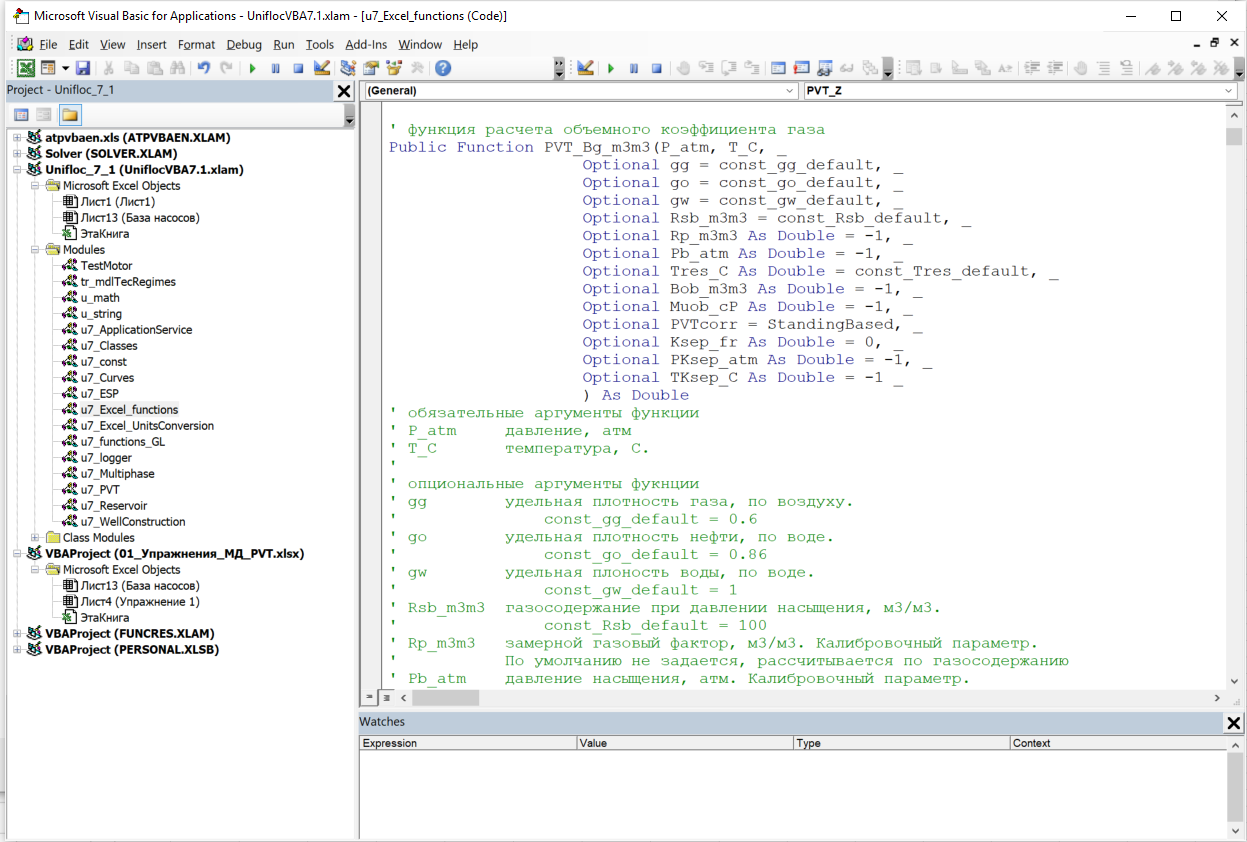
\includegraphics[width=1\linewidth]{vba_overview}
	\caption{Окно редактора VBE}
	\label{ris:VBA_overview}
\end{figure}


\subsection{Некоторые особенности VBA}
Строки, начинающиеся со знака ‘ являются комментариями. В VBE они выделяются зелёным цветом. На исполнение макросов не влияют.

Для многих макросов не обязательно задавать все параметры. Некоторые значения параметров могут не задаваться – тогда будут использованы значения параметров, принятые по умолчанию. Параметры, допускающие задание по умолчанию, помечены в исходном коде ключевым словом \mintinline{vb.net}{Optional}.

\section{Соглашения по названию функций и переменных \unf{}}
При создании макросов в основном использовались международные обозначения переменных, принятые в монографиях общества инженеров нефтяников SPE. Список наиболее употребляемых обозначений приведён в приложении. 

При создании макросов для обозначения переменных разработчики старались придерживаться следующих соглашений (впрочем,не всегда успешно):
\begin{itemize}
	\item название переменной или функции отражает физический смысл,
	\item лучше длинное и понятное название, чем короткое и непонятное, разделители слов в названиях - знаки подчёркивания (там, где это возможно),
	\item для расчётных функций название может содержать (последовательно) - префикс, указывающий группу функций, расчётное значение, ключевые параметры, на основе которых проводится расчёт, размерность результата,
	\item для минимизации путаницы с размерностями физических величин все размерные переменные в названии содержат явное указание размерности.
	\item названия единиц размерностей в переменных, данные в честь великих ученых пишутся с большой буквы (Pa, W, cP и тд, в отличии от atm, m, s) 
\end{itemize}

\section{Строковые переменные и параметры}
В надстройке унифлок, начиная с версии 7.26, активно используются строковые переменные для передачи параметров и настроек расчёта различных функций. Для кодирования значений в строках используется формат  \href{https://ru.wikipedia.org/wiki/JSON}{json}. 

Работа c json строками основана на макросах \href{https://github.com/VBA-tools/VBA-JSON}{github.com/VBA-tools/VBA-JSON} и \href{https://github.com/VBA-tools/VBA-Dictionary}{github.com/VBA-tools/VBA-Dictionary} by Tim Hall. Макросы и информация о их разработчиках в модуле JsonConverter и модуле класса Dictionary.

Для удобства работы со строковыми переменными реализован ряд пользовательских функций для работы с ними из рабочей книги Excel. Такие функции начинаются с префикса \mintinline{vb.net}{encode_} для функций формирующих строки json и с префикса \mintinline{vb.net}{decode_} для функций анализирующих строки json.

Строки в формате json используются для кодирования словарей и массивов значений.
\subsection{Строковая переменная - словарь}
В словаре хранятся поименованные переменные в виде пар - ключ, значение. В VBA функциональность словаря реализуется классом Dictionary, реализованным в виде отдельного модуля. Подробнее про реализацию словарей в \href{https://ru.wikipedia.org/wiki/JSON}{json} можно найти в википедии или других источниках в интернете.

Словари в \unf{} используется для работы с набора входных и выходных параметров, позволяя в одной ячейке записывать большой объем информации. Словари могут быть вложенные.

\subsection{Строковая переменная - массив}
В массиве или коллекции хранятся упорядоченные наборы переменных доступных по номеру. В VBA функциональность словаря реализуется классом Collection встроенным в объектную модель Excel. Подробнее про реализацию массивов или коллекций в \href{https://ru.wikipedia.org/wiki/JSON}{json} можно найти в википедии или других источниках в интернете.

Массивы в \unf{} как правило используются для хранения векторов численных значений (таблично заданных функций).

\section{Модель пласт - скважина - скважинное оборудование}

Набор функций \unf{} описывает математическую модель системы нефтедобычи, часто обозначаемой как модель "пласт - скважина - скважинное оборудование". Модель состоит из набора элементов - алгоритмов, описывающих ключевые физические процессы в системе нефтедобычи, существенно влияющие на результаты расчётов и на решения, которые могут быть приняты на основе расчётов.

К основным элементам системы можно отнести следующие модели:
\begin{itemize}
	\item модель физико-химических свойств пластовых флюидов;
	\item модель многофазного потока в трубопроводе, элементах инфраструктуры, скважинном оборудовании (например в штуцере);
	\item модель многофазного потока в стволе скважины;
	\item модель многофазного потока в пласте и призабойной зоне скважины;
	\item модель работы УЭЦН, в том числе многофазного потока в УЭЦН;
	\item модель работы скважины как системы "пласт - скважина - скважинное оборудование".
\end{itemize}

Ключевым параметром модели нефтедобычи является распределение давления и температуры в системе. Моделирование всех элементов системы направлено, как правило, на то, чтобы восстановить распределение давления.

Модель нефтедобычи напрямую отражается в объектной модели \unf{} и в наборе пользовательских функций. Пользовательскими функциями называются функции VBA которые могут быть напрямую использованы из рабочих книг Excel. 

Настоящее руководство пользователя описывает модель нефтедобычи и ее элементы как набор пользовательских функций, позволяющих провести расчёты из рабочей книги Excel. Более полный набор пользовательских функций и их описание можно найти в коде надстройки или в приложении "Автоматически сгенерированное описание".

Устройство и функциональность объектной модели \unf{} можно восстановить изучая исходный код расчётных модулей и комментарии в исходном коде. На текущий момент это наиболее надёжный, хотя и трудозатратный способ.           % Глава 1

\begin{center}
	{\large Расчет свойств потока флюидов при сепарации части свободного газа из потока}
\end{center}

Это описание содержит один из разделов руководства пользователя (мануала) к \unf{}. Полную версию мануала можно найти в репозитории \href{https://github.com/unifloc/unifloc_vba}{https://github.com/unifloc/unifloc\_vba}.



\chapter{PVT свойства флюидов}

\section{Преобразования потоков флюидов}

\subsection{PVT\_mod\_separate\_gas - сепарация части свободного газа из потока}
	Функция \mintinline{vb.net}{feed_mod_separate_gas} описывает процесс сепарации свободного газа из потока, например на приёме УЭЦН или в газосепараторе.
После отделения части свободного газа из потока, свойства потока по прежнему могут быть описаны в рамках модели нелетучей нефти, но с несколько модифицированными параметрами, учитывающими изменение фазового состава. Функция \mintinline{vb.net}{feed_mod_separate_gas} как раз рассчитывает такие параметры.

Алгоритм модификации параметров потока сводится к снижению газового фактора и расхода свободного газа, что удаляет газ из потока. При необходимости проводится корректировка давления насыщения $P_b$, объёмного коэффициента при давлении насыщения $B_{ob}$ и вязкости при давлении насыщения $\mu_{ob}$. 

Как правило, сепарация газа из потока проводится при относительно низком давлении, например при давлении на приёме насоса. Для потока в трубах предполагается, что  в каждый момент времени все фазы потока находятся в термодинамическом равновесии, что позволяет применять корреляции для нелетучей нефти.  Однако при поступлении частично дегазированного потока в насос, давление в нем резко повышается на значительную величину (для центробежного насоса с производительностью 150 м$^3$/сут, время прохождения потоком через одну ступень составляет около 0.02 сек \cite{diss_Igrevesky_ESP_gas}, таким образом через ЭЦН с 400 ступеней поток будет двигаться порядка 10 сек. При этом давление может повыситься на величину порядка 200 атм). За такое время свободный газ оставшийся в потоке может не успеть достичь термодинамического равновесия с нефтью, или другими слова может не успеть полностью раствориться. В работе Игревского В.И. \cite{diss_Igrevesky_ESP_gas} для учёта этого эффекта вводится коэффициент фазной неравновесности $K_f$

$$K_f = \frac{V_{sol}}{V_{eq}}= \frac{Q_{g.sol}}{Q_{g.eq}}$$

где  $V_{sol}$ - объем газа который растворится в нефти при движении через ЭЦН, $V_{sol}$ - объем газа который растворился бы в нефти при движении через ЭЦН при достижении термодинамического равновесия. 

Величина $K_f$ зависит среди прочих параметров от дисперсности потока (размера пузырьков газа), и объёмного газосодержания.  Для грубодисперсных смесей газ - вода можно принять $K_f=0.2$, для тонкодисперсных от $K_f=0.7$ до $K_f=1$. Для газонефтяных смесей можно считать $K_f=1$, то есть весь газ успевает раствориться в нефти при движении через ЭЦН. Это же предположении может быть использовано при движении газонефтяной смеси через трубы (скорость движения меньше в 5 - 10 раз в НКТ по сравнению с ЭЦН).

Для оценки влияния фазной неравновесности нефти на параметры многофазного потока при сепарации газа из потока можно использовать параметр \mintinline{vb.net}{gas_goes_into_solution}, который определяет значение   $K_f$

При условии $K_f = 0$ -- газ выделившийся в свободное состояние не растворяется обратно в нефти, при $K_f = 1$ -- весь газ может раствориться при повышении давления.

Новый газовый фактор и расход свободного газа, после сепарации газа можно найти из условия
\begin{equation}
	r_p^{new} = r_p - \left( r_p - r_s \right) k_{sep} 
\end{equation}

\begin{equation}
q_{gas}^{new} = q_{gas}(1-k_{sep}) 
\end{equation}

Максимально возможное значение газосодержания при повышении давления можно найти из выражения

\begin{equation} 
	r_s^{max} = r_s + \left( r_p - r_s \right) (1 - k_{sep}) *K_f 
	\label{eq:rsmax}
\end{equation}

При повышении давления часть газа может раствориться в нефти, что можно описать найдя величины $P_{b}^{new}$, $B_{ob}^{new}$,$\mu_{ob}^{new}$ c учетом максимально достижимого значения газосодержания (\ref{eq:rsmax}).

$$P_{b}^{new} = P_b(r_s^{max}) $$

$$B_{ob}^{new} = B_{ob}(r_s^{max}) $$

$$\mu_{ob}^{new} = \mu_{ob}(r_s^{max}) $$

где соответствующие зависимости $P_{b}(r_s)$, $B_{o}(r_s)$,$\mu_{o}(r_s)$ определяются в соответствии с заданным набором корреляций.

Рассмотрим пример 1 преобразования свойств потока флюида для следующего набора параметров:
параметры сепарации:  $k_{sep} = 0.5$ ,$p_{sep} = 50$   атма,	$t_{sep} = 90$   C ,$K_f = 0 $.    


\begin{table}[ht]
	\centering
	\caption{Исходные данные и результаты расчёта модификации флюида после частичной сепарации свободного газа. Пример 1, $K_f=0$ -- газ не растворяется при повышении давления.}
	\begin{tabular}{ |c|c|c|} 
		\hline
		Параметр & Исходные значения & Модифицированные \\ 
		\hline
		$\gamma_g$ 				&$0.9$	& $0.9$    \\ 
		$\gamma_o$ 					&$0.9$	& $0.9$   \\ 
		$r_{sb}$ ,  м$^3$/м$^3$ 		&$80$	& $25$ \\ 
		$P_b$ , атма 					&$130$	& $50$ 	 \\ 
		$T_{res} $,  C 					&$90$	& $90$ \\ 
		$B_{ob} $ , м$^3$/м$^3$  		&$1.2$	& $1.09$ \\ 
		$\mu_{ob}  $,  сП  				&$1$	& $1.96$   \\ 
		\hline
		$Q_{gas\ free}  $,  м$^3$/сут  	&$1000$	& $500$  \\ 
		$Q_{liq}  $,  м$^3$/сут  			&$15$	& $15$ \\ 
		$f_{w}  $,  \%  					&$1$	& $1$  \\ 
		$r_p  $,  м$^3$/м$^3$  			&$80$	& $52$ \\ 
		\hline
	\end{tabular}
	\label{table:separ_gas_table_1}
\end{table}

Зависимости свойств флюида от давления для примера 1 приведены на рисунке \ref{ris:separ_gas_plot_1}.

\begin{figure}[ht]
\begin{tikzpicture}[scale=0.65]
	\begin{axis}[
		xlabel=$P \;  atma$,
		ylabel=$r_s\; m^3/m^3$,
		legend pos=north west,
		title=газосодержание]
		\addplot table [y=rs, x=P]{data/separ_gas.txt};
		\addlegendentry{original}
		\addplot table [y=rs_mod, x=P]{data/separ_gas.txt};
		\addlegendentry{modified}
	\end{axis}
\end{tikzpicture}
\begin{tikzpicture}[scale=0.65]
	\begin{axis}[
		xlabel=$P \;  atma$,
		ylabel=$B_o\; m^3/m^3$,
		legend pos=north west,
		title=объемный коэффициент нефти]
		\addplot table [y=bo, x=P]{data/separ_gas.txt};
		\addlegendentry{original}
		\addplot table [y=bo_mod, x=P]{data/separ_gas.txt};
		\addlegendentry{modified}
	\end{axis}
\end{tikzpicture}
\begin{tikzpicture}[scale=0.65]
	\begin{axis}[
		xlabel=$P \;  atma$,
		ylabel=$\mu_o\; cP$,
		legend pos=north east,
		title=вязкость нефти]
		\addplot table [y=muo, x=P]{data/separ_gas.txt};
		\addlegendentry{original}
		\addplot table [y=muo_mod, x=P]{data/separ_gas.txt};
		\addlegendentry{modified}
	\end{axis}
\end{tikzpicture}
\caption{Зависимость параметров флюида от давления до и после сепарации части свободного газа. Пример 1, $K_f=0$ -- газ не растворяется при повышении давления}
\label{ris:separ_gas_plot_1}
\end{figure}

Из приведённых рисунков видно, что свойства нефти при давлении ниже давления сепарации не изменились, а новое давление насыщения показывает, что при повышении давления газ не будет растворяться в нефти. При этом значения параметров потока жидкости $Q_{liq}, f_w$ не изменяются.

При увеличении коэффициента неравновесности $K_f=0.9$ картина изменится - эффективное значение давления насыщения нефти вырастет, что позволит части газа раствориться. Ниже приводится пример 2, где также для наглядности изменён набор корреляций для следующего набора параметров: $k_{sep} = 0.5$ ,$p_{sep} = 50$   атма,	$t_{sep} = 90$   C ,$K_f = 0.9 $. Результаты расчета приведены в таблице \ref{table:separ_gas_table_2} и на   рисунке \ref{ris:separ_gas_plot_2}.

Следует отметить, что на величину эффективного значения давления насыщения может значительно влиять выбор набора корреляций для расчёта PVT свойств, в частности корреляции для зависимости давления насыщения от газосодержания при давлении насыщения. 

\begin{table}[H]
	\centering
	\caption{Исходные данные и результаты расчёта модификации флюида после частичной сепарации свободного газа. Пример 2, $K_f=0.9$ -- газ частично растворяется при повышении давления.}
	\begin{tabular}{ |c|c|c|} 
		\hline
		Параметр & Исходные значения & Модифицированные \\ 
		\hline
		$\gamma_g$ 				&$0.9$	& $0.9$    \\ 
		$\gamma_o$ 					&$0.9$	& $0.9$   \\ 
		$r_{sb}$ ,  м$^3$/м$^3$ 		&$80$	& $61$ \\ 
		$P_b$ , атма 					&$130$	& $84$ 	 \\ 
		$T_{res} $,  C 					&$90$	& $90$ \\ 
		$B_{ob} $ , м$^3$/м$^3$  		&$1.2$	& $1.16$ \\ 
		$\mu_{ob}  $,  сП  				&$1$	& $1.22$   \\ 
		\hline
		$Q_{gas\ free}  $,  м$^3$/сут  	&$1000$	& $500$  \\ 
		$Q_{liq}  $,  м$^3$/сут  			&$15$	& $15$ \\ 
		$f_{w}  $,  \%  					&$1$	& $1$  \\ 
		$r_p  $,  м$^3$/м$^3$  			&$80$	& $63$ \\ 
		\hline
	\end{tabular}
\label{table:separ_gas_table_2}
\end{table}

Зависимости свойств флюида от давления для примера 2 приведены на рисунке \ref{ris:separ_gas_plot_2}.

\begin{figure}[H]
\begin{tikzpicture}[scale=0.65]
	\begin{axis}[
		xlabel=$P \;  atma$,
		ylabel=$r_s\; m^3/m^3$,
		legend pos=north west,
		title=газосодержание]
		\addplot table [y=rs, x=P]{data/separ_gas_1.txt};
		\addlegendentry{original}
		\addplot table [y=rs_mod, x=P]{data/separ_gas_1.txt};
		\addlegendentry{modified}
	\end{axis}
\end{tikzpicture}
\begin{tikzpicture}[scale=0.65]
	\begin{axis}[
		xlabel=$P \;  atma$,
		ylabel=$B_o\; m^3/m^3$,
		legend pos=north west,
		title=объемный коэффициент нефти]
		\addplot table [y=bo, x=P]{data/separ_gas_1.txt};
		\addlegendentry{original}
		\addplot table [y=bo_mod, x=P]{data/separ_gas_1.txt};
		\addlegendentry{modified}
	\end{axis}
\end{tikzpicture}
\begin{tikzpicture}[scale=0.65]
	\begin{axis}[
		xlabel=$P \;  atma$,
		ylabel=$\mu_o\; cP$,
		legend pos=north east,
		title=вязкость нефти]
		\addplot table [y=muo, x=P]{data/separ_gas_1.txt};
		\addlegendentry{original}
		\addplot table [y=muo_mod, x=P]{data/separ_gas_1.txt};
		\addlegendentry{modified}
	\end{axis}
\end{tikzpicture}
\caption{Зависимость параметров флюида от давления до и после сепарации части свободного газа. Пример 2, $K_f=0.9$ -- газ частично растворяется при повышении давления}
\label{ris:separ_gas_plot_2}
\end{figure}


Часть настроек управляющая выводом результатов задается в виде закодированной строки в аргументе \mintinline{vb.net}{param}.

\begin{table}[H]
	\caption{Параметры функции \mintinline{vb.net}{feed_mod_separate_gas} передаваемые через аргумент -- \mintinline{vb.net}{param}}
	\label{table:param_list_feed_med_separation}
	\begin{tabular}{p{0.4\textwidth}p{0.55\textwidth}}
		\hline
		Ключ & Описание  \\ \hline
		\mintinline{vb.net}{show_array} & Показывать расширенные результаты расчета: 0 -- результат в виде одного числа (значение по умолчанию), 1 -- результат в виде массива.    \\ \hline
		
		\mintinline{vb.net}{show_log} & Показывать лог расчета в выводе. 0 -- лог выводиться не будет, 1 -- будет показан лог в виде json строки в массиве вывода. Большой размер лога может вызвать проблемы на некоторых версиях Excel.   \\ \hline
		
		\mintinline{vb.net}{gas_goes_into_solution} & Коэффициент фазной неравновесности $K_f$  \\ \hline
		
	\end{tabular}
\end{table}

При включенной опции \mintinline{vb.net}{show_array=1} результат выдается в виде двумерного массива значений - плоской таблицы. Результирующая таблица может быть непосредственно выведена в ячейки Excel (в версиях не поддерживающие динамические массивы необходимо использовать Cntrl-Shift-Enter для вывода результата в заранее выделенный диапазон ячеек) или получена в виде массива при вызове из VBA.

При выводе массива на лист Excel первая строка содержит значения параметров, вторая подписи к значениям. При выводе с использованием Cntrl-Shift-Enter можно вывести только первую строку параметров и распространить расчетную формулу протягиванием на несколько строк.

\begin{table}[H]
	\caption{Расширенный вывод функции \mintinline{vb.net}{feed_mod_separate_gas}}
	\label{table:param_list}
	\begin{tabular}{p{0.05\textwidth}p{0.3\textwidth}p{0.545\textwidth}}
		\hline
		№& Параметр & Описание  \\ \hline
		0 & \mintinline{vb.net}{feed} & json строка описывающая параметры модифицированного потока флюидов    \\ \hline
		
		1 & \mintinline{vb.net}{log} & Лог расчета, выводится при \mintinline{vb.net}{show_log = 1}  \\ \hline
		
	\end{tabular}
\end{table}
       % Глава PVT 
%	\section{Расчёт свойств потока}

В отличии от функций расчета PVT (физико-химических свойств флюидов) функции расчета свойства потока учитывают дополнительные параметры потока флюидов - $Q$ - дебит, объемный расход флюидов, $f_w$ - обводненность, $R_p$ - газовый фактор. В функциях свойств потока используется префикc \mintinline{vb.net}{feed_}.

Параметры потока, такие как расход ГЖС, доля газа в потоке, вязкость ГЖС важны для расчёта и анализа работы скважин и скважинного оборудования.


\subsection{feed\_q\_mix\_rc\_m3day – расход газожидкостной смеси}

Функция позволяет рассчитать объёмный расход газожидкостной смеси при заданных термобарических условиях. Объёмный расход ГЖС важен например для подбора УЭЦН в скважине, так как именно определяет в какой точке характеристики УЭЦН будет работать. При наличии свободного газа в потоке расход ГЖС может быть значительно больше расхода жидкости на поверхности фиксируемого расходомером.
$$Q_{mix,rc} = Q_{w,sc} B_w(P,T) + Q_{o,sc} B_o(P,T)  + Q_{o,sc}  (R_p - R_s(P,T)) B_g(P,T) $$

Расход ГЖС определяется как сумма расходов отдельных фаз, приведённых к соответствующим термобарическим условиям, с учётом того, что часть газа будет растворена в нефти.

\putlisting{listings/feed_q_mix_rc_m3day.lst}

\subsection{feed\_rho\_mix\_kgm3 – плотность газожидкостной смеси}

Функция позволяет рассчитать плотность газожидкостной смеси при заданных термобарических условиях. 
$$\rho_{mix,rc} = \left( \frac{\rho_{w,sc}}{B_w} f_w + \frac{\rho_{o,sc} +r_s \rho_{g,sc} }{B_o}(1-f_w) \right) (1-f_g) + \frac{ \rho_{g,sc} }{B_g} f_g $$

\putlisting{listings/feed_rho_mix_kgm3.lst}

\subsection{feed\_gas\_fraction\_d – доля газа в потоке}

Функция расчёта доли свободного газа в потоке (без учёта проскальзывания) в зависимости от термобарических условий для заданного флюида. 
$$f_g = \frac{Q_{gas\_rc} (1-k_{sep\_add})}{Q_{wat\_rc}+Q_{oil\_rc}+Q_{gas\_rc}(1-k_{sep\_add})} $$
где все объёмные расходы фаз приведены в соответствующих термобарических условиях, а $k_{sep,add}$ - дополнительный коэффициент сепарации, учитывающий удаление части свободного газа из потока.

Доля газа в потоке является одним из ключевых параметров ограничивающих производительность систем механизированной добычи - ЭЦН и других насосов.

\putlisting{listings/feed_gas_fraction_d.lst}

\subsection{feed\_p\_gas\_fraction\_atma – целевое давления для заданной доли газа в потоке}
Функция расчёта давления при котором достигается заданная доля свободного газа в потоке (без учёта проскальзывания). 
Значение давления при котором достигается определённая доля газа в потоке может быть найдено из решения уравнения, определяющего долю газа. 
$$f_g = \frac{Q_{gas\_rc} (1-k_{sep\_add})}{Q_{wat\_rc}+Q_{oil\_rc}+Q_{gas\_rc}(1-k_{sep\_add})} $$
Решение в \unf{} реализовано итеративное, методом деления отрезка пополам (дихотомия). При вызове функции пересчитывается состояние смеси с различными термобарическими условиями. Поэтому расчёт проводится относительно медленно. 

Задание $k_{sep\_add}$ позволит оценить целевое давление на приеме для ЭЦН при известной доли газа и известном ожидаемом значении сепарации газа. Отметим, что значение сепарации может быть оценено по корреляционным зависимостям. Но такие зависимости требуют знания давления сепарации, а следовательно их учет совместно с алгоритмом расчета давления при котором достигается определенная доля газа потребует итеративного решения, что выходит за рамки данной функции (например из за того, что это потребует задания дополнительных параметров конфигурации скважины).

\putlisting{listings/feed_p_gas_fraction_atma.lst}



\subsection{feed\_rp\_gas\_fraction\_m3m3 – целевой газовый фактор для заданной доли газа в потоке}
Функция расчёта газового фактора $R_p$ при котором достигается заданная доля свободного газа в потоке (без учёта проскальзывания) . 
Значение давления при котором достигается определённая доля газа в потоке может быть найдено из решения уравнения, определяющего долю газа. 
$$f_g = \frac{Q_{gas\_rc} (1-k_{sep\_add})}{Q_{wat\_rc}+Q_{oil\_rc}+Q_{gas\_rc}(1-k_{sep\_add})} $$

Решение в \unf{} реализовано с использованием итераций, методом деления отрезка пополам (дихотомия). При вызове функции  состояние смеси пересчитывается с различными термобарическими условиями. Поэтому расчёт проводится относительно медленно. 

Задание $k_{sep\_add}$ позволит оценить целевой газовый фактор при известной доли газа, давлении на приеме и ожидаемом значении сепарации газа. Отметим, что значение сепарации может быть оценено по корреляционным зависимостям. Но такие зависимости требуют знания как давления сепарации так и газового фактора, а следовательно их учет совместно с алгоритмом расчета газового фактора при котором достигается определенная доля газа потребует итеративного решения, что выходит за рамки данной функции (например из за того, что это потребует задания дополнительных параметров конфигурации скважины).

\putlisting{listings/feed_rp_gas_fraction_m3m3.lst}

\section{Сепарация газа в скважине}
В скважинах оборудованных системами механизированной добычи нефти важную роль играет процесс сепарации газа на приёме насоса. Под сепарацией газа понимается отделение части свободного газа из потока и перенаправление его по отдельному гидравлическому каналу на поверхность. В результате сепарации газа меняются свойства флюида, поступающего в насос и НКТ выше насоса. В частности меняются давление насыщения и газосодержание при давлении насыщения для флюида после сепарации. Более детальные модели флюида и сепарации могут показать, что при сепарации может поменяться и другие параметры - например состав газа после разгазирования. В модели нелетучей нефти реализованной в \unf{} эти эффекты не учитываются.


\begin{figure}[H]
	\centering
		

\tikzset{every picture/.style={line width=0.75pt}} %set default line width to 0.75pt        

\begin{tikzpicture}[x=0.75pt,y=0.75pt,yscale=-1,xscale=1]
%uncomment if require: \path (0,406); %set diagram left start at 0, and has height of 406

%Shape: Rectangle [id:dp04480742808021354] 
\draw  [fill={rgb, 255:red, 155; green, 155; blue, 155 }  ,fill opacity=1 ] (312,64.14) -- (351.5,64.14) -- (351.5,114.5) -- (312,114.5) -- cycle ;
%Shape: Rectangle [id:dp3210354209072095] 
\draw  [line width=2.25]  (259.42,64.14) -- (404.08,64.14) -- (404.08,352) -- (259.42,352) -- cycle ;
%Shape: Rectangle [id:dp11917689807401133] 
\draw  [fill={rgb, 255:red, 155; green, 155; blue, 155 }  ,fill opacity=1 ] (296.75,114.5) -- (366.75,114.5) -- (366.75,314.5) -- (296.75,314.5) -- cycle ;
%Shape: Rectangle [id:dp22447305445205257] 
\draw  [fill={rgb, 255:red, 255; green, 255; blue, 255 }  ,fill opacity=1 ] (305.89,238.94) -- (310.33,238.94) -- (310.33,269.56) -- (305.89,269.56) -- cycle ;
%Shape: Rectangle [id:dp05751039520762724] 
\draw  [fill={rgb, 255:red, 255; green, 255; blue, 255 }  ,fill opacity=1 ] (314.33,238.94) -- (318.78,238.94) -- (318.78,269.56) -- (314.33,269.56) -- cycle ;
%Shape: Rectangle [id:dp6083474962263296] 
\draw  [fill={rgb, 255:red, 255; green, 255; blue, 255 }  ,fill opacity=1 ] (322.11,238.94) -- (326.56,238.94) -- (326.56,269.56) -- (322.11,269.56) -- cycle ;
%Shape: Rectangle [id:dp9699991258462393] 
\draw  [fill={rgb, 255:red, 255; green, 255; blue, 255 }  ,fill opacity=1 ] (329.53,238.94) -- (333.97,238.94) -- (333.97,269.56) -- (329.53,269.56) -- cycle ;
%Shape: Rectangle [id:dp5276274421172025] 
\draw  [fill={rgb, 255:red, 255; green, 255; blue, 255 }  ,fill opacity=1 ] (337,238.94) -- (341.44,238.94) -- (341.44,269.56) -- (337,269.56) -- cycle ;
%Shape: Rectangle [id:dp8686039431642814] 
\draw  [fill={rgb, 255:red, 255; green, 255; blue, 255 }  ,fill opacity=1 ] (344.78,238.94) -- (349.22,238.94) -- (349.22,269.56) -- (344.78,269.56) -- cycle ;
%Shape: Rectangle [id:dp024923249699371652] 
\draw  [fill={rgb, 255:red, 255; green, 255; blue, 255 }  ,fill opacity=1 ] (352.56,238.94) -- (357,238.94) -- (357,269.56) -- (352.56,269.56) -- cycle ;
%Shape: Rectangle [id:dp24614630976896423] 
\draw  [fill={rgb, 255:red, 255; green, 255; blue, 255 }  ,fill opacity=1 ] (360.11,238.94) -- (364.56,238.94) -- (364.56,269.56) -- (360.11,269.56) -- cycle ;
%Shape: Rectangle [id:dp4580617305504924] 
\draw  [fill={rgb, 255:red, 255; green, 255; blue, 255 }  ,fill opacity=1 ] (298.78,238.94) -- (303.22,238.94) -- (303.22,269.56) -- (298.78,269.56) -- cycle ;
%Curve Lines [id:da46150758694693694] 
\draw [color={rgb, 255:red, 74; green, 144; blue, 226 }  ,draw opacity=1 ]   (282.2,352) .. controls (281.45,261.49) and (287.15,263.11) .. (299.52,257.34) ;
\draw [shift={(302.2,256)}, rotate = 511.33] [fill={rgb, 255:red, 74; green, 144; blue, 226 }  ,fill opacity=1 ][line width=0.08]  [draw opacity=0] (10.72,-5.15) -- (0,0) -- (10.72,5.15) -- (7.12,0) -- cycle    ;
%Shape: Circle [id:dp04721201185159396] 
\draw  [fill={rgb, 255:red, 255; green, 255; blue, 255 }  ,fill opacity=1 ] (304.99,174.01) .. controls (306.3,170.48) and (308.78,169.68) .. (310.52,172.22) .. controls (312.26,174.75) and (312.61,179.67) .. (311.3,183.19) .. controls (309.99,186.72) and (307.51,187.52) .. (305.77,184.98) .. controls (304.03,182.45) and (303.68,177.53) .. (304.99,174.01) -- cycle ;
%Shape: Circle [id:dp5883852152967295] 
\draw  [fill={rgb, 255:red, 255; green, 255; blue, 255 }  ,fill opacity=1 ] (350.59,174.01) .. controls (351.9,170.48) and (354.38,169.68) .. (356.12,172.22) .. controls (357.86,174.75) and (358.21,179.67) .. (356.9,183.19) .. controls (355.59,186.72) and (353.11,187.52) .. (351.37,184.98) .. controls (349.63,182.45) and (349.28,177.53) .. (350.59,174.01) -- cycle ;
%Curve Lines [id:da5619628529147929] 
\draw [color={rgb, 255:red, 74; green, 144; blue, 226 }  ,draw opacity=1 ]   (308.54,178.6) .. controls (288.8,173.65) and (285.1,176) .. (286.11,97.21) ;
\draw [shift={(286.14,94.8)}, rotate = 450.78] [fill={rgb, 255:red, 74; green, 144; blue, 226 }  ,fill opacity=1 ][line width=0.08]  [draw opacity=0] (10.72,-5.15) -- (0,0) -- (10.72,5.15) -- (7.12,0) -- cycle    ;
%Curve Lines [id:da7420889905281607] 
\draw [color={rgb, 255:red, 74; green, 144; blue, 226 }  ,draw opacity=1 ]   (269.4,352) .. controls (268.97,261.5) and (271.07,125.81) .. (271.01,97.45) ;
\draw [shift={(271,94.8)}, rotate = 449.4] [fill={rgb, 255:red, 74; green, 144; blue, 226 }  ,fill opacity=1 ][line width=0.08]  [draw opacity=0] (10.72,-5.15) -- (0,0) -- (10.72,5.15) -- (7.12,0) -- cycle    ;
%Curve Lines [id:da1955664158849284] 
\draw [color={rgb, 255:red, 74; green, 144; blue, 226 }  ,draw opacity=1 ]   (331.75,231.56) .. controls (331.45,207.23) and (331.44,241.87) .. (331.75,97) ;
\draw [shift={(331.75,94.8)}, rotate = 450.12] [fill={rgb, 255:red, 74; green, 144; blue, 226 }  ,fill opacity=1 ][line width=0.08]  [draw opacity=0] (10.72,-5.15) -- (0,0) -- (10.72,5.15) -- (7.12,0) -- cycle    ;
%Curve Lines [id:da5073323315189147] 
\draw [color={rgb, 255:red, 74; green, 144; blue, 226 }  ,draw opacity=1 ]   (331.75,230.44) .. controls (330.74,183.59) and (324.76,182.05) .. (316.18,179.48) ;
\draw [shift={(313.4,178.58)}, rotate = 379.94] [fill={rgb, 255:red, 74; green, 144; blue, 226 }  ,fill opacity=1 ][line width=0.08]  [draw opacity=0] (10.72,-5.15) -- (0,0) -- (10.72,5.15) -- (7.12,0) -- cycle    ;
%Curve Lines [id:da18312163514470803] 
\draw [color={rgb, 255:red, 74; green, 144; blue, 226 }  ,draw opacity=1 ]   (331.75,231.17) .. controls (330.77,185.6) and (339.02,182.33) .. (345.86,179.93) ;
\draw [shift={(348.56,178.89)}, rotate = 514.89] [fill={rgb, 255:red, 74; green, 144; blue, 226 }  ,fill opacity=1 ][line width=0.08]  [draw opacity=0] (10.72,-5.15) -- (0,0) -- (10.72,5.15) -- (7.12,0) -- cycle    ;
%Curve Lines [id:da5609474333970248] 
\draw [color={rgb, 255:red, 74; green, 144; blue, 226 }  ,draw opacity=1 ]   (353.74,178.6) .. controls (374.5,175.74) and (380.34,176.04) .. (381.54,97.21) ;
\draw [shift={(381.57,94.8)}, rotate = 450.78] [fill={rgb, 255:red, 74; green, 144; blue, 226 }  ,fill opacity=1 ][line width=0.08]  [draw opacity=0] (10.72,-5.15) -- (0,0) -- (10.72,5.15) -- (7.12,0) -- cycle    ;
%Curve Lines [id:da942989625089206] 
\draw [color={rgb, 255:red, 74; green, 144; blue, 226 }  ,draw opacity=1 ]   (394.29,352) .. controls (393.86,261.5) and (394.33,125.81) .. (394.16,97.45) ;
\draw [shift={(394.14,94.8)}, rotate = 449.4] [fill={rgb, 255:red, 74; green, 144; blue, 226 }  ,fill opacity=1 ][line width=0.08]  [draw opacity=0] (10.72,-5.15) -- (0,0) -- (10.72,5.15) -- (7.12,0) -- cycle    ;
%Curve Lines [id:da2534809401724647] 
\draw [color={rgb, 255:red, 74; green, 144; blue, 226 }  ,draw opacity=1 ]   (381.98,352) .. controls (381.21,259.56) and (377.98,263.5) .. (358.91,258.24) ;
\draw [shift={(356.11,257.42)}, rotate = 377.19] [fill={rgb, 255:red, 74; green, 144; blue, 226 }  ,fill opacity=1 ][line width=0.08]  [draw opacity=0] (10.72,-5.15) -- (0,0) -- (10.72,5.15) -- (7.12,0) -- cycle    ;
%Shape: Rectangle [id:dp25186132731738486] 
\draw  [color={rgb, 255:red, 255; green, 255; blue, 255 }  ,draw opacity=1 ][fill={rgb, 255:red, 255; green, 255; blue, 255 }  ,fill opacity=1 ] (249.86,58.29) -- (411.29,58.29) -- (411.29,70.29) -- (249.86,70.29) -- cycle ;
%Shape: Rectangle [id:dp3766484711992675] 
\draw  [color={rgb, 255:red, 255; green, 255; blue, 255 }  ,draw opacity=1 ][fill={rgb, 255:red, 255; green, 255; blue, 255 }  ,fill opacity=1 ] (251.43,346.29) -- (414.71,346.29) -- (414.71,358.57) -- (251.43,358.57) -- cycle ;





\end{tikzpicture}
		\caption{Схема линий тока газа на приеме ЭЦН}
		\label{ris:separation_scheme}
\end{figure}

В скважине с ЭЦН работают два механизма сепарации свободного газа из потока, схематично показанные на рисунке \ref{ris:separation_scheme} - естественная или натуральная сепарация газа, когда часть свободного газа за счет сил всплытия проходит мимо приема насоса и искусственная сепарация с применением газосепаратора, когда часть свободного газа выталкивается из насоса, обычно за счет центробежных сил. 

Оценка этих механизмов, а также расчёт общей сепарации могут быть проведены приведёнными ниже функциями.

\subsection{well\_ksep\_natural\_d – естественная сепарация газа}
Функция рассчитывает естественную сепарацию газа на приёме насоса в скважине с использованием корреляции Маркеса \cite{Marquez_2003} . Результат - безразмерная величина в диапазоне от 0 до 1. 

\putlisting{listings/well_ksep_natural_d.lst}

%\subsection{ESP\_ksep\_gasseparator\_d – сепарация газа роторным газосепаратором}
%Функция рассчитывает сепарацию газа с использованием роторного газосепаратора, являющегося обычно частью компоновки УЭЦН. Данный расчет основан на результатах испытания характеристик роторных газосепараторов, выполненных в РГУ нефти и газа имени И.М.Губкина \cite{SPE_117415_2008}. 

%Следует отметить, что несмотря на хорошее соответствие промысловых исследований и расчетов с использованием корреляции для естественной и искусственной сепарации \cite{SPE_117415_2008} к результатам стендовых исследований стоит относится с осторожностью. Основой осторожности могут быть следующие соображения: характеристики различных газосепараторов достаточно сильно отличаются друг от друга - есть удачные конструкции и не очень, при этом результаты стендовых испытаний доступны только для ограниченного набора конструкций, стендовые условия достаточно сильно отличаются от скважинных - ниже давление, другие модельные рабочие жидкости, точно оценить коэффициент сепарации газосепаратора в промысловых условиях затруднительно - набор таких данных для сравнения ограничен. 

%Тем не менее изучение результатов стендовых испытаний полезно при проведении расчетов и развивает инженерную интуицию. 

%\putlisting{listings/ESP_gassep_ksep_d.lst}


\subsection{well\_ksep\_total\_d – общая сепарация газа}

Функция рассчитывает полную сепарацию газа на приёме насосе в скважине по известным значениям естественной сепарации газа и коэффициента сепарации газосепаратора. Результат - безразмерная величина в диапазоне от 0 до 1. 

$$K_{sep\_total} = K_{sep\_nat} + (1-K_{sep\_nat}) K_{sep\_gassep}$$

\putlisting{listings/well_ksep_total_d.lst}

\section{Расчёт многофазного потока в штуцере}


Штуцер или локальное гидравлическое сопротивление - элемент скважины или системы трубопроводов, применяемых для создания дополнительного перепада давления в системе и ограничения потока. 
Возможны различные варианты реализации штуцера - со штуцерной камерой, с угловым краном, позволяющим менять диаметр штуцера и другие.
Ключевым параметром штуцера является диаметр \(d_{choke} \) определяющий его способность к ограничению потока. 

\begin{figure}[H]
	\begin{center}
	    		% https://www.mathcha.io/editor# использован для построения картинок



		
		\tikzset{every picture/.style={line width=0.75pt}} %set default line width to 0.75pt        
		
		\begin{tikzpicture}[x=0.75pt,y=0.75pt,yscale=-1,xscale=1]
		%uncomment if require: \path (0,300); %set diagram left start at 0, and has height of 300
		
		%Shape: Rectangle [id:dp8089540927658381] 
		\draw  [color={rgb, 255:red, 0; green, 0; blue, 0 }  ,draw opacity=1 ][fill={rgb, 255:red, 155; green, 155; blue, 155 }  ,fill opacity=1 ][line width=2.25]  (92,42) -- (570.83,42) -- (570.83,56.33) -- (92,56.33) -- cycle ;
		%Shape: Rectangle [id:dp7288541809010827] 
		\draw  [fill={rgb, 255:red, 155; green, 155; blue, 155 }  ,fill opacity=1 ][line width=2.25]  (92,227) -- (570.83,227) -- (570.83,241) -- (92,241) -- cycle ;
		%Shape: Rectangle [id:dp666453613189492] 
		\draw  [color={rgb, 255:red, 0; green, 0; blue, 0 }  ,draw opacity=1 ][fill={rgb, 255:red, 155; green, 155; blue, 155 }  ,fill opacity=1 ][line width=2.25]  (323.83,56.33) -- (341.17,56.33) -- (341.17,118.67) -- (323.83,118.67) -- cycle ;
		%Shape: Rectangle [id:dp015115451250117262] 
		\draw  [fill={rgb, 255:red, 155; green, 155; blue, 155 }  ,fill opacity=1 ][line width=2.25]  (323.83,165) -- (341.83,165) -- (341.83,226.83) -- (323.83,226.83) -- cycle ;
		%Right Arrow [id:dp058738740185342975] 
		\draw   (231,133.5) -- (274.56,133.5) -- (274.56,127) -- (289.83,140) -- (274.56,153) -- (274.56,146.5) -- (231,146.5) -- cycle ;
		%Straight Lines [id:da28021737295590965] 
		\draw    (341,119) -- (455,119) ;
		
		
		%Straight Lines [id:da8575303554097866] 
		\draw    (341,165) -- (455,165) ;
		
		
		%Straight Lines [id:da44299065539354565] 
		\draw    (440,120.89) -- (440,161.67) ;
		\draw [shift={(440,163.67)}, rotate = 270.28] [color={rgb, 255:red, 0; green, 0; blue, 0 }  ][line width=0.75]    (10.93,-3.29) .. controls (6.95,-1.4) and (3.31,-0.3) .. (0,0) .. controls (3.31,0.3) and (6.95,1.4) .. (10.93,3.29)   ;
		\draw [shift={(440.22,118.89)}, rotate = 90.28] [color={rgb, 255:red, 0; green, 0; blue, 0 }  ][line width=0.75]    (10.93,-3.29) .. controls (6.95,-1.4) and (3.31,-0.3) .. (0,0) .. controls (3.31,0.3) and (6.95,1.4) .. (10.93,3.29)   ;
		%Shape: Rectangle [id:dp8558237837917941] 
		\draw  [color={rgb, 255:red, 155; green, 155; blue, 155 }  ,draw opacity=1 ][fill={rgb, 255:red, 155; green, 155; blue, 155 }  ,fill opacity=1 ] (325.94,51) -- (339.28,51) -- (339.28,91) -- (325.94,91) -- cycle ;
		%Shape: Rectangle [id:dp8173981538013828] 
		\draw  [color={rgb, 255:red, 155; green, 155; blue, 155 }  ,draw opacity=1 ][fill={rgb, 255:red, 155; green, 155; blue, 155 }  ,fill opacity=1 ] (325.94,196) -- (339.94,196) -- (339.94,236) -- (325.94,236) -- cycle ;
		
		% Text Node
		\draw (207.67,141.04) node [scale=1.2,rotate=-0.61]  {$Q_{liq}$};
		% Text Node
		\draw (472,142.04) node [scale=1.2,rotate=-0.61]  {$d_{choke}$};
		% Text Node
		\draw (117.33,142) node [scale=1.44,rotate=-0.74]  {$P_{in}$};
		% Text Node
		\draw (540.67,140.37) node [scale=1.44,rotate=-0.74]  {$P_{out}$};
		
		
		\end{tikzpicture}
		\caption{Схема локального гидравлического сопротивления - штуцера}
		\label{ris:Pipe_choke}
	\end{center}
\end{figure}

Как и у любого элемента гидравлического потока есть три ключевых параметра - давление на входе \( P_{in} \), давление на выходе \(P_{out}\)  и расход газожидкостной смеси, обычно задаваемый в стандартных условиях \(Q_{liq} \). Задание любых двух элементов позволяет вычислить третий. При задании трех элементов модель штуцера может быть настроена на замеры за счёт подбора калибровочного параметра.

Следует обратить внимание, расчёт перепада давления в штуцере сильно зависит от направления расчёта. При фиксированном давлении на выходе $P_{out}$, что для скважины и штуцера на устье соответствует заданному давлению в линии, для любого расхода ГЖС через штуцер можно найти соответствующее значение давления на входе, пример показан на рисунке \ref{ris:choke_out_curves}.
 
\begin{figure}[H]
	
	\begin{center}
		
		\newcommand{\dPipeDataFile}{data/choke1.prn}
		\begin{tikzpicture}[scale=1]
		\begin{axis}[
		width=14cm,
		height=8cm,
		xlabel=$Q\; m^3 / day$,
		ylabel=$P_{in} \; atma$,
		legend pos=south east,
		title=Перепад давления в штуцере]
		\addplot table [y=Pout_1, x=Q]{\dPipeDataFile};
		\addlegendentry{$P_{out}=1$}
		\addplot table [y=Pout_5, x=Q]{\dPipeDataFile};
		\addlegendentry{$P_{out}=5$}
		\addplot table [y=Pout_10, x=Q]{\dPipeDataFile};
		\addlegendentry{$P_{out}=10$}
		\addplot table [y=Pout_15, x=Q]{\dPipeDataFile};
		\addlegendentry{$P_{out}=15$}
		\addplot table [y=Pout_20, x=Q]{\dPipeDataFile};
		\addlegendentry{$P_{out}=20$}
		\addplot table [y=Pout_30, x=Q]{\dPipeDataFile};
		\addlegendentry{$P_{out}=30$}
		\end{axis}
		\end{tikzpicture}
		
		
		\caption{Кривые зависимости давления на входе в штуцер от дебита при фиксированном давлении на выходе из штуцера $P_{out}$}
		\label{ris:choke_out_curves}
		
	\end{center}
\end{figure} 

А вот при фиксированном давлении на входе $P_{in}$ или фиксированном буферном давлении $P_{buf}$ не для всякого расхода ГЖС можно рассчитать давление на выходе, смотри рисунок \ref{ris:choke_in_curves}. При фиксированном давлении на входе $P_{in}$ существует максимальный расход ГЖС, который можно прокачать через штуцер с заданным диаметром проходного канала. Такой расход называется критическим. При критическом расходе в канале штуцера скорость потока достигает скорости звука и давление на входе перестаёт зависеть от давления за штуцером. Величина критического расхода через штуцер зависит от давления на входе, поскольку с повышением давления увеличивается скорость звука в среде.

Вертикальная линия на графике зависимости давления на выходе $P_{out}$ от дебита при критическом расходе показывает, что давление не определяется однозначно, а может принимать любое значение на вертикальной линии. Подобная неоднозначность расчётного давления на выходе штуцера может осложнять расчёты и должна учитываться инженером разрабатывающим расчётный модуль или проводящим расчёты.

\begin{figure}[H]
	
	\begin{center}
		
		\newcommand{\dPipeDataFile}{data/choke2.prn}
		\begin{tikzpicture}[scale=1]
		\begin{axis}[
		width=14cm,
		height=8cm,
		xlabel=$Q\; m^3 / day$,
		ylabel=$P_{out} \; atma$,
		legend pos=south east,
		title=Перепад давления в штуцере]
		\addplot table [y=Pin_10, x=Q]{\dPipeDataFile};
		\addlegendentry{$P_{in}=10$}
		\addplot table [y=Pin_15, x=Q]{\dPipeDataFile};
		\addlegendentry{$P_{in}=15$}
		\addplot table [y=Pin_20, x=Q]{\dPipeDataFile};
		\addlegendentry{$P_{in}=20$}
		\addplot table [y=Pin_25, x=Q]{\dPipeDataFile};
		\addlegendentry{$P_{in}=25$}
		\addplot table [y=Pin_30, x=Q]{\dPipeDataFile};
		\addlegendentry{$P_{in}=30$}
		\addplot table [y=Pin_35, x=Q]{\dPipeDataFile};
		\addlegendentry{$P_{in}=35$}
		\end{axis}
		\end{tikzpicture}
		
		
		\caption{Кривые зависимости давления на выходе из штуцера от дебита при фиксированном давлении на входе в штуцер $P_{in}$}
		\label{ris:choke_in_curves}
		
	\end{center}
\end{figure} 

Функции расчета штуцера позволяют настроить модель штуцера на замерные данные. Настройка проводится за счет безразмерного параметра калибровки $c_{calibr}$, в коде \mintinline{vb.net}{calibr}. 
Параметр калибровки $c_{calibr}$ применяется как множитель на дебит при расчете характеристики штуцера. 
$$Q_{real} = Q_{calc} * c_{calibr}$$
Таким образом $c_{calibr}=1$ отключает калибровку. А изменение $c_{calibr}$ позволит изменить характеристику штуцера для согласования с измерениями, пример показан на рисунке \ref{ris:choke_cal_curves}.

\begin{figure}[H]
	
	\begin{center}
		
		\newcommand{\dPipeDataFile}{data/choke3.prn}
		\begin{tikzpicture}[scale=1]
		\begin{axis}[
		width=14cm,
		height=6cm,
		xlabel=$Q\; m^3 / day$,
		ylabel=$P_{out} \; atma$,
		legend pos=south west,
		title=Пример калибровки модели штуцера]
		\addplot table [y=cal_1, x=Q]{\dPipeDataFile};
		\addlegendentry{$c_{calibr}=1$}
		\addplot table [y=cal_1.2, x=Q]{\dPipeDataFile};
		\addlegendentry{$c_{calibr}=1.2$}
		\end{axis}
		\end{tikzpicture}
		
		
		\caption{Кривые зависимости давления на выходе из штуцера от дебита при фиксированном давлении на входе в штуцер $P_{in}$}
		\label{ris:choke_cal_curves}
		
	\end{center}
\end{figure}  

Все функции для расчета штуцера содержат в названии слово \mintinline{vb.net}{choke}. 
 
Результатом работы функций является массив либо число либо массив значений содержащий давление на входе в штуцер $P_{in}$, давление на выходе из штуцера $P_{out}$, температуру потока в штуцере $T_{choke}$, калибровочный коэффициент штуцера $c_{calibr}$ и другие параметры. Регулируется опцией \mintinline{vb.net}{show_array=1} в аргументе \mintinline{vb.net}{param}.  Выходной массив содержит две строки - в первой находятся значения, во второй подписи. Это позволяет при необходимости вывести только значения в той же строке в которой проводился расчет. 

Для вывода массива в Excel следует выбрать необходимый диапазон ячеек, в который будут выводится результаты в виде массива, затем ввести в адресную строку вызов функции и нажать комбинацию клавиш - Cntrl-Shift-Enter. После этого название функции в адресной строке должно отображаться в фигурных скобках, рисунок \ref{ris:choke_array_out}. При необходимости внести коррективы в вызов функции также необходимо подтверждать свои действия комбинацией клавиш Cntrl-Shift-Enter.


\begin{figure}[ht]
	\center{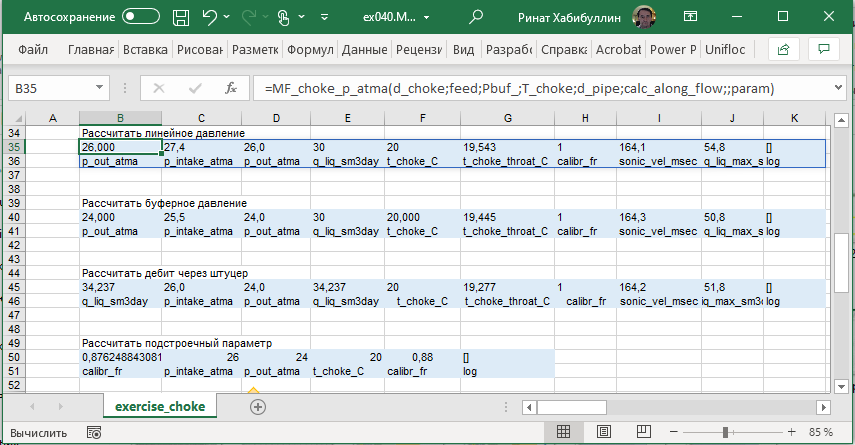
\includegraphics[width=1\linewidth]{choke_array_out}}
	\caption{Пример вывода результата расчета в массив}
	\label{ris:choke_array_out}
\end{figure}

%Функции расчёта штуцера поддерживают вычисления потока чистого газа через штуцер. Для этого в PVT строке надо установить \mintinline{vb.net}{gas_only=True} и задать расход газа параметром \mintinline{vb.net}{q_gas_sm3day} в соответствующей функции. 

\subsection{MF\_choke\_p\_atma – Расчет давления на входе или на выходе штуцера}
Функция позволяет рассчитать давление на входе или выходе штуцера по известному давлению на противоположном конце при известных параметрах потока (дебите жидкости, обводнённости, газовому фактору). Расчёт проводится по корреляции Перкинса \cite{Perkins_1993} с учётом многофазного потока. 
 
\putlisting{listings/MF_choke_p_atma.lst}

Часть настроек управляющая выводом результатов задается в виде закодированной строки в аргументе \mintinline{vb.net}{param}.

\begin{table}[H]
	\caption{Параметры функции \mintinline{vb.net}{MF_choke_p_atma} передаваемые через аргумент -- \mintinline{vb.net}{param}}
	\label{table:param_list}
	\begin{tabular}{p{0.2\textwidth}p{0.75\textwidth}}
		\hline
		Ключ & Описание  \\ \hline
		\mintinline{vb.net}{show_array} & Показывать расширенные результаты расчета: 0 -- результат в виде одного числа (значение по умолчанию), 1 -- результат в виде массива.    \\ \hline
		
		\mintinline{vb.net}{show_log} & Показывать лог расчета в выводе. 0 -- лог выводиться не будет, 1 -- будет показан лог в виде json строки в массиве вывода. Большой размер лога может вызвать проблемы на некоторых версиях Excel.   \\ \hline
		
		\mintinline{vb.net}{num_value} & Номер параметра выводимого на первом месте. Позволяет подменить выводимый параметр при \mintinline{vb.net}{show_array=0} на необходимый. Номера можно определить по расширенному выводу при \mintinline{vb.net}{show_array=1}  \\ \hline
		
	\end{tabular}
\end{table}

При включенной опции \mintinline{vb.net}{show_array=1} результат выдается в виде двумерного массива значений - плоской таблицы. Результирующая таблица может быть непосредственно выведена в ячейки Excel (в версиях не поддерживающие динамические массивы необходимо использовать Cntrl-Shift-Enter для вывода результата в заранее выделенный диапазон ячеек) или получена в виде массива при вызове из VBA.

При выводе массива на лист Excel первая строка содержит значения параметров, вторая подписи к значениям. При выводе с использованием Cntrl-Shift-Enter можно вывести только первую строку параметров и распространить расчетную формулу "протягиванием" на несколько строк.

\begin{table}[H]
	\caption{Расширенные результаты расчета}
	\label{table:param_list}
	\begin{tabular}{p{0.05\textwidth}p{0.3\textwidth}p{0.5\textwidth}}
		\hline
		№& Параметр & Описание  \\ \hline
		0 & Параметр по умолчанию & Параметр который выводится при \mintinline{vb.net}{show_array=0} или при подавлении вывода массива. Может быть настроен опцией  \mintinline{vb.net}{num_value}    \\ \hline
		
		1 & \mintinline{vb.net}{p_intake_atma} & Давление на входе в штуцер, атм    \\ \hline
		2 & \mintinline{vb.net}{p_out_atma} & Давление на выходе из штуцер, атм    \\ \hline
		3 & \mintinline{vb.net}{q_liq_sm3day} & Расход жидкости в стандартных условиях через штуцер, м$^3$/сут    \\ \hline
		4 & \mintinline{vb.net}{t_choke_C} & Температура флюида на входе и выходе из штуцера, С  \\ \hline
		5 & \mintinline{vb.net}{t_choke_throat_C} & Температура флюида внутри штуцера, в области с наибольшей скоростью, С  \\ \hline
		6 & \mintinline{vb.net}{calibr_fr} & Калибровочный параметр для модели штуцера  \\ \hline
		7 & \mintinline{vb.net}{sonic_vel_msec} & Скорость звука для флюида в проходном сечении штуцера, м/сек  \\ \hline
		8 & \mintinline{vb.net}{q_liq_max_sm3day} & Максимально возможный дебит жидкости через штуцер при заданном давлении на входе, м$^3$/сут  \\ \hline
		9 & \mintinline{vb.net}{log} & Лог расчета, выводится при \mintinline{vb.net}{show_log = 1}  \\ \hline
		
	\end{tabular}
\end{table}

При расчете предполагается, что температура флюида в штуцере не изменяется, однако в проходном сечении штуцера в корреляции Перкинса учитывается снижение температуры газа при снижении давления. Расчетное значение температуры выводится в как  \mintinline{vb.net}{t_choke_throat_C}. Также выводится скорость звука в сечении \mintinline{vb.net}{sonic_vel_msec}, которая достигается при критическом потока флюида и также выводится дебит \mintinline{vb.net}{q_liq_max_sm3day} при котором критический поток достигается. 



\subsection{MF\_choke\_q\_sm3day – функция расчёта дебита жидкости через штуцер}
Функция позволяет рассчитать по известному буферному давлению и линейному давлению дебит жидкости. Расчет  проводится по корреляции Перкинса \cite{Perkins_1993} с учетом многофазного потока.  

\putlisting{listings/MF_choke_q_sm3day.lst}

Часть настроек управляющая выводом результатов задается в виде закодированной строки в аргументе \mintinline{vb.net}{param}.

\begin{table}[H]
	\caption{Параметры функции  \mintinline{vb.net}{MF_choke_q_sm3day} передаваемые через аргумент -- \mintinline{vb.net}{param}}
	\label{table:param_list}
	\begin{tabular}{p{0.2\textwidth}p{0.75\textwidth}}
		\hline
		Ключ & Описание  \\ \hline
		\mintinline{vb.net}{show_array} & Показывать расширенные результаты расчета: 0 -- результат в виде одного числа (значение по умолчанию), 1 -- результат в виде массива.    \\ \hline
		
		\mintinline{vb.net}{show_log} & Показывать лог расчета в выводе. 0 -- лог выводиться не будет, 1 -- будет показан лог в виде json строки в массиве вывода. Большой размер лога может вызвать проблемы на некоторых версиях Excel.   \\ \hline
		
		\mintinline{vb.net}{num_value} & Номер параметра выводимого на первом месте. Позволяет подменить выводимый параметр при \mintinline{vb.net}{show_array=0} на необходимый. Номера можно определить по расширенному выводу при \mintinline{vb.net}{show_array=1}  \\ \hline
		
	\end{tabular}
\end{table}

При включенной опции \mintinline{vb.net}{show_array=1} результат выдается в виде двумерного массива значений - плоской таблицы. Результирующая таблица может быть непосредственно выведена в ячейки Excel (в версиях не поддерживающие динамические массивы необходимо использовать Cntrl-Shift-Enter для вывода результата в заранее выделенный диапазон ячеек) или получена в виде массива при вызове из VBA.

При выводе массива на лист Excel первая строка содержит значения параметров, вторая подписи к значениям. При выводе с использованием Cntrl-Shift-Enter можно вывести только первую строку параметров и распространить расчетную формулу "протягиванием" на несколько строк.

\begin{table}[H]
	\caption{Расширенный вывод функции \mintinline{vb.net}{MF_choke_q_sm3day}}
	\label{table:param_list_choke_q}
	\begin{tabular}{p{0.05\textwidth}p{0.3\textwidth}p{0.5\textwidth}}
		\hline
		№& Параметр & Описание  \\ \hline
		0 & Параметр по умолчанию & Параметр который выводится при \mintinline{vb.net}{show_array=0} или при подавлении вывода массива. Может быть настроен опцией  \mintinline{vb.net}{num_value}    \\ \hline
		
		1 & \mintinline{vb.net}{p_intake_atma} & Давление на входе в штуцер, атм    \\ \hline
		2 & \mintinline{vb.net}{p_out_atma} & Давление на выходе из штуцер, атм    \\ \hline
		3 & \mintinline{vb.net}{q_liq_sm3day} & Расход жидкости в стандартных условиях через штуцер, м$^3$/сут    \\ \hline
		4 & \mintinline{vb.net}{t_choke_C} & Температура флюида на входе и выходе из штуцера, С  \\ \hline
		5 & \mintinline{vb.net}{t_choke_throat_C} & Температура флюида внутри штуцера, в области с наибольшей скоростью, С  \\ \hline
		6 & \mintinline{vb.net}{calibr_fr} & Калибровочный параметр для модели штуцера  \\ \hline
		7 & \mintinline{vb.net}{sonic_vel_msec} & Скорость звука для флюида в проходном сечении штуцера, м/сек  \\ \hline
		8 & \mintinline{vb.net}{q_liq_max_sm3day} & Максимально возможный дебит жидкости через штуцер при заданном давлении на входе, м$^3$/сут  \\ \hline
		9 & \mintinline{vb.net}{log} & Лог расчета, выводится при \mintinline{vb.net}{show_log = 1}  \\ \hline
		
	\end{tabular}
\end{table}

%Если при формировании PVT строки задать параметр \mintinline{vb.net}{gas_only=True}, то расчет будет проведен для потока газа.

\subsection{MF\_choke\_calibr\_fast – простая и быстрая функция настройки модели штуцера}
Функция позволяет рассчитать корректирующий фактор для модели штуцера, позволяющий согласовать результаты замеров давления и дебита. Расчет проводится по корреляции Перкинса \cite{Perkins_1993} с учетом многофазного потока.  

Это быстрый способ расчета калибровочного коэффициента. По факту он просто вычисляется исходя из модели штуцера.
В более сложной функции калибровки \mintinline{vb.net}{MF_calibr_choke} расчет будет проводится дольше, так как подстроечные параметры подбираются итеративным алгоритмом, зато имеется возможность подбора нескольких различных параметров.

\putlisting{listings/MF_choke_calibr_fast.lst}

%Если при формировании PVT строки задать параметр \mintinline{vb.net}{gas_only=True}, то расчет проведен не будет.
Часть настроек управляющая выводом результатов задается в виде закодированной строки в аргументе \mintinline{vb.net}{param}.

\begin{table}[H]
	\caption{Параметры функции  \mintinline{vb.net}{MF_choke_calibr_fast} передаваемые через аргумент -- \mintinline{vb.net}{param}}
	\label{table:param_list}
	\begin{tabular}{p{0.2\textwidth}p{0.75\textwidth}}
		\hline
		Ключ & Описание  \\ \hline
		\mintinline{vb.net}{show_array} & Показывать расширенные результаты расчета: 0 -- результат в виде одного числа (значение по умолчанию), 1 -- результат в виде массива.    \\ \hline
		
		\mintinline{vb.net}{show_log} & Показывать лог расчета в выводе. 0 -- лог выводиться не будет, 1 -- будет показан лог в виде json строки в массиве вывода. Большой размер лога может вызвать проблемы на некоторых версиях Excel.   \\ \hline
		
		\mintinline{vb.net}{num_value} & Номер параметра выводимого на первом месте. Позволяет подменить выводимый параметр при \mintinline{vb.net}{show_array=0} на необходимый. Номера можно определить по расширенному выводу при \mintinline{vb.net}{show_array=1}  \\ \hline
	\end{tabular}
\end{table}

При включенной опции \mintinline{vb.net}{show_array=1} результат выдается в виде двумерного массива значений - плоской таблицы. Результирующая таблица может быть непосредственно выведена в ячейки Excel (в версиях не поддерживающие динамические массивы необходимо использовать Cntrl-Shift-Enter для вывода результата в заранее выделенный диапазон ячеек) или получена в виде массива при вызове из VBA.

При выводе массива на лист Excel первая строка содержит значения параметров, вторая подписи к значениям. При выводе с использованием Cntrl-Shift-Enter можно вывести только первую строку параметров и распространить расчетную формулу "протягиванием" на несколько строк.

\begin{table}[H]
	\caption{Расширенный вывод функции \mintinline{vb.net}{MF_choke_calibr_fast}}
	\label{table:param_list_choke_q}
	\begin{tabular}{p{0.05\textwidth}p{0.3\textwidth}p{0.5\textwidth}}
		\hline
		№& Параметр & Описание  \\ \hline
		0 & \mintinline{vb.net}{calibr_fr} & Параметр калибровки или другой параметр в зависимости от значения опции 	\mintinline{vb.net}{num_value}     \\ \hline
		
		1 & \mintinline{vb.net}{p_intake_atma} & Давление на входе в штуцер, атм    \\ \hline
		2 & \mintinline{vb.net}{p_out_atma} & Давление на выходе из штуцер, атм    \\ \hline
		3 & \mintinline{vb.net}{t_choke_C} & Температура флюида на входе и выходе из штуцера, С  \\ \hline
		
		4 & \mintinline{vb.net}{calibr_fr} & Параметр калибровки    \\ \hline
		
		5 & \mintinline{vb.net}{log} & Лог расчета, выводится при \mintinline{vb.net}{show_log = 1}  \\ \hline
		
	\end{tabular}
\end{table}

\subsection{MF\_choke\_calc – расчет штуцера с полным выводом}
Функция позволяет рассчитать давление на выходе или входе штуцера, аналогично функции \mintinline{vb.net}{MF_choke_p_atma}. Но в отличии от нее выдает результаты в виде нескольких json строк скомпонованных в двумерный массив. Такой подход более универсален и легче расширяется, легче переносится в другие языки программирования, но при работе с Excel может вызывать проблемы с некоторыми версиями Excel (вывод длинных строк при выводе массива может некорректно работать в Excel 2016).

В функцию заложена следующая логика работы -- поток, включая дебит должен быть задан. При одном заданном давлении на входе или на выходе второе будет рассчитанно с заданным потоком. При двух заданных давлениях -- будет рассчитан дебит жидкости и скорректированы параметры потока.

Расчёт проводится по корреляции Перкинса \cite{Perkins_1993} с учётом многофазного потока. 

\putlisting{listings/MF_choke_calc.lst}

Часть настроек управляющая выводом результатов задается в виде закодированной строки в аргументе \mintinline{vb.net}{param}.

\begin{table}[H]
	\caption{Параметры функции \mintinline{vb.net}{MF_choke_calc} передаваемые через аргумент -- \mintinline{vb.net}{param}}
	\label{table:param_list}
	\begin{tabular}{p{0.2\textwidth}p{0.75\textwidth}}
		\hline
		Ключ & Описание  \\ \hline
		\mintinline{vb.net}{show_array} & Показывать расширенные результаты расчета: 0 -- результат в виде одного числа (значение по умолчанию), 1 -- результат в виде массива.    \\ \hline
		
		\mintinline{vb.net}{show_log} & Показывать лог расчета в выводе. 0 -- лог выводиться не будет, 1 -- будет показан лог в виде json строки в массиве вывода. Большой размер лога может вызвать проблемы на некоторых версиях Excel.   \\ \hline
		
		
	\end{tabular}
\end{table}
 
При включенной опции \mintinline{vb.net}{show_array=1} результат выдается в виде двумерного массива значений - плоской таблицы. Результирующая таблица может быть непосредственно выведена в ячейки Excel (в версиях не поддерживающие динамические массивы необходимо использовать Cntrl-Shift-Enter для вывода результата в заранее выделенный диапазон ячеек) или получена в виде массива при вызове из VBA.
 
При выводе массива на лист Excel первая строка содержит значения параметров, вторая подписи к значениям. При выводе с использованием Cntrl-Shift-Enter можно вывести только первую строку параметров и распространить расчетную формулу "протягиванием" на несколько строк.
 
\begin{table}[H]
	\caption{Расширенный вывод функции \mintinline{vb.net}{MF_choke_calc} }
	\label{table:param_list_MF_choke_calc}
	\begin{tabular}{p{0.05\textwidth}p{0.3\textwidth}p{0.5\textwidth}}
		\hline
		№& Параметр & Описание  \\ \hline
		0 & \mintinline{vb.net}{json} & json строка с результатами расчета  \\ \hline
		
		1 & \mintinline{vb.net}{feed} & Параметры потока использованные для расчета в виде json строки\\ \hline
		2 & \mintinline{vb.net}{log} & Лог расчета, выводится при \mintinline{vb.net}{show_log = 1}  \\ \hline
		
	\end{tabular}
\end{table}
 
\begin{table}[H]
	\caption{json строка с результатами расчета функции \mintinline{vb.net}{MF_choke_calc} }
	\label{table:param_list_MF_choke_calc_json}
	\begin{tabular}{p{0.05\textwidth}p{0.3\textwidth}p{0.5\textwidth}}
		\hline
		№& Параметр & Описание  \\ \hline
		
		1 & \mintinline{vb.net}{p_intake_atma} & Давление на входе в штуцер, атм    \\ \hline
		2 & \mintinline{vb.net}{p_out_atma} & Давление на выходе из штуцер, атм    \\ \hline
		3 & \mintinline{vb.net}{t_choke_C} & Температура флюида на входе и выходе из штуцера, С  \\ \hline
		4 & \mintinline{vb.net}{calibr_fr} & Калибровочный параметр для модели штуцера  \\ \hline
		5 & \mintinline{vb.net}{q_liq_sm3day} & Расход жидкости в стандартных условиях через штуцер, м$^3$/сут    \\ \hline
		6 & \mintinline{vb.net}{q_gas_sm3day} & Расход газа в стандартных условиях через штуцер, м$^3$/сут    \\ \hline
		7 & \mintinline{vb.net}{q_gas_free_sm3day} & Расход свободного газа (дополнительного к растворенному) в стандартных условиях через штуцер, м$^3$/сут    \\ \hline
		8 & \mintinline{vb.net}{rp_m3m3} &  Газовый фактор потока  \\ \hline
		9 & \mintinline{vb.net}{fw_perc} &  Обводненность потока, в процентах \\ \hline
		10 & \mintinline{vb.net}{t_choke_throat_C} & Температура флюида внутри штуцера, в области с наибольшей скоростью, С  \\ \hline
		11 & \mintinline{vb.net}{sonic_vel_msec} & Скорость звука для флюида в проходном сечении штуцера, м/сек  \\ \hline
		12 & \mintinline{vb.net}{q_liq_max_sm3day} & Максимально возможный дебит жидкости через штуцер при заданном давлении на входе, м$^3$/сут  \\ \hline
		
	\end{tabular}
\end{table}
 
 При расчете предполагается, что температура флюида в штуцере не изменяется, однако в проходном сечении штуцера в корреляции Перкинса учитывается снижение температуры газа при снижении давления. Расчетное значение температуры выводится в как  \mintinline{vb.net}{t_choke_throat_C}. Также выводится скорость звука в сечении \mintinline{vb.net}{sonic_vel_msec}, которая достигается при критическом потока флюида и также выводится дебит \mintinline{vb.net}{q_liq_max_sm3day} при котором критический поток достигается. 
 
 

\subsection{MF\_choke\_calibr – продвинутая функция настройки модели штуцера}
Функция позволяет рассчитать корректирующий фактор для модели штуцера, позволяющий согласовать результаты замеров давления и дебита. Расчет проводится по корреляции Перкинса \cite{Perkins_1993} с учетом многофазного потока.  

Настройка может проводиться за счет подбора различных параметров. Тип калибровки выбирается параметром \mintinline{vb.net}{calibr_type}. В текущей реализации может быть подобран только один из перечисленных ниже параметров.

\begin{itemize}
	\item \mintinline{vb.net}{calibr_type=0} Калибровочный коэффициент многофазной корреляции для гравитационной составляющей  $c_{calibr\_grav}$. Ищется в диапазоне от 0.5 до 1.5.
	\item \mintinline{vb.net}{calibr_type=1} Калибровочный коэффициент многофазной корреляции для трения $c_{calibr\_fric}$. Ищется в диапазоне от 0.5 до 1.5.
	\item \mintinline{vb.net}{calibr_type=2} Газовый фактор $R_p$. Ищется в диапазоне $[20, 2 R_p]$ относительно заданного газового фактора. 
	\item \mintinline{vb.net}{calibr_type=3} Обводненность $f_w$.  Значение ищется в диапазоне $[0, 1]$.  
	\item \mintinline{vb.net}{calibr_type=4} Дебит жидкости \(Q_{liq}\). Значение ищется в диапазоне от \([0.. Q_{liq} \cdot 1.5]\) относительно заданного дебита жидкости. 	 
	\item \mintinline{vb.net}{calibr_type=5} Дебит газа \(Q_{gas}\). Значение ищется  в диапазоне от \([0.. Q_{gas} \cdot 2]\) относительно заданного дебита газа или в диапазоне \([0..10000]\) м$^3$/сут если дебит газа не задан. 	
\end{itemize}

Результат расчета - массив с подобранным параметром или сообщением о невозможности подбора, информацией о количестве итераций. 

\putlisting{listings/MF_choke_calibr.lst}

Часть настроек управляющая выводом результатов задается в виде закодированной строки в аргументе \mintinline{vb.net}{param}.

\begin{table}[H]
	\caption{Параметры функции  \mintinline{vb.net}{MF_choke_calibr} передаваемые через аргумент -- \mintinline{vb.net}{param}}
	\label{table:param_list}
	\begin{tabular}{p{0.2\textwidth}p{0.75\textwidth}}
		\hline
		Ключ & Описание  \\ \hline
		\mintinline{vb.net}{show_array} & Показывать расширенные результаты расчета: 0 -- результат в виде одного числа (значение по умолчанию), 1 -- результат в виде массива.    \\ \hline
		
		\mintinline{vb.net}{show_log} & Показывать лог расчета в выводе. 0 -- лог выводиться не будет, 1 -- будет показан лог в виде json строки в массиве вывода. Большой размер лога может вызвать проблемы на некоторых версиях Excel.   \\ \hline
		
	\end{tabular}
\end{table}

При включенной опции \mintinline{vb.net}{show_array=1} результат выдается в виде двумерного массива значений - плоской таблицы. Результирующая таблица может быть непосредственно выведена в ячейки Excel (в версиях не поддерживающие динамические массивы необходимо использовать Cntrl-Shift-Enter для вывода результата в заранее выделенный диапазон ячеек) или получена в виде массива при вызове из VBA.

При выводе массива на лист Excel первая строка содержит значения параметров, вторая подписи к значениям. При выводе с использованием Cntrl-Shift-Enter можно вывести только первую строку параметров и распространить расчетную формулу "протягиванием" на несколько строк.

\begin{table}[H]
	\caption{Расширенный вывод функции \mintinline{vb.net}{MF_choke_calibr} }
	\label{table:param_list_MF_choke_calibr}
	\begin{tabular}{p{0.05\textwidth}p{0.3\textwidth}p{0.5\textwidth}}
		\hline
		№& Параметр & Описание  \\ \hline
		0 & \mintinline{vb.net}{result} & json строка с результатами расчета подстраиваемого параметра \\ \hline
		1 & \mintinline{vb.net}{last calc} & json строка с результатами расчета параметров штуцера для подобранного параметра \\ \hline
		2 & \mintinline{vb.net}{feed} & Параметры потока использованные для расчета в виде json строки\\ \hline
		3 & \mintinline{vb.net}{log} & Лог расчета, выводится при \mintinline{vb.net}{show_log = 1}  \\ \hline
		
	\end{tabular}
\end{table}

\begin{table}[H]
	\caption{json строка с результатами расчета функции \mintinline{vb.net}{MF_choke_calc} }
	\label{table:param_list_MF_choke_calc_json}
	\begin{tabular}{p{0.05\textwidth}p{0.3\textwidth}p{0.5\textwidth}}
		\hline
		№& Параметр & Описание  \\ \hline
		
		1 & \mintinline{vb.net}{p_intake_atma} & Давление на входе в штуцер, атм    \\ \hline
		2 & \mintinline{vb.net}{p_out_atma} & Давление на выходе из штуцер, атм    \\ \hline
		3 & \mintinline{vb.net}{t_choke_C} & Температура флюида на входе и выходе из штуцера, С  \\ \hline
		4 & \mintinline{vb.net}{calibr_fr} & Калибровочный параметр для модели штуцера  \\ \hline
		5 & \mintinline{vb.net}{q_liq_sm3day} & Расход жидкости в стандартных условиях через штуцер, м$^3$/сут    \\ \hline
		6 & \mintinline{vb.net}{q_gas_sm3day} & Расход газа в стандартных условиях через штуцер, м$^3$/сут    \\ \hline
		7 & \mintinline{vb.net}{q_gas_free_sm3day} & Расход свободного газа (дополнительного к растворенному) в стандартных условиях через штуцер, м$^3$/сут    \\ \hline
		8 & \mintinline{vb.net}{rp_m3m3} &  Газовый фактор потока  \\ \hline
		9 & \mintinline{vb.net}{fw_perc} &  Обводненность потока, в процентах \\ \hline
		10 & \mintinline{vb.net}{t_choke_throat_C} & Температура флюида внутри штуцера, в области с наибольшей скоростью, С  \\ \hline
		11 & \mintinline{vb.net}{sonic_vel_msec} & Скорость звука для флюида в проходном сечении штуцера, м/сек  \\ \hline
		12 & \mintinline{vb.net}{q_liq_max_sm3day} & Максимально возможный дебит жидкости через штуцер при заданном давлении на входе, м$^3$/сут  \\ \hline
		
	\end{tabular}
\end{table}

\newpage
\section{Расчет многофазного потока в трубе}

\begin{comment}
Для расчёта участка трубы с использованием пользовательских функций \unf{} применяется схема показанная на рисунке \ref{ris:Pipe_scheme_1}.

Участок трубы задаётся прямым с постоянным наклоном $\theta$  длиной $L$, постоянного диаметра $d$. Угол  $\theta$ меняется от -90 до 90 градусов Цельсия. Причем положительные наклоны угла соответствуют наклону трубы вниз, а отрицательные вверх. Изначально все расчеты отлаживались для скважин, где принято, чтобы на устье координата равна нулю и росла с глубиной. Так и осталось вплоть до текущей версии \unf{}.  Направление потока в трубе задается отдельным параметром в соответствующих функциях. Следует помнить, что не все гидравлические корреляции поддерживают расчет параметров нисходящего потока (Беггс Брилл работает, для расчета нагнетательных скважин рекомендуется применять эту корреляцию с обводненностью $f_w = 100\% $, Ансари только для потока вверх). Угол наклона $\theta = 0 $ соответствует потоку в горизонтальном участке трубопровода.

Труба имеет постоянную по всей длине шероховатость стенок. Шероховатость влияет на коэффициент трения при расчете потока и проявляется при относительно больших скоростях потока. Подробнее про шероховатость и трение в потоке жидкости можно почитать в \cite{Bratland_Pipe_Flow_1}

\begin{figure}[H]
	\begin{center}
		

\tikzset{every picture/.style={line width=0.75pt}} %set default line width to 0.75pt        

\begin{tikzpicture}[x=0.75pt,y=0.75pt,yscale=-1,xscale=1]
%uncomment if require: \path (0,395); %set diagram left start at 0, and has height of 395

%Shape: Can [id:dp21085002105230832] 
\draw  [fill={rgb, 255:red, 250; green, 245; blue, 184 }  ,fill opacity=1 ][line width=2.25]  (210.09,26.86) -- (518.1,277.18) .. controls (520.79,279.36) and (517.07,288.39) .. (509.8,297.34) .. controls (502.52,306.29) and (494.45,311.77) .. (491.76,309.59) -- (183.75,59.28) .. controls (181.07,57.09) and (184.79,48.07) .. (192.06,39.12) .. controls (199.33,30.17) and (207.41,24.68) .. (210.09,26.86) .. controls (212.78,29.05) and (209.06,38.07) .. (201.78,47.02) .. controls (194.51,55.97) and (186.44,61.46) .. (183.75,59.28) ;
%Shape: Arc [id:dp4551319717308462] 
\draw  [draw opacity=0] (246.53,26.24) .. controls (246.15,29.58) and (245.2,32.91) .. (243.64,36.1) .. controls (241.82,39.8) and (239.34,42.95) .. (236.42,45.5) -- (216.71,22.87) -- cycle ; \draw   (246.53,26.24) .. controls (246.15,29.58) and (245.2,32.91) .. (243.64,36.1) .. controls (241.82,39.8) and (239.34,42.95) .. (236.42,45.5) ;
%Straight Lines [id:da16470020046137734] 
\draw    (183.75,59.28) -- (135.67,118.67) ;
%Straight Lines [id:da017961424869073594] 
\draw    (491.76,309.59) -- (453,362) ;
%Straight Lines [id:da6308247520600512] 
\draw    (159.71,88.97) -- (472.38,335.8) ;
%Straight Lines [id:da6626067218684242] 
\draw    (339.67,156) -- (305.89,128.6) ;
\draw [shift={(304.33,127.34)}, rotate = 399.05] [color={rgb, 255:red, 0; green, 0; blue, 0 }  ][line width=0.75]    (10.93,-3.29) .. controls (6.95,-1.4) and (3.31,-0.3) .. (0,0) .. controls (3.31,0.3) and (6.95,1.4) .. (10.93,3.29)   ;
%Straight Lines [id:da9499771576021536] 
\draw    (102.33,25) -- (621,23.67) ;
%Straight Lines [id:da9922530196016488] 
\draw    (210.09,26.86) -- (624.45,362.41) ;
\draw [shift={(626,363.67)}, rotate = 219] [color={rgb, 255:red, 0; green, 0; blue, 0 }  ][line width=0.75]    (10.93,-3.29) .. controls (6.95,-1.4) and (3.31,-0.3) .. (0,0) .. controls (3.31,0.3) and (6.95,1.4) .. (10.93,3.29)   ;

% Text Node
\draw (253,39.67) node    {$\theta $};
% Text Node
\draw (299,216.33) node  [rotate=-2.44]  {$L$};
% Text Node
\draw (524.33,308.33) node  [rotate=-0.74]  {$P_{in}$};
% Text Node
\draw (165.33,38.67) node  [rotate=-0.74]  {$P_{out}$};
% Text Node
\draw (355.67,162.67) node  [rotate=-0.61]  {$Q_{liq}$};
% Text Node
\draw (210,13.33) node  [rotate=-2.44]  {$0$};
% Text Node
\draw (527,264.33) node  [rotate=-2.44]  {$L$};


\end{tikzpicture}
		\caption{Схема трубы принятая для расчётов с использованием пользовательских функций}
		\label{ris:Pipe_scheme_1}
	\end{center}
\end{figure}

Для проведения расчета в трубе вдоль нее вводится система координат. Координата соответствует измеренной длине трубы. Расчет давления проводится относительно введенных координат. 
Для расчёта распределения давления в трубе необходимо задать граничное значение давления на одном из концов трубы. Оно задается параметром  \mintinline{vb.net}{p_calc_from_atma}. Температура потока в точке, где задается давление, определяется параметром  \mintinline{vb.net}{t_calc_from_C}, температура на другом конце трубы  параметром \mintinline{vb.net}{t_calc_to_C}.  В функциях где надо задать значение давления с двух сторон, используются обозначения \mintinline{vb.net}{p_calc_from_atma} и \mintinline{vb.net}{p_calc_to_atma} соответственно обозначающие давление на разных сторонах трубы. 



\begin{figure}[H]
	\begin{minipage}[h]{0.48\linewidth}
		\centering 
		

\tikzset{every picture/.style={line width=0.5pt}} %set default line width to 0.75pt        

\begin{tikzpicture}[x=0.75pt,y=0.75pt, yscale=-0.6, xscale=0.6, every node/.style={scale=0.6}]
%uncomment if require: \path (0,436); %set diagram left start at 0, and has height of 436

%Right Arrow [id:dp9720124278067144] 
\draw  [fill={rgb, 255:red, 245; green, 166; blue, 35 }  ,fill opacity=1 ] (136.34,163.97) -- (382.9,361.29) -- (384.73,359) -- (394.62,374.41) -- (377.42,368.14) -- (379.25,365.85) -- (132.69,168.53) -- cycle ;
%Shape: Can [id:dp152680848758034] 
\draw  [fill={rgb, 255:red, 250; green, 245; blue, 184 }  ,fill opacity=1 ][line width=1.25]  (204.09,31.86) -- (512.1,282.18) .. controls (514.79,284.36) and (511.07,293.39) .. (503.8,302.34) .. controls (496.52,311.29) and (488.45,316.77) .. (485.76,314.59) -- (177.75,64.28) .. controls (175.07,62.09) and (178.79,53.07) .. (186.06,44.12) .. controls (193.33,35.17) and (201.41,29.68) .. (204.09,31.86) .. controls (206.78,34.05) and (203.06,43.07) .. (195.78,52.02) .. controls (188.51,60.97) and (180.44,66.46) .. (177.75,64.28) ;
%Shape: Arc [id:dp8055192315754607] 
\draw  [draw opacity=0] (240.53,31.24) .. controls (240.15,34.58) and (239.2,37.91) .. (237.64,41.1) .. controls (235.82,44.8) and (233.34,47.95) .. (230.42,50.5) -- (210.71,27.87) -- cycle ; \draw   (240.53,31.24) .. controls (240.15,34.58) and (239.2,37.91) .. (237.64,41.1) .. controls (235.82,44.8) and (233.34,47.95) .. (230.42,50.5) ;
%Straight Lines [id:da40478260011732936] 
\draw    (177.75,64.28) -- (129.67,123.67) ;
%Straight Lines [id:da43296084157104864] 
\draw    (485.76,314.59) -- (447,367) ;
%Straight Lines [id:da9299887303985335] 
\draw    (153.71,93.97) -- (466.38,340.8) ;
%Straight Lines [id:da6924385063009486] 
\draw    (365.67,189) -- (406.96,223.09) ;
\draw [shift={(408.5,224.36)}, rotate = 219.54] [color={rgb, 255:red, 0; green, 0; blue, 0 }  ][line width=0.75]    (10.93,-3.29) .. controls (6.95,-1.4) and (3.31,-0.3) .. (0,0) .. controls (3.31,0.3) and (6.95,1.4) .. (10.93,3.29)   ;
%Straight Lines [id:da8745382431398607] 
\draw    (96.33,30) -- (615,28.67) ;
%Straight Lines [id:da52189718709475] 
\draw    (204.09,31.86) -- (618.45,367.41) ;
\draw [shift={(620,368.67)}, rotate = 219] [color={rgb, 255:red, 0; green, 0; blue, 0 }  ][line width=0.75]    (10.93,-3.29) .. controls (6.95,-1.4) and (3.31,-0.3) .. (0,0) .. controls (3.31,0.3) and (6.95,1.4) .. (10.93,3.29)   ;

% Text Node
\draw  [color={rgb, 255:red, 0; green, 0; blue, 0 }  ,draw opacity=1 ][fill={rgb, 255:red, 245; green, 166; blue, 35 }  ,fill opacity=1 ]  (106, 146.37) circle [x radius= 29.33, y radius= 29.33]   ;
\draw (106,146.37) node  [font=\large,rotate=-359.71]  {$P_{from}$};
% Text Node
\draw  [fill={rgb, 255:red, 245; green, 166; blue, 35 }  ,fill opacity=1 ]  (423.67, 393.37) circle [x radius= 21.22, y radius= 21.22]   ;
\draw (423.67,393.37) node  [font=\large,rotate=-0.74]  {$P_{to}$};
% Text Node
\draw (247,44.67) node    {$\theta $};
% Text Node
\draw (293,221.33) node  [rotate=-2.44]  {$L$};
% Text Node
\draw (518.33,313.33) node  [rotate=-0.74]  {$P_{in}$};
% Text Node
\draw (159.33,43.67) node  [rotate=-0.74]  {$P_{out}$};
% Text Node
\draw (349.67,167.67) node  [rotate=-0.61]  {$Q_{liq}$};
% Text Node
\draw (204,18.33) node  [rotate=-2.44]  {$0$};
% Text Node
\draw (521,269.33) node  [rotate=-2.44]  {$L$};


\end{tikzpicture} \\a) \mintinline{vb.net}{calc_flow_direction=11}\\ \ 
	\end{minipage}
	\hfill
	\begin{minipage}[h]{0.48\linewidth}
		\centering
		

\tikzset{every picture/.style={line width=0.5pt}} %set default line width to 0.75pt        

\begin{tikzpicture}[x=0.75pt,y=0.75pt, yscale=-0.6, xscale=0.6, every node/.style={scale=0.6}]
%uncomment if require: \path (0,436); %set diagram left start at 0, and has height of 436

%Right Arrow [id:dp20094367581683348] 
\draw  [fill={rgb, 255:red, 245; green, 166; blue, 35 }  ,fill opacity=1 ] (136.34,163.97) -- (382.9,361.29) -- (384.73,359) -- (394.62,374.41) -- (377.42,368.14) -- (379.25,365.85) -- (132.69,168.53) -- cycle ;
%Shape: Can [id:dp40587490015631356] 
\draw  [fill={rgb, 255:red, 250; green, 245; blue, 184 }  ,fill opacity=1 ][line width=1.25]  (204.09,31.86) -- (512.1,282.18) .. controls (514.79,284.36) and (511.07,293.39) .. (503.8,302.34) .. controls (496.52,311.29) and (488.45,316.77) .. (485.76,314.59) -- (177.75,64.28) .. controls (175.07,62.09) and (178.79,53.07) .. (186.06,44.12) .. controls (193.33,35.17) and (201.41,29.68) .. (204.09,31.86) .. controls (206.78,34.05) and (203.06,43.07) .. (195.78,52.02) .. controls (188.51,60.97) and (180.44,66.46) .. (177.75,64.28) ;
%Shape: Arc [id:dp3380417833680267] 
\draw  [draw opacity=0] (240.53,31.24) .. controls (240.15,34.58) and (239.2,37.91) .. (237.64,41.1) .. controls (235.82,44.8) and (233.34,47.95) .. (230.42,50.5) -- (210.71,27.87) -- cycle ; \draw   (240.53,31.24) .. controls (240.15,34.58) and (239.2,37.91) .. (237.64,41.1) .. controls (235.82,44.8) and (233.34,47.95) .. (230.42,50.5) ;
%Straight Lines [id:da9189033332871033] 
\draw    (177.75,64.28) -- (129.67,123.67) ;
%Straight Lines [id:da9657628883300458] 
\draw    (485.76,314.59) -- (447,367) ;
%Straight Lines [id:da8924810128283758] 
\draw    (153.71,93.97) -- (466.38,340.8) ;
%Straight Lines [id:da8209365759070482] 
\draw    (333.67,161) -- (299.89,133.6) ;
\draw [shift={(298.33,132.34)}, rotate = 399.05] [color={rgb, 255:red, 0; green, 0; blue, 0 }  ][line width=0.75]    (10.93,-3.29) .. controls (6.95,-1.4) and (3.31,-0.3) .. (0,0) .. controls (3.31,0.3) and (6.95,1.4) .. (10.93,3.29)   ;
%Straight Lines [id:da6797754281808239] 
\draw    (96.33,30) -- (615,28.67) ;
%Straight Lines [id:da5030952677621108] 
\draw    (204.09,31.86) -- (618.45,367.41) ;
\draw [shift={(620,368.67)}, rotate = 219] [color={rgb, 255:red, 0; green, 0; blue, 0 }  ][line width=0.75]    (10.93,-3.29) .. controls (6.95,-1.4) and (3.31,-0.3) .. (0,0) .. controls (3.31,0.3) and (6.95,1.4) .. (10.93,3.29)   ;

% Text Node
\draw  [color={rgb, 255:red, 0; green, 0; blue, 0 }  ,draw opacity=1 ][fill={rgb, 255:red, 245; green, 166; blue, 35 }  ,fill opacity=1 ]  (106, 146.37) circle [x radius= 29.33, y radius= 29.33]   ;
\draw (106,146.37) node  [font=\large,rotate=-359.71]  {$P_{from}$};
% Text Node
\draw  [fill={rgb, 255:red, 245; green, 166; blue, 35 }  ,fill opacity=1 ]  (423.67, 393.37) circle [x radius= 21.22, y radius= 21.22]   ;
\draw (423.67,393.37) node  [font=\large,rotate=-0.74]  {$P_{to}$};
% Text Node
\draw (247,44.67) node    {$\theta $};
% Text Node
\draw (293,221.33) node  [rotate=-2.44]  {$L$};
% Text Node
\draw (518.33,313.33) node  [rotate=-0.74]  {$P_{in}$};
% Text Node
\draw (159.33,43.67) node  [rotate=-0.74]  {$P_{out}$};
% Text Node
\draw (349.67,167.67) node  [rotate=-0.61]  {$Q_{liq}$};
% Text Node
\draw (204,18.33) node  [rotate=-2.44]  {$0$};
% Text Node
\draw (521,269.33) node  [rotate=-2.44]  {$L$};


\end{tikzpicture} \\b) \mintinline{vb.net}{calc_flow_direction=10}\\ \ 
	\end{minipage}
	\vfill
	\begin{minipage}[h]{0.48\linewidth}
		\centering 
		

\tikzset{every picture/.style={line width=0.5pt}} %set default line width to 0.75pt        

\begin{tikzpicture}[x=0.75pt,y=0.75pt, yscale=-0.55, xscale=0.55, every node/.style={scale=0.55}]
%uncomment if require: \path (0,436); %set diagram left start at 0, and has height of 436

%Right Arrow [id:dp614954492412991] 
\draw  [fill={rgb, 255:red, 245; green, 166; blue, 35 }  ,fill opacity=1 ] (393.73,367.97) -- (149.14,168.2) -- (147.29,170.47) -- (137.56,154.96) -- (154.7,161.41) -- (152.84,163.67) -- (397.43,363.44) -- cycle ;
%Shape: Can [id:dp5051217098754548] 
\draw  [fill={rgb, 255:red, 250; green, 245; blue, 184 }  ,fill opacity=1 ][line width=1.25]  (204.09,31.86) -- (512.1,282.18) .. controls (514.79,284.36) and (511.07,293.39) .. (503.8,302.34) .. controls (496.52,311.29) and (488.45,316.77) .. (485.76,314.59) -- (177.75,64.28) .. controls (175.07,62.09) and (178.79,53.07) .. (186.06,44.12) .. controls (193.33,35.17) and (201.41,29.68) .. (204.09,31.86) .. controls (206.78,34.05) and (203.06,43.07) .. (195.78,52.02) .. controls (188.51,60.97) and (180.44,66.46) .. (177.75,64.28) ;
%Shape: Arc [id:dp25764672357613594] 
\draw  [draw opacity=0] (240.53,31.24) .. controls (240.15,34.58) and (239.2,37.91) .. (237.64,41.1) .. controls (235.82,44.8) and (233.34,47.95) .. (230.42,50.5) -- (210.71,27.87) -- cycle ; \draw   (240.53,31.24) .. controls (240.15,34.58) and (239.2,37.91) .. (237.64,41.1) .. controls (235.82,44.8) and (233.34,47.95) .. (230.42,50.5) ;
%Straight Lines [id:da21971571097244458] 
\draw    (177.75,64.28) -- (129.67,123.67) ;
%Straight Lines [id:da9225249988390838] 
\draw    (485.76,314.59) -- (447,367) ;
%Straight Lines [id:da5713805287673805] 
\draw    (153.71,93.97) -- (466.38,340.8) ;
%Straight Lines [id:da19512561690606955] 
\draw    (363.67,187) -- (402.46,218.92) ;
\draw [shift={(404,220.19)}, rotate = 219.45] [color={rgb, 255:red, 0; green, 0; blue, 0 }  ][line width=0.75]    (10.93,-3.29) .. controls (6.95,-1.4) and (3.31,-0.3) .. (0,0) .. controls (3.31,0.3) and (6.95,1.4) .. (10.93,3.29)   ;
%Straight Lines [id:da9534565618447843] 
\draw    (96.33,30) -- (615,28.67) ;
%Straight Lines [id:da4946421064792441] 
\draw    (204.09,31.86) -- (618.45,367.41) ;
\draw [shift={(620,368.67)}, rotate = 219] [color={rgb, 255:red, 0; green, 0; blue, 0 }  ][line width=0.75]    (10.93,-3.29) .. controls (6.95,-1.4) and (3.31,-0.3) .. (0,0) .. controls (3.31,0.3) and (6.95,1.4) .. (10.93,3.29)   ;

% Text Node
\draw  [color={rgb, 255:red, 0; green, 0; blue, 0 }  ,draw opacity=1 ][fill={rgb, 255:red, 245; green, 166; blue, 35 }  ,fill opacity=1 ]  (425, 392.37) circle [x radius= 29.33, y radius= 29.33]   ;
\draw (425,392.37) node  [font=\large,rotate=-359.71]  {$P_{from}$};
% Text Node
\draw  [fill={rgb, 255:red, 245; green, 166; blue, 35 }  ,fill opacity=1 ]  (115.67, 138.37) circle [x radius= 21.22, y radius= 21.22]   ;
\draw (115.67,138.37) node  [font=\large,rotate=-0.74]  {$P_{to}$};
% Text Node
\draw (247,44.67) node    {$\theta $};
% Text Node
\draw (293,221.33) node  [rotate=-2.44]  {$L$};
% Text Node
\draw (518.33,313.33) node  [rotate=-0.74]  {$P_{in}$};
% Text Node
\draw (159.33,43.67) node  [rotate=-0.74]  {$P_{out}$};
% Text Node
\draw (349.67,167.67) node  [rotate=-0.61]  {$Q_{liq}$};
% Text Node
\draw (204,18.33) node  [rotate=-2.44]  {$0$};
% Text Node
\draw (521,269.33) node  [rotate=-2.44]  {$L$};


\end{tikzpicture} \\c) \mintinline{vb.net}{calc_flow_direction=01}\\ \ 
	\end{minipage}
	\hfill
	\begin{minipage}[h]{0.48\linewidth}
		\centering 
			
	\tikzset{every picture/.style={line width=0.75pt}} %set default line width to 0.75pt        
	
	\begin{tikzpicture}[x=0.75pt,y=0.75pt,yscale=-1,xscale=1]
	%uncomment if require: \path (0,453); %set diagram left start at 0, and has height of 453
	
	%Shape: Can [id:dp7385102204739014] 
	\draw  [fill={rgb, 255:red, 250; green, 245; blue, 184 }  ,fill opacity=1 ][line width=2.25]  (198.23,370.28) -- (505.15,118.62) .. controls (507.82,116.43) and (515.92,121.88) .. (523.23,130.8) .. controls (530.54,139.72) and (534.3,148.72) .. (531.63,150.92) -- (224.71,402.57)(198.23,370.28) .. controls (200.9,368.08) and (209,373.54) .. (216.31,382.45) .. controls (223.63,391.37) and (227.39,400.38) .. (224.71,402.57) .. controls (222.03,404.77) and (213.94,399.32) .. (206.62,390.4) .. controls (199.31,381.48) and (195.55,372.47) .. (198.23,370.28) -- cycle ;
	%Shape: Arc [id:dp4602786709186524] 
	\draw  [draw opacity=0] (247.54,383.1) .. controls (249.72,385.66) and (251.51,388.62) .. (252.76,391.95) .. controls (254.22,395.8) and (254.84,399.77) .. (254.7,403.64) -- (224.71,402.57) -- cycle ; \draw   (247.54,383.1) .. controls (249.72,385.66) and (251.51,388.62) .. (252.76,391.95) .. controls (254.22,395.8) and (254.84,399.77) .. (254.7,403.64) ;
	%Straight Lines [id:da5353213855148988] 
	\draw    (145.83,313.7) -- (198.23,370.28) ;
	
	
	%Straight Lines [id:da6371642797081225] 
	\draw    (460.06,65.51) -- (505.15,118.62) ;
	
	
	%Straight Lines [id:da5708425902799406] 
	\draw    (172.03,341.99) -- (482.6,92.07) ;
	
	
	%Straight Lines [id:da5694938455522887] 
	\draw    (377.67,250.37) -- (407,226.74) ;
	\draw [shift={(408.56,225.48)}, rotate = 501.14] [color={rgb, 255:red, 0; green, 0; blue, 0 }  ][line width=0.75]    (10.93,-3.29) .. controls (6.95,-1.4) and (3.31,-0.3) .. (0,0) .. controls (3.31,0.3) and (6.95,1.4) .. (10.93,3.29)   ;
	
	%Straight Lines [id:da47656732513988986] 
	\draw    (123,403.37) -- (603.56,403.37) ;
	\draw [shift={(605.56,403.37)}, rotate = 180] [color={rgb, 255:red, 0; green, 0; blue, 0 }  ][line width=0.75]    (10.93,-3.29) .. controls (6.95,-1.4) and (3.31,-0.3) .. (0,0) .. controls (3.31,0.3) and (6.95,1.4) .. (10.93,3.29)   ;
	
	%Right Arrow [id:dp49730840239995544] 
	\draw  [fill={rgb, 255:red, 245; green, 166; blue, 35 }  ,fill opacity=1 ] (419.38,64.16) -- (174.9,264.05) -- (176.75,266.31) -- (159.61,272.77) -- (169.34,257.26) -- (171.19,259.52) -- (415.67,59.63) -- cycle ;
	
	% Text Node
	\draw (267.67,388.7) node   {$\theta $};
	% Text Node
	\draw (303.67,212.04) node [rotate=-2.44]  {$L$};
	% Text Node
	\draw (229.33,374.04) node [rotate=-0.74]  {$P_{in}$};
	% Text Node
	\draw (509.67,137.37) node [rotate=-0.74]  {$P_{out}$};
	% Text Node
	\draw (369.67,255.04) node [rotate=-0.61]  {$Q_{liq}$};
	% Text Node
	\draw  [color={rgb, 255:red, 0; green, 0; blue, 0 }  ,draw opacity=1 ][fill={rgb, 255:red, 245; green, 166; blue, 35 }  ,fill opacity=1 ]  (444, 43.37) circle [x radius= 25.3, y radius= 25.3]   ;
	\draw (444,43.37) node [scale=1.2,rotate=-359.71]  {$P_{calc}$};
	% Text Node
	\draw  [fill={rgb, 255:red, 245; green, 166; blue, 35 }  ,fill opacity=1 ]  (129.67, 288.37) circle [x radius= 21.57, y radius= 21.57]   ;
	\draw (129.67,288.37) node [scale=1.2,rotate=-0.74]  {$P_{in}$};
	
	
	\end{tikzpicture} \\d) \mintinline{vb.net}{calc_flow_direction=00}\\ \ 
	\end{minipage}
	\caption{Схема расчёта распределения давления против потока}
	\label{ris:Pipe_scheme_1_4}
\end{figure}


Направление расчета, как и направление потока относительно введенной системы координат определяется параметром  \mintinline{vb.net}{calc_flow_direction} 

Возможны следующие варианты задания параметра расчета, смотри рисунок \ref{ris:Pipe_scheme_1_4}.
\begin{enumerate}
	\item  \mintinline{vb.net}{calc_flow_direction=11} расчет идет в направлении роста координаты, и поток идет в том же направлении, смотри рисунок \ref{ris:Pipe_scheme_1_4} a).
	
	\item  \mintinline{vb.net}{calc_flow_direction=10} расчет идет в направлении роста координаты, а поток идет в противоположном направлении, смотри рисунок \ref{ris:Pipe_scheme_1_4} b).
	
	\item  \mintinline{vb.net}{calc_flow_direction=01} расчет идет в направлении убывания координаты, а поток идет в направлении роста координаты, смотри рисунок \ref{ris:Pipe_scheme_1_4} c).
	
	\item  \mintinline{vb.net}{calc_flow_direction=00} расчет идет в направлении убывания координаты и поток идет в том же направлении, смотри рисунок \ref{ris:Pipe_scheme_1_4} d).
\end{enumerate}

Схема расчета \mintinline{vb.net}{calc_flow_direction=00} для случая вертикальной добывающей скважины соответствует расчету распределения давления "снизу вверх" - от забойного давления к устьевому, если считать что координата направлена "сверху вниз". То есть если на устье начало координат, а на забое координата равна измеренной глубине, то давление \mintinline{vb.net}{p_calc_from_atma} соответствует забойному, а \mintinline{vb.net}{p_calc_to_atma} устьевому. 


Схема расчета \mintinline{vb.net}{calc_flow_direction=11} для случая вертикальной нагнетательной скважины соответствует расчету распределения давления "сверху вниз" - от устьевого давления к забойному, если считать что координата направлена "сверху вниз". То есть если на устье начало координат, а на забое координата равна измеренной глубине, то давление \mintinline{vb.net}{p_calc_from_atma} соответствует устьевому, а \mintinline{vb.net}{p_calc_to_atma} забойному. 

\end{comment}

%\subsection{MF\_dp\_pipe\_atm – расчёт перепада давления в трубе}

%Функция позволяет рассчитать перепад давления в участке трубопровода. 
%Функция возвращает давление и температуру в виде массива.

%\putlisting{listings/MF_dp_pipe_atm.lst}

Расчет распределения давления в трубе основан на многофазных корреляциях. Выбор типа корреляции определяется параметром  \mintinline{vb.net}{hydr_corr}. В текущей версии \unf{} реализован следующий набор гидравлических корреляций:
\begin{enumerate}
	\item \mintinline{vb.net}{hydr_corr = 0}. Корреляция Беггса Брилла.
	\item \mintinline{vb.net}{hydr_corr = 1}. Корреляция Ансари.
	\item \mintinline{vb.net}{hydr_corr = 2}. Корреляция TUFFP Unified.
	\item \mintinline{vb.net}{hydr_corr = 3}. Корреляция Грея, модифицированная.
	\item \mintinline{vb.net}{hydr_corr = 4}. Корреляция Хайгедорна Брауна.
	\item \mintinline{vb.net}{hydr_corr = 5}. Корреляция Сахарова Мохова.
	\item \mintinline{vb.net}{hydr_corr = 10}. Расчет на основе плотности газа, без учета жидкости.
	
\end{enumerate}

Ниже на рисунке \ref{ris:VLP_curves} приведены результаты расчёта кривой оттока (перепада давления в вертикальной трубе) для различных корреляций, реализованных в \unf{}.

\begin{figure}[H]
	\begin{center}
	\newcommand{\dPipeDataFile}{data/dPipe.txt}
		\begin{tikzpicture}[scale=1]
		\begin{axis}[
					width=14cm,
					height=10cm,
					xlabel=$Q\; m^3 / day$,
					ylabel=$P_{wf} \; atma$,
					legend pos=south east,
					title=Pipe Pressure Drop]
		\addplot table [y=P_0, x=Q]{\dPipeDataFile};
		\addlegendentry{Beggs Brill}
		\addplot table [y=P_1, x=Q]{\dPipeDataFile};
		\addlegendentry{Ansari}
		\addplot table [y=P_2, x=Q]{\dPipeDataFile};
		\addlegendentry{Unified}
		\addplot table [y=P_3, x=Q]{\dPipeDataFile};
		\addlegendentry{Gray}
		\addplot table [y=P_4, x=Q]{\dPipeDataFile};
		\addlegendentry{Hagedorn Brown}
		\addplot table [y=P_5, x=Q]{\dPipeDataFile};
		\addlegendentry{Sakharov Mokhov}
		\end{axis}
		\end{tikzpicture}	
	\caption{Кривые характеристики многофазного потока для вертикальных труб рассчитанные с использованием различных корреляций }
	\label{ris:VLP_curves}
	\end{center}
\end{figure}

\subsection{MF\_pipe\_p\_atma – функция расчета давления на конце трубы}  

\begin{comment}
Функция позволяет рассчитать перепад давления в участке трубопровода. Функция обеспечивает несколько режимов расчёта. Некоторые особенности работы функции \mintinline{vb.net}{MF_p_pipe_atma()}
\begin{itemize}
	\item Свойства флюида в трубе определяются параметром \mintinline{vb.net}{str_PVT}, который в свою очередь может быть задан функцией \mintinline{vb.net}{PVT_encode()}.
	\item Дополнительно в поток может быть включен свободный газ. Задается параметром \mintinline{vb.net}{q_gas_sm3day} определяющим объемный расход приведенный к стандартным условиям. Свободный газ суммируется с газом определяемым исходя из заданных свойств флюида. 
	\item Если при определении \mintinline{vb.net}{str_PVT} указан параметр \mintinline{vb.net}{gas_only = 1}, то расчет распределения давления в трубе будет проводиться для газа, наличие жидкости в потоке учитываться не будет. В текущей версии \unf{} при расчете потока газа трение газа не учитывается, перепад давления в газовой линии не зависит от расхода газа, зависит только от плотности газа.
	\item Если параметр дебита жидкости  \mintinline{vb.net}{qliq_sm3day = 0}  равен нулю, расчет проводится для режима барботажа (ZNLF - zero net liquid flow) - движения газа через неподвижный столб жидкости. Расход газа должен быть задан параметром \mintinline{vb.net}{q_gas_sm3day}. В текущей версии \unf{} расчет барботажа проводится проводится за счет переключения на механистическую корреляцию Ансари. Попытка построить график зависимости перепад давления от дебита для других корреляций может дать нелогичный результат около нулевого дебита (скачек перепада давления). Рекомендуется без необходимости для \mintinline{vb.net}{qliq_sm3day = 0} не считать при построении графиков.
	\item Распределение температуры для функции расчета участка скважины ограничено одной моделью - линейного распределения температуры потока вдоль трубы. Для учета температуры необходимо задать параметры \mintinline{vb.net}{t_calc_from_C} и \mintinline{vb.net}{t_calc_to_C} определяющие температуру на концах трубы. В трубе значения будут проинтерполированы по длине. Если второй параметр 
\end{itemize}
 

Результатом работы функций является массив значений содержащий давление и температуру флюида на входе в трубу $P_{in}, T_{in}$, давление и температуру флюида на выходе из трубы $P_{out}, T_{out}$,  калибровочные коэффициент многофазной корреляции для гравитационной составляющей и для трения$c_{calibr\_grav},c_{calibr\_fric}$.  Выходной массив содержит две строки - в первой находятся значения, во второй подписи. Это позволяет при необходимости вывести только значения в той же строке в которой проводился расчет. Значение в первой строке и в первом столбце зависит от настройки функции (параметра \mintinline{vb.net}{calc_along_flow} для функции \mintinline{vb.net}{MF_p_pipe_atma}) и содержит основной результат расчета. Значения в последующих столбцах не зависят от настройки функции и показывают все результаты расчета.
Для вывода массива в Excel следует выбрать необходимый диапазон ячеек, в который будут выводится результаты в виде массива, затем ввести в адресную строку вызов функции и нажать комбинацию клавиш - Cntrl-Shift-Enter. После этого название функции в адресной строке должно отображаться в фигурных скобках, аналогично функции расчета давления в штуцере, рисунок \ref{ris:choke_array_out}. При необходимости внести коррективы в вызов функции также необходимо подтверждать свои действия комбинацией клавиш Cntrl-Shift-Enter.
\end{comment}
\putlisting{listings/MF_pipe_p_atma.lst}
\begin{comment}
Результатом работы функции является массив, содержащий давления и температуру на концах трубы, калибровочные параметры, а также значения ряда параметров между концами трубы. Вывод значений между концами трубы может быть отключен установкой \mintinline{vb.net}{out_curves=False}. При необходимости проведения массовых расчетов можно вывести только одно значение (или одну строку значений) штатными средствами Excel. 

\begin{figure}[ht]
	\center{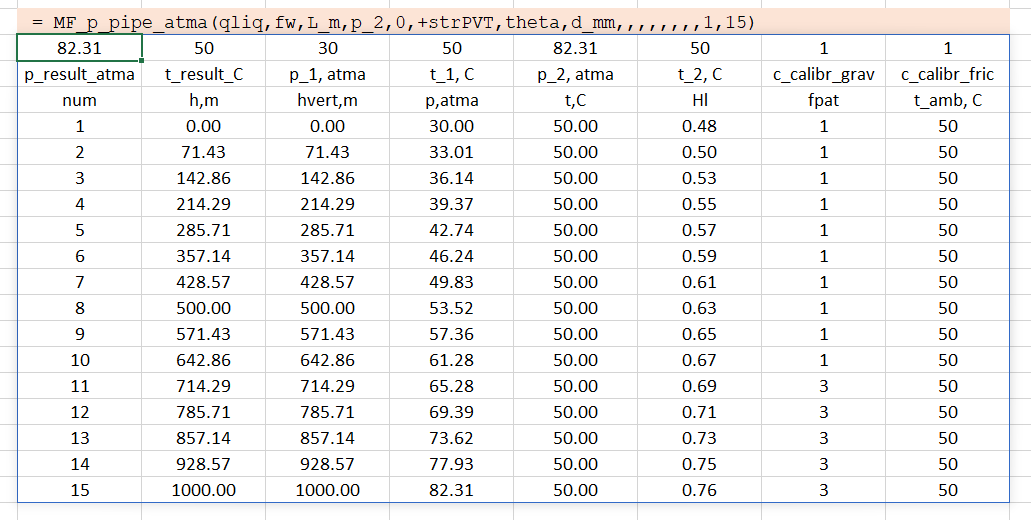
\includegraphics[width=1\linewidth]{pipe_out_example}}
	\caption{Пример вывода результатов расчета функции \mintinline{vb.net}{MF_p_pipe_atma()} для  \mintinline{vb.net}{out_curves=True} }
	\label{ris:pipe_out_example}
\end{figure}

\begin{figure}[ht]
	\center{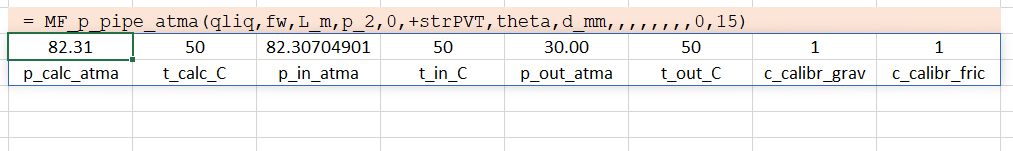
\includegraphics[width=1\linewidth]{pipe_out_example_short}}
	\caption{Пример вывода результатов расчета функции \mintinline{vb.net}{MF_p_pipe_atma()} для  \mintinline{vb.net}{out_curves=False} }
	\label{ris:pipe_out_example_short}
\end{figure}

\subsection{MF\_calibr\_pipe, MF\_calibr\_pipeline - функция калибровки расчета участка трубы}

Функция калибровки позволяет настроить модель потока в трубе под замеры давления на концах трубы. Настройка может проводиться за счет подбора различных параметров. Тип калибровки выбирается параметром \mintinline{vb.net}{calibr_type} В текущей реализации может быть подобран только один из перечисленных ниже параметров.

\begin{itemize}
	\item \mintinline{vb.net}{calibr_type=0} Калибровочный коэффициент многофазной корреляции для гравитационной составляющей  $c_{calibr\_grav}$. Ищется в диапазоне от 0.5 до 1.5.
	\item \mintinline{vb.net}{calibr_type=1} Калибровочный коэффициент многофазной корреляции для трения $c_{calibr\_fric}$. Ищется в диапазоне от 0.5 до 1.5.
	\item \mintinline{vb.net}{calibr_type=2} Газовый фактор $R_p$. Ищется в диапазоне $[20, 2 R_p]$ относительно заданного газового фактора. 
	\item \mintinline{vb.net}{calibr_type=3} Обводненность $f_w$.  Ищется в диапазоне $[0, 1]$.  
	\item \mintinline{vb.net}{calibr_type=4} Дебит жидкости \(Q_{liq} \). Ищется в диапазоне от \([0,Q_{liq}*1.5 ]\) относительно заданного дебита жидкости. 	 
	\item \mintinline{vb.net}{calibr_type=5} Дебит жидкости \(Q_{gas} \). Ищется в диапазоне от \([0,Q_{gas}*2 ]\) относительно заданного дебита газа или в диапазоне \([0,10000 ]\) м$^3$/сут если дебит газа не задан. 	
\end{itemize}

Результат расчета - массив с подобранным параметром или сообщением о невозможности подбора, информацией о количестве итераций. 

\putlisting{listings/MF_calibr_pipe.lst}

Подбор параметра может быть осуществлен для трубопровода, в котором может быть учтен профиль и более сложная температурная модель.

\putlisting{listings/MF_calibr_pipeline.lst}



\subsection{MF\_dpdl\_atmm – функция расчета градиента давления по многофазной корреляции Ансари}  
Иногда бывает удобно/интересно посмотреть детально на результаты расчета по многофазной корреляции. Для этого можно воспользоваться данной функцией. Внимательно смотрите описание и саму функцию. Выводит ряд параметров в массиве.
\putlisting{listings/MF_dpdl_atmm.lst}

\subsection{MF\_p\_pipeline\_atma - функция расчета трубопровода с учетом профиля и температуры}

Функция расчета трубопровода \mintinline{vb.net}{MF_p_pipeline_atma()} аналогична по функциональности функции расчета сегмента трубы \mintinline{vb.net}{MF_p_pipe_atma()} за исключением следующих моментов: в трубопроводе имеется возможность учета профиля трубопровода (инклинометрии для труб в скважине), возможность учета изменения диаметров для различных участков трубопровода и возможность более детального расчета распределения температуры флюида вдоль трубопровода (скважины) для некоторых конфигураций. Также для трубопровода всегда выводятся значения параметров потока между концами трубопровода в выходном массиве, в то время для трубы такой вывод можно подавить.

Функция отличается достаточно сложным поведением из-за возможности задания параметров в различных форматах. Данное описание не претендует на полноту. Рекомендуется изучать поведение функции на примерах. Тем не менее некоторые особенности параметров функции описаны ниже.

\begin{itemize}
	\item Параметр 	\mintinline{vb.net}{h_list_m} определяет траекторию скважины или трубопровода. Если задано одно число (или ссылка на ячейку с числом) то оно определяет длину трубопровода. Если задан двумерный массив (или ссылка на range) содержащий измеренные и вертикальные глубины, то задается траектория трубы/скважины. 
	\item Параметр 	\mintinline{vb.net}{diam_list_mm} определяет внутренний диаметр скважины или трубопровода. Если задано одно число (или ссылка на ячейку с числом) то оно определяет единый диаметр для всего трубопровода. Если задан двумерный массив (или ссылка на range) содержащий измеренные глубины и значения диаметров, то задается составной трубопровод с участками разных диаметров. 
	\item Параметр \mintinline{vb.net}{t_val} задает распределение температуры в трубопроводе или в пространстве окружающем трубопровод или скважину. Предполагается, что распределение температуры зависит от вертикальной глубины (модель больше рассчитана на скважину). Задается в виде двумерного массива (или объекта range) вертикальных глубин и температур. Если задано одно число - то модель расчета температуры будет линейная вдоль измеренной длины, а само число определяет температуру на втором конце трубы. Если задан двумерный массив значений, то модель расчета температуры определяется параметром \mintinline{vb.net}{temp_method}
	\item Параметр \mintinline{vb.net}{temp_method} определяет метод расчета распределения температуры. Для \mintinline{vb.net}{temp_method=2} используется метод с учетом эмиссии тепла в окружающее пространство. В текущей версии \unf{} для этого метода регулировка параметров теплопередачи возможна только в коде VBA. Для корректировки необходимо задать параметры объекта класса  \mintinline{vb.net}{CAmbientFormation}. Для примера смотри конструктор класса  \mintinline{vb.net}{CAmbientFormation.Class_Initialize}
	
\end{itemize}


\putlisting{listings/MF_p_pipeline_atma.lst}

Результатом работы функции является массив, содержащий давления и температуру на концах трубы, калибровочные параметры, а также значения ряда параметров между концами трубопровода.

\begin{figure}[ht]
	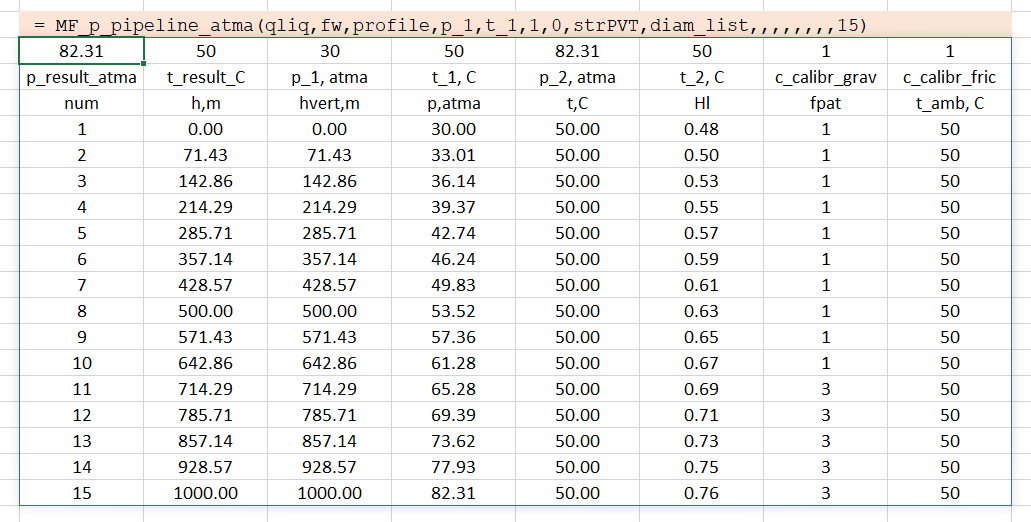
\includegraphics[width=1\linewidth]{pipeline_out_example}
	\caption{Пример вывода результатов расчета функции \mintinline{vb.net}{MF_p_pipeline_atma()}}
	\label{ris:pipeline_out_example}
\end{figure}
\end{comment}

\newpage

        % Глава многофазный поток
%	
\section{Расчет многофазного потока в пласте}
Для анализа работы скважины и скважинного оборудования в большинстве случаев достаточно простейшего подхода для описания производительности пласта. На текущий момент в \unf{} используется линейная индикаторная кривая с поправкой Вогеля для учета разгазирования в призабойной зоне пласта с учетом обводненности \cite{KBrown_AL_methods_vol4}. 

Пользовательские функции для расчета производительности пласта начинаются с префикса  \mintinline{vb.net}{IPR_}. 

Для расчета притока из пласта необходимо определить связь между дебитом жидкости $Q_{liq}$ (притоком) и забойным давлением работающей скважины $P_{wf}$.
Линейная индикаторная кривая на основе закона Дарси задает такую связь через коэффициент продуктивности скважины, который определяется как 
\begin{equation}\label{PI_def} 
 PI = \frac{Q_{liq}}{P_{res} - P_{wf}} 
\end{equation}

где $P_{res}$ - пластовое давление - давление на контуре питания скважины. Закон Дарси описывает установившийся приток несжимаемой жидкости в однородном пласте. 

Соответственно уравнение притока будет иметь вид

$$ Q_{liq} = PI \left( P_{res} - P_{wf} \right) $$

Для линейного притока по закону Дарси коэффициент продуктивности может быть оценен либо по данным эксплуатации из уравнения \ref{PI_def} либо по аналитической зависимости по характеристикам пласта и системы заканчивания. Например для радиального притока к вертикальной скважине широко известна формула Дюпюи согласно которой 
\begin{equation}\label{eq_Dupui} 
PI = f \cdot \frac{kh}{\mu B}\frac{1}{ \ln \dfrac{r_e}{r_w} + S }  
\end{equation}

здесь $f$ - размерный коэффициент, зависящий от выбранной системы единиц для остальных параметров. Так для системы единиц

\newcommand{\rnttab}[1]{
	\begin{tabular}[c]{@{}c@{}}#1\end{tabular}	
}

\begin{table}[H]
	\centering
	\caption{Размерности параметров выражения \ref{eq_Dupui}} \label{tab:dim_Dupui}
	\begin{tabular}{|c|c|c|c|c|}
		\hline
		Обозначение & Параметр   			        	& СИ           & \rnttab{Практические \\ метрические}     & \rnttab{Американские\\ промысловые} \\ \hline
		$f$        & \rnttab{размерный \\ коэффициент} & $2\pi$       & $\dfrac{1}{18.41}$     			      & $\dfrac{1}{141.2}$                      \\ \hline
		$k$        & проницаемость           		    & $\text{м}^2$ & мД                    					  & mD   							    \\ \hline
		$h$        & \rnttab{мощность \\ пласта}       & м            & м                      				  & ft   								    \\ \hline		
		$B$        & \rnttab{объемный \\ коэффициент}  & $\text{м}^3/\text{м}^3$    & $\text{м}^3/\text{м}^3$    & $scf/bbl$    						\\ \hline
		$\mu$      & вязкость                           & Па $\cdot$ с & сП                                       & сP                                  \\ \hline
		$r_e$      & \rnttab{радиус зоны \\ дренирования} & м & м                                       & ft                                  \\ \hline
		$r_w$      & \rnttab{радиус  \\ скважины} & м & м                                       & ft                                  \\ \hline
		$S$        & скин фактор 				   & \multicolumn{3}{c|}{безразмерный}                     \\ \hline
	\end{tabular}
\end{table}
 
 При снижении забойного давления добывающей скважины ниже давления насыщения, оценка дебита жидкости по закону Дарси  оказывается завышенной. Газ выделяющийся в призабойной зоне пласта создает дополнительное гидравлическое сопротивление.  В \unf{} поправка на снижение забойного давления ниже давления насыщения реализована на основе поправки Вогеля. Для безводной нефти по Вогелю продуктивность скважины по данным тестовой эксплуатации - дебите жидкости $Q_{liq}$ и соответствующем забойном давлении $P_{wf}$ может быть оценен по выражению \ref{eq_Vogel}.
 
 \begin{equation}\label{eq_Vogel} 
 PI = \frac{Q_{liq}}{P_{res} - P_{b} + \dfrac{P_{b}}{1.8} \left[ 1.0 - 0.2  \dfrac{P_{wf}}{P_{b}}- 0.8 \left( \dfrac{P_{wf}}{P_{b}} \right)^2 \right] }   
 \end{equation}
 
 При наличии обводненности зависимость усложняется.
 
 В \unf{} реализована модель определения коэффициента продуктивности по данным эксплуатации. Сравнение индикаторных кривых, построенных по тестовым данным $Q_{liq} = 100$ и $P_{wf} = 150$ при наличии и отсутствии воды, приведено на рисунке \ref{ris:IPR_curves}. 
 
 \begin{figure}[H]
 	\begin{center}
		 \newcommand{\IPRFile}{data/IPR_fw_data.txt}
		 \begin{tikzpicture}[scale=1]
		 \begin{axis}[
		 width=14cm,
		 height=10cm,
		 xlabel={$Q, m^3 / day$},
		 ylabel={$P_{wf},  atma$},
		 legend pos=north east,
		 title= Индикаторные кривые IPR]
		 \addplot table [y=Pwf_fw0, x=Q_fw0]{\IPRFile};
		 \addlegendentry{$f_w = 0$}
		 \addplot table [y=Pwf_fw95, x=Q_fw95]{\IPRFile};
		\addlegendentry{$f_w = 95$}
		 \end{axis}
		 \end{tikzpicture}
 	\caption{Сравнение индикаторных кривых для заданных тестовых параметров $Q_{liq} = 100$ и $P_{wf} = 150$ при наличии и отсутствии воды в потоке }
 \label{ris:IPR_curves}
\end{center}
\end{figure}
 

\subsection{IPR\_pi\_sm3dayatm – расчёт продуктивности}
Функция позволяет рассчитать коэффициент продуктивности скважины по данным тестовой эксплуатации. Особенность линейной модели притока к скважине с поправкой Вогеля заключается в минимальном наборе исходных данных, необходимых для построения индикаторной кривой. Достаточно знать пластовое давление, дебит и забойное давление в одной точке.

\putlisting{listings/IPR_PI_sm3dayatm.lst}


\subsection{IPR\_pwf\_atm – расчёт забойного давления по дебиту и продуктивности}
Функция позволяет рассчитать забойное давление скважины по известным значениям дебита и продуктивности.

\putlisting{listings/IPR_Pwf_atma.lst}

\subsection{IPR\_qliq\_sm3day – расчёт дебита по забойному давлению и продуктивности}
Функция позволяет рассчитать дебит жидкости скважины на поверхности по забойному давлению и продуктивности.

\putlisting{listings/IPR_Qliq_sm3Day.lst}



\newpage
       % Глава индикаторная кривая
%	\section{Расчёт УЭЦН}
Пользовательские функции, связанные с расчётом установок электрических центробежных насосов приведены в модуле «u7\_Excel\_functions\_ESP».  Названия функций начинаются с префикса \mintinline{vb.net}{ESP_}. 

\begin{figure}[H]
	\begin{center}
		

\tikzset{every picture/.style={line width=0.75pt}} %set default line width to 0.75pt        

\begin{tikzpicture}[x=0.75pt,y=0.75pt,yscale=-1,xscale=1]
%uncomment if require: \path (0,559); %set diagram left start at 0, and has height of 559

%Shape: Rectangle [id:dp9980881958960581] 
\draw  [fill={rgb, 255:red, 184; green, 233; blue, 134 }  ,fill opacity=1 ] (208.84,188.87) -- (235.84,188.87) -- (235.84,345.37) -- (208.84,345.37) -- cycle ;
%Shape: Rectangle [id:dp5932777464879899] 
\draw  [line width=2.25]  (186.87,95) -- (257.53,95) -- (257.53,524.67) -- (186.87,524.67) -- cycle ;
%Shape: Rectangle [id:dp479514803237743] 
\draw  [fill={rgb, 255:red, 184; green, 233; blue, 134 }  ,fill opacity=1 ] (209.78,348.7) -- (234.89,348.7) -- (234.89,403.2) -- (209.78,403.2) -- cycle ;
%Shape: Rectangle [id:dp4846107383227307] 
\draw  [fill={rgb, 255:red, 255; green, 255; blue, 255 }  ,fill opacity=1 ][line width=0.75]  (213.44,386.83) -- (215.8,386.83) -- (215.8,395.17) -- (213.44,395.17) -- cycle ;
%Shape: Ellipse [id:dp06168892340659493] 
\draw  [fill={rgb, 255:red, 255; green, 255; blue, 255 }  ,fill opacity=1 ] (213.13,360.77) .. controls (213.57,359.22) and (214.39,358.87) .. (214.97,359.98) .. controls (215.55,361.1) and (215.66,363.25) .. (215.23,364.79) .. controls (214.79,366.34) and (213.97,366.69) .. (213.39,365.58) .. controls (212.82,364.47) and (212.7,362.31) .. (213.13,360.77) -- cycle ;
%Shape: Ellipse [id:dp30200309963657546] 
\draw  [fill={rgb, 255:red, 255; green, 255; blue, 255 }  ,fill opacity=1 ] (228.42,361.21) .. controls (228.86,359.66) and (229.68,359.31) .. (230.26,360.42) .. controls (230.83,361.53) and (230.95,363.69) .. (230.51,365.23) .. controls (230.08,366.78) and (229.26,367.13) .. (228.68,366.02) .. controls (228.1,364.9) and (227.99,362.75) .. (228.42,361.21) -- cycle ;
%Shape: Rectangle [id:dp5532658444773444] 
\draw  [fill={rgb, 255:red, 74; green, 144; blue, 226 }  ,fill opacity=1 ] (206.34,437.26) -- (238.34,437.26) -- (238.34,506.76) -- (206.34,506.76) -- cycle ;
%Shape: Rectangle [id:dp30094154904153814] 
\draw  [fill={rgb, 255:red, 184; green, 233; blue, 134 }  ,fill opacity=1 ] (214.2,71) -- (230.2,71) -- (230.2,187.5) -- (214.2,187.5) -- cycle ;
%Shape: Rectangle [id:dp7288534663825625] 
\draw  [fill={rgb, 255:red, 155; green, 155; blue, 155 }  ,fill opacity=1 ] (206.34,406.62) -- (238.34,406.62) -- (238.34,433.62) -- (206.34,433.62) -- cycle ;
%Shape: Rectangle [id:dp28079882264446754] 
\draw  [fill={rgb, 255:red, 74; green, 144; blue, 226 }  ,fill opacity=1 ] (230.2,68.4) -- (235,68.4) -- (235,186.8) -- (230.2,186.8) -- cycle ;
%Shape: Rectangle [id:dp07010051943359463] 
\draw  [fill={rgb, 255:red, 74; green, 144; blue, 226 }  ,fill opacity=1 ] (235.7,183.5) -- (240.2,183.5) -- (240.2,440.5) -- (235.7,440.5) -- cycle ;
%Shape: Cross [id:dp6696618653175197] 
\draw  [fill={rgb, 255:red, 184; green, 233; blue, 134 }  ,fill opacity=1 ] (214.34,41.6) -- (230.34,41.6) -- (230.34,48.17) -- (236.91,48.17) -- (236.91,64.43) -- (230.34,64.43) -- (230.34,71) -- (214.34,71) -- (214.34,64.43) -- (207.77,64.43) -- (207.77,48.17) -- (214.34,48.17) -- cycle ;
%Shape: Rectangle [id:dp5472439702607639] 
\draw  [fill={rgb, 255:red, 255; green, 255; blue, 255 }  ,fill opacity=1 ][line width=0.75]  (218.63,386.83) -- (221,386.83) -- (221,395.17) -- (218.63,395.17) -- cycle ;
%Shape: Rectangle [id:dp22683999015700818] 
\draw  [fill={rgb, 255:red, 255; green, 255; blue, 255 }  ,fill opacity=1 ][line width=0.75]  (228.64,386.83) -- (231,386.83) -- (231,395.17) -- (228.64,395.17) -- cycle ;
%Shape: Rectangle [id:dp30061890316174966] 
\draw  [fill={rgb, 255:red, 255; green, 255; blue, 255 }  ,fill opacity=1 ][line width=0.75]  (223.4,386.83) -- (225.76,386.83) -- (225.76,395.17) -- (223.4,395.17) -- cycle ;
%Shape: Rectangle [id:dp1507413934687598] 
\draw  [fill={rgb, 255:red, 184; green, 233; blue, 134 }  ,fill opacity=1 ] (118.6,48.13) -- (207.8,48.13) -- (207.8,64.47) -- (118.6,64.47) -- cycle ;
%Shape: Rectangle [id:dp7399991400929342] 
\draw  [fill={rgb, 255:red, 74; green, 144; blue, 226 }  ,fill opacity=1 ] (230.2,64.47) -- (345.1,64.47) -- (345.1,68.4) -- (230.2,68.4) -- cycle ;
%Snip Same Side Corner Rect [id:dp9075267452915747] 
\draw  [fill={rgb, 255:red, 74; green, 144; blue, 226 }  ,fill opacity=1 ] (345.33,49.7) -- (359.22,35.82) -- (371.12,35.82) -- (385,49.7) -- (385,95) -- (385,95) -- (345.33,95) -- (345.33,95) -- cycle ;
%Snip Same Side Corner Rect [id:dp40079166384299336] 
\draw  [fill={rgb, 255:red, 74; green, 144; blue, 226 }  ,fill opacity=1 ] (403.33,48.28) -- (417.22,34.4) -- (429.12,34.4) -- (443,48.28) -- (443,95) -- (443,95) -- (403.33,95) -- (403.33,95) -- cycle ;
%Shape: Rectangle [id:dp998951658161422] 
\draw  [fill={rgb, 255:red, 74; green, 144; blue, 226 }  ,fill opacity=1 ] (385.8,65.2) -- (403.4,65.2) -- (403.4,69.2) -- (385.8,69.2) -- cycle ;
%Straight Lines [id:da4981174939654558] 
\draw [line width=3]    (77.4,95) -- (453.4,95) ;
%Shape: Rectangle [id:dp18436049413585986] 
\draw  [color={rgb, 255:red, 255; green, 255; blue, 255 }  ,draw opacity=1 ][fill={rgb, 255:red, 255; green, 255; blue, 255 }  ,fill opacity=1 ] (141.48,515.29) -- (302.91,515.29) -- (302.91,543.33) -- (141.48,543.33) -- cycle ;
%Shape: Rectangle [id:dp30389725435487924] 
\draw  [color={rgb, 255:red, 255; green, 255; blue, 255 }  ,draw opacity=1 ][fill={rgb, 255:red, 255; green, 255; blue, 255 }  ,fill opacity=1 ] (64.34,31.97) -- (125.57,31.97) -- (125.57,112) -- (64.34,112) -- cycle ;
%Flowchart: Punched Tape [id:dp7676649781733249] 
\draw  [color={rgb, 255:red, 255; green, 255; blue, 255 }  ,draw opacity=1 ][fill={rgb, 255:red, 255; green, 255; blue, 255 }  ,fill opacity=1 ] (170.95,128.75) .. controls (170.95,129.83) and (182.42,130.7) .. (196.57,130.7) .. controls (210.73,130.7) and (222.2,129.83) .. (222.2,128.75) .. controls (222.2,127.67) and (233.67,126.8) .. (247.82,126.8) .. controls (261.98,126.8) and (273.45,127.67) .. (273.45,128.75) -- (273.45,144.35) .. controls (273.45,143.27) and (261.98,142.4) .. (247.82,142.4) .. controls (233.67,142.4) and (222.2,143.27) .. (222.2,144.35) .. controls (222.2,145.43) and (210.73,146.3) .. (196.57,146.3) .. controls (182.42,146.3) and (170.95,145.43) .. (170.95,144.35) -- cycle ;
%Curve Lines [id:da8645149257470108] 
\draw    (173.45,144.35) .. controls (220,152) and (223,137.5) .. (273.45,144.35) ;
%Curve Lines [id:da6343227401532994] 
\draw    (173.45,128.75) .. controls (220,136.4) and (223,121.9) .. (273.45,128.75) ;
%Shape: Rectangle [id:dp3476162270559999] 
\draw  [color={rgb, 255:red, 155; green, 155; blue, 155 }  ,draw opacity=1 ][fill={rgb, 255:red, 74; green, 74; blue, 74 }  ,fill opacity=0.3 ] (220.44,192) -- (224.24,192) -- (224.24,505) -- (220.44,505) -- cycle ;
%Shape: Ellipse [id:dp861446695677758] 
\draw  [fill={rgb, 255:red, 255; green, 255; blue, 255 }  ,fill opacity=1 ] (221.29,360.99) .. controls (221.73,359.44) and (222.55,359.09) .. (223.13,360.2) .. controls (223.7,361.31) and (223.82,363.47) .. (223.39,365.01) .. controls (222.95,366.56) and (222.13,366.91) .. (221.55,365.8) .. controls (220.97,364.69) and (220.86,362.53) .. (221.29,360.99) -- cycle ;

% Text Node
\draw (278.7,454.7) node [anchor=north west][inner sep=0.75pt]   [align=left] {ПЭД};
% Text Node
\draw (274.8,412.62) node [anchor=north west][inner sep=0.75pt]   [align=left] {Гидрозащита};
% Text Node
\draw (277.5,365.83) node [anchor=north west][inner sep=0.75pt]   [align=left] {ГС};
% Text Node
\draw (280,266.83) node [anchor=north west][inner sep=0.75pt]   [align=left] {ЦН};
% Text Node
\draw (278,156.83) node [anchor=north west][inner sep=0.75pt]   [align=left] {Кабель};
% Text Node
\draw (356,58.33) node [anchor=north west][inner sep=0.75pt]   [align=left] {ТР};
% Text Node
\draw (412,59.83) node [anchor=north west][inner sep=0.75pt]   [align=left] {СУ};
% Text Node
\draw (208.84,508.01) node [anchor=north west][inner sep=0.75pt]   [align=left] {вал};
% Text Node
\draw (281,105.3) node [anchor=north west][inner sep=0.75pt]   [align=left] {НКТ};


\end{tikzpicture}
		\caption{Схема конструктивных элементов ЭЦН}
		\label{ris:ESP_well_1}
	\end{center}
\end{figure}

УЭЦН состоит из следующих основных конструктивных элементов:
\begin{itemize}
	\item ЦН -- центробежный насос. Модуль обеспечивающий перекачку жидкости за счёт преобразования механической энергии вращения вала в гидравлическую мощность. 
	\item ПЭД -- погружной электрический двигатель. Модуль обеспечивающий преобразование электрической энергии, поступающей по кабелю к погружному электрическому двигателю в механическую энергию вращения вала.
	\item ГС -- газосепаратор или приёмный модуль. Модуль обеспечивающий забор пластовой жидкости из скважины и подачу ее в насос. При этом центробежный газосепаратор способен отделить часть свободного газа в потоке и направить его в межтрубное пространство скважины. Работает за счёт механической энергии вращения вала.
	\item вал -- узел передающий энергию от погружного электрического двигателя (ПЭД) к остальным узлам установки, в том числе к центробежному насосу.
	\item кабель - узел передающий электрическую энергию с поверхности к погружному электрическому двигателю
	\item НКТ - колонна насосно компрессорных труб, на которой подвешен насос
	\item ТР -- трансформатор -- узел обеспечивающий необходимое напряжение на кабеле на поверхности. Как правило на вход трансформатора подается напряжение 380 В, а на выходе оно поднимается до нескольких тысяч вольт. 
	\item СУ -- станция управления ЭЦН. Узел управляющий работой системы УЭЦН. Может запускать и  останавливать скважины, обеспечивает защиту установки ЭЦН при нежелательных режимах работы
	\item ЧРП -- частотно регулируемый привод. Обычно комплектуется со станцией управления УЭЦН. Обеспечивает изменение частоты колебаний напряжения и тока, а соответственно и частоты вращения вала ЭЦН. Может отсутствовать в компоновке УЭЦН. 
\end{itemize}

Элементы показаны на рисунке \ref{ris:ESP_well_1} где гидравлическая часть и электрическая обозначены разными цветами.

В промысловых сводках и отчётах часто ЭЦН обозначаются с использованием значений габарита насоса, номинальной подачи и номинального напора. ЭЦН5А 50 - 2000, означает что, это насос 5А габарита, с номинальной подачей 50 м3/сут и напором 2000 м. 

\begin{figure}[H]
	\center{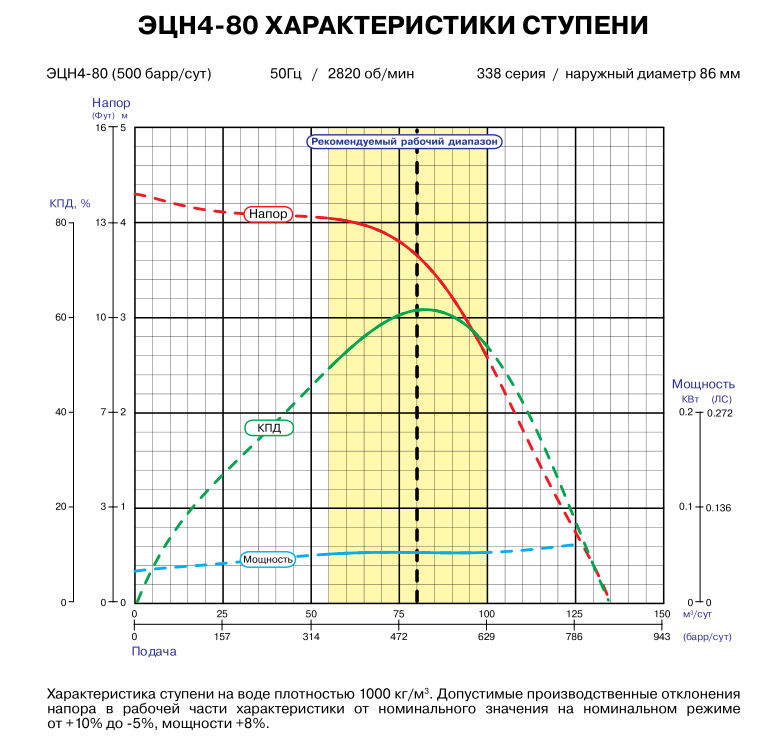
\includegraphics[width=0.8\linewidth]{novomet_ESP_80}}
	\caption{Пример каталожных характеристик ЭЦН}
	\label{ris:novomet_ESP_80}
\end{figure}

УЭЦН, как и другие центробежные машины, обладает относительно узким диапазоном подач при которых достигается достаточно высокий КПД его работы (от 30 до 60\%). В связи с этим для различных подач выпускаются различные типы УЭЦН. Всего в промышленности используются сотни различных типов ЭЦН различных производителей. Характеристики различных насосов предоставляются производителями в каталогах оборудования и обычно встраиваются в расчётные программы в виде баз данных характеристик оборудования. В надстройке \unf{} содержится база данных характеристик ЭЦН, которая может быть использована при проведении расчетов пользовательскими функциями. База сокращенная, содержит ряд насосов только одного производителя. Как правило этого достаточно для проведения базовых расчетов, так как характеристики насосов одного типоразмера разных производителей схожи между собой. 

Для выбора определённого насоса из базы необходимо использовать его идентификатор в базе - \mintinline{vb.net}{pump_id}

\begin{figure}[H]
	\begin{center}
		

\tikzset{every picture/.style={line width=0.75pt}} %set default line width to 0.75pt        

\begin{tikzpicture}[x=0.75pt,y=0.75pt,yscale=-1,xscale=1]
%uncomment if require: \path (0,547); %set diagram left start at 0, and has height of 547

%Shape: Rectangle [id:dp43797743969363] 
\draw  [fill={rgb, 255:red, 184; green, 233; blue, 134 }  ,fill opacity=1 ] (266.84,183.53) -- (293.84,183.53) -- (293.84,340.03) -- (266.84,340.03) -- cycle ;
%Shape: Rectangle [id:dp47794216093304787] 
\draw  [line width=2.25]  (244.87,89.67) -- (315.53,89.67) -- (315.53,519.33) -- (244.87,519.33) -- cycle ;
%Shape: Rectangle [id:dp694575277874794] 
\draw  [fill={rgb, 255:red, 184; green, 233; blue, 134 }  ,fill opacity=1 ] (267.78,343.37) -- (292.89,343.37) -- (292.89,397.87) -- (267.78,397.87) -- cycle ;
%Shape: Rectangle [id:dp17016886175690282] 
\draw  [fill={rgb, 255:red, 255; green, 255; blue, 255 }  ,fill opacity=1 ][line width=0.75]  (271.44,381.5) -- (273.8,381.5) -- (273.8,389.84) -- (271.44,389.84) -- cycle ;
%Shape: Ellipse [id:dp4236017419878271] 
\draw  [fill={rgb, 255:red, 255; green, 255; blue, 255 }  ,fill opacity=1 ] (271.13,355.43) .. controls (271.57,353.89) and (272.39,353.54) .. (272.97,354.65) .. controls (273.55,355.76) and (273.66,357.92) .. (273.23,359.46) .. controls (272.79,361.01) and (271.97,361.36) .. (271.39,360.25) .. controls (270.82,359.13) and (270.7,356.98) .. (271.13,355.43) -- cycle ;
%Shape: Ellipse [id:dp22440117531277237] 
\draw  [fill={rgb, 255:red, 255; green, 255; blue, 255 }  ,fill opacity=1 ] (286.42,355.87) .. controls (286.86,354.33) and (287.68,353.98) .. (288.26,355.09) .. controls (288.83,356.2) and (288.95,358.35) .. (288.51,359.9) .. controls (288.08,361.44) and (287.26,361.8) .. (286.68,360.68) .. controls (286.1,359.57) and (285.99,357.42) .. (286.42,355.87) -- cycle ;
%Shape: Rectangle [id:dp2759808393420238] 
\draw  [fill={rgb, 255:red, 74; green, 144; blue, 226 }  ,fill opacity=1 ] (264.34,431.93) -- (296.34,431.93) -- (296.34,501.43) -- (264.34,501.43) -- cycle ;
%Shape: Rectangle [id:dp4718416962393033] 
\draw  [fill={rgb, 255:red, 184; green, 233; blue, 134 }  ,fill opacity=1 ] (272.2,65.67) -- (288.2,65.67) -- (288.2,182.17) -- (272.2,182.17) -- cycle ;
%Shape: Rectangle [id:dp2471331363343623] 
\draw  [fill={rgb, 255:red, 155; green, 155; blue, 155 }  ,fill opacity=1 ] (264.34,401.29) -- (296.34,401.29) -- (296.34,428.29) -- (264.34,428.29) -- cycle ;
%Shape: Rectangle [id:dp8050530597562813] 
\draw  [fill={rgb, 255:red, 74; green, 144; blue, 226 }  ,fill opacity=1 ] (288.2,63.07) -- (293,63.07) -- (293,181.47) -- (288.2,181.47) -- cycle ;
%Shape: Rectangle [id:dp9151520855175173] 
\draw  [fill={rgb, 255:red, 74; green, 144; blue, 226 }  ,fill opacity=1 ] (293.7,178.17) -- (298.2,178.17) -- (298.2,435.17) -- (293.7,435.17) -- cycle ;
%Shape: Cross [id:dp4379121457669555] 
\draw  [fill={rgb, 255:red, 184; green, 233; blue, 134 }  ,fill opacity=1 ] (272.34,36.27) -- (288.34,36.27) -- (288.34,42.84) -- (294.91,42.84) -- (294.91,59.09) -- (288.34,59.09) -- (288.34,65.67) -- (272.34,65.67) -- (272.34,59.09) -- (265.77,59.09) -- (265.77,42.84) -- (272.34,42.84) -- cycle ;
%Shape: Rectangle [id:dp8860070074688149] 
\draw  [fill={rgb, 255:red, 255; green, 255; blue, 255 }  ,fill opacity=1 ][line width=0.75]  (276.63,381.5) -- (279,381.5) -- (279,389.84) -- (276.63,389.84) -- cycle ;
%Shape: Rectangle [id:dp3459479558989256] 
\draw  [fill={rgb, 255:red, 255; green, 255; blue, 255 }  ,fill opacity=1 ][line width=0.75]  (286.64,381.5) -- (289,381.5) -- (289,389.84) -- (286.64,389.84) -- cycle ;
%Shape: Rectangle [id:dp6778982988538649] 
\draw  [fill={rgb, 255:red, 255; green, 255; blue, 255 }  ,fill opacity=1 ][line width=0.75]  (281.4,381.5) -- (283.76,381.5) -- (283.76,389.84) -- (281.4,389.84) -- cycle ;
%Shape: Rectangle [id:dp2956843071937696] 
\draw  [fill={rgb, 255:red, 184; green, 233; blue, 134 }  ,fill opacity=1 ] (176.6,42.8) -- (265.8,42.8) -- (265.8,59.13) -- (176.6,59.13) -- cycle ;
%Shape: Rectangle [id:dp028493509366651848] 
\draw  [fill={rgb, 255:red, 74; green, 144; blue, 226 }  ,fill opacity=1 ] (288.2,59.13) -- (403.1,59.13) -- (403.1,63.07) -- (288.2,63.07) -- cycle ;
%Snip Same Side Corner Rect [id:dp16730933179178487] 
\draw  [fill={rgb, 255:red, 74; green, 144; blue, 226 }  ,fill opacity=1 ] (403.33,44.37) -- (417.22,30.48) -- (429.12,30.48) -- (443,44.37) -- (443,89.67) -- (443,89.67) -- (403.33,89.67) -- (403.33,89.67) -- cycle ;
%Snip Same Side Corner Rect [id:dp960862141285421] 
\draw  [fill={rgb, 255:red, 74; green, 144; blue, 226 }  ,fill opacity=1 ] (461.33,42.95) -- (475.22,29.07) -- (487.12,29.07) -- (501,42.95) -- (501,89.67) -- (501,89.67) -- (461.33,89.67) -- (461.33,89.67) -- cycle ;
%Shape: Rectangle [id:dp6987946544752222] 
\draw  [fill={rgb, 255:red, 74; green, 144; blue, 226 }  ,fill opacity=1 ] (443.8,59.87) -- (461.4,59.87) -- (461.4,63.87) -- (443.8,63.87) -- cycle ;
%Straight Lines [id:da3464083819146775] 
\draw [line width=3]    (135.4,89.67) -- (511.4,89.67) ;
%Shape: Rectangle [id:dp013160218055517703] 
\draw  [color={rgb, 255:red, 255; green, 255; blue, 255 }  ,draw opacity=1 ][fill={rgb, 255:red, 255; green, 255; blue, 255 }  ,fill opacity=1 ] (199.48,509.95) -- (360.91,509.95) -- (360.91,538) -- (199.48,538) -- cycle ;
%Shape: Rectangle [id:dp8788494742696384] 
\draw  [color={rgb, 255:red, 255; green, 255; blue, 255 }  ,draw opacity=1 ][fill={rgb, 255:red, 255; green, 255; blue, 255 }  ,fill opacity=1 ] (122.34,26.63) -- (183.57,26.63) -- (183.57,106.67) -- (122.34,106.67) -- cycle ;
%Flowchart: Punched Tape [id:dp14293584563200135] 
\draw  [color={rgb, 255:red, 255; green, 255; blue, 255 }  ,draw opacity=1 ][fill={rgb, 255:red, 255; green, 255; blue, 255 }  ,fill opacity=1 ] (228.95,123.42) .. controls (228.95,124.49) and (240.42,125.37) .. (254.57,125.37) .. controls (268.73,125.37) and (280.2,124.49) .. (280.2,123.42) .. controls (280.2,122.34) and (291.67,121.47) .. (305.82,121.47) .. controls (319.98,121.47) and (331.45,122.34) .. (331.45,123.42) -- (331.45,139.02) .. controls (331.45,137.94) and (319.98,137.07) .. (305.82,137.07) .. controls (291.67,137.07) and (280.2,137.94) .. (280.2,139.02) .. controls (280.2,140.09) and (268.73,140.97) .. (254.57,140.97) .. controls (240.42,140.97) and (228.95,140.09) .. (228.95,139.02) -- cycle ;
%Curve Lines [id:da9422778139456416] 
\draw    (231.45,139.02) .. controls (278,146.67) and (281,132.17) .. (331.45,139.02) ;
%Curve Lines [id:da4455203598547133] 
\draw    (231.45,123.42) .. controls (278,131.07) and (281,116.57) .. (331.45,123.42) ;
%Shape: Rectangle [id:dp1918341751021142] 
\draw  [color={rgb, 255:red, 155; green, 155; blue, 155 }  ,draw opacity=1 ][fill={rgb, 255:red, 74; green, 74; blue, 74 }  ,fill opacity=0.3 ] (278.44,186.67) -- (282.24,186.67) -- (282.24,499.67) -- (278.44,499.67) -- cycle ;
%Shape: Ellipse [id:dp06332103309338089] 
\draw  [fill={rgb, 255:red, 255; green, 255; blue, 255 }  ,fill opacity=1 ] (279.29,355.65) .. controls (279.73,354.11) and (280.55,353.76) .. (281.13,354.87) .. controls (281.7,355.98) and (281.82,358.14) .. (281.39,359.68) .. controls (280.95,361.23) and (280.13,361.58) .. (279.55,360.46) .. controls (278.97,359.35) and (278.86,357.2) .. (279.29,355.65) -- cycle ;
%Flowchart: Collate [id:dp5491359801292692] 
\draw  [fill={rgb, 255:red, 255; green, 255; blue, 255 }  ,fill opacity=1 ] (212.03,34.88) -- (230.37,34.88) -- (212.03,69.05) -- (230.37,69.05) -- cycle ;
%Straight Lines [id:da16622894570586455] 
\draw  [dash pattern={on 4.5pt off 4.5pt}]  (294,183.53) -- (363.5,183.53) ;
%Straight Lines [id:da21923594953984682] 
\draw  [dash pattern={on 4.5pt off 4.5pt}]  (286.5,385.67) -- (356,385.67) ;
%Straight Lines [id:da8352751178949347] 
\draw    (346.65,183.53) -- (345.66,383.67) ;
\draw [shift={(345.65,385.67)}, rotate = 270.28] [color={rgb, 255:red, 0; green, 0; blue, 0 }  ][line width=0.75]    (10.93,-3.29) .. controls (6.95,-1.4) and (3.31,-0.3) .. (0,0) .. controls (3.31,0.3) and (6.95,1.4) .. (10.93,3.29)   ;

% Text Node
\draw (414,53) node [anchor=north west][inner sep=0.75pt]   [align=left] {ТР};
% Text Node
\draw (470,54.5) node [anchor=north west][inner sep=0.75pt]   [align=left] {СУ};
% Text Node
\draw (195.5,174.53) node [anchor=north west][inner sep=0.75pt]   [align=left] {$ P_{dis}$};
% Text Node
\draw (201,376.67) node [anchor=north west][inner sep=0.75pt]   [align=left] {$ P_{int}$};
% Text Node
\draw (354,274.53) node [anchor=north west][inner sep=0.75pt]   [align=left] {$ L_{pump}$};
% Text Node
\draw (354.5,40.17) node [anchor=north west][inner sep=0.75pt]   [align=left] {$ I$};
% Text Node
\draw (380.5,21.17) node [anchor=north west][inner sep=0.75pt]   [align=left] {$ U_{tr}$};
% Text Node
\draw (320.65,419.67) node [anchor=north west][inner sep=0.75pt]   [align=left] {$\displaystyle U_{mot}$};


\end{tikzpicture}
		\caption{Схема конструктивных элементов ЭЦН}
		\label{ris:ESP_well_2}
	\end{center}
\end{figure}


Задача расчёта УЭЦН обычно сводится к расчёту гидравлических и электрических характеристик ЭЦН, ключевые из которых показанных на рисунке \ref{ris:ESP_well_2}. Выделяют несколько режимов расчёта:
\begin{itemize}
	\item Прямая задача - по заданным значениям дебита жидкости скважины,  давлению на приеме, напряжению питания УЭЦН на поверхности найти давление на выкиде насоса, потребляемую электрическую мощность, потребляемый ток установки, КПД всей системы и отдельных узлов системы
	\item Обратная задача - по данным контроля параметров работы УЭЦН на поверхности - потребляемому току, напряжению питания частоте подаваемого напряжения, данным по конструкции УЭЦН и скважины найти дебит жидкости и обводнённость по скважине, давление на приёме и забойное давление.
	\item Задача узлового анализа - по данным конструкции скважины, параметров работы погружного оборудования оценить дебит по жидкости скважины при заданным параметрах работы УЭЦН или при их изменении. К этому типу задач относится задача подбора погружного оборудования для достижения заданных условий эксплуатации 
	
\end{itemize}

Для расчёта УЭЦН требуется рассчитать гидравлические параметры работы ЦН и электромеханические параметры ПЭД.

Более подробно про УЭЦН можно прочитать в книге Gabor Tacacs Electrical Submersible Pumps Manual \cite{Gabor_ESP}.

\subsection{База характеристик ЭЦН}
Для расчёта параметров работы УЭЦН необходимо иметь возможность работы с фактическими расходно напорными характеристиками различных типов ЭЦН. Такая возможность обеспечивается за счет наличия в составе \unf{} базы характеристик ЭЦН, которая находится в файле \mintinline{vb.net}{ESP_json.db}. Файл базы должен находиться рядом с надстройкой, название нельзя менять, оно жестко зашито в коде (актуально для версии 7.25).
Файл базы данных текстовый в формате \href{https://ru.wikipedia.org/wiki/JSON}{json}. Что обеспечивает достаточно простую работу с ним и потенциальную возможность внесения новых типов оборудования без привлечения внешних инструментов. Тем не менее в папке \mintinline{vb.net}{db/} репозитория можно найти вариант базы данных в формате Excel \mintinline{vb.net}{ESP_db.xlsm} с возможностью генерации json базы.    

\begin{figure}[H]
	\center{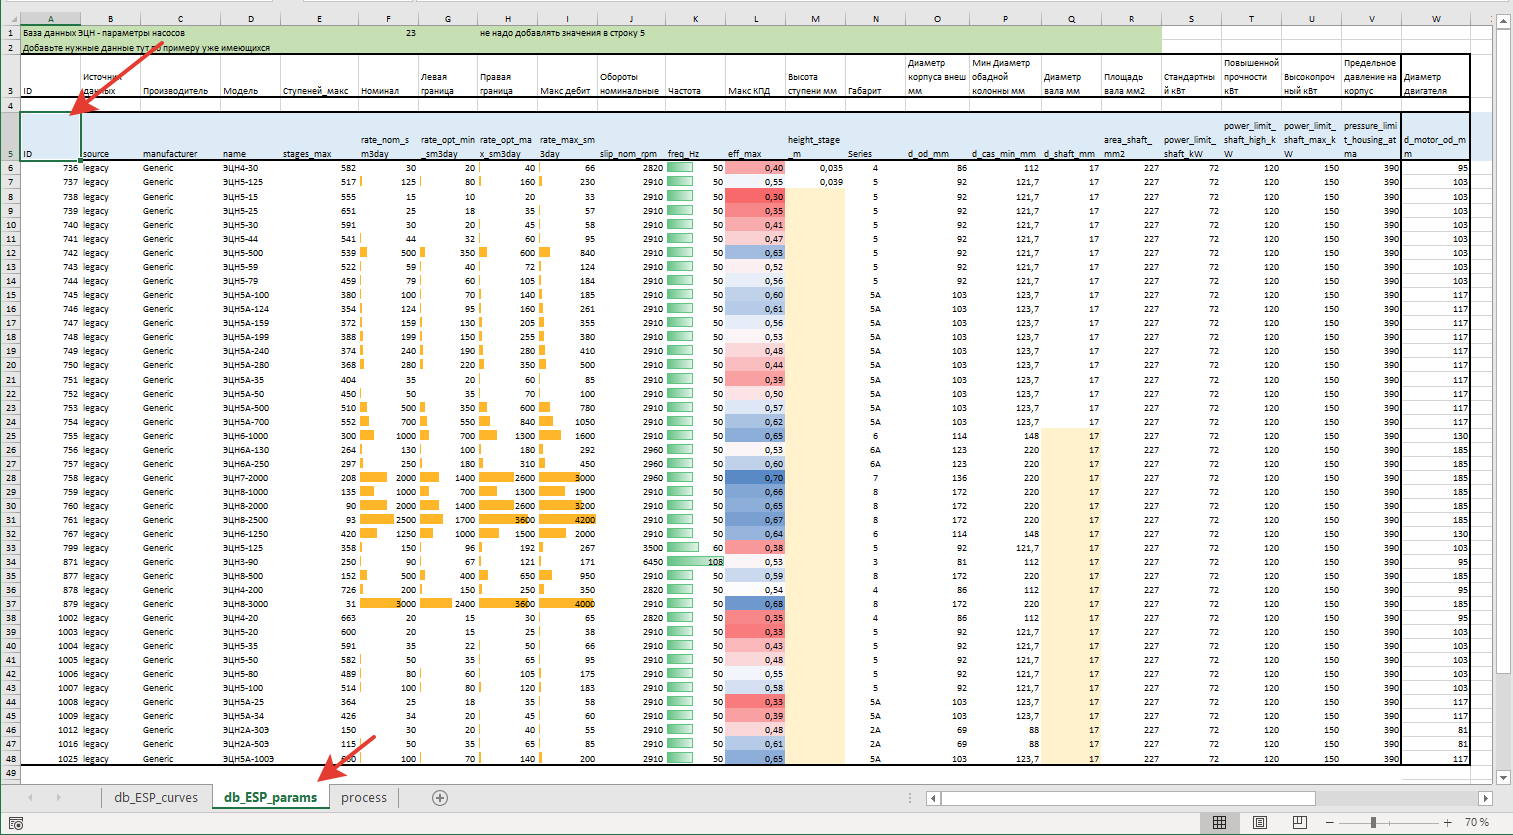
\includegraphics[width=1\linewidth]{ESP_db_1}}
	\caption{лист \mintinline{vb.net}{db_ESP_params} файла с базой ЭЦН}
	\label{ris:ESP_db_1}
\end{figure}

Файл \mintinline{vb.net}{ESP_db.xlsm} не зависит от надстройки \unf{} и может работать самостоятельно. База, фактически, состоит из двух таблиц на листах \mintinline{vb.net}{db_ESP_params} (смотри рисунок \ref{ris:ESP_db_1})  и \mintinline{vb.net}{db_ESP_curves} (смотри  рисунок \ref{ris:ESP_db_2}). Первая хранит параметры ЭЦН, вторая кривые расходно напорных характеристик. Таблицы связаны по идентификатору насоса \mintinline{vb.net}{ID}. Для добавления нового насоса следует добавить строку в таблицу на листе \mintinline{vb.net}{db_ESP_params} с соответствующими параметрами (все поля обязательны к заполнению) и добавить строки в таблицу \mintinline{vb.net}{db_ESP_curves} с тем же идентификатором \mintinline{vb.net}{ID} и значениями кривых РНХ (не менее 5 точек должно быть задано). При проведении расчётов кривые РНХ будут проинтерполированы кубическими сплайнами.  

\begin{figure}[H]
	\center{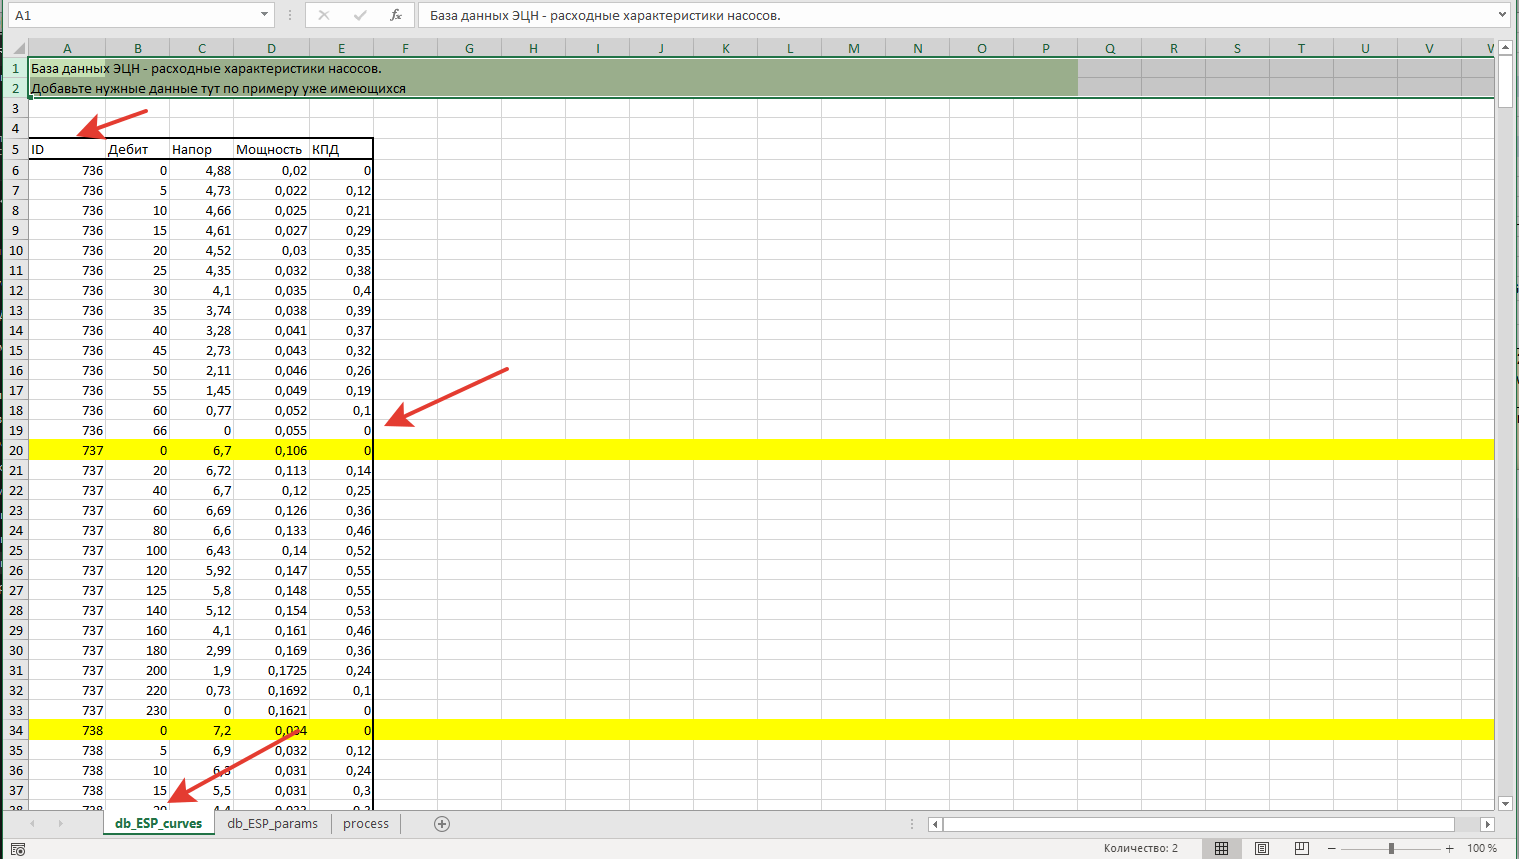
\includegraphics[width=1\linewidth]{ESP_db_2}}
	\caption{лист \mintinline{vb.net}{db_ESP_curves} файла с базой ЭЦН}
	\label{ris:ESP_db_2}
\end{figure}

Заголовки строки 5 на листе \mintinline{vb.net}{db_ESP_params} (смотри  рисунок \ref{ris:ESP_db_3}) определяют ключи параметров в json файле. Их нельзя менять, так как при считывании они жёстко зашиты в коде. Если в таблицу добавить столбец с новым названием, то он тоже будет записан в json файл, но не будет учитываться в расчётах без соответствующих модификаций в коде. Строка 4 должна быть пустой для корректной работы макроса (при считывании выделяется заполненная область вокруг левого верхнего угла таблицы - ячейки с названием \mintinline{vb.net}{db_ESP_params_topleft}).

\begin{figure}[H]
	\center{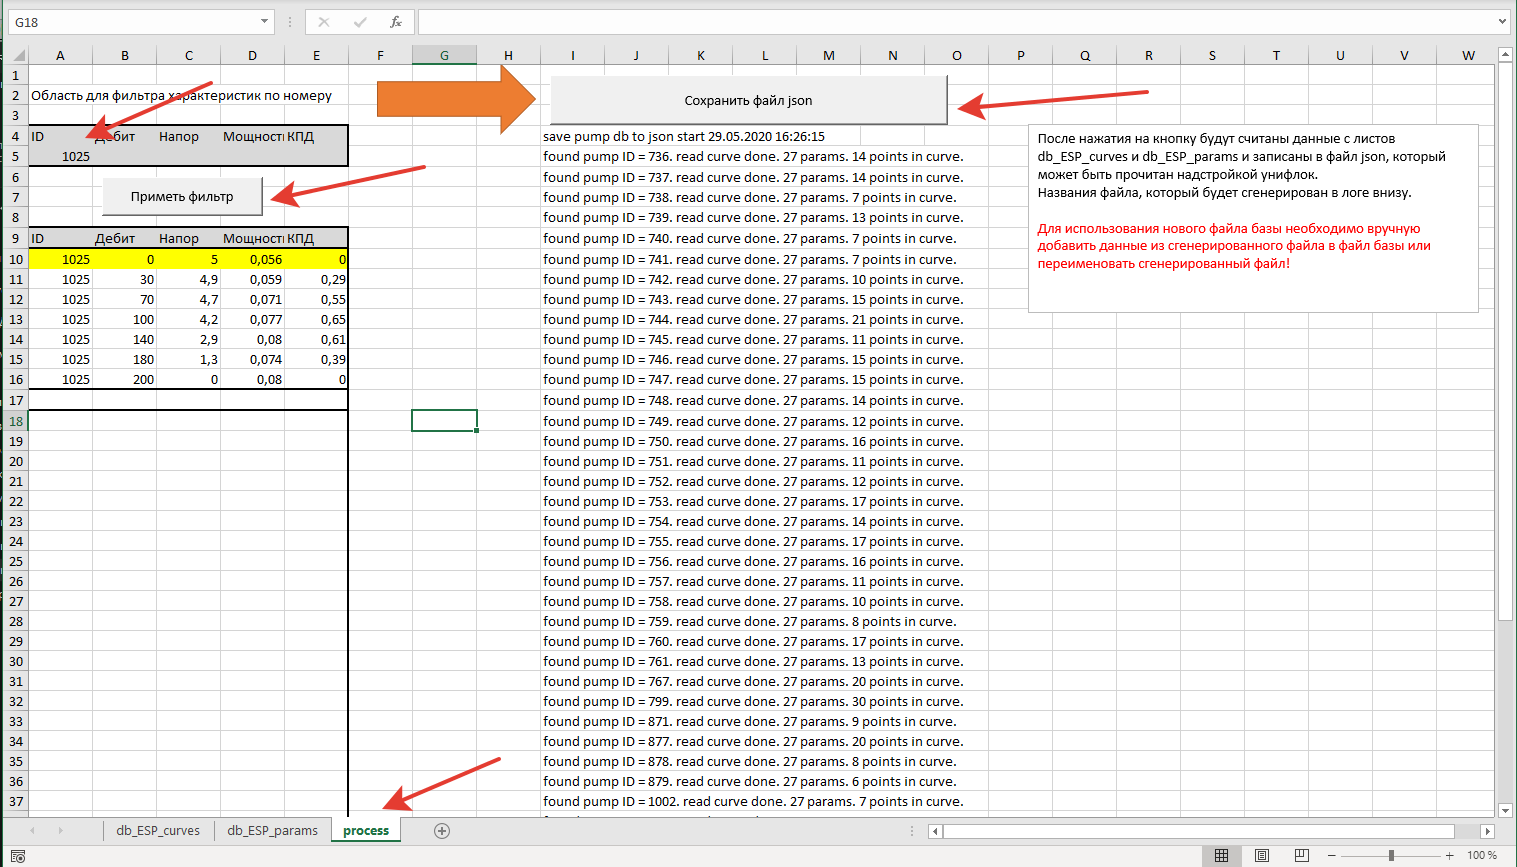
\includegraphics[width=1\linewidth]{ESP_db_3}}
	\caption{лист \mintinline{vb.net}{process} файла с базой ЭЦН}
	\label{ris:ESP_db_3}
\end{figure}

На листе \mintinline{vb.net}{process} таблицы есть возможность извлечь из базы расходно напорные характеристики одного насоса, а также сохранить файл в формате json. Для использования сгенерированного файла в \unf{} его потребуется вручную переименовать и переместить в папку с надстройкой \unf{}. 



\subsection{ESP\_head\_m – расчёт номинального напора ЭЦН}
Функция позволяет получить паспортные характеристики ЭЦН. Возвращает значение напора при определённой подаче. При указанном значении вязкости нефти пересчитывает паспортные характеристики с учётом вязкости.

\putlisting{listings/ESP_head_m.lst}

Расчёт выполняется на основе паспортных характеристик ЦН из каталога встроенного в надстройку \unf{}. 

\subsection{ESP\_eff\_fr – расчёт номинального КПД ЭЦН}
Функция позволяет получить паспортные характеристики ЭЦН. Возвращает значение КПД насоса при определённой подаче. При указанном значении вязкости нефти пересчитывает паспортные характеристики с учётом вязкости.

\putlisting{listings/ESP_eff_fr.lst}

Расчёт выполняется на основе паспортных характеристик ЦН из каталога встроенного в надстройку \unf{}. 

\subsection{ESP\_power\_W – расчёт номинальной мощности потребляемой ЭЦН}
Функция позволяет получить паспортные характеристики ЭЦН. Возвращает значение потребляемой с вала механической мощности при определённой подаче. При указанном значении вязкости нефти пересчитывает паспортные характеристики с учётом вязкости. 

\putlisting{listings/ESP_Power_W.lst}

Расчёт выполняется на основе паспортных характеристик ЦН из каталога встроенного в надстройку \unf{}. 

\subsection{ESP\_id\_by\_rate – выбор типового насоса по номинальному дебиту}
Функция возвращает идентификатор типового насоса по заданному номинальному дебиту. 
Может быть использована для выбора насоса на основе его наименования типа ЭЦН 50 - 2000.
\putlisting{listings/ESP_id_by_rate.lst}

\subsection{ESP\_p\_atma – расчёт распределения давления в ЭЦН}
Функция рассчитывает перепад давления, развиваемый ЦН при заданных параметрах флюида и термобарических условиях. Это одна из основных функция расчёта ЭЦН, комбинирующая характеристики из каталога и гидравлическую модель работы ЭЦН.
$$ P_{dis} = P_{int} + \sum_i^n{\rho_{mix,rc}(\bar{P}_{st,i},T) \cdot g \cdot h_{st,i}(Q_{mix,i}(\bar{P}_{st,i},T))} $$
где 
\begin{itemize}
	\item $P_{dis}$ - давление на выкиде насоса;
	\item $P_{int}$ - давление на приёме насоса;
	\item $i$ - номер ступени, или набора ступеней для ускоренного расчёта;
	\item $n$ - количество ступеней или наборов ступеней;
	\item $\bar{P}_{st,i}$ - среднее давление на  ступени $i$;
	\item $\rho_{mix,rc}$ - плотность ГЖС  в ступени $i$ ;
	\item $h_{st,i}$ - напор развиваемый  в ступени $i$;
	\item $Q_{mix,i}$ - расход ГЖС в ступени $i$;
	\item $g$ - ускорение свободного падения;
	
\end{itemize}


При расчёте сделаны следующие предположения:
\begin{itemize}
	\item не учитывается проскальзывание для асинхронного двигателя. Несмотря на то, что в базе может быть задана частота вращения с учётом проскальзывания, в этой функции считается, что \(slip = 0\) и ЦН вращается с частотой вращения электрического поля заданного параметром \mintinline{vb.net}{freq_Hz}. Для учета проскальзывания следует использовать функцию \mintinline{vb.net}{ESP_system_calc} или скорректировать частоту \mintinline{vb.net}{freq_Hz} вручную.
	\item в расчёте предполагается, что при повышении давления свободный газ растворится в нефти в соответствии с заданными PVT параметрами. Фактически работает опция - свободный газ растворяется. Для того, чтобы реализовать вариант расчёта при котором свободный газ при повышении давления не успеет раствориться в нефти следует модифицировать свойства флюида поступающего в насос так, чтобы запретить его растворение больше определённого предела (изменить давление насыщения $P_b$ и газосодержание при давлении насыщения $r_{sb}$)
	\item возможен как расчёт давления на выкиде по давлению на приёме, так и расчёт давления на приёме по давлению на выкиде (регулируется параметром \mintinline{vb.net}{calc_along_flow}). При этом расчёт ведётся непосредственным интегрированием по ступеням ЭЦН с шагом \mintinline{vb.net}{dnum_stages_integrate}). Расчёт против потока, при котором по давлению на выкиде рассчитывается давление на приёме следует применять с осторожностью. В этом варианте не сработают поправки на влияние газа, так как они предполагаю расчёт величины поправки от доли газа на приёме, которая не известна при старте расчёта. Кроме того при большом шаге интегрирования \mintinline{vb.net}{dnum_stages_integrate}) может накапливаться ошибка влияния газа при низких давлениях. Более надёжным вариантом расчёта давления на приёме по известному давлению на выкиде будет итеративный расчёт (подбор такого давления на приёме при котором будет обеспечиваться заданное давление на выкиде)
	\item температурный расчёт ЭЦН - расчёт температуры флюида на выкиде насоса - возможен только для варианта расчёта от давления на приёме к давлению на выкиде  \mintinline{vb.net}{calc_along_flow=True}). При этом не учитывается эмиссия тепла в окружающее пространство от корпуса насоса. Предполагается, что все выделившееся тепло идёт на нагрев флюида.
	
\end{itemize}

\putlisting{listings/ESP_p_atma.lst}
\begin{comment}
\subsection{ESP\_calibr\_pump – подбор подстроечных параметров ЭЦН}

Функция позволяет по известным значениям давления на приеме насоса и на выкиде насоса найти значения калибровочных параметров - калибровки по напору и по расходу. Ищется только одно значение калибровочного параметра.

%\putlisting{listings/ESP_calibr_pump.lst}


\subsection{Кодирование параметров ЭЦН в строке}
Для удобства работы с функциями учитывающими наличие ЭЦН в скважине созданы функции кодирования параметров УЭЦН в строке. Аналогично функциям кодирования PVT параметров, такие функции позволяют передать все необходимые данные о ЭЦН одним параметром.

Реализованы две функции - кодирования и декодирования строки ЭЦН.

%\putlisting{listings/ESP_pump_encode_string.lst}

%\putlisting{listings/ESP_motor_encode_string.lst}

%\putlisting{listings/ESP_cable_encode_string.lst}

%\putlisting{listings/ESP_separation_encode_string.lst}


\subsection{ESP\_system\_calc – расчет параметров работы УЭЦН}
Функция рассчитывает полный набор параметров работы УЭЦН при заданных параметрах флюида и термобарических условиях. В отличии от функции  \mintinline{vb.net}{ESP_p_atma} учитывает проскальзывание при расчете частоты вращения вала и рассчитывает электрические параметры работы ЭЦН.

\begin{figure}[H]
	\begin{center}
		

\tikzset{every picture/.style={line width=0.75pt}} %set default line width to 0.75pt        

\begin{tikzpicture}[x=0.75pt,y=0.75pt,yscale=-1,xscale=1]
%uncomment if require: \path (0,547); %set diagram left start at 0, and has height of 547

%Shape: Rectangle [id:dp43797743969363] 
\draw  [fill={rgb, 255:red, 184; green, 233; blue, 134 }  ,fill opacity=1 ] (266.84,183.53) -- (293.84,183.53) -- (293.84,340.03) -- (266.84,340.03) -- cycle ;
%Shape: Rectangle [id:dp47794216093304787] 
\draw  [line width=2.25]  (244.87,89.67) -- (315.53,89.67) -- (315.53,519.33) -- (244.87,519.33) -- cycle ;
%Shape: Rectangle [id:dp694575277874794] 
\draw  [fill={rgb, 255:red, 184; green, 233; blue, 134 }  ,fill opacity=1 ] (267.78,343.37) -- (292.89,343.37) -- (292.89,397.87) -- (267.78,397.87) -- cycle ;
%Shape: Rectangle [id:dp17016886175690282] 
\draw  [fill={rgb, 255:red, 255; green, 255; blue, 255 }  ,fill opacity=1 ][line width=0.75]  (271.44,381.5) -- (273.8,381.5) -- (273.8,389.84) -- (271.44,389.84) -- cycle ;
%Shape: Ellipse [id:dp4236017419878271] 
\draw  [fill={rgb, 255:red, 255; green, 255; blue, 255 }  ,fill opacity=1 ] (271.13,355.43) .. controls (271.57,353.89) and (272.39,353.54) .. (272.97,354.65) .. controls (273.55,355.76) and (273.66,357.92) .. (273.23,359.46) .. controls (272.79,361.01) and (271.97,361.36) .. (271.39,360.25) .. controls (270.82,359.13) and (270.7,356.98) .. (271.13,355.43) -- cycle ;
%Shape: Ellipse [id:dp22440117531277237] 
\draw  [fill={rgb, 255:red, 255; green, 255; blue, 255 }  ,fill opacity=1 ] (286.42,355.87) .. controls (286.86,354.33) and (287.68,353.98) .. (288.26,355.09) .. controls (288.83,356.2) and (288.95,358.35) .. (288.51,359.9) .. controls (288.08,361.44) and (287.26,361.8) .. (286.68,360.68) .. controls (286.1,359.57) and (285.99,357.42) .. (286.42,355.87) -- cycle ;
%Shape: Rectangle [id:dp2759808393420238] 
\draw  [fill={rgb, 255:red, 74; green, 144; blue, 226 }  ,fill opacity=1 ] (264.34,431.93) -- (296.34,431.93) -- (296.34,501.43) -- (264.34,501.43) -- cycle ;
%Shape: Rectangle [id:dp4718416962393033] 
\draw  [fill={rgb, 255:red, 184; green, 233; blue, 134 }  ,fill opacity=1 ] (272.2,65.67) -- (288.2,65.67) -- (288.2,182.17) -- (272.2,182.17) -- cycle ;
%Shape: Rectangle [id:dp2471331363343623] 
\draw  [fill={rgb, 255:red, 155; green, 155; blue, 155 }  ,fill opacity=1 ] (264.34,401.29) -- (296.34,401.29) -- (296.34,428.29) -- (264.34,428.29) -- cycle ;
%Shape: Rectangle [id:dp8050530597562813] 
\draw  [fill={rgb, 255:red, 74; green, 144; blue, 226 }  ,fill opacity=1 ] (288.2,63.07) -- (293,63.07) -- (293,181.47) -- (288.2,181.47) -- cycle ;
%Shape: Rectangle [id:dp9151520855175173] 
\draw  [fill={rgb, 255:red, 74; green, 144; blue, 226 }  ,fill opacity=1 ] (293.7,178.17) -- (298.2,178.17) -- (298.2,435.17) -- (293.7,435.17) -- cycle ;
%Shape: Cross [id:dp4379121457669555] 
\draw  [fill={rgb, 255:red, 184; green, 233; blue, 134 }  ,fill opacity=1 ] (272.34,36.27) -- (288.34,36.27) -- (288.34,42.84) -- (294.91,42.84) -- (294.91,59.09) -- (288.34,59.09) -- (288.34,65.67) -- (272.34,65.67) -- (272.34,59.09) -- (265.77,59.09) -- (265.77,42.84) -- (272.34,42.84) -- cycle ;
%Shape: Rectangle [id:dp8860070074688149] 
\draw  [fill={rgb, 255:red, 255; green, 255; blue, 255 }  ,fill opacity=1 ][line width=0.75]  (276.63,381.5) -- (279,381.5) -- (279,389.84) -- (276.63,389.84) -- cycle ;
%Shape: Rectangle [id:dp3459479558989256] 
\draw  [fill={rgb, 255:red, 255; green, 255; blue, 255 }  ,fill opacity=1 ][line width=0.75]  (286.64,381.5) -- (289,381.5) -- (289,389.84) -- (286.64,389.84) -- cycle ;
%Shape: Rectangle [id:dp6778982988538649] 
\draw  [fill={rgb, 255:red, 255; green, 255; blue, 255 }  ,fill opacity=1 ][line width=0.75]  (281.4,381.5) -- (283.76,381.5) -- (283.76,389.84) -- (281.4,389.84) -- cycle ;
%Shape: Rectangle [id:dp2956843071937696] 
\draw  [fill={rgb, 255:red, 184; green, 233; blue, 134 }  ,fill opacity=1 ] (176.6,42.8) -- (265.8,42.8) -- (265.8,59.13) -- (176.6,59.13) -- cycle ;
%Shape: Rectangle [id:dp028493509366651848] 
\draw  [fill={rgb, 255:red, 74; green, 144; blue, 226 }  ,fill opacity=1 ] (288.2,59.13) -- (403.1,59.13) -- (403.1,63.07) -- (288.2,63.07) -- cycle ;
%Snip Same Side Corner Rect [id:dp16730933179178487] 
\draw  [fill={rgb, 255:red, 74; green, 144; blue, 226 }  ,fill opacity=1 ] (403.33,44.37) -- (417.22,30.48) -- (429.12,30.48) -- (443,44.37) -- (443,89.67) -- (443,89.67) -- (403.33,89.67) -- (403.33,89.67) -- cycle ;
%Snip Same Side Corner Rect [id:dp960862141285421] 
\draw  [fill={rgb, 255:red, 74; green, 144; blue, 226 }  ,fill opacity=1 ] (461.33,42.95) -- (475.22,29.07) -- (487.12,29.07) -- (501,42.95) -- (501,89.67) -- (501,89.67) -- (461.33,89.67) -- (461.33,89.67) -- cycle ;
%Shape: Rectangle [id:dp6987946544752222] 
\draw  [fill={rgb, 255:red, 74; green, 144; blue, 226 }  ,fill opacity=1 ] (443.8,59.87) -- (461.4,59.87) -- (461.4,63.87) -- (443.8,63.87) -- cycle ;
%Straight Lines [id:da3464083819146775] 
\draw [line width=3]    (135.4,89.67) -- (511.4,89.67) ;
%Shape: Rectangle [id:dp013160218055517703] 
\draw  [color={rgb, 255:red, 255; green, 255; blue, 255 }  ,draw opacity=1 ][fill={rgb, 255:red, 255; green, 255; blue, 255 }  ,fill opacity=1 ] (199.48,509.95) -- (360.91,509.95) -- (360.91,538) -- (199.48,538) -- cycle ;
%Shape: Rectangle [id:dp8788494742696384] 
\draw  [color={rgb, 255:red, 255; green, 255; blue, 255 }  ,draw opacity=1 ][fill={rgb, 255:red, 255; green, 255; blue, 255 }  ,fill opacity=1 ] (122.34,26.63) -- (183.57,26.63) -- (183.57,106.67) -- (122.34,106.67) -- cycle ;
%Flowchart: Punched Tape [id:dp14293584563200135] 
\draw  [color={rgb, 255:red, 255; green, 255; blue, 255 }  ,draw opacity=1 ][fill={rgb, 255:red, 255; green, 255; blue, 255 }  ,fill opacity=1 ] (228.95,123.42) .. controls (228.95,124.49) and (240.42,125.37) .. (254.57,125.37) .. controls (268.73,125.37) and (280.2,124.49) .. (280.2,123.42) .. controls (280.2,122.34) and (291.67,121.47) .. (305.82,121.47) .. controls (319.98,121.47) and (331.45,122.34) .. (331.45,123.42) -- (331.45,139.02) .. controls (331.45,137.94) and (319.98,137.07) .. (305.82,137.07) .. controls (291.67,137.07) and (280.2,137.94) .. (280.2,139.02) .. controls (280.2,140.09) and (268.73,140.97) .. (254.57,140.97) .. controls (240.42,140.97) and (228.95,140.09) .. (228.95,139.02) -- cycle ;
%Curve Lines [id:da9422778139456416] 
\draw    (231.45,139.02) .. controls (278,146.67) and (281,132.17) .. (331.45,139.02) ;
%Curve Lines [id:da4455203598547133] 
\draw    (231.45,123.42) .. controls (278,131.07) and (281,116.57) .. (331.45,123.42) ;
%Shape: Rectangle [id:dp1918341751021142] 
\draw  [color={rgb, 255:red, 155; green, 155; blue, 155 }  ,draw opacity=1 ][fill={rgb, 255:red, 74; green, 74; blue, 74 }  ,fill opacity=0.3 ] (278.44,186.67) -- (282.24,186.67) -- (282.24,499.67) -- (278.44,499.67) -- cycle ;
%Shape: Ellipse [id:dp06332103309338089] 
\draw  [fill={rgb, 255:red, 255; green, 255; blue, 255 }  ,fill opacity=1 ] (279.29,355.65) .. controls (279.73,354.11) and (280.55,353.76) .. (281.13,354.87) .. controls (281.7,355.98) and (281.82,358.14) .. (281.39,359.68) .. controls (280.95,361.23) and (280.13,361.58) .. (279.55,360.46) .. controls (278.97,359.35) and (278.86,357.2) .. (279.29,355.65) -- cycle ;
%Flowchart: Collate [id:dp5491359801292692] 
\draw  [fill={rgb, 255:red, 255; green, 255; blue, 255 }  ,fill opacity=1 ] (212.03,34.88) -- (230.37,34.88) -- (212.03,69.05) -- (230.37,69.05) -- cycle ;
%Straight Lines [id:da16622894570586455] 
\draw  [dash pattern={on 4.5pt off 4.5pt}]  (294,183.53) -- (363.5,183.53) ;
%Straight Lines [id:da21923594953984682] 
\draw  [dash pattern={on 4.5pt off 4.5pt}]  (286.5,385.67) -- (356,385.67) ;
%Straight Lines [id:da8352751178949347] 
\draw    (346.65,183.53) -- (345.66,383.67) ;
\draw [shift={(345.65,385.67)}, rotate = 270.28] [color={rgb, 255:red, 0; green, 0; blue, 0 }  ][line width=0.75]    (10.93,-3.29) .. controls (6.95,-1.4) and (3.31,-0.3) .. (0,0) .. controls (3.31,0.3) and (6.95,1.4) .. (10.93,3.29)   ;

% Text Node
\draw (414,53) node [anchor=north west][inner sep=0.75pt]   [align=left] {ТР};
% Text Node
\draw (470,54.5) node [anchor=north west][inner sep=0.75pt]   [align=left] {СУ};
% Text Node
\draw (195.5,174.53) node [anchor=north west][inner sep=0.75pt]   [align=left] {$ P_{dis}$};
% Text Node
\draw (201,376.67) node [anchor=north west][inner sep=0.75pt]   [align=left] {$ P_{int}$};
% Text Node
\draw (354,274.53) node [anchor=north west][inner sep=0.75pt]   [align=left] {$ L_{pump}$};
% Text Node
\draw (354.5,40.17) node [anchor=north west][inner sep=0.75pt]   [align=left] {$ I$};
% Text Node
\draw (380.5,21.17) node [anchor=north west][inner sep=0.75pt]   [align=left] {$ U_{tr}$};
% Text Node
\draw (320.65,419.67) node [anchor=north west][inner sep=0.75pt]   [align=left] {$\displaystyle U_{mot}$};


\end{tikzpicture}
		\caption{Схема конструктивных элементов ЭЦН}
		\label{ris:ESP_well_2_1}
	\end{center}
\end{figure}


\putlisting{listings/ESP_system_calc.lst}


\subsection{Электромеханический расчёт погружного электрического двигателя ПЭД}
Рассматривается асинхронный электрический двигатель. 

Погружные асинхронные электрические двигатели для добычи нефти выполняются трехфазными. 

Впервые конструкция трёхфазного асинхронного двигателя была разработана, создана и опробована русским инженером М. О. Доливо-Добровольским в 1889-91 годах. Демонстрация первых двигателей состоялась на Международной электротехнической выставке во Франкфурте на Майне в сентябре 1891 года. Были представлены три трёхфазных двигателя разной мощности. Самый мощный из них имел мощность 1.5 кВт и использовался для приведения во вращение генератора постоянного тока. Конструкция асинхронного двигателя, предложенная Доливо-Добровольским, оказалась очень удачной и является основным видом конструкции этих двигателей до настоящего времени.

За прошедшие годы асинхронные двигатели нашли широкое применение в различных отраслях промышленности. Их используют в электроприводе металлорежущих станков, подъёмно-транспортных машин, транспортёров, насосов, вентиляторов. Маломощные двигатели используются в устройствах автоматики. Широкое применение асинхронных двигателей объясняется их достоинствами по сравнению с другими двигателями: высокая надёжность, возможность работы непосредственно от сети переменного тока, простота обслуживания.

Для расчёта электромеханических параметров погружных электрических двигателей полезно понимать теоретические основы их работы. Теория работы погружных асинхронных двигателей не отличается от теории применимой к двигателям применяемым на поверхности. Далее кратко изложены основные положения теории. 

Трехфазная цепь является частным случаем многофазных систем электрических цепей, представляющих собой совокупность электрических цепей, в которых действуют синусоидальные ЭДС одинаковой частоты, отличающиеся по фазе одна от другой и создаваемые общим источником энергии.
Переменный ток, протекающий по трехфазной цели, характеризуется следующими параметрами:

\begin{itemize}
	\item Фазное напряжение $U_A, U_B, U_C $ - напряжение между линейным проводом и нейтралью
	\item Линейное напряжение $U_{AB}, U_{BC}, U_{CA} $ - напряжение между одноименными выводами разных фаз
	\item Фазный ток $I_{phase}$ – ток в фазах двигателя.
	\item Линейный ток $I_{line}$ – ток в линейных проводах.
	\item $ \cos \varphi $ - коэффициент мощности, где $ \varphi$ величина сдвига по фазе между напряжением и током 
\end{itemize}

Подключение двигателя к цепи трёхфазного тока может быть выполнено по схеме "звезда"\ или "треугольник".


\begin{figure}[H]
	\centering
	

\tikzset{every picture/.style={line width=0.75pt}} %set default line width to 0.75pt        

\begin{tikzpicture}[x=0.75pt,y=0.75pt,yscale=-1,xscale=1]
%uncomment if require: \path (0,300); %set diagram left start at 0, and has height of 300

%Shape: Resistor [id:dp21660600753745896] 
\draw   (154.82,207.2) -- (225.79,207.15) -- (225.8,221.5) -- (154.83,221.55) -- (154.82,207.2) -- cycle (134.86,214.39) -- (154.82,214.37) (225.79,214.32) -- (245.75,214.31) ;
%Straight Lines [id:da11729403410498529] 
\draw    (119.91,225.09) -- (134.86,214.39) ;
%Straight Lines [id:da850859743280244] 
\draw    (190.46,112.25) -- (190.79,127.81) ;
%Straight Lines [id:da2035561090165905] 
\draw    (245.75,214.31) -- (260.75,224.75) ;
%Shape: Resistor [id:dp2055124604708911] 
\draw   (139.22,194.7) -- (175.13,139.81) -- (187.13,147.66) -- (151.23,202.56) -- (139.22,194.7) -- cycle (135.13,214.07) -- (145.23,198.63) (181.13,143.74) -- (191.23,128.3) ;
%Shape: Resistor [id:dp4659123383575685] 
\draw   (229.81,202.59) -- (194.63,147.22) -- (206.74,139.53) -- (241.92,194.89) -- (229.81,202.59) -- cycle (245.75,214.31) -- (235.86,198.74) (200.69,143.38) -- (190.79,127.81) ;
%Shape: Resistor [id:dp015103896454105703] 
\draw   (368.5,230.98) -- (413.12,187.01) -- (423.19,197.22) -- (378.58,241.2) -- (368.5,230.98) -- cycle (360.99,248.46) -- (373.54,236.09) (418.15,192.12) -- (430.7,179.75) ;
%Shape: Resistor [id:dp21664092771872268] 
\draw   (490.59,241.29) -- (440.17,197.48) -- (449.58,186.65) -- (500,230.47) -- (490.59,241.29) -- cycle (509.48,248.2) -- (495.3,235.88) (444.88,192.07) -- (430.7,179.75) ;
%Shape: Resistor [id:dp5374105962109121] 
\draw   (423.84,160.96) -- (423.84,94.17) -- (438.18,94.17) -- (438.18,160.96) -- (423.84,160.96) -- cycle (431.01,179.75) -- (431.01,160.96) (431.01,94.17) -- (431.01,75.38) ;

% Text Node
\draw (446.71,115.71) node [anchor=north west][inner sep=0.75pt]    {$R_{1}$};
% Text Node
\draw (477.62,191.39) node [anchor=north west][inner sep=0.75pt]    {$R_{2}$};
% Text Node
\draw (369.3,191.34) node [anchor=north west][inner sep=0.75pt]    {$R_{3}$};
% Text Node
\draw (231.34,149.65) node [anchor=north west][inner sep=0.75pt]    {$R_{12}$};
% Text Node
\draw (182.29,229.84) node [anchor=north west][inner sep=0.75pt]    {$R_{23}$};
% Text Node
\draw (126.66,149.1) node [anchor=north west][inner sep=0.75pt]    {$R_{31}$};
% Text Node
\draw (192,100.5) node [anchor=north west][inner sep=0.75pt]   [align=left] {1};
% Text Node
\draw (428.67,57.33) node [anchor=north west][inner sep=0.75pt]   [align=left] {1};
% Text Node
\draw (261,219.5) node [anchor=north west][inner sep=0.75pt]   [align=left] {2};
% Text Node
\draw (514,240) node [anchor=north west][inner sep=0.75pt]   [align=left] {2};
% Text Node
\draw (346.5,246) node [anchor=north west][inner sep=0.75pt]   [align=left] {3};
% Text Node
\draw (108,220) node [anchor=north west][inner sep=0.75pt]   [align=left] {3};


\end{tikzpicture}
	\caption{Схема соединения обмоток ЭЦН}
	\label{ris:electicity_triangle_star}
\end{figure}

Для схемы звезда фазное напряжение меньше линейного в $\sqrt{3}$ раз.

$$ U_{AB} = \sqrt{3} U_{A} $$
$$ I_{phase} = I_{line} $$

Для схемы треугольник 

$$ U_{AB} =  U_{A} $$
$$ I_{line} =\sqrt{3} I_{phase} $$


В погружных двигателях обычно применяет схема подключения звезда. Эта схема обеспечивает более низкое напряжение в линии, что способствует повышению КПД передачи энергии по длинному кабелю. Еще есть причины?
При схеме подключения звезда токи в линии и в фазной обмотке статора двигателя совпадают, поэтому значение тока обозначают $I$ не указывая индекс в явном виде. Поскольку линейное напряжения проще измерить и легче контролировать параметры трехфазного двигателя обычно задаются линейными. В частности номинальное напряжение питания двигателя это линейное напряжение (напряжение между фазами). Далее линейное напряжение будет обозначать без индекса как $U$

Активная электрическая мощность в трехфазной цепи задается выражением 
$$ P= \sqrt{3}U I \cos \varphi$$

Реактивная мощность 
$$ Q= \sqrt{3}U I \sin \varphi$$

Соответственно полная мощность 
$$ S= \sqrt{3}U I $$

Активная мощность -- мощность, которая идет непосредственно на совершение работы электронной машиной. Именно активная мощность обычно учитывается при контроле электроэнергии. За нее идет оплата потребления. Реактивная мощность не потребляется в явном виде двигателем, но при этом циркулирует в сети и, например, вызывает дополнительное падение напряжения и выделение мощности в кабельной линии. Для систем УЭЦН где кабельные линии достаточно длинны реактивная мощность нежелательна. Применение фильтром на устье скважины может увеличить значение коэффициента мощности $ \cos \varphi$ и тем самым снизить реактивную мощность, что может привести к заметному снижению потреблению энергии для мощных установок. Кроме того $ \cos \varphi$ влияет на работу двигателя, его рекомендуется по возможности поддерживать высоким. 

\subsubsection{ Устройство трёхфазной асинхронной машины}
Неподвижная часть машины называется статор, подвижная – ротор. Обмотка статора состоит из трёх отдельных частей, называемых фазами.

При подаче переменного напряжения и тока на обмотки статора внутри статора формируется вращающееся магнитное поле. Частота вращения магнитного поля совпадает с частотой питающего напряжения. 

Описание модели асинхронного двигателя приведенное далее сформировано по \cite{Gridin, Gridin_2018} и основано на простой Г-образной схеме замещения. 

Магнитный поток $\Phi $ и напряжение подаваемое на статор связаны приближенным соотношением 
$$ U_1 \approx E_1 = 4.44 w_1 k_1 f \Phi $$
где 

 $\Phi$ -  магнитный поток;
 
 $U_1$ -	напряжение в одной фазе статора;
 
 $f$   - частота сети;
 
 $E_1$	- ЭЦН в фазе статора;
 
 $w_1$ - число витков одной фазы обмотки статора;
 
 $k_1$  - обмоточный коэффициент.
   
Из этого выражения следует, что магнитный поток $\Phi $ в асинхронной машине не зависит от её режима работы, а при заданной частоте сети $f$ зависит только от действующего значения приложенного напряжения $U_1$. Причем магнитный поток пропорционален отношению напряжения к частоте тока 

$$ \Phi  \sim  \frac{U_1}{f}   $$

Для ЭДС ротора можно записать выражение 


$$  E_2 = 4.44 w_2 k_2 f S \Phi $$

где 


$S$ - величина скольжения (проскальзывания);

$E_2$	- ЭЦН в фазе ротора;

$w_2$ - число витков одной фазы обмотки ротора;

$k_2$ - обмоточный коэффициент ротора.

ЭДС, наводимая в обмотке ротора, изменяется пропорционально скольжению и в режиме двигателя имеет наибольшее значение в момент пуска в ход.
Для тока ротора в общем случае можно получить такое соотношение

$$  I_2 = \frac{E_2 S}{\sqrt{R_2^2+(S X_2^2)}} $$

где 

$R_2$ -  активное сопротивление обмотки ротора, связанное с потерями на нагрев обмотки;  

$X_2 = 2 \pi f L_2$ - индуктивное сопротивление обмотки неподвижного ротора, связанное с потоком рассеяния;

Отсюда следует, что ток ротора зависит от скольжения и возрастает при его увеличении, но медленнее, чем ЭДС.

Для асинхронного двигателя можно получить следующее выражение для механического момента 

$$ M = \frac{1}{4.44 w_2 k_2 k_T^2 f} \frac{U_1^2 R_2 S}{R_2^2 + (S X_2^2)^2}$$

где 

$k_T = \frac{E_1}{E_2} = \frac{w_1 k_1}{w_2 k_2}$ - коэффициент трансформации асинхронной машины

Из полученного выражения для электромагнитного момента следует, что он сильно зависит от подведённого напряжения $M \sim U_1^2$. При снижении, например, напряжения на 10\%, электромагнитный момент снизится на 19\% $M \sim (0,9U_1)^2=0.81 U_1^2)$. Это является одним из недостатков асинхронных двигателей. Также можно заметить, что $M \sim \dfrac{U_1^2}{f} $. При одновременном изменении частоты и напряжения, таком что их отношение останется постоянным момент изменится. 


Электромеханическая модель погружного АПЭД реализована в расчетных функциях \unf{} как модель двигателя с номером 2  \mintinline{vb.net}{motorID = 2}

Функции для расчета характеристик ПЭД начинаются с префикса \mintinline{vb.net}{motor_}. Описание функций можно найти в приложении "Автоматически сгенерированное описание".

\subsubsection{Каталожные характеристики АПЭД}

\begin{figure}[H]
	\centering
	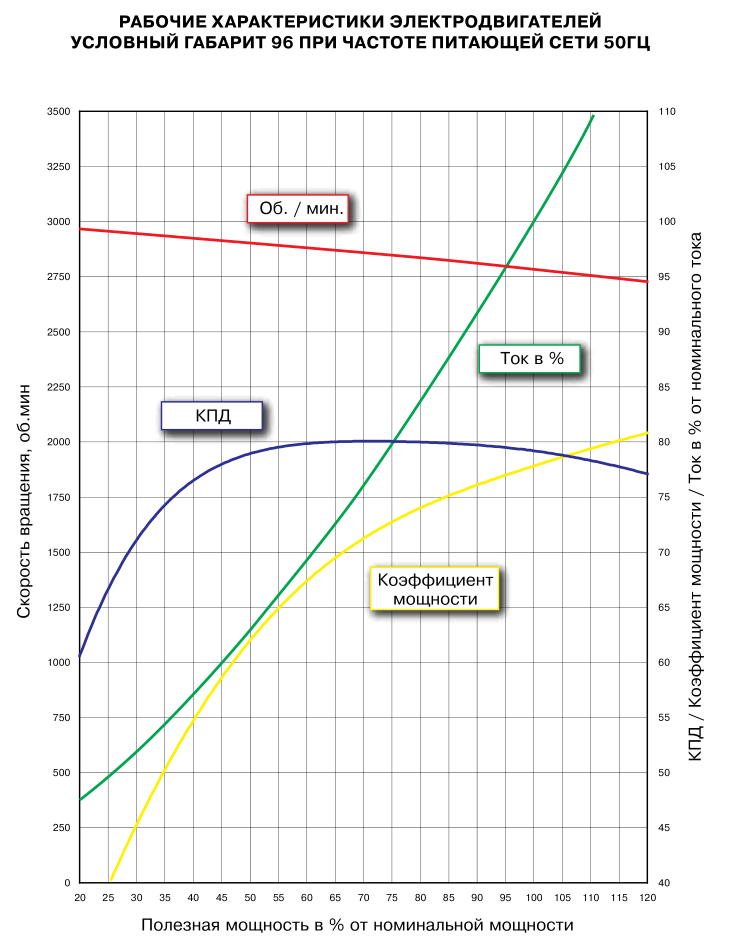
\includegraphics[width=0.6\linewidth]{novomet_motor_1}
	\caption{Каталожные характеристики ПЭД. Источник \cite{Novomet_2013} }
	\label{ris:novomet_motor_1}
\end{figure}

Для асинхронных погружных двигателей производители в каталогах оборудования приводят характеристики, позволяющие оценить КПД, потребляемый ток, частоту вращения вала и коэффициент электрической мощности от загрузки для определенной частоты вращения - рисунок \ref{ris:novomet_motor_1}. Нередко характеристики приводятся для двух частот вращения - 50Гц и 60 Гц.


Каталожная модель погружного АПЭД реализована в расчетных функциях \unf{} как модель двигателя с номером 1  \mintinline{vb.net}{motorID = 1}

Функции для расчета характеристик ПЭД начинаются с префикса \mintinline{vb.net}{motor_}. Описание функций можно найти в приложении "Автоматически сгенерированное описание".



\newpage
\end{comment}       % Глава ЭЦН
%   \section{Моделирование скважины}
Моделирование работы скважины подразумевает расчет распределения давления и температуры в скважине с учетом конструкции скважины и скважинного оборудования. 

Для моделирования скважины требуется задание достаточно большого набора параметров. Попытка уместить эти параметры в функцию, которую можно вызвать из рабочего листа Excel приводит к достаточно сложному поведению функции. Более того от версии к версии поведение может меняться (хотя авторы стараются этого избежать). Поэтому наилучшим способом изучения поведения функций являются эксперименты и изучение кода. Данное описание не претендует на полному. Тем не менее отметим некоторые особенности функций расчета скважины, про которые полезно знать.

\begin{itemize}
	\item Модуль  \mintinline{vb.net}{u7_Excel_functions_well} содержит все функции расчета скважин.
	\item PVT параметры задаются с использованием PVT строки (функция \mintinline{vb.net}{PVT_encode()}). Если PVT строку не задать, расчет проводится для PVT параметров принятых по умолчанию (будут параметры похожие на параметры Приобского месторождения). 
	\item функция умеет учитывать наличие систем механизированной добычи в скважине. Определяется параметром  \mintinline{vb.net}{str_AL}), который должен быть сформирован функциями \mintinline{vb.net}{ESP_encode()}) для ЭЦН или \mintinline{vb.net}{GL_encode()}) для газлифтного метода. Если строку не задать расчёт будет проводиться для фонтанирующей скважины.
	\item  Конструкция скважины может быть задана с использованием числовых параметров глубины скважины, диаметров НКТ и ЭК, либо с использованием массивов (объектов range) содержащих инклинометрию и распределение диаметров по глубине. 
	\item  Модель расчета скважины поддерживает три варианта расчеты температуры - линейную интерполяцию температуры по измеренной глубине, задание температуры окружающей среды от вертикальной глубины и расчет температуры флюида с учетом эмиссии тепла в окружающее пространство где температура задана от вертикальной глубины. Третий вариант расчета самый медленный (требует решения системы двух уравнений на давлений и температуру совместно).
	\item  Модель скважины допускает калибровку с использованием параметров калибровки многофазного потока, параметров калибровки систем мех добычи и калибровки штуцера.
	\item  Все функции с моделями скважин поддерживают вывод расширенного набора параметров с использованием выходных массивов.
\end{itemize}

\subsection{Расчет снизу вверх}
\putlisting{listings/Well_Plin_Pwf_atma.lst}


\subsection{Расчет cверху вниз}
\putlisting{listings/Well_Pwf_Plin_atma.lst}

\section{Расчет узлового анализа}

\putlisting{listings/nodal_pwf_atma.lst}
        % Глава тех режим
%	

\section{Технологический режим добывающих скважин}
Одна из первых реализаций расчётных модулей \unf{} была создана для проведения расчётов потенциала добычи нефти в форме технологического режима добывающих скважин. Расчёты были реализованы в начале 2000х годов. Расчётная форма оказалась удобной для практического применения и со временем алгоритмы расчёта распространились по разным компаниям и широко использовались.

Функции расчета параметров технологического режима добывающих скважин находятся в модуле \mintinline{vb.net}{u_old_mdlTecRegimes}

Для обеспечения обратной совместимости расчётов в \unf{} заложены основные функции расчёта из технологического режима работы скважин. У функций изменены названия функций и имена аргументов, однако алгоритмы расчётов оставлены без изменений.

Пользовательские функции для расчета параметров технологического режима работы добывающих скважин начинаются с префикса  \mintinline{vb.net}{old_}. Листинги определений функций в описании не приводятся, кому интересно, лучше искать непосредственно в коде.

\newpage
\subsection{old\_pwf\_calc\_atma – расчёт забойного давления по динамическому уровню}

Функция рассчитывает забойное давление добывающей нефтяной скважины. Расчёт выполняется по известному значению затрубного давления и динамическому уровню. \cite{Khasanov_TR_2006}

Результат расчёта - абсолютное значение забойного давления. 

Расчёт выполняется по модифицированной корреляции Хасана-Кабира оптимизированной для скорости вычисления как для интервала выше насоса в межтрубном пространстве, так и для участка ниже насоса. При расчёте пренебрегается трением в потоке и используются упрощённые PVT зависимости, что позволило получить результат в аналитическом виде и ускорить расчёты. [ссылку надо будет привести когда то] 

Функция позволяет учесть удлинения скважин для забоя, глубины спуска насоса, и динамического уровня. Два последних значения являются опциональными и могут быть опущены при проведении расчёта. 

%\putlisting{listings/tr_Pwf.txt}



\subsection{old\_pwf\_calc\_p\_intake\_atma – расчёт забойного давления по давлению на приеме}
Функция рассчитывает забойное давление добывающей нефтяной скважины по известному значению давления на приёме насоса. 

Результат расчёта - абсолютное значение забойного давления. 

Расчёт выполняется по модифицированной корреляции Хасана-Кабира оптимизированной для скорости вычисления для участка ниже насоса. При расчёте пренебрегается трением в потоке и используются упрощённые PVT зависимости, что позволило получить результат в аналитическом виде и ускорить расчёты. [ссылку надо будет привести когда то] 

Функция позволяет учесть удлинения скважин для забоя, глубины спуска насоса. Последние значения являются опциональными и могут быть опущены при проведении расчёта. 
%\putlisting{listings/tr_Pwf_calc_Pin_atma.txt}


\subsection{old\_Ppump\_calc\_atma – расчёт давления на приеме по динамическому уровню}
Функция рассчитывает давление на приёме насоса добывающей нефтяной скважины по известному значению затрубного давления и динамическому уровню. 

Расчёт выполняется по модифицированной корреляции Хасана-Кабира оптимизированной для скорости вычисления для участка выше насоса. При расчёте пренебрегается трением в потоке и используются упрощённые PVT зависимости, что позволило получить результат в аналитическом виде и ускорить расчёты. [ссылку надо будет привести когда то]. Значение коэффициента сепарации используется для оценки объёмного расхода газа в межтрубном пространстве. 

Результат расчёта - абсолютное значение давления на приёме насоса. 
%\putlisting{listings/tr_Ppump_calc_atma.txt}



\subsection{old\_Potential\_Pwf\_atma – расчёт целевого забойного давления по доле газа}
Функция рассчитывает целевое забойное давление добывающей нефтяной скважины, при котором достигается заданная доля газа в потоке.

Результат расчёта - абсолютное значение забойного давления. 
%\putlisting{listings/tr_Potential_Pwf_atma.txt}

\subsection{old\_BB\_Pwf\_atma – расчёт забойного давления фонтанирующей скважины по буферному давлению}
Функция рассчитывает забойное давление фонтанирующей добывающей скважины по известному значению буферного давления. Расчет выполняется по корреляции Бегсса Брилла. 

Расчет отличается рядом упрощений - из PVT свойств используется только значение газового фактора - давление насыщения и объемный коэффициент газа вычисляются по корреляциям. 

В отличии от расчёта скважин с насосом в корреляции Беггса Брилла учитывается наличие трения. Хотя для низких дебитов эта корреляция может давать завышенные значения перепада давления. 

Для расчётов рекомендуется использовать функцию \unf{} реализующую аналогичную функциональность с меньшим набором допущений

Результат расчёта - абсолютное значение забойного давления. 
%\putlisting{listings/tr_BB_Pwf_atma.vb}

\subsection{old\_BB\_Pwf\_Pin\_atma – расчёт забойного давления по давлению на приеме по корреляции Беггса-Брилла}
Функция рассчитывает забойное давление  добывающей скважины по известному значению давления на приёме. Расчёт выполняется по корреляции Бегсса-Брилла. 
Расчёт отличается рядом упрощений - из PVT свойств используется только значение газового фактора - давление насыщения и объёмный коэффициент газа вычисляются по корреляциям. 

В отличии от расчёта скважин с насосом в корреляции Беггса Брилла учитывается наличие трения. Хотя для низких дебитов эта корреляция может давать завышенные значения перепада давления. 

Для расчётов рекомендуется использовать функцию \unf{} реализующую аналогичную функциональность с меньшим набором допущений

Результат расчёта - абсолютное значение забойного давления. 

%\putlisting{listings/tr_BB_Pwf_Pin_atma.vb}

        % Глава тех режим
%	\chapter{Упражнения по работе с пользовательскими функциями \unf}

Освоить работу с расчетными функциями \unf{} можно выполняя упражнения описанные в данном разделе и изучая устройство тестовых расчетных модулей. Упражнения демонстрируют некоторые типовые приемы работы с пользовательскими функциями \unf{}. На основе этих приемов можно создать свои расчетные модули решающие специфические задачи пользователя. Примеры не являются исчерпывающими. Варианты работы с расчетными модулями \unf{} не ограничиваются описанными приемами. Цель данного описания - помочь сделать первые шаги в проведении расчетов.
Упражнения помогут: 
\begin{itemize}	
	\item 	освоить принципы работы c пользовательскими функциями \unf{} 
	\item 	изучить основы проведения инженерных расчетов в области добычи нефти
\end{itemize}

\section{Трюки и лайфхаки при работе в excel с функциями \unf{}}
Знание некоторых трюков может сильно упростить работу с пользовательскими функциями \unf{}.
\begin{enumerate}
	\item Для работы с примером должна быть запущена надстройка \unf{}. Убедиться, что надстройка запущена можно найдя вкладку Unifloc в панели меню Excel, рис. \ref{ris:excel_unifloc_tab}.
	
	\begin{figure}[h!]
		\center{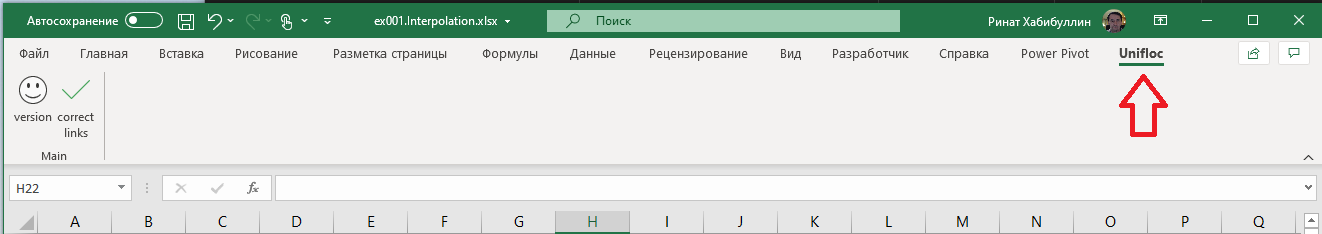
\includegraphics[width=0.8\linewidth]{excel_unifloc_tab}}
		\caption{Открытая панель Unifloc}
		\label{ris:excel_unifloc_tab}
	\end{figure}
	
	\item При необходимости вывести массив значений как результат расчета функций \mintinline{vb.net}{crv_solve} или \mintinline{vb.net}{crv_intersection} используйте комбинацию клавиш \texttt{Cntrl+Shift+Enter} или динамические массивы\footnote{подробнее про динамические массивы (dynamic arrays) можно посмотреть в интернете, например - https://www.planetaexcel.ru/techniques/2/9112/}(для новых версий Excel). Если для динамических массивов требуется подавить вывод массива - используйте знак @ в строке вызова, например как \mintinline{vb.net}{=@crv_solve(...)}.
	
	\item Все названия функций \unf{} начинаются с префикса. Это позволяет быстро искать необходимые функции. При запущенной надстройке достаточно начать вводить в ячейку формулу, например ввести \texttt{=PVT} как Excel откроет выпадающий список с подсказкой, показывающий возможные варианты названий функций (смотри рис. \ref{ris:Ex10_2}). 
	
	\begin{figure}[h!]
		\center{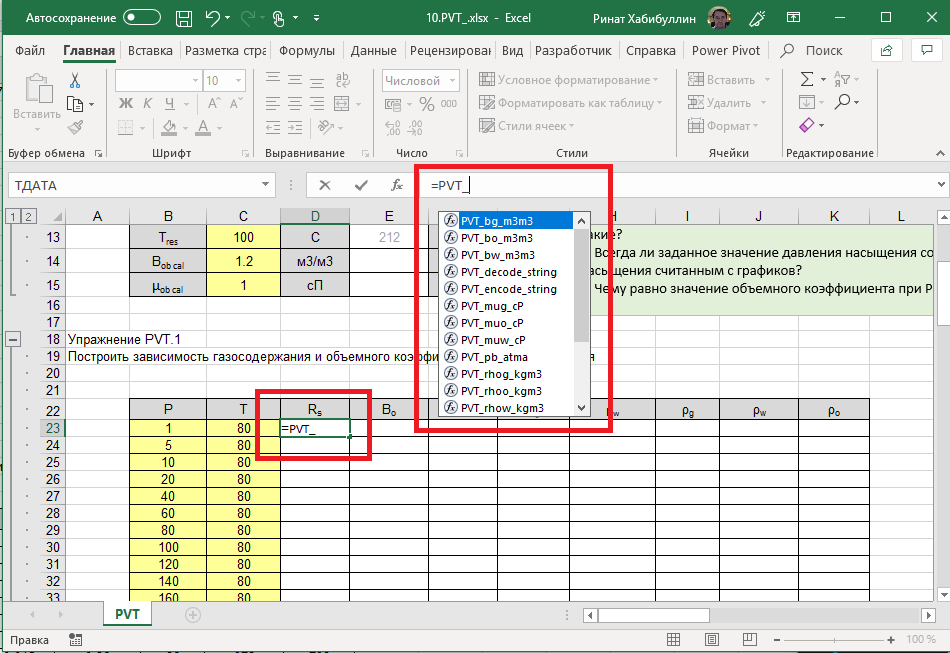
\includegraphics[width=0.8\linewidth]{Ex10_2}}
		\caption{Выпадающий список с подсказками названий функции}
		\label{ris:Ex10_2}
	\end{figure}
	
	\item 	Из выпадающего списка выберите функцию \texttt{=PVT\_Rs\_m3m3(} после чего нажмите кнопку $f_x$ "вставить функцию"  слева от строки формул. Это вызовет окно задания параметров функции, в котором будут указаны все параметры, которые необходимо ввести (смотри рис. \ref{ris:Ex10_3}). В этом окно можно задать необходимые значения параметров или указать ссылки на соответствующие ячейки. Для "хороших" функций в окне задания параметров функции будут подсказки. Также в окне задания параметров можно сразу видеть результат расчета если задан достаточный набор параметров.
	
	\begin{figure}[h!]
		\center{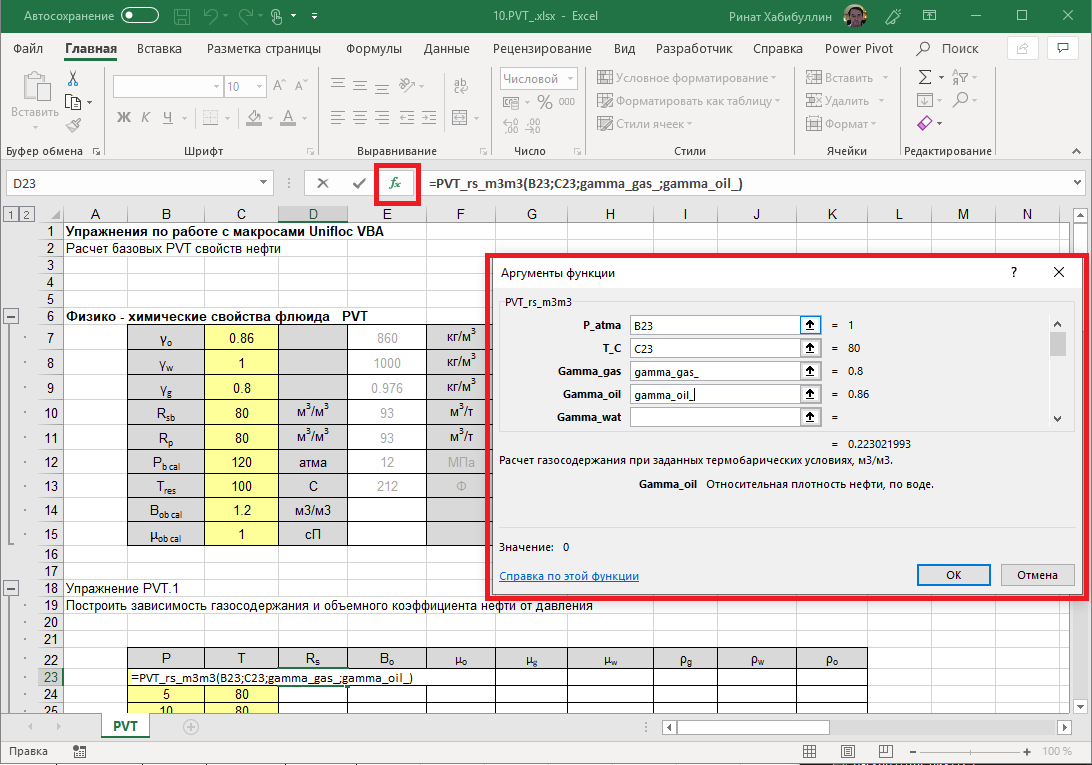
\includegraphics[width=0.8\linewidth]{Ex10_3}}
		\caption{Окно ввода аргументов функции}
		\label{ris:Ex10_3}
	\end{figure}
	
	\item После ввода всех параметров и нажатия кнопки ОК в ячейке должен отобразиться результат расчета. Воспользовавшись инструментом "Влияющие ячейки" на вкладке "Формулы"\ можно отследить на какие ячейки ссылается введенная формула (смотри рис. \ref{ris:Ex10_4})
	\begin{figure}[h!]
		\center{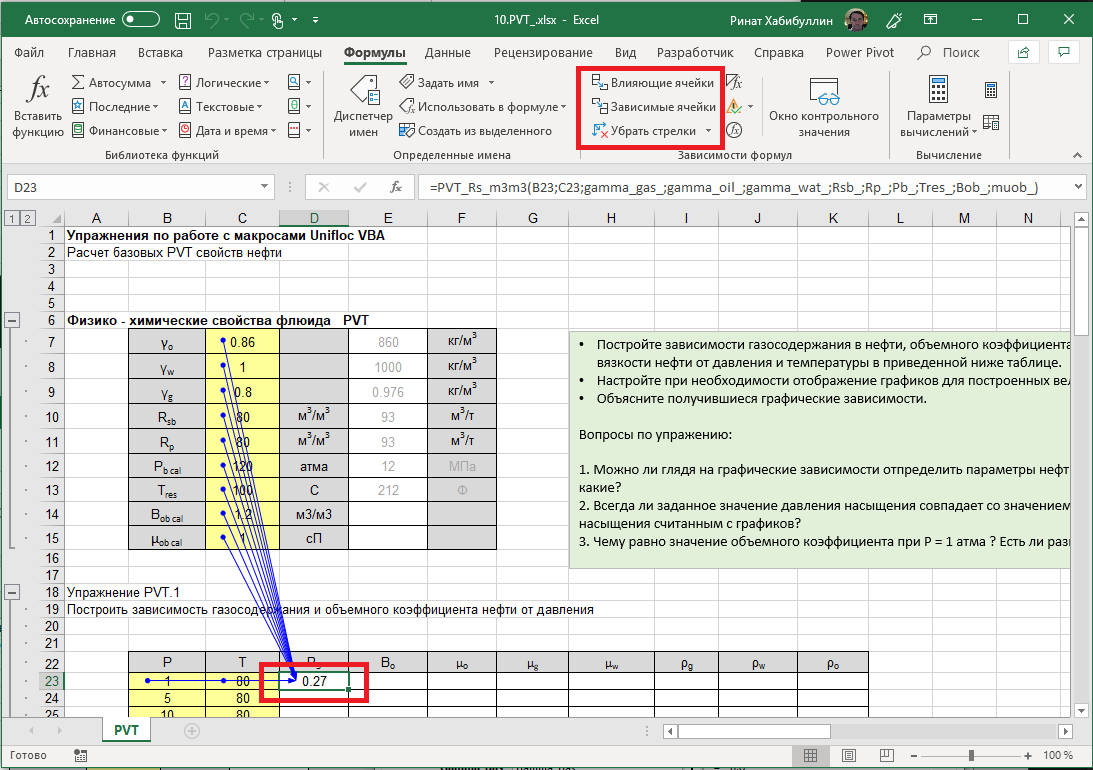
\includegraphics[width=0.8\linewidth]{Ex10_4}}
		\caption{Результат вызова пользовательской функции с отображение влияющих ячеек}
		\label{ris:Ex10_4}
	\end{figure}
\end{enumerate}


\section{Работа с таблично заданными кривыми}
Инженерный анализ требует умения ловко работать с графическими данными - кривыми, картами, кросс плотами и графиками. Кроме отображения графических данных, что легко делается стандартными программами - часто требует проводить по ним расчеты. Набор функций \unf{} для работы с таблично заданными кривыми может оказать полезными для этих целей. 

Функции \unf{} для работы с таблично заданными кривыми начинаются с префикса \mintinline{vb.net}{crv_}, от слова curve. Доступна функциональность
\begin{itemize}	
	\item интерполяции различными методами (работает и экстраполяция)
	\item поиска решения уравнения вида $f(x) = с$ где функция $f(x)$ задана таблицей (ищется решение для линейной аппроксимации)
	\item поиска пересечений двух кривых заданных таблицами (ищется решение для линейно аппроксимации)	
\end{itemize}
В коде можно обнаружить еще ряд функций, но они не будут описываться в данном руководстве, хотя по ним можно найти примеры в папке \texttt{examples} репозитория.

\subsection{ \texttt{ex001.Interpolation.xlsx} - Интерполяция табличных кривых}
Файл примера \texttt{ex001.Interpolation.xlsx} можно найти в папке \texttt{exercises} репозитория \unf{}.

\begin{enumerate}
	\item Для работы с примером должна быть запущена надстройка \unf{}. Убедиться, что надстройка запущена можно найдя вкладку Unifloc в панели меню Excel, рис. \ref{ris:excel_unifloc_tab}.
	

	
	\item Откройте файл с упражнением \texttt{ex001.Interpolation.xlsx} (смотри рис. \ref{ris:Ex001_1}).
	
	\begin{figure}[h!]
		\center{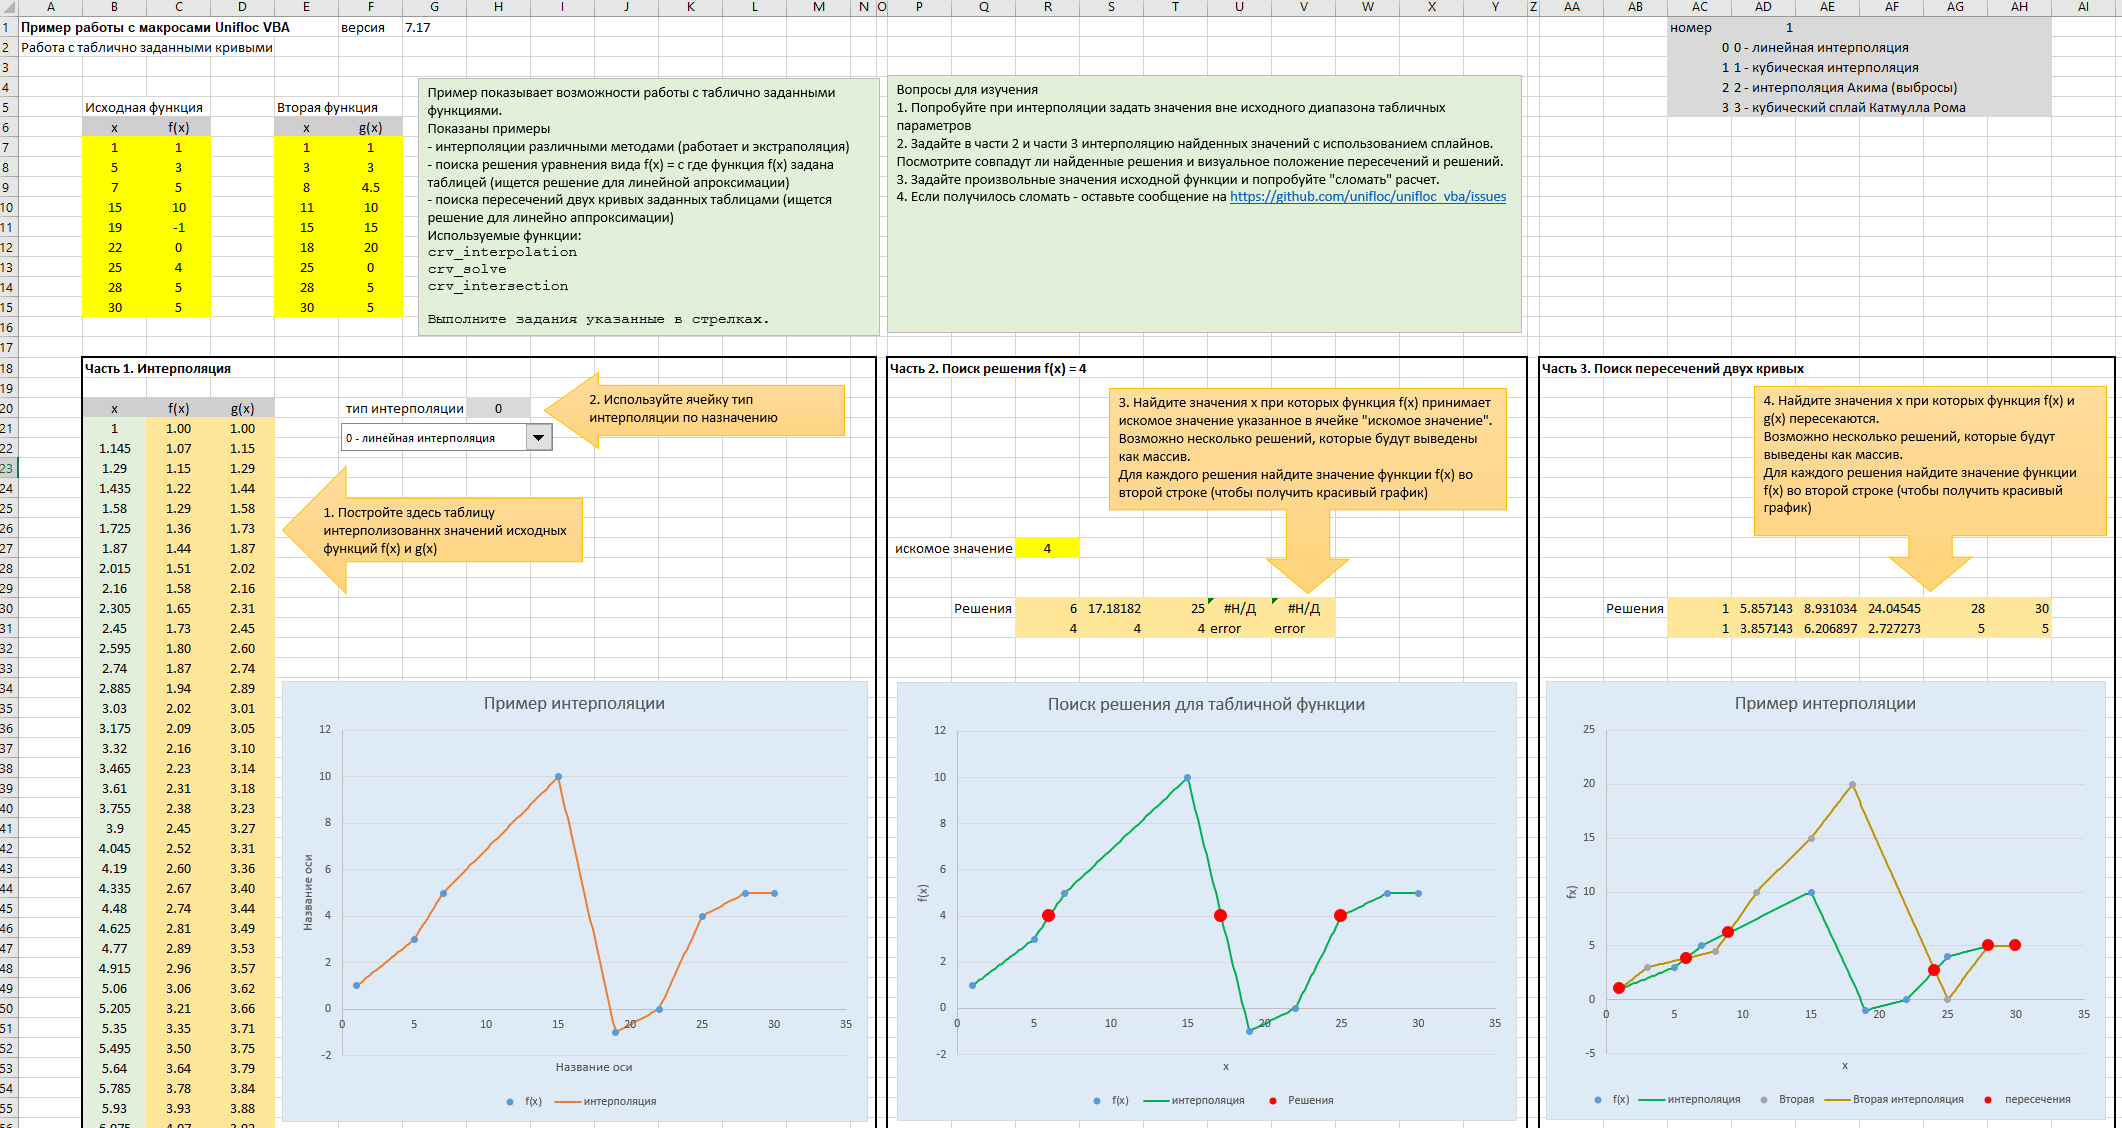
\includegraphics[width=1\linewidth]{Ex001_1}}
		\caption{Упражнение \texttt{ex001.Interpolation.xlsx} со всеми заполненными полями}
		\label{ris:Ex001_1}
	\end{figure}
	
	Пример разделен на три части: Часть 1. Интерполяция; Часть 2. Поиска решения $f(x)=c$; Часть 3.Поиск пересечения двух кривых.
	
	\item Выполните задания указанные в стрелках (последовательность выполнения по номерам стрелок). При этом должны автоматически построиться графики как на рисунке \ref{ris:Ex001_1}).
	
	\item Постарайтесь ответить на вопросы в блоке "Вопросы для изучения"

\end{enumerate}

\section{ \texttt{ex010.PVT.xlsm} - Расчет базовых PVT свойств флюидов}

Расчет физико химических свойств пластовых флюидов (PVT параметров) лежит в основе всех расчетов систем нефтедобычи. При решении прикладных задач редко возникает необходимость расчета PVT свойств непосредственно, однако понимание принципа их расчета, а особенно зависимости результатов расчета от исходных данных важно.
   
Для выполнения упражнения используйте файл \texttt{ex010.PVT.xlsm} (смотри рис. \ref{ris:Ex10_1}).

\begin{figure}[h!]
	\center{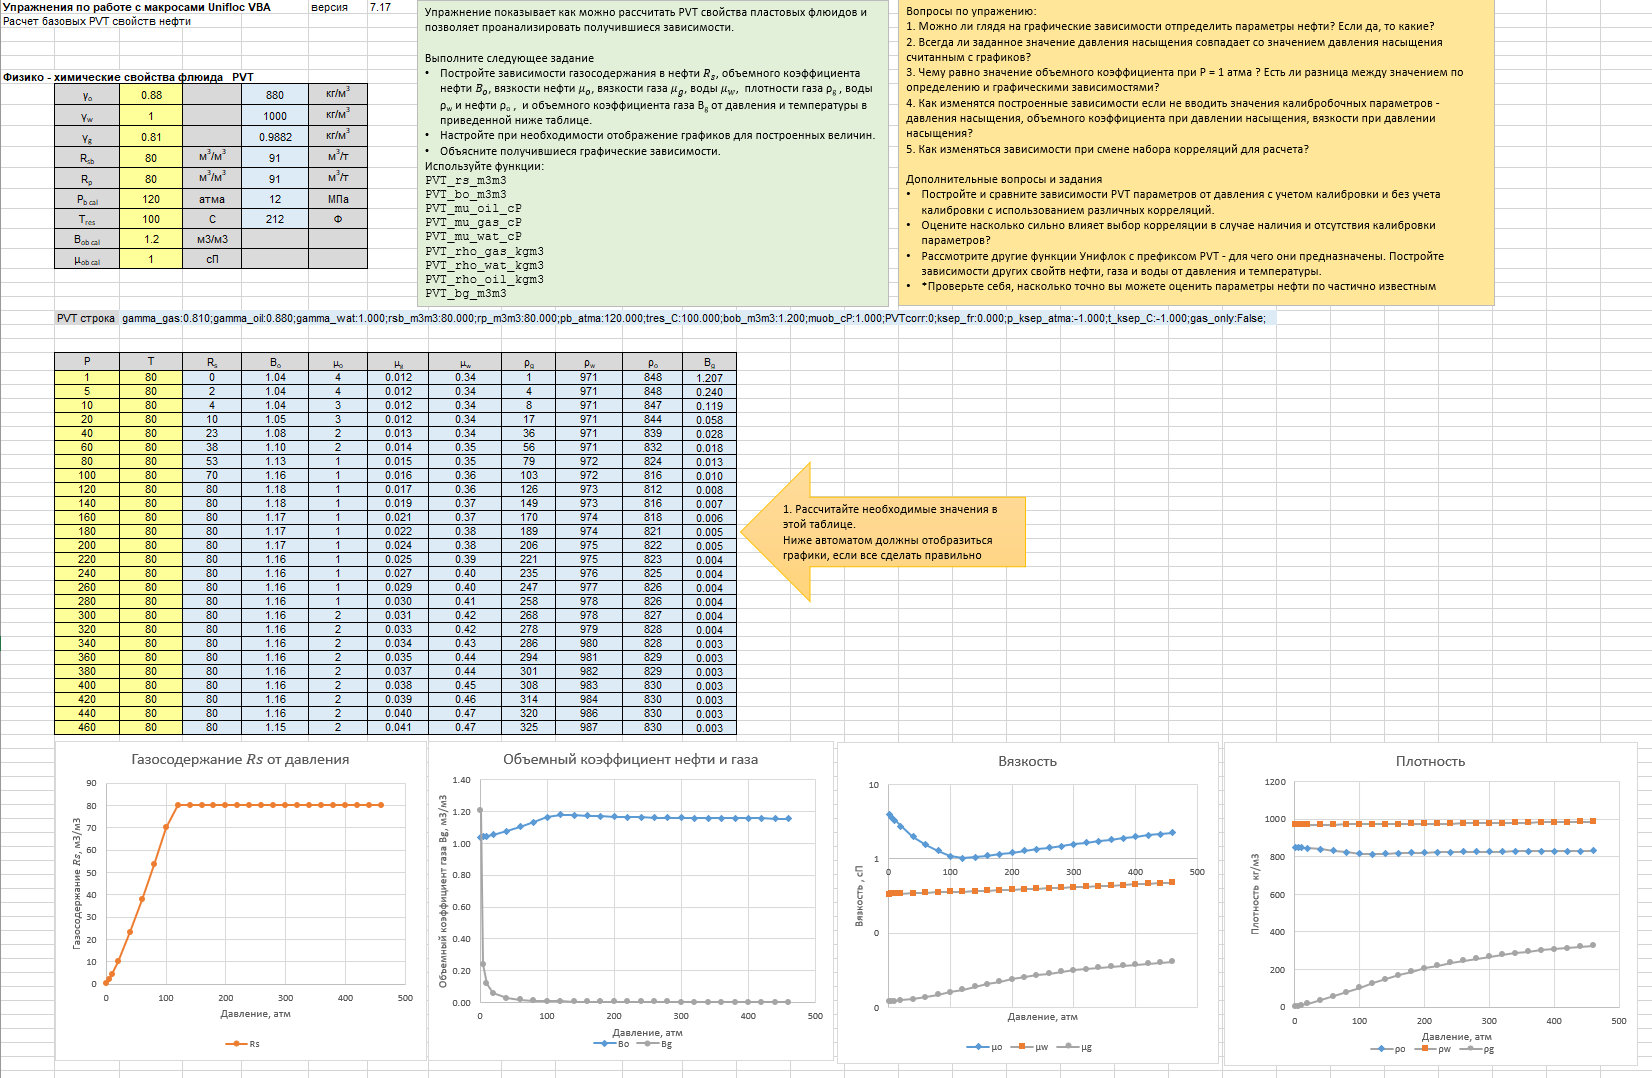
\includegraphics[width=1\linewidth]{Ex10_1}}
	\caption{Упражнение \texttt{ex010.PVT.xlsx} со всеми заполненными полями.}
	\label{ris:Ex10_1}
\end{figure}

\subsection{Упражнение}
Упражнение показывает как рассчитать PVT свойства пластовых флюидов и позволяет проанализировать получившиеся зависимости. 

Выполните следующие задания
\begin{enumerate}
	\item  Постройте зависимости газосодержания в нефти $R_s(P,T)$, объемного коэффициента нефти $B_o(P,T)$, вязкости нефти $\mu_o(P,T)$, вязкости газа $\mu_g(P,T)$, воды $\mu_w(P,T)$,  плотности газа $\rho_g(P,T)$ , воды $\rho_w(P,T)$ и нефти $\rho_o(P,T)$ ,  и других PVT параметров от давления и температуры. 
	
	\item  Убедитесь, что для всех построенных графиков вы понимаете их поведение при изменении давления и температуры. 
	
\end{enumerate}

Для выполнения расчетов используйте функции \unf{} начинающиеся с префикса \texttt{PVT\_}:




\subsection{Вопросы для самоконтроля}
Для самоконтроля ответьте на следующие вопросы:

\begin{enumerate}
	
	\item Можно ли глядя на графические зависимости определить параметры нефти? Если да, то какие?
	
	\item Всегда ли заданное значение давления насыщения совпадает со значением считанным с графиков?
	
	\item Чему равно значение объемного коэффициента $B_o$ при $P = 1$ атма? Есть ли разница между значением по определению и графическими зависимостями? Если разница есть, то каким параметром она может быть вызвана? Постройте график иллюстрирующий данную зависимость.
	
	\item Чему равно значение газосодержания $r_s$ при $P = 1$ атма? Есть ли разница между значением по определению и графическими зависимостями? Если разница есть, то каким параметром она может быть вызвана? Постройте график иллюстрирующий данную зависимость.
	
 	\item Как изменятся построенные зависимости если не вводить значения калибровочных параметров - давления насыщения, объемного коэффициента при давлении насыщения, вязкости при давлении насыщения?
	
	\item 	Как изменяться зависимости PVT параметров от давления и температуры при смене набора корреляций для расчета?
	
\end{enumerate}

\subsection{Дополнительные вопросы и задания}

	Для того, чтобы глубже разобраться в расчете свойств флюидов с использованием \unf{} ответьте на дополнительные вопросы, которые легко превращаются в задания.

\begin{enumerate}
	
	\item Постройте и сравните зависимости PVT параметров от давления с учетом калибровки и без учета калибровки с использованием различных корреляций. Что важнее - правильно выбрать корреляцию или задать корректные калибровочные параметры?
	
	\item Оцените насколько сильно влияет выбор корреляции в случае наличия и отсутствия калибровки параметров?
	
	\item Рассмотрите другие функции Унифлок с префиксом PVT - для чего они предназначены. Постройте зависимости других свойтв нефти, газа и воды от давления и температуры. 
	
	\item *Проверьте себя, насколько точно вы можете оценить параметры нефти по частично известным данным? Какой минимальный набор данных надо знать? Проверьте коллег попросив их оценить/угадать свойства нефти по частичным данным. 
	
	\item Простой пример - часто нет данных по плотности газа (например в технологическом режиме добывающих скважин). Можно ли восстановить этот параметр по другим данным?
	
	\item Можно ли оценить величину газосодержания нефти по плотности нефти и газа?
	
	\item Можно ли оценить плотность нефти по газосодержанию и давлению насыщения?
	
\end{enumerate}


\section{\texttt{ex011.MF\_gas\_fraction.xlsm} - Расчет свойств потока флюидов}

PVT функции описывают свойства флюидов. Можно представить себе, что они описывают свойства флюидов находящихся в PVT бомбе - устройстве для отбора проб. В этом случае флюиды неподвижны и находятся в равновесном состоянии. На практике приходится иметь дело с флюидами двигающимися в скважине или трубопроводе - с потоком флюидов. В потоке флюидов добавляются дополнительные параметры -- расход флюидов или дебит $Q_{liq}, Q_g$ и обводненность $f_w$ -- показатель показывающий объемную долю воды в потоке. 
Функции работающие с потоками в \unf{} имеют префикс \mintinline{vb.net}{MF_}. Префикс должен намекать на многофазность потока и на самом деле плох с лингвистической точки зрения (multiphase - has no F letter), но удобен с программистской точки зрения и уже поздно его менять.

Файл примера \texttt{ex011.MF\_gas\_fraction.xlsm} можно найти в папке \texttt{exercises} репозитория \unf{} (смотри рис. \ref{ris:Ex11_1}).

\begin{figure}[h!]
	\center{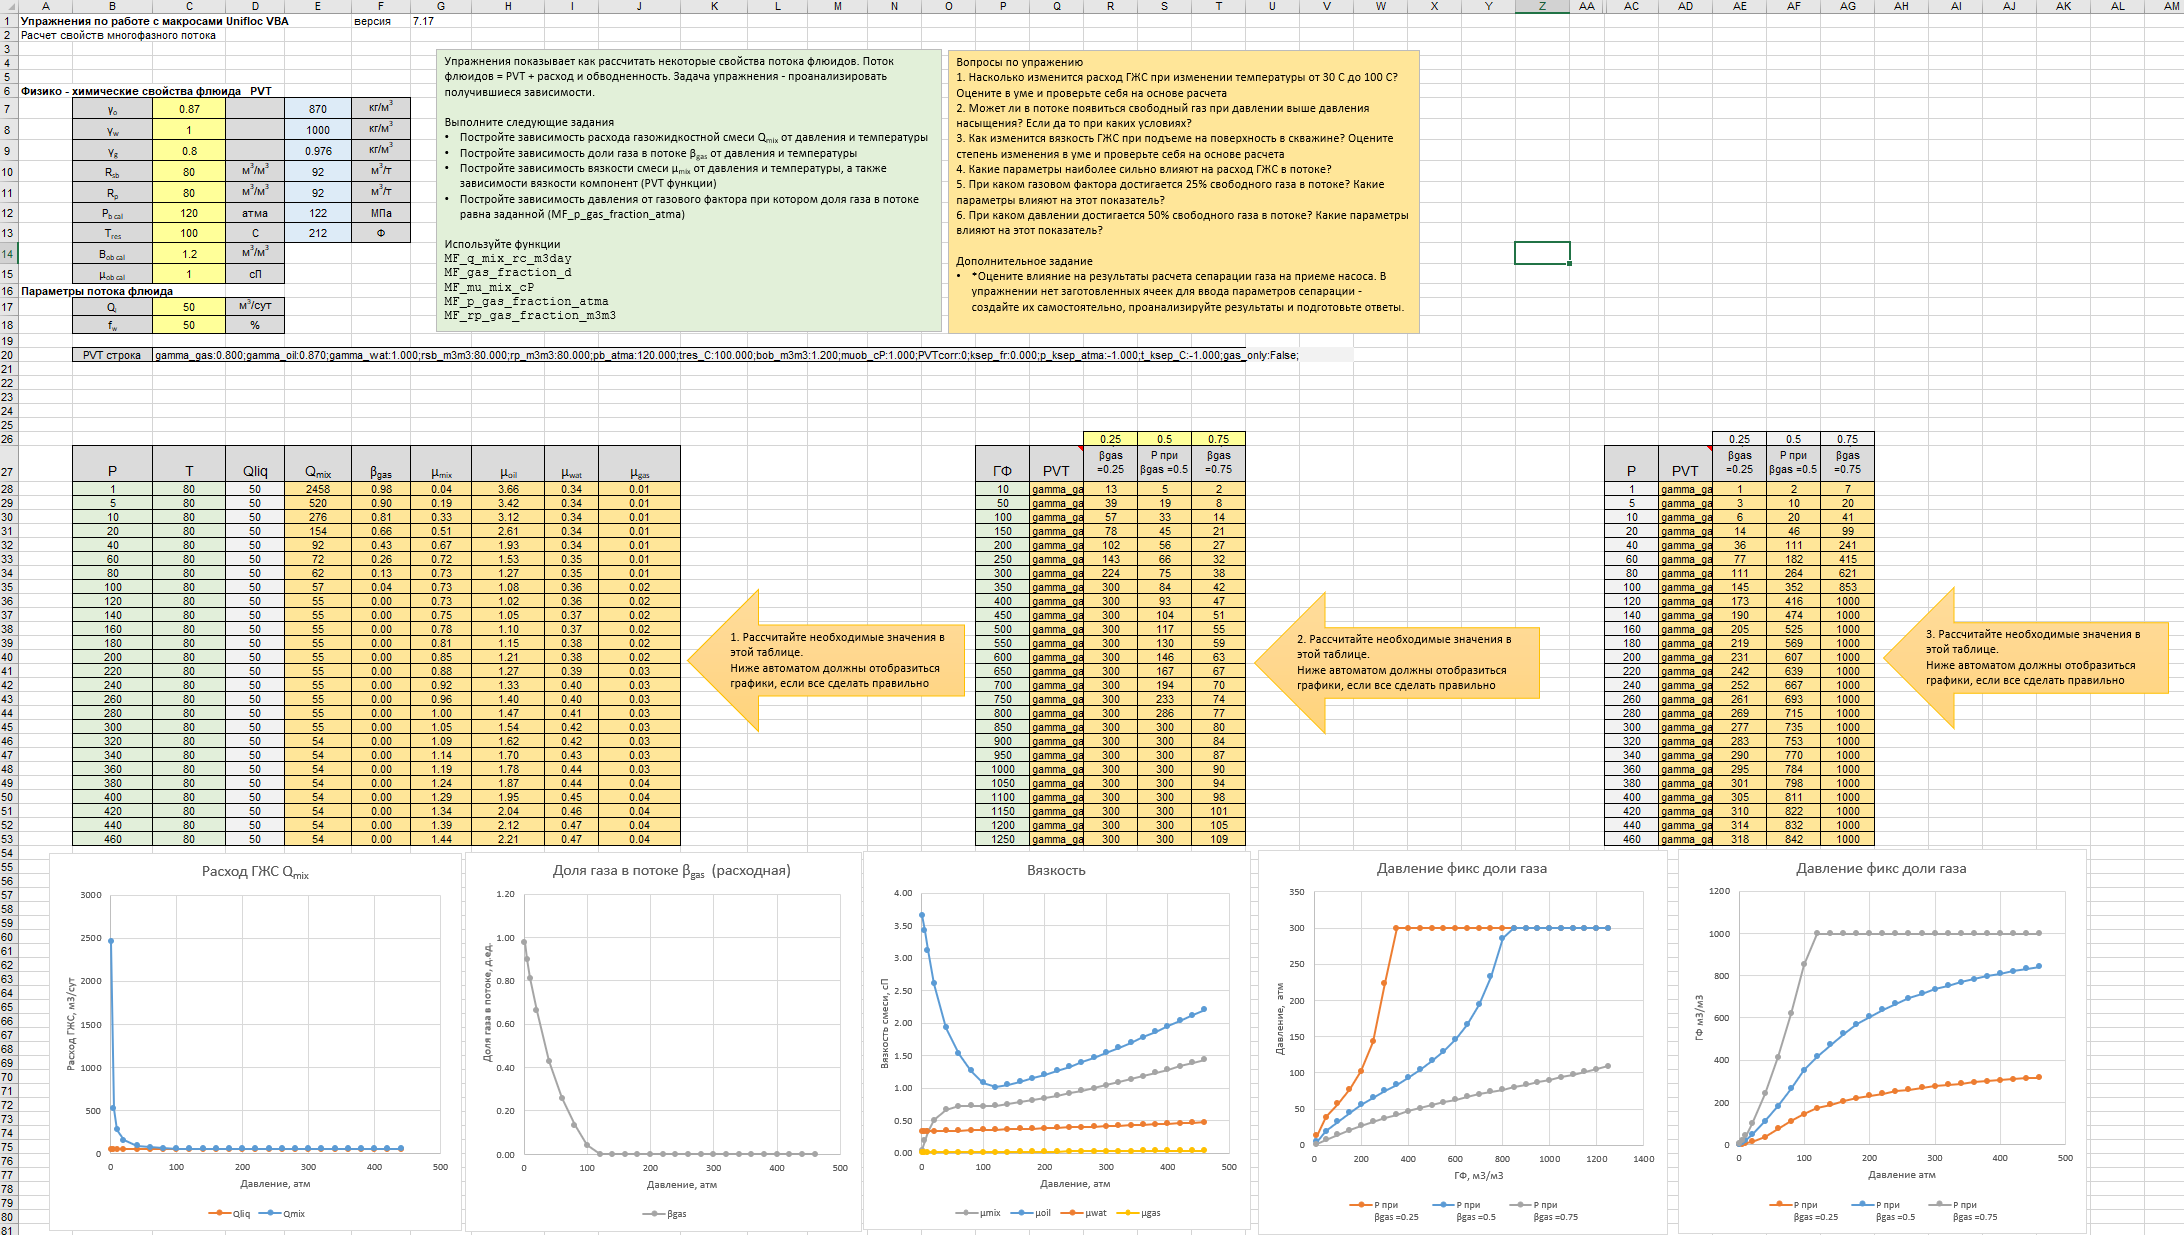
\includegraphics[width=1\linewidth]{Ex11_1}}
	\caption{Упражнение \texttt{ex011.MF\_gas\_fraction.xlsm}  со всеми заполненными полями }
	\label{ris:Ex11_1}
\end{figure}

\subsection{Упражнение}
Упражнение показывает как рассчитать некоторые свойства потока флюидов. Поток флюидов = PVT + расход и обводненность. Задача упражнения - проанализировать получившиеся зависимости.

Выполните следующие задания
\begin{enumerate}
	\item Постройте зависимость расхода газожидкостной смеси $Q_{mix}(P,T)$ от давления $P$ и температуры $T$; 
	\item Постройте зависимость доли газа в потоке $\beta_{gas}(P,T)$ от давления $P$ и температуры $T$;
	\item Постройте зависимость вязкости смеси $\mu_{mix}(P,T)$ от давления $P$ и температуры $T$, а также зависимости вязкости отдельных компонент от давления $P$ и температуры $T$; 
	\item Постройте зависимость давления  от газового фактора $P(R_p)$ при котором доля газа в потоке  равна заданной  $P(R_p)|_{\beta_{gas} = const}$;
	
	\item Постройте зависимость газового фактора от давления $R_p(P)$  при котором доля газа в потоке равна заданной $R_p(P)|_{\beta_{gas} = const}$; 
 	
\end{enumerate}

Для выполнения расчетов используйте следующие функции \unf{}:
\begin{itemize}

	\item \texttt{MF\_q\_mix\_rc\_m3day}
	\item \texttt{MF\_gas\_fraction\_d}
	\item \texttt{MF\_mu\_mix\_cP}
	\item \texttt{MF\_p\_gas\_fraction\_atma}
	\item \texttt{MF\_rp\_gas\_fraction\_m3m3}

\end{itemize}

Убедитесь, что для всех построенных графиков вы понимаете их поведение при изменении давления и температуры. 

\subsection{Вопросы для самоконтроля}
Для самоконтроля ответьте на следующие вопросы:

\begin{enumerate}
	
	\item Насколько изменится расход ГЖС при изменении температуры от 30 \textdegree С до 100 \textdegree С? Оцените ответ в уме и проверьте себя на основе расчета. Что еще надо учесть кроме температуры?
	
	\item Может ли в потоке появиться свободный газ при давлении выше давления насыщения? Если да то при каких условиях?
	
	\item Как изменится вязкость ГЖС при подъеме на поверхность в скважине? Оцените степень изменения в уме и проверьте себя на основе расчета.
	
	\item Какие параметры наиболее сильно влияют на расход ГЖС в потоке?
	
	\item При каком газовом факторе достигается 25\% свободного газа в потоке? Какие параметры влияют на этот показатель?
	 	
	\item При каком давлении достигается 50\% свободного газа в потоке? Какие параметры влияют на этот показатель?
	 	
\end{enumerate}

\subsection{Дополнительные вопросы и задания}

Для того, чтобы глубже разобраться в расчете свойств флюидов с использованием \unf{} ответьте на дополнительные вопросы, которые легко превращаются в задания.

\begin{enumerate}
	
	\item *Оцените влияние на результаты расчета сепарации газа на приеме насоса. В упражнении нет заготовленных ячеек для ввода параметров сепарации - создайте их самостоятельно, проанализируйте результаты и подготовьте ответы.
	
	
	
\end{enumerate}


В дополнительном задании говорится о сепарации газа на приеме насоса. Имеется в виду следующее - если у нас есть пластовые флюиды, свойства которых мы знаем и можем задать, то после сепарации части свободного газа, что часто происходит на скважинном насосе, свойства флюида изменятся. Изменится его эффективное давление насыщения (потому что мы убрали часть газа) и газосодержание при давлении насыщения. И соответственно поплывут и остальные свойства. Это можно учесть задав в \mintinline{vb.net}{PVT_Encode()} три параметра - коэффициент сепарации газа $K_{sep}$, давление при которой произошла сепарации $P_{sep}$ и температуру при которой произошла сепарация $T_{sep}$. Подробнее про это можно найти в соответствующих разделах (поэтому тут это задание дополнительное).

\section{\texttt{ex012.PVT\_z\_factor.xlsm} - Пример расчета свойств газа}

Как рассчитать коэффициент сверхсжимаемости газа и какие могут быть неожиданности. 

\section{\texttt{ex013.PVT\_hydrates.xlsm} - Расчет кривой образования гидратов}

Пример показывает, как можно оценить кривые образования гидратов
 % Глава описание упражнений про PVT

\section{\texttt{ex020.IPR.xlsm} - Расчет производительности скважины}

Стационарная модель притока к скважине (закон Дарси с поправкой Вогеля) - одна из самых простых и распространенных моделей, широко применяемая в индустрии. \unf{} содержит функции позволяющие упростить расчет индикаторной кривой. Такие функции имеют префикс \mintinline{vb.net}{IPR_} от Inflow Performance Relationship.

Файл примера \mintinline{vb.net}{ex020.IPR.xlsm} можно найти в папке \texttt{exercises} репозитория \unf{} (смотри рис. \ref{ris:Ex20_1}).

\begin{figure}[h!]
	\center{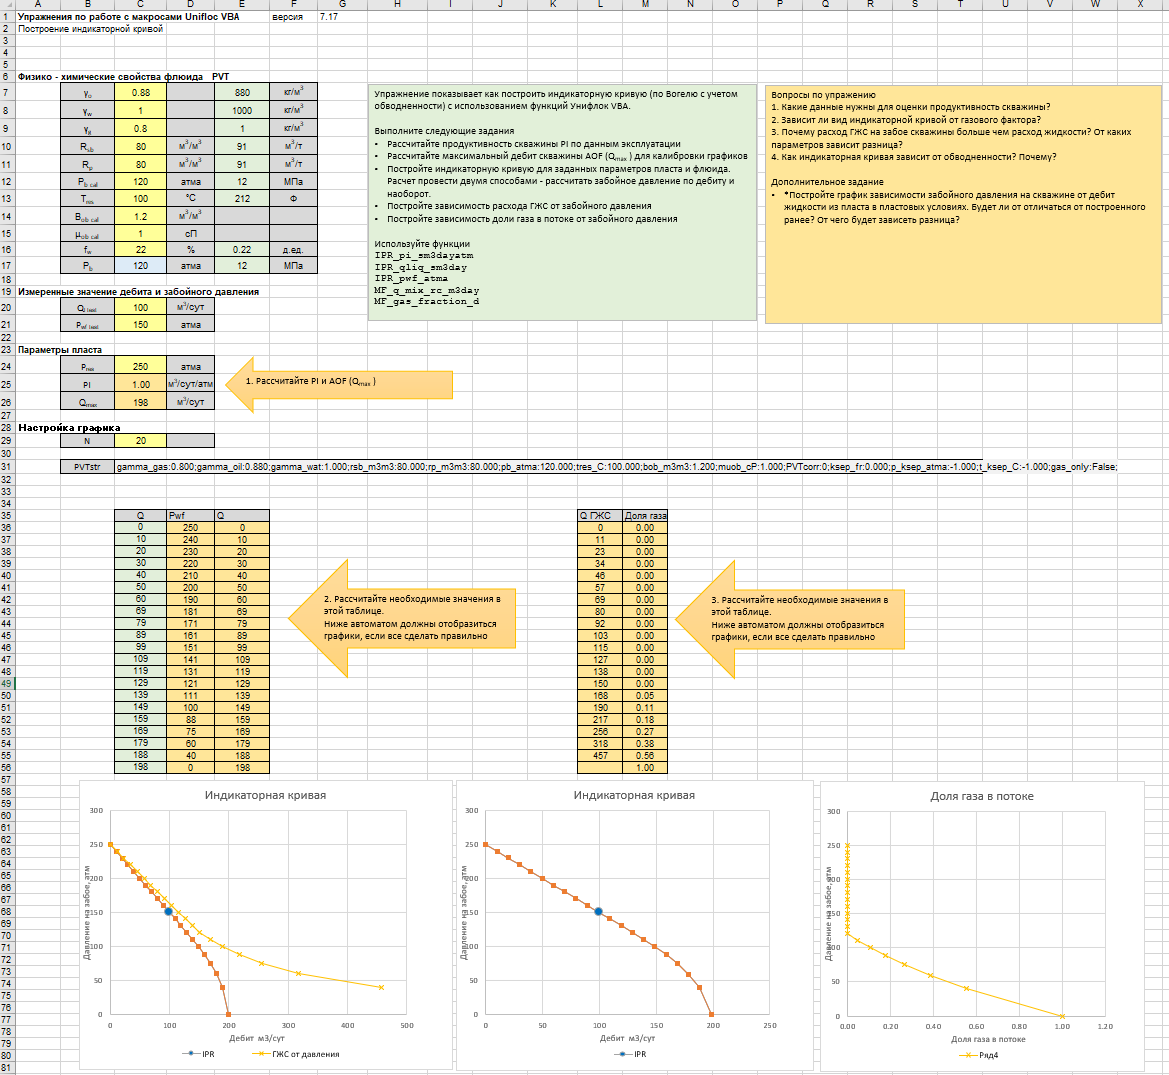
\includegraphics[width=1\linewidth]{Ex20_1}}
	\caption{Упражнение \mintinline{vb.net}{ex020.IPR.xlsx} со всеми заполненными полями }
	\label{ris:Ex20_1}
\end{figure}


\subsection{Упражнение}
Упражнение показывает как построить индикаторную кривую (по Вогелю с учетом обводненности) с использованием функций \unf{}.
 

Выполните следующие задания
\begin{enumerate}
	\item  Рассчитайте продуктивность скважины PI по данным эксплуатации
	\item  Рассчитайте максимальный дебит скважины $AOF=Q_{max}|_{P_{wf}=1}$ для калибровки графиков
	 	 
	\item  Постройте индикаторную кривую для заданных параметров пласта и флюида. Расчет проведите двумя способами - рассчитайте забойное давление по дебиту и наоборот.
	\item  Постройте зависимость расхода ГЖС от забойного давления 
	\item  Постройте зависимость доли газа в потоке от забойного давления
\end{enumerate}


Для выполнения расчетов используйте следующие функции \unf{}:
\begin{itemize}
	
	\item \texttt{IPR\_pi\_sm3dayatm	}
	\item \texttt{IPR\_qliq\_sm3day}
	\item \texttt{IPR\_pwf\_atma}
	\item \texttt{MF\_q\_mix\_rc\_m3day}
	\item \texttt{MF\_gas\_fraction\_d}
	
\end{itemize}


Коэффициент продуктивности $PI$ скважины рассчитывается в ячейке С25 по замеренным данным  с помощью функции

{ \small  \texttt{=IPR\_PI\_sm3dayatm(qltest\_;Pwftest\_;Pres\_;fw\_;Pb\_)}}

А максимальный дебит $Q_{max}$ при максимальной депрессии с забойным давлением равным нулю

{ \small  \texttt{=IPR\_Qliq\_sm3Day(PI\_;Pres\_;0;fw\_;Pb\_)}}


\subsection{Вопросы для самоконтроля}
Для самоконтроля ответьте на следующие вопросы:

\begin{enumerate}
	
	\item Какие данные нужны для оценки продуктивности скважины? Есть два варианта ответа - чем они отличаются между собой?
	
	\item Зависит ли вид индикаторной кривой от газового фактора?
	
	\item Почему расход ГЖС на забое скважины больше чем расход жидкости? От каких параметров зависит разница?
	
  	\item Как индикаторная кривая зависит от обводненности? Почему?
	
	
\end{enumerate}

\subsection{Дополнительные вопросы и задания}

Для того, чтобы глубже разобраться в расчете притока из пласта с использованием \unf{} ответьте на дополнительные вопросы, которые легко превращаются в задания.

\begin{enumerate}
	
	\item  *Постройте график зависимости забойного давления на скважине от дебита жидкости из пласта в пластовых условиях. Будет ли от отличаться от построенного ранее? От чего будет зависеть разница?
	
	
\end{enumerate} % Глава описание упражнений про IPR

\section{\texttt{ex040.MF\_choke.xlsm} - Расчет штуцера}

Для контроля дебита и/или давления на добывающих скважинах вблизи устья может устанавливаться штуцер. Для штуцера, как для любого гидравлического элемента, возможно 4 варианта расчета - расчет давления по потоку, расчет давления против потока, расчет потока по давлениям и настройка модели штуцера по известным давлениям и потоку. В упражнении демонстрируются все варианты расчета. 

Файл примера \mintinline{vb.net}{ex040.MF_choke.xlsx} можно найти в папке \texttt{exercises} репозитория \unf{}.

\begin{figure}[h!]
	\center{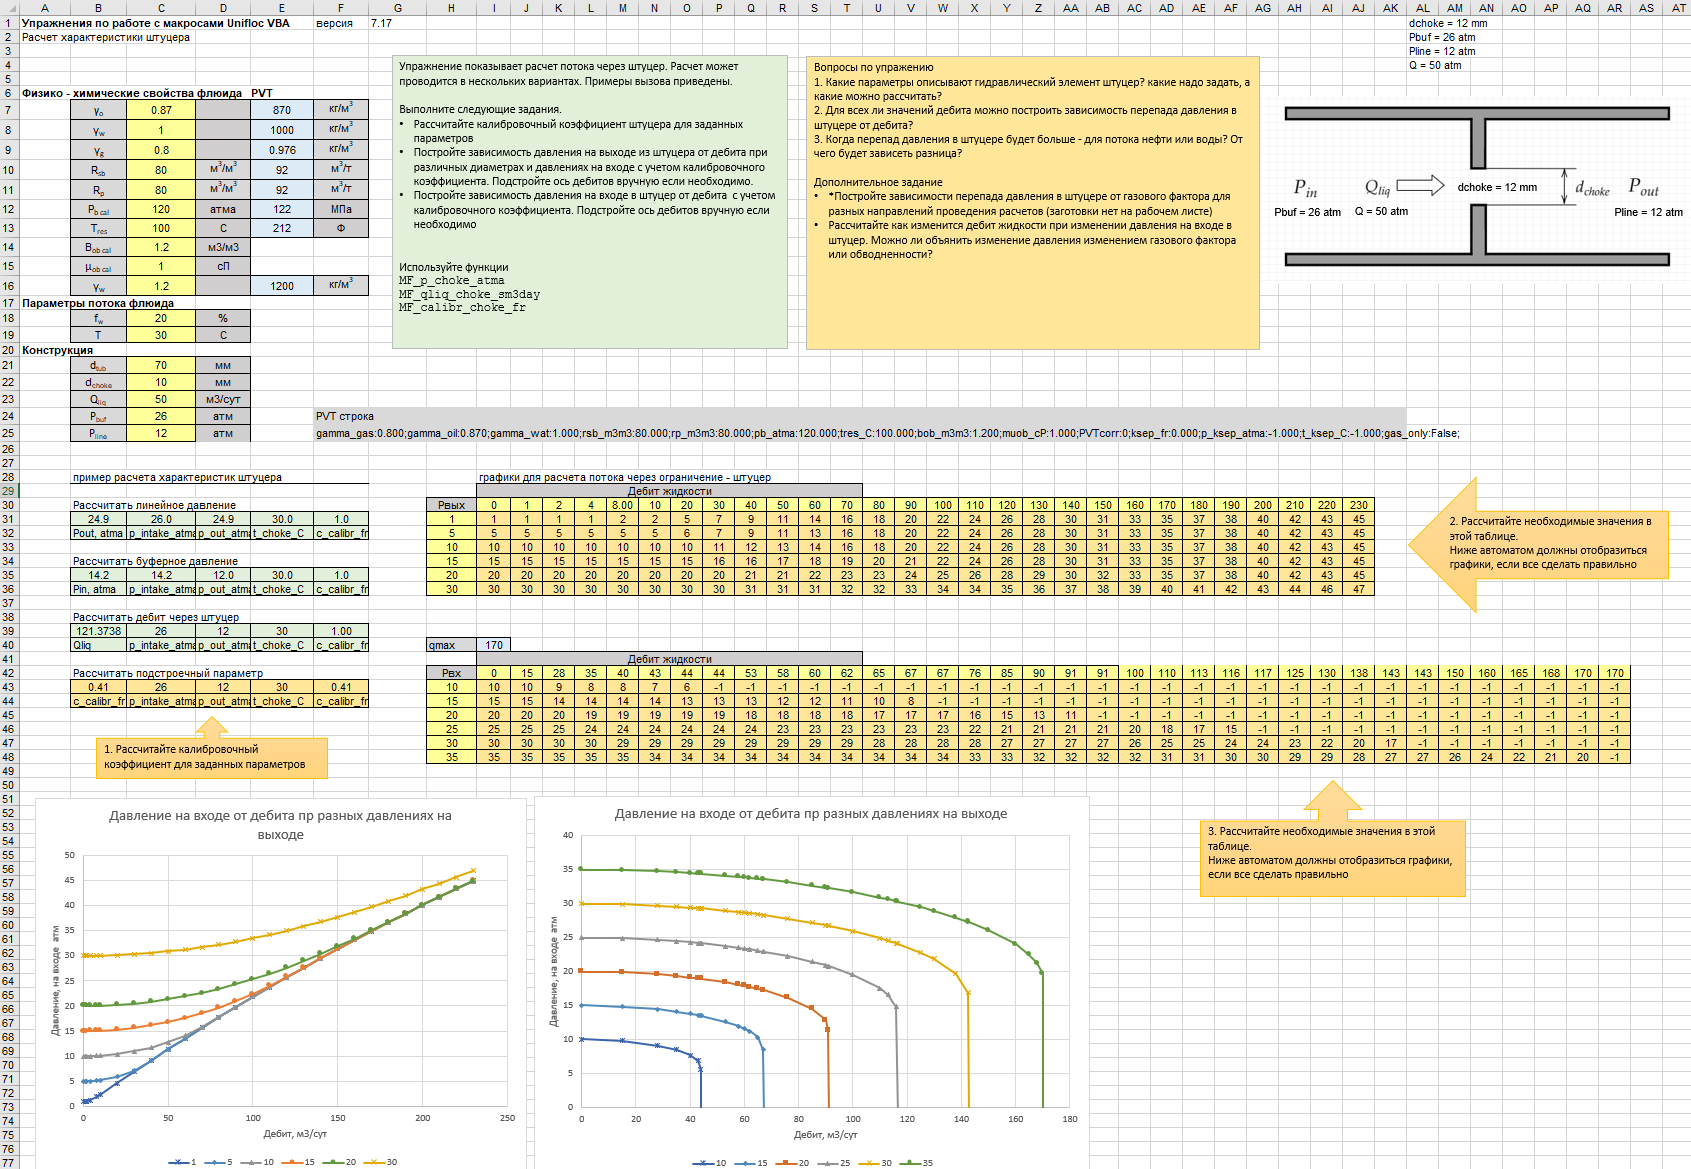
\includegraphics[width=1\linewidth]{Ex40_1}}
	\caption{Упражнение \mintinline{vb.net}{ex040.MF_choke.xlsx} со всеми заполненными полями }
	\label{ris:Ex40_1}
\end{figure}


\subsection{Упражнение}
Выполните следующие задания.
\begin{enumerate}
	\item Рассчитайте калибровочный коэффициент штуцера для заданных параметров
	\item Постройте зависимость давления на выходе из штуцера от дебита при различных диаметрах и давлениях на входе с учетом калибровочного коэффициента. Подстройте ось дебитов вручную если необходимо.
	\item Постройте зависимость давления на входе в штуцер от дебита  с учетом калибровочного коэффициента. Подстройте ось дебитов вручную если необходимо 
\end{enumerate}

Для выполнения расчетов используйте следующие функции \unf{}:
\begin{itemize}
	
	\item \mintinline{vb.net}{MF_p_choke_atma}
	\item \mintinline{vb.net}{MF_qliq_choke_sm3day}
	\item \mintinline{vb.net}{MF_calibr_choke_fr}
	
\end{itemize}

\subsection{Вопросы для самоконтроля}
Для самоконтроля ответьте на следующие вопросы:

\begin{enumerate}
	
	\item Какие параметры описывают гидравлический элемент штуцер? Какие надо задать, а какие можно рассчитать?
	\item Для всех ли значений дебита можно построить зависимость перепада давления в штуцере от дебита?
	\item Когда перепад давления в штуцере будет больше - для потока нефти или воды? От чего будет зависеть разница?
	\item Изменением каких параметров можно откалибровать расчет для штуцера? На что они влияют?
	
\end{enumerate}

\subsection{Дополнительные вопросы и задания}

Для того, чтобы глубже разобраться в расчете потока через штуцер с использованием \unf{} ответьте на дополнительные вопросы, которые легко превращаются в задания.

\begin{enumerate}
	
	\item  Постройте зависимости перепада давления в штуцере от газового фактора для разных направлений проведения расчетов. Чем зависимость будет отличаться от аналогичной для дебита жидкости? 
	\item Рассчитайте как изменится дебит жидкости при изменении давления на входе в штуцер. Можно ли объяснить изменение давления изменением газового фактора или обводненности?
	\item Рассчитайте работу штуцера для потока газа.  Как изменится перепад давления для газа по сравнению с ГЖС?
	
\end{enumerate}

Установите \mintinline{vb.net}{gas_only=True} для PVT строки для проведения расчета для газа. Расход газа при этом задается параметром \mintinline{vb.net}{q_gas_sm3day} в функциях расчета штуцера. % Глава описание упражнений про штуцер

\section{\mintinline{vb.net}{ex051.MF_pipeline.xlsm} - Расчет распределения давления в трубе}
Расчет многофазных потоков в трубе - ключевой для анализа работы скважин и скважинного оборудования. Под расчетом трубы подразумевается в первую очередь расчет распределения давления. Иногда требуется рассчитать и распределение температуры. 
На распределение давления в трубе среди прочих параметров влияют режим потока газожидкостной смеси и явление проскальзывание газа. Расчет проводится с использованием многофазных корреляций. 

\subsection{Упражнение}
Упражнение показывает расчет потока через трубопровод/скважину со сложной траекторией. Расчет может проводится в нескольких вариантах относительно потока. 

\begin{figure}[h!]
	\center{\includegraphics[width=1\linewidth]{Ex51_1}}
	\caption{Упражнение \mintinline{vb.net}{ex050.MF_pipeline.xlsx} со всеми заполненными полями }
	\label{ris:Ex51_1}
\end{figure}

Выполните следующие задания
\begin{enumerate}
	\item Постройте зависимость распределение давления в трубе снизу вверх и сверху вниз
	 
	\item Попробуйте подобрать параметры расчета так, чтобы кривые расчета в разных направлениях совпали
	
	\item Рассчитайте параметры для согласования расчетов с использованием функции калибровки расчета
	
\end{enumerate}

Пример также показывает варианты задания данных по трубопроводу и возможность расширенного вывода результатов.

Для выполнения расчетов используйте следующие функции \unf{}:
\begin{itemize}
	
	\item \mintinline{vb.net}{MF_p_pipeline_atma}
	\item \mintinline{vb.net}{MF_calibr_pipeline}
\end{itemize}

Убедитесь, что для всех построенных графиков вы понимаете их поведение при изменении давления и температуры. 

\subsection{Вопросы для самоконтроля}
Для самоконтроля ответьте на следующие вопросы:

\begin{enumerate}
	
	\item Какие параметры влияют на перепад давления в трубе?
	\item В чем отличие различных температурных моделей расчета?
	\item Может ли в трубопроводе давление ниже по потоку (на выходе) быть больше чем выше по потоку (на входе)?
	\item Насколько сильно влияет на расчет выбор гидравлической корреляции? Сравните насколько должна быть велика погрешность в исходных данных для того чтобы пренебречь выбором корреляции?
	\item Насколько сильно влияет на расчет температура?
					 
	
\end{enumerate}

\subsection{Дополнительные вопросы и задания}

Для того, чтобы глубже разобраться в расчете свойств флюидов с использованием \unf{} ответьте на дополнительные вопросы, которые легко превращаются в задания.

\begin{enumerate}
	
	\item Постройте распределение давления в скважине с фонтанным режимом работы. Учтите длину НКТ, наличие штуцера и приток из пласта.
	\item Постройте график распределения давления в затрубном пространстве при известном давлении на приеме насоса и затрубном давлении. Найдите значение динамического уровня.

\end{enumerate}


\section{\mintinline{vb.net}{ex052.MF_pipeline_hdyn.xlsm} - Расчет динамического уровня}
Пример и упражнение показывает два режима расчета потока - барботаж - поток газа через неподвижный столб жидкости и расчет распределения давления в столбе газа. Также применяются функции для работы с кривыми заданными таблично.

\subsection{Упражнение}
Моделируется поток в межтрубном пространстве.  Задано давление на приеме насоса, конструкция скважины и затрубное давление. Требуется построить кривую распределения давления в затрубе с учетом наличии в скважине динамического уровня.

\begin{figure}[h!]
	\center{\includegraphics[width=1\linewidth]{Ex52_1}}
	\caption{Упражнение \mintinline{vb.net}{ex052.MF_pipeline_hdyn.xlsm} со всеми заполненными полями }
	\label{ris:Ex52_1}
\end{figure}

Выполните следующие задания
\begin{enumerate}
	\item Постройте зависимость распределение давления в трубе снизу вверх при нулевом дебите жидкости. Опция \mintinline{vb.net}{znlf=True}
	
	\item Постройте зависимость распределения давления в трубе сверху вниз для столба газа
	
	\item Оцените величину динамического уровня - уровня на котором пересекаются кривые распределения давления - как точку пересечения построенных кривых. 
	
	\item Постройте зависимость динамического уровня от расхода газа. 
	
\end{enumerate}

Построить кривую зависимости динамического уровня от расхода газа можно с использование макроса, которые выполнит основной расчет несколько раз и в нужном месте соберет исходные данные и результаты.

Для выполнения расчетов используйте следующие функции \unf{}:
\begin{itemize}
	
	\item \mintinline{vb.net}{MF_p_pipeline_atma}
	\item \mintinline{vb.net}{crv_intersection}
\end{itemize}

Убедитесь, что для всех построенных графиков вы понимаете их поведение при изменении давления и температуры. 

\subsection{Вопросы для самоконтроля}
Для самоконтроля ответьте на следующие вопросы:

\begin{enumerate}
	
	\item Как будет менять величина динамического уровня при изменении расхода газа в затрубе?
	\item Какие параметры будут влиять на величину динамического уровня?
	\item Всегда ли можно найти значение динамического уровня?
	
	
\end{enumerate}

\subsection{Дополнительные вопросы и задания}

Для того, чтобы глубже разобраться в расчете динамического уровня с использованием \unf{} ответьте на дополнительные вопросы, которые легко превращаются в задания.

\begin{enumerate}
	
	\item Для скважины, где давление на приеме может меняться как будет вести себя динамический уровень?.
	\item Возможна ли такая ситуация, что при остановке скважины динамический уровень будет увеличиваться? Можно ли ее смоделировать?
	
\end{enumerate}

 % Глава описание упражнений про трубу

%\section{Расчет коэффициентов сепарации}

Процессы сепарации на приеме погружного оборудования значительно влияют на процесс добычи. Как при естественной, так и при искусственной сепарации (при применении газосепараторов) меняются свойства многофазного потока, уменьшается газлифтный эффект, изменяется режим работы центробежного насоса.

В данном упражнении помимо стандартного определения PVT свойств требуется задать термобарические условия на приеме погружного оборудования (в месте, где происходит сепарация) и конструктивные параметры


\begin{figure}[h!]
	\center{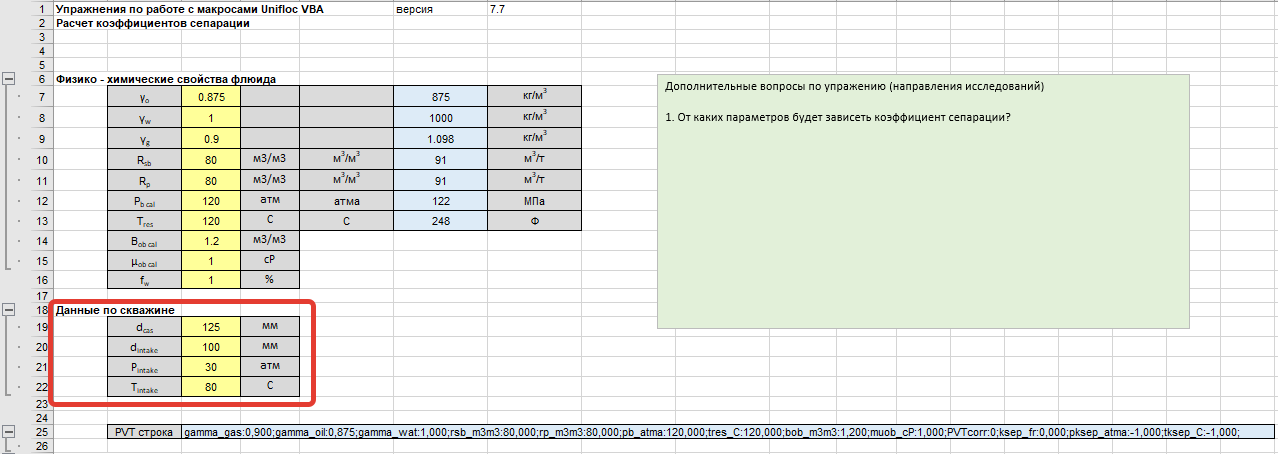
\includegraphics[width=1\linewidth]{Ex60_1}}
	\caption{Исходные данные для сепарации}
	\label{ris:Ex60_1}
\end{figure}

где

$d_{cas}$ - диаметр обсадной колонны, мм

$d_{intake}$ - диаметр приема погружного оборудования, мм

$P_{intake}$ - давление на приеме, атм

$T_{intake}$ - температура на приеме, С

Для вычисления коэффициента естественной сепарации в зависимости от дебита вставьте в ячейку E32 следующую формулу 

{ \small  \texttt{=MF\_ksep\_natural\_d(C32; wc\_; Pintake\_; Tintake\_; Dintake\_; Dcas\_; PVT\_str\_)}}

Для проведения экспериментов по влиянию изменения диаметра обсадной колонны воспользуйтесь в ячейке F32 формулой

{ \small  \texttt{=MF\_ksep\_natural\_d(C32; wc\_; Pintake\_; Tintake\_; Dintake\_; Dcas\_*cf\_dcas\_; PVT\_str\_)}}

При этом в ячейке F30 с помощью коэффициента Вы можете варьировать диаметр обсадной колонны

Для расчета доли газа в газосепараторе применяется функция

{ \small  \texttt{=MF\_gas\_fraction\_d(Pintake\_;Tintake\_;0;PVT\_str\_)*(1-F32)
}}

Коэффициент сепарации газосепаратора

{ \small  \texttt{=MF\_ksep\_gasseparator\_d(gassep\_type;G32;C32)
}}

При этом можно менять тип газосепаратора в ячейке H30

Общий коэффициент сепарации

{ \small  \texttt{=MF\_ksep\_total\_d(E32;H32)
}}

\begin{figure}[h!]
	\center{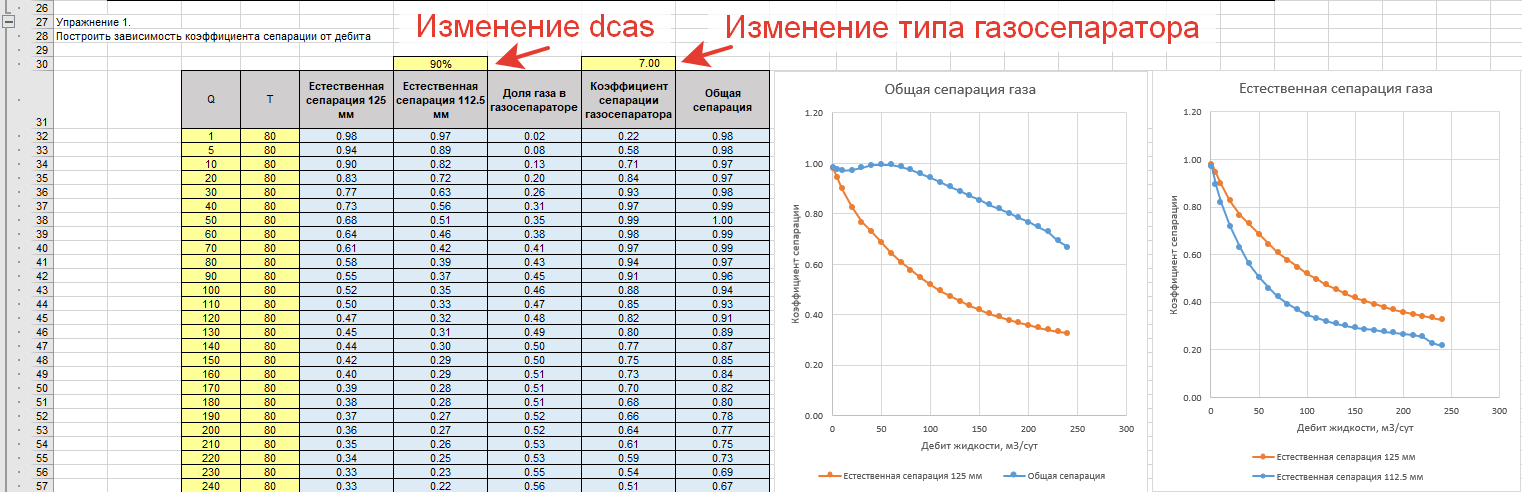
\includegraphics[width=1\linewidth]{Ex60_2}}
	\caption{Результаты расчета естественной и искусственной сепарации}
	\label{ris:Ex60_2}
\end{figure}

Вопросы к упражнению

\begin{enumerate}
	\item От каких параметров будет зависеть коэффициент сепарации?
	\item Как взаимосвязана естественная и искусственная сепарация? 
\end{enumerate}
 % Глава описание упражнений про сепарацию газа

%
\section{Анализ работы ЭЦН}

Сегодня доминирующая доля нефти в РФ добывается при помощи ЭЦН. Требуется детальное понимание основных особенностях эксплуатации данного оборудования, режимах работы, возможных осложнениях по причине высокой вязкости продукции, газосодержания, механических примесей и т.д.

Наиболее ценную информацию о работе насоса может дать его характеристика: зависимость параметров работы ЭЦН - напора, потребляемой мощности, перепада давления, КПД, от подачи (дебита скважины)

Для анализа работы скважины, оснащенной УЭЦН, требуются следующие исходные данные

\begin{enumerate}
	\item Физико - химические свойства флюида
	\item Данные по скважине
	\item Данные по ЭЦН
	\item Параметры пласта
\end{enumerate}

PVT свойства задаются аналогично предыдущим упражнениям, а для параметров, характеризующих скважину, приняты следующие обозначения

$H_{mes}$ - глубина скважины измеренная (вдоль ствола скважины), м

$H_{mes}- H_{vert}$ - удлинение ствола скважины, м

$H_{pump}$ - глубина спуска насоса, м

$ID_{cas}$ - внутренний диаметр обсадной колонны, мм

$OD_{tub}$ - внешний диаметр НКТ, мм

$ID_{tub}$ - внутренний диаметр НКТ, мм

$D_{intake}$ - диаметр приемной сетки ЭЦН, мм

$P_{buf}$ - буферное давление, атм

$P_{intake}$ - давление на приеме ЭЦН, атм

$T_{intake}$ - температура на приеме ЭЦН, С

$P_{dis}$ - давление на выкиде ЭЦН, атм

$P_{wf}$ - давление на забое, атм

$Q_{liq}$ - дебит жидкости в поверхностных условиях, м3/сут

$f_w$ - обводненность в поверхностных условиях, \%

\begin{figure}[h!]
	\center{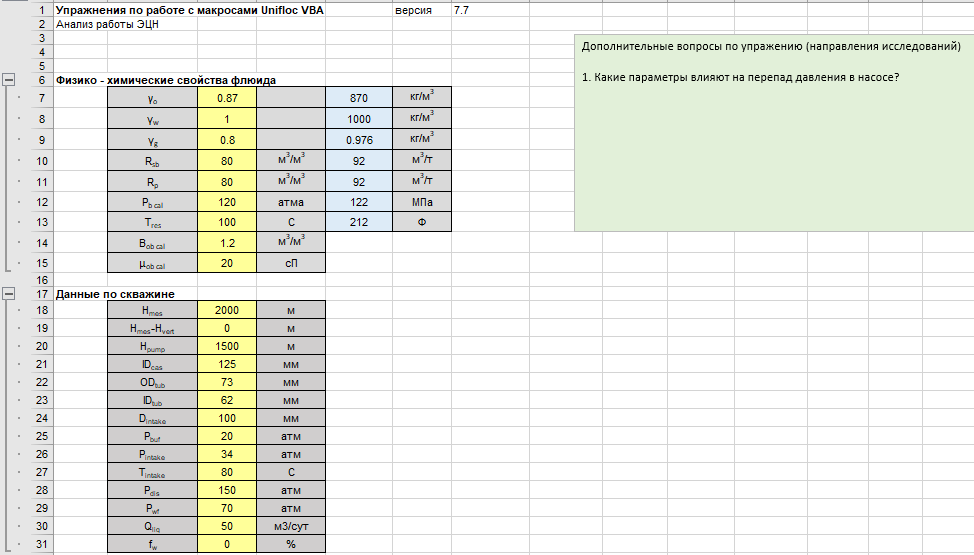
\includegraphics[width=1\linewidth]{Ex70_1}}
	\caption{Исходные данные для свойств флюида и параметров скважины}
	\label{ris:Ex70_1}
\end{figure}

Параметры, описывающие ЭЦН: 

ЭЦН $Q_{nom}$ - номинальная подача ЭЦН, м3/сут

ЭЦН $H_{nom}$ - номинальная напом ЭЦН, м

$F$ - частота питающего тока двигателя, Гц

ЭЦН $ID$ - идентификационный номер насоса (по формуле, см. ниже), находящийся в базе \unf

ЭЦН имя - обозначение насоса: название, габарит и номинальная подача (по формуле, см. ниже)

ЭЦН $Q_{max}$ - максимальная производительность насоса (по формуле, см. ниже), м3/сут

Ступени - количество ступеней, исходя из общего напора ЭЦН и напора одной ступени (по формуле, см. ниже), шт

$K_{sep_ГС}$ - коэффициент сепарации газосепаратора, \%

$P_{sep}$ - давление сепарации, атм

$T_{sep}$ - температура сепарации, С

Данные о пласте:

$P_{res}$ - пластовое давление, атм

$PI$ - коэффициент продуктивности скважины (по формуле, см. выше в упражнении IPR), м3/сут/атм

$\frac{dT}{dL}$ - геотермический градиент, град / 100 м

\begin{figure}[h!]
	\center{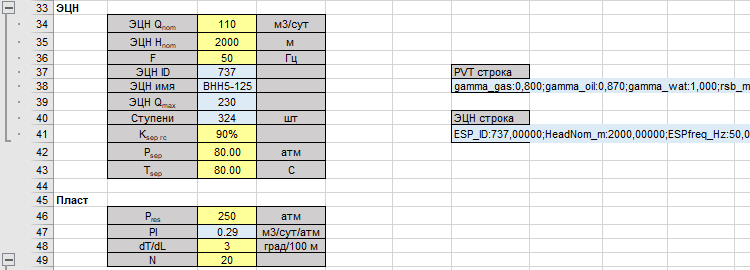
\includegraphics[width=1\linewidth]{Ex70_2}}
	\caption{Исходные данные для ЭЦН и пласта}
	\label{ris:Ex70_2}
\end{figure}

Для получения идентификационного номера насоса в базе \unf \ была использована формула

{ \small  \texttt{=ESP\_id\_by\_rate(Q\_ESP\_)}}

Для определения обозначения ЭЦН

{ \small  \texttt{=ESP\_name(C37)}}

Расчет максимально возможного дебита

{ \small  \texttt{=esp\_max\_rate\_m3day(Freq\_;PumpID\_)*1}}

Количество ступеней

{ \small  \texttt{=ЦЕЛОЕ(Head\_ESP\_/ESP\_head\_m(Q\_ESP\_;1;;PumpID\_))
}}

Также для удобства использования параметры насоса: ID, напор и рабочая частота, зашифровываются в строку с помощью функции

{ \small  \texttt{=ESP\_Encode\_string(PumpID\_;Head\_ESP\_;Freq\_)}}

Свободный газ негативно влияет на работу ЭЦН. В ячейке D51 вычисляется объемная доля газа на приеме газосепаратора с помощью формулы

{ \small  \texttt{=MF\_gas\_fraction\_d(Pintake\_;Tintake\_;fw\_;PVTstr)}}
 
В соседней ячейке D50 для удобного расположения задается вязкость в сПуаз

Построение напорной характеристики данного насоса выполняется с учетом вязкости перекачиваемой продукции. Реализованный метод пересчета характеристики с воды на вязкую жидкость Института Гидравлики позволяет учитывать изменение рабочих параметров из-за данного негативного влияния.

Для вычисления напора в метрах водного столба в ячейке D54 воспользуйтесь формулой

{ \small  \texttt{=ESP\_head\_m(C54;NumStage\_;Freq\_;PumpID\_;mu)}}

КПД ЭЦН в долях единиц 

{ \small  \texttt{=ESP\_eff\_fr(C54;NumStage\_;Freq\_;PumpID\_;mu)}}

Потребляемую ЭЦН мощность в Вт

{ \small  \texttt{=ESP\_Power\_W(C54;NumStage\_;Freq\_;PumpID\_;mu)}}

\begin{figure}[h!]
	\center{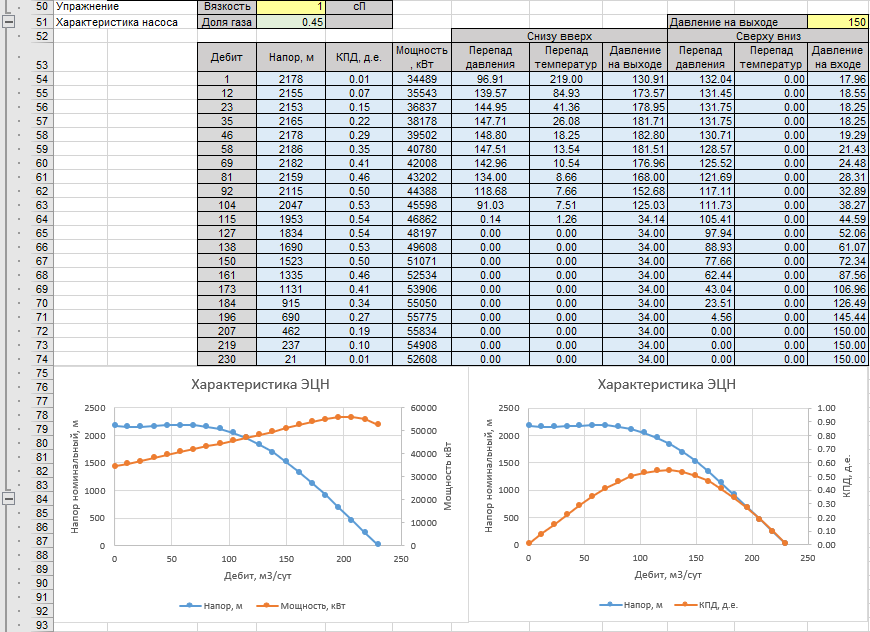
\includegraphics[width=1\linewidth]{Ex70_3}}
	\caption{Напорные характеристики ЭЦН с поправкой на вязкость}
	\label{ris:Ex70_3}
\end{figure}

Расчет перепада давления, развиваемого насосом, может происходить методом "сверху-вниз" \  и "снизу-вверх" \ , при этом расчет перепада температур только методом "снизу-вверх". Функция расчета перепада давления и температуры возвращает массив значений, т.е. одновременно перепад давления и температуры. Кроме того, входным параметром для данной функции является направление расчета. Для вычисления выделите диапазон G54:H54, наберите формулу

{ \small  \texttt{=ESP\_dP\_atm(C54; fw\_; Pintake\_; NumStage\_; Freq\_; PumpID\_; PVTstr; Tintake\_; 0)}}

и после нажмите сочетание клавиш  Ctrl+Shift+Enter. Далее протяните результат до полного заполнения двух столбцов.

Зная давление на приеме и перепад давления в ЭЦН, давление на выходе ЭЦН можно легко посчитать по формуле

{ \small  \texttt{=G54+Pintake\_}}

Предварительно задав давление на выходе ЭЦН в ячейке L51 возможно посчитать перепад давления методом "сверху-вниз"\ аналогичным образом по формуле

{ \small  \texttt{=ESP\_dP\_atm(C54; fw\_; Pdis\_; NumStage\_; Freq\_; PumpID\_; PVTstr; Tintake\_; Tintake\_; 0)}}

И давление на входе, зная давление на выходе и перепад давления

{ \small  \texttt{=Pdis-J54}}

\begin{figure}[h!]
	\center{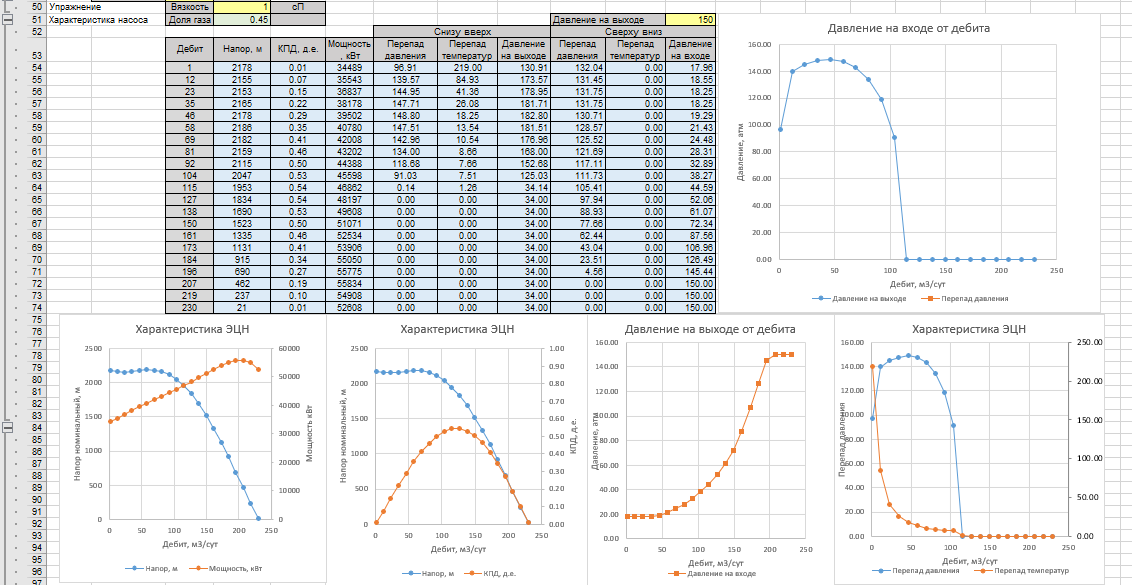
\includegraphics[width=1\linewidth]{Ex70_4}}
	\caption{Расчет перепада давления и температур в ЭЦН в зависимости от дебита}
	\label{ris:Ex70_4}
\end{figure}

Вопросы для упражнения:

\begin{enumerate}
	\item Какие параметры влияют на перепад давления в насосе?
	\item Насколько сильно влияет вязкость на напорные характерситики ЭЦН?
	\item Как влияет на работу ЭЦН изменение частоты?
\end{enumerate}


\section{Анализ работы ПЭД}

Упражнение показывает характеристики погружного асинхронного электрического двигателя, применяемого в УЭЦН.

Также стоит отметить, что расчетные функции предназначаются для образовательных целей. Детального сопоставления расчетных характеристик с фактическими не проводилось. (06.2019)

Для выполнения упражнения необходимо задать параметры электродвигателя

$U_{nom}$ - номинальное напряжение ПЭД, В

$F_{nom}$ - номинальная частота тока, Гц

$I_{nom}$ - номинальная сила тока, А

$ID$ - способ инициализации данных двигателя. 1 - по фактическим значениям параметров (по паспорту), 2 - по схеме замещения Гридина

А также рабочее напряжение $U$, В и рабочую частоту тока $F$, Гц

После этого в ячейке С10 будет произведен расчет номинальной мощности ПЭД с помощью функции

{ \small  \texttt{=Motor\_Pnom\_kW(Unom;Inom;Fnom;ID)}}

\begin{figure}[h!]
	\center{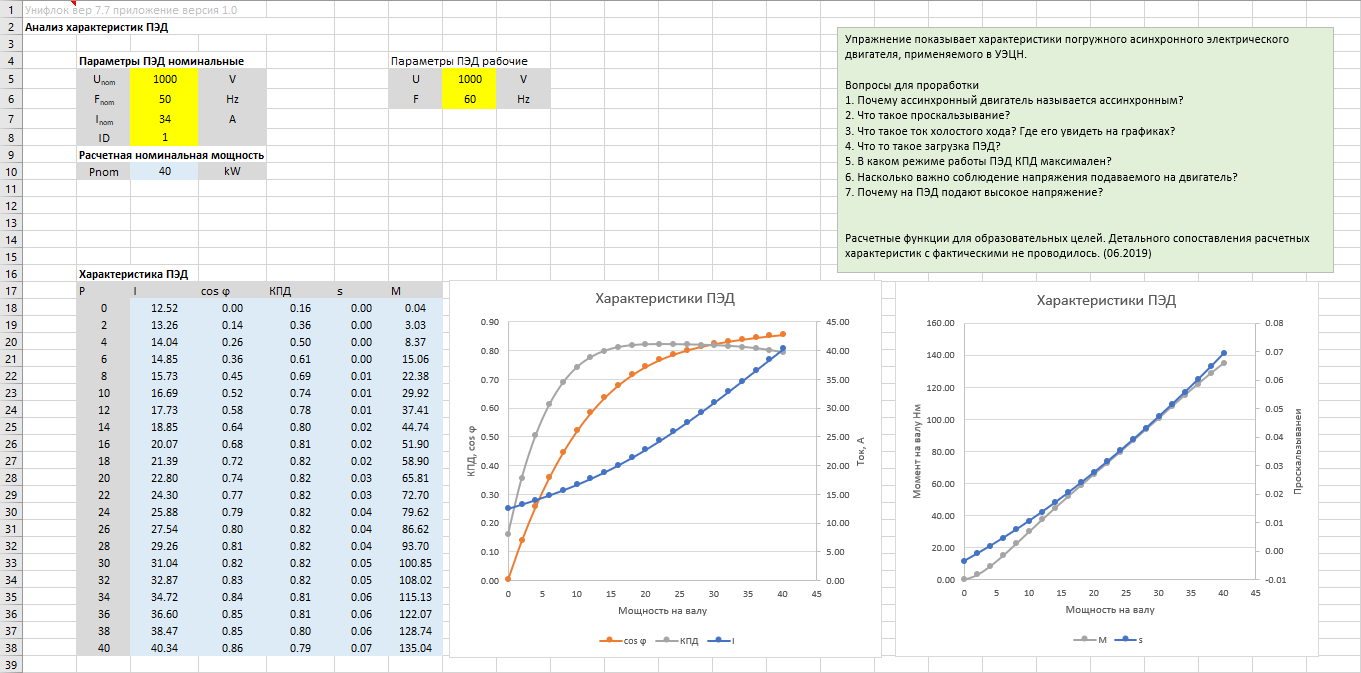
\includegraphics[width=1\linewidth]{Ex80_1}}
	\caption{Исходные данные ПЭД и различные характеристики в зависимости от мощности на валу}
	\label{ris:Ex80_1}
\end{figure}

Для построения характеристики ПЭД (параметры двигателя от мощности на валу $M$) воспользуйтесь следующими формулами

Определение тока двигателя $I$, A

{ \small  \texttt{=motor\_I\_A(B18;F;U;Unom;Inom;Fnom;ID)}}

Расчет $cos \varphi $

{ \small  \texttt{=motor\_CosPhi\_d(B18;F;U;Unom;Inom;Fnom;ID)}}

КПД, д.ед.

{ \small  \texttt{=motor\_Eff\_d(B18;F;U;Unom;Inom;Fnom;ID)}}

Проскальзывание $S$

{ \small  \texttt{=motor\_S\_d(B18;F;U;Unom;Inom;Fnom;ID)}}

Момент на валу $M$, Н*м

{ \small  \texttt{=motor\_M\_Nm(B18;F;U;Unom;Inom;Fnom;ID)}}

\begin{figure}[h!]
	\center{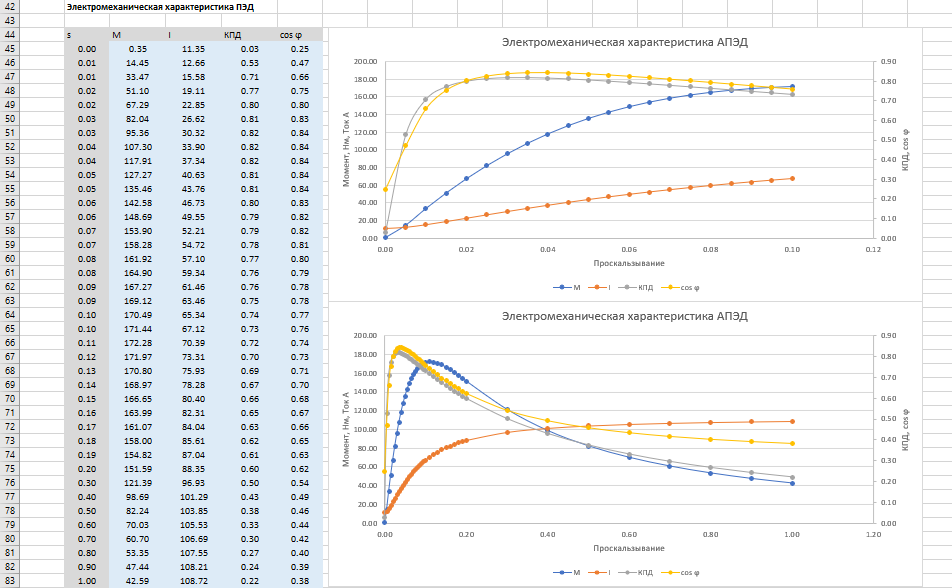
\includegraphics[width=1\linewidth]{Ex80_2}}
	\caption{Электромеханическая характеристика АПЭД}
	\label{ris:Ex80_2}
\end{figure}

Для расчета электромеханической характеристики АПЭД (параметры двигателя в зависимости от проскальзывания $S$) используйте формулы

Момент на валу $M$, Н*м 

{ \small  \texttt{=motor\_M\_slip\_Nm(B45;F;U;Unom;Inom;Fnom;0)}}

Сила тока $I$, А

{ \small  \texttt{=motor\_I\_slip\_A(B45;F;U;Unom;Inom;Fnom;0)}}

КПД, д.ед.

{ \small  \texttt{=motor\_Eff\_slip(B45;F;U;Unom;Inom;Fnom;0)}}

Расчет $cos \varphi $

{ \small  \texttt{=motor\_CosPhi\_slip(B45;F;U;Unom;Inom;Fnom;0)}}


\begin{figure}[h!]
	\center{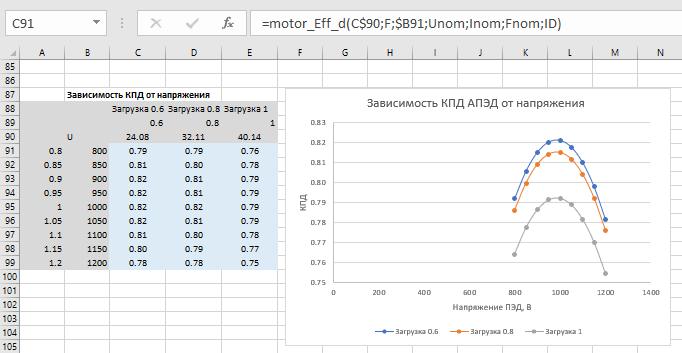
\includegraphics[width=1\linewidth]{Ex80_3}}
	\caption{Зависимость КПД АПЭД от напряжения и загрузки}
	\label{ris:Ex80_3}
\end{figure}

Для проведения исследований по напряжению ПЭД воспользуйтесь следующими формулами для значений загрузки двигателя 0.6, 0.8, 1 

{ \small  \texttt{=motor\_Eff\_d(C\$90;F;\$B91;Unom;Inom;Fnom;ID)}}

{ \small  \texttt{=motor\_Eff\_d(D\$90;F;\$B91;Unom;Inom;Fnom;ID)}}

{ \small  \texttt{=motor\_Eff\_d(E\$90;F;\$B91;Unom;Inom;Fnom;ID)}}

в ячейках C91, E91, D91 соответственно. "Протянув"\ значения Вы можете заполнить таблицу.

Вопросы для упражнения:

\begin{enumerate}
	\item Почему ассинхронный двигатель называется ассинхронным?
	\item Что такое проскальзывание?
	\item Что такое ток холостого хода? Где его увидеть на графиках?
	\item Что то такое загрузка ПЭД?
	\item В каком режиме работы ПЭД КПД максимален?
	\item Насколько важно соблюдение напряжения подаваемого на двигатель?
	\item Почему на ПЭД подают высокое напряжение?
\end{enumerate} % Глава описание упражнений про ЭЦН

%

\section{Анализ работы фонтанирующей скважины}

При достаточном количестве естественной энергии скважина может фонтанировать. Инженерные расчеты требуются как для оптимизации работы самого подъемника, так и системы "скважина-пласт".

Для упражнения требуется задать PVT свойства флюидов, конструкцию скважины, свойства пласта и текущий режим работы скважины (дебит). Все исходные данные заполняются аналогично предыдущим упражнениям за исключением функции, объединяющей все данные о скважине в одну строку, расположенной в ячейке  $G23$

{ \small  \texttt{=well\_encode\_string(Hmes\_;Htube\_;Udl\_;Dcas\_;Dtub\_;0;;Twf\_;Tbuf\_)
}}

\begin{figure}[h!]
	\center{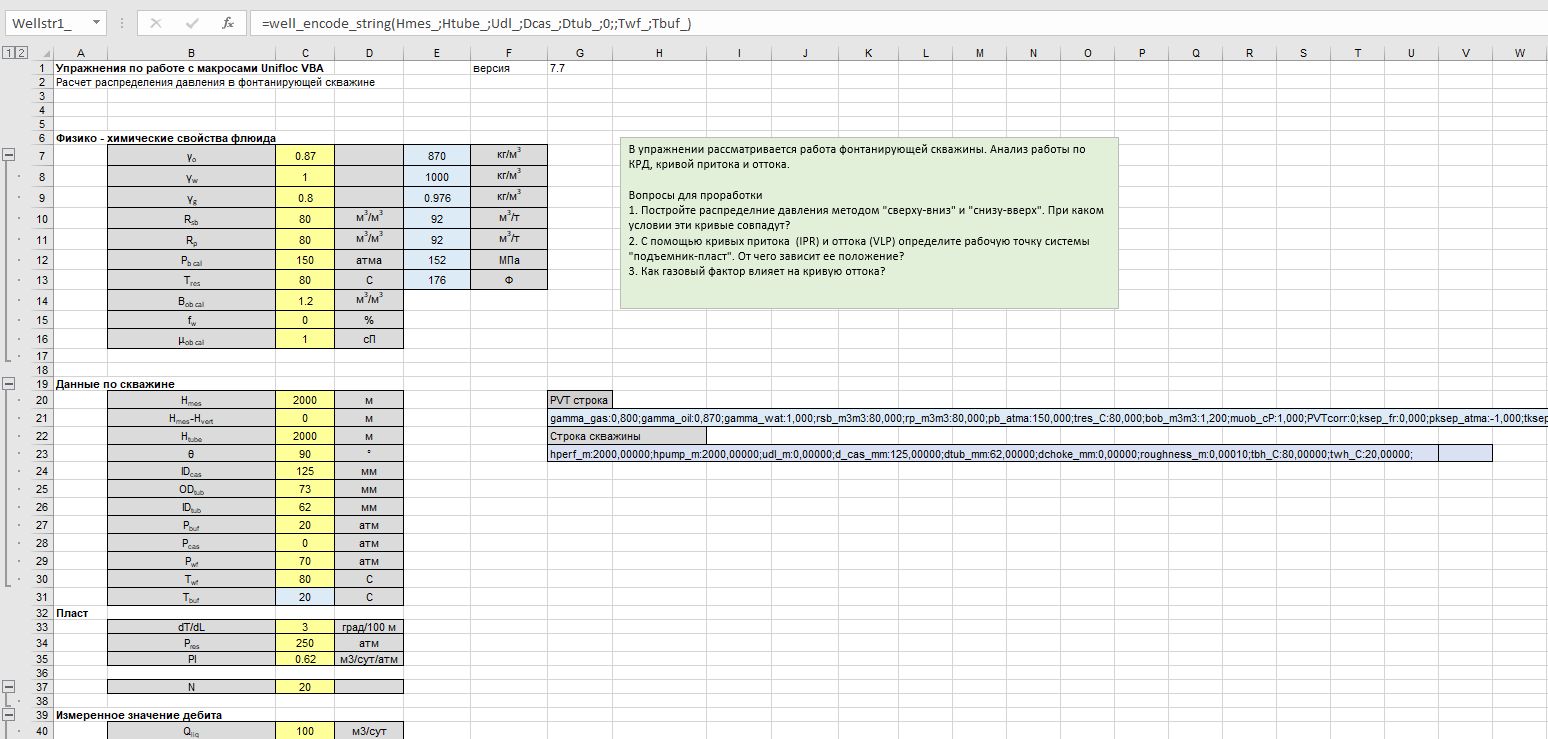
\includegraphics[width=1\linewidth]{Ex90_1}}
	\caption{Исходные данные для расчета фонтанирующей скважины}
	\label{ris:Ex90_1}
\end{figure}

В первой части задания требуется построить распределение давления в скважине методом сверху-вниз и снизу-вверх, задавая при этом граничные условия - давление на устье и на забое соответственно. Для расчета воспользуйтесь в ячейке $E50$ функцией

{ \small  \texttt{=MF\_p\_pipe\_atma(Qtest\_; fw\_;C49; C50;E49;PVRstr1\_; theta\_;Dtub\_;;D49;D50)
}}

"протянув"\ ее на весь столбец. Расчет снизу-вверх выполните аналогичным образом. Обратите внимание, что при правильных расчетах КРД должны совпадать - решение не должно зависеть от направления.

\begin{figure}[h!]
	\center{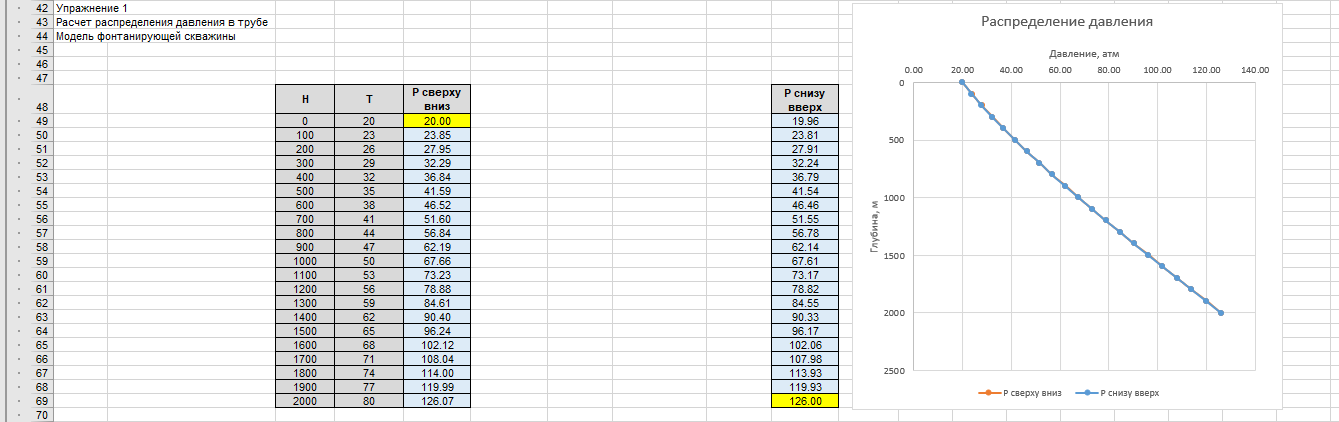
\includegraphics[width=1\linewidth]{Ex90_2}}
	\caption{Расчет КРД в фонтанирующей скважине}
	\label{ris:Ex90_2}
\end{figure}

Во второй части упражнения необходимо построить кривую притока (индикаторную кривую, по Вогелю) и кривую оттока (зависимость давления в начале подъемной трубы от дебита при неизменном давление на выходе). Забойное давление принимается равным рассчитанному из предыдущей части упражнения. Максимальный дебит скважины и коэффициент продуктивности можно варьировать вместе с обводненностью продукции скважины для анализа добывающей системы. Точка пересечения кривых притока и оттока будет являться рабочей точкой системы "пласт-скважина".

Для вычисления забойного давления для индикаторной кривой воспользуйтесь в ячейке $F78$ уже знакомой Вам функцией

{ \small  \texttt{=IPR\_Pwf\_atma(PI\_1;Pres\_;E78;fw\_;Pb\_)}}

Расчет забойного давления по устьевому в ячейке $G78$ примените функцию
 
{ \small  \texttt{=well\_pwf\_plin\_atma(E78;fw\_;Pbuf\_; Pcas\_; Wellstr1\_; PVRstr1\_; ;1;;;;;;1)}} 

Для другой величины обводненности продукции в $H78$ при анализе дальнейшей работы

{ \small  \texttt{=well\_pwf\_plin\_atma(E78;fw\_2;Pbuf\_; Pcas\_; Wellstr1\_; PVRstr1\_; ;1;;;;;;1)}} 

Заполнив таблицу до конца Вы получите следующий результат

\begin{figure}[h!]
	\center{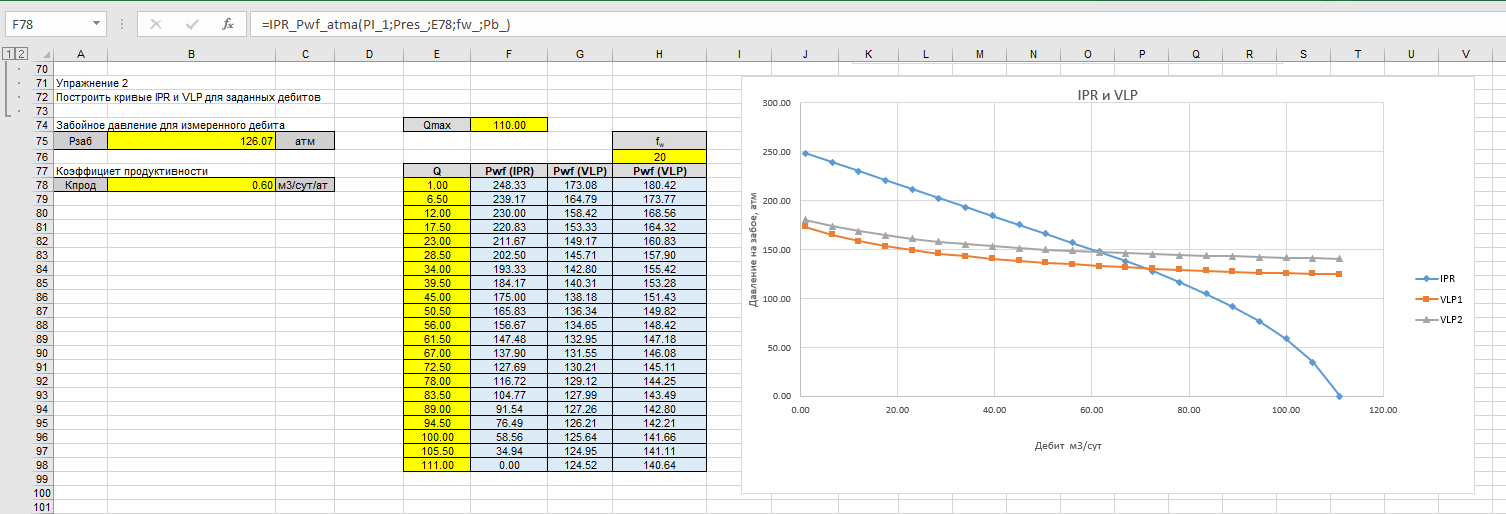
\includegraphics[width=1\linewidth]{Ex90_3}}
	\caption{Кривые оттока и притока для узлового анализа работы фонтанирующей скважины}
	\label{ris:Ex90_3}
\end{figure}

Для анализа влияния ГФ скважины на забойное давление воспользуйтесь теми же самыми функциями, за исключением того, что каждый раз будет меняться PVT строка свойств флюидов

В ячейке $H108$ 

{ \small  \texttt{=well\_pwf\_plin\_atma(Qtest\_;fw\_;Pbuf\_;Pcas\_;Wellstr1\_;G108;;1;;;;;;1)}}

В ячейке $I108$ 

{ \small  \texttt{=well\_pwf\_plin\_atma(Qtest\_;fw\_3;Pbuf\_;Pcas\_;Wellstr1\_;G108;;1;;;;;;1)}}

\begin{figure}[h!]
	\center{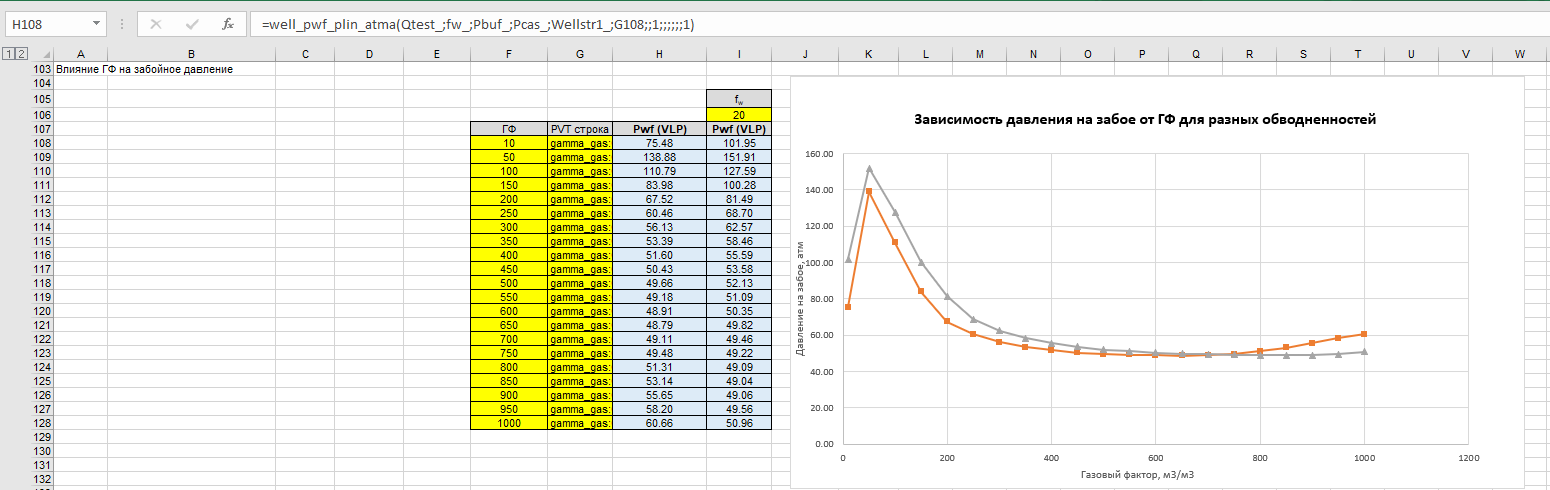
\includegraphics[width=1\linewidth]{Ex90_4}}
	\caption{Влияние газового фактора и обводненности на забойное давление}
	\label{ris:Ex90_4}
\end{figure}

Теперь Вы можете ответить на вопросы:

Вопросы для проработки

\begin{enumerate}
	\item Постройте распределние давления методом сверху-вниз и снизу-вверх. При каком условии эти кривые совпадут?
	\item С помощью кривых притока  (IPR) и оттока (VLP) определите рабочую точку системы "скважина-пласт". От чего зависит ее положение?
	\item Как газовый фактор влияет на кривую оттока?
\end{enumerate}

\section{Анализ работы скважины, оснащенной УЭЦН}

По сравнению с моделью фонтанирующей скважины в данный расчет добавляются такие важные элементы, как сепарация на приеме погружного оборудования и напорная характеристика ЭЦН. К стандартным исходным данным добавляется вторая PVT строка ($G45$) для разделения упражнения на 2 части. 

{ \small  \texttt{=PVT\_encode\_string(gamma\_gas\_; gamma\_oil\_; ; Rsb\_; Rp\_; Pb\_; Tres\_; Bob\_; mu\_;; KsepGasSep\_; PKsep2; TKsep2)
}}

Стоит сразу отметить важность определения давления и температуры, при которой происходит сепарация газа в затрубное пространство. При неизвестном давлении на приеме погружного оборудования (давлении сепарации) требуется определить его с помощью гидравлической корреляции, например, при расчете снизу-вверх от забойного давления. Однако расчет перепада давления в трубе зависит от PVT свойств, в том числе давления сепарации - поэтому требуется итеративный подход для изменения давления сепарации до тех пор, пока оно не окажется стабильным (и равным давлению на приеме погружного оборудования по гидравлической корреляции). Т.к. при сепарации происходит модификация флюида, пренебрежение согласованностью приведет к неправильному расчету - поток может быть дегазированным на забое или наоборот с высокой долей газа в насосе или НКТ. Изменять давление сепарации $P_{sep}$ можно в ячейке $C43$

\begin{figure}[h!]
	\center{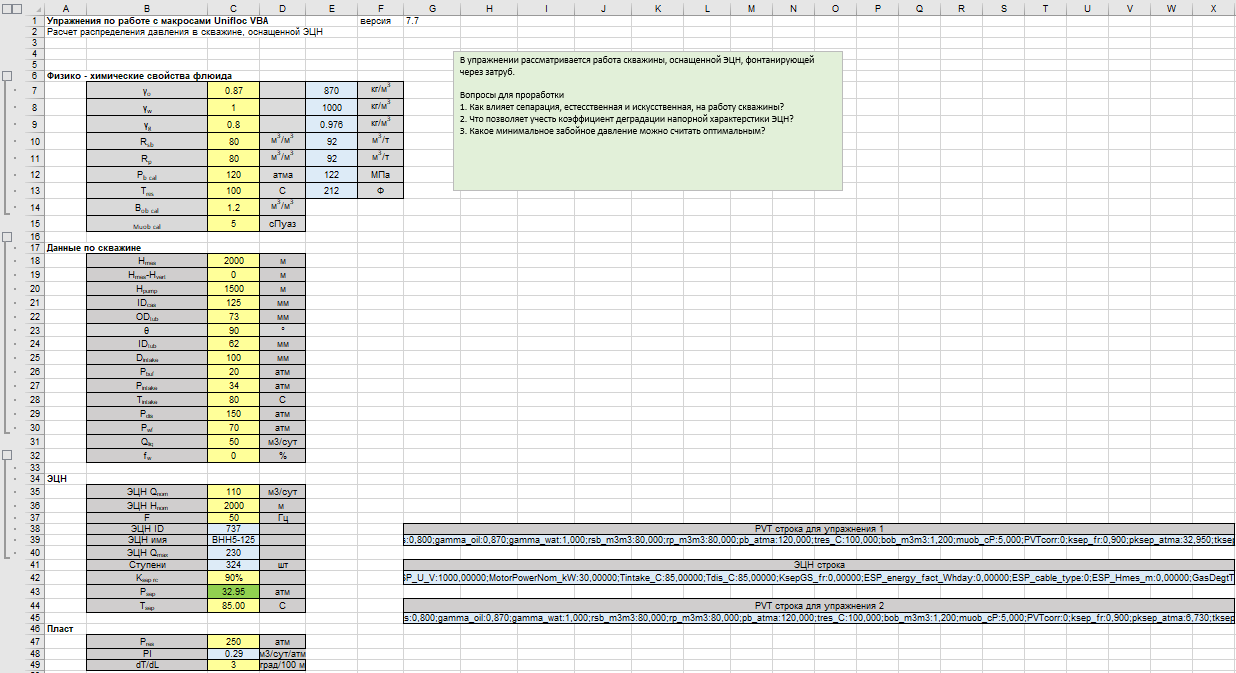
\includegraphics[width=1\linewidth]{Ex100_1}}
	\caption{Исходные данные для расчета скважины, оснащенной УЭЦН}
	\label{ris:Ex100_1}
\end{figure}

В первой части упражнения предлагается построить распределение давления в скважине с постоянным дебитом. 

Кривую давления от забоя до приема можно получить с помощью функции

{ \small  \texttt{=MF\_p\_pipe\_atma(Q\_;fw\_;C83;C82; F83;PVT\_str\_; theta\_; Dtub\_;; D83;D82)
}}

"протянув"\ ее до глубины спуска оборудования. С учетом сепарации, которая подробно описывалась выше, требуется изменять значение давления сепарации $P_{sep}$ в исходных данных ($C43$) пока оно не станет равным расчетному.

Затем в ячейке $G78$ можно определить коэффициент естественной сепарации

{ \small  \texttt{=MF\_ksep\_natural\_d(Q\_; wc\_; Pintake\_; Tintake\_; Dintake\_; Dcas\_; PVT\_str\_)
}}

А в $H78$ искусственную с помощью 

{ \small  \texttt{=MF\_ksep\_total\_d(G78;KsepGasSep\_)
}}

Распределение давления в НКТ рассчитывается методом сверху-вниз, начиная с ячейки $K64$

{ \small  \texttt{=MF\_p\_pipe\_atma(Q\_;fw\_;C63;C64;K63;PVT\_str\_;theta\_;Dintake\_;;D63;D64)
}}

Таким образом можно получить перепад давления в насосе не прибегая к расчету самого насоса - он будет равен разнице между давлением в нижней точке НКТ и на приеме погружного оборудования (ячейка $N78$). Но по напорной характеристике с помощью функции в $M78$

{ \small  \texttt{=ESP\_dP\_atm(Q\_; fw\_;Pintake\_; NumStage\_;Freq\_; PumpID\_; PVT\_str\_;Tintake\_; 0;1;;D60)
}}

также можно получить данное значение, воспользовавшись коэффициентом деградации напорной характеристики ЭЦН в $D60$ для адаптации модели. При совпадении результатов двух независимых расчетов возможно оценить состояние погружного оборудования.

Полезным для анализа работы добывающей системы будет знание о доли газа в потоке как до приема погружного оборудования (начиная с ячейки $I83$)

{ \small  \texttt{=MF\_gas\_fraction\_d(F83;D83;fw\_;PVT\_str\_)
}}

так и после сепарации в НКТ (с $J78$)

{ \small  \texttt{=MF\_gas\_fraction\_d(K78;D78;fw\_;PVT\_str\_)
}}

На этом первая часть упражнения завершается.

\begin{figure}[h!]
	\center{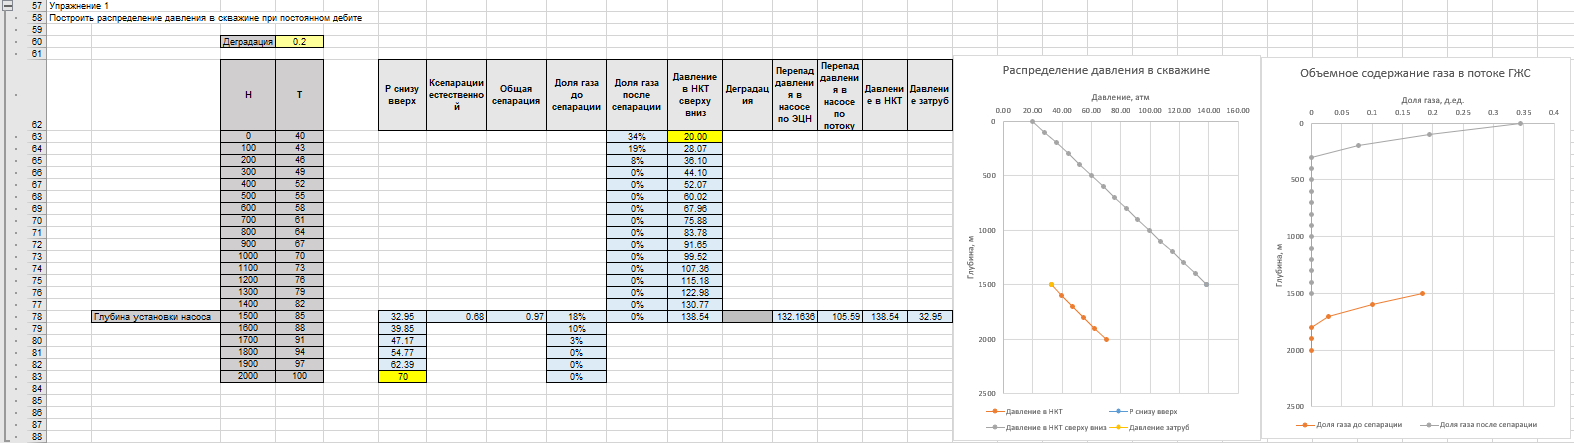
\includegraphics[width=1\linewidth]{Ex100_2}}
	\caption{Распределение давления в скважине с постоянным дебитом}
	\label{ris:Ex100_2}
\end{figure}

Во второй части упражнения распределение давления скважины строится с учетом того, что она имеет постоянную продуктивность. Изменение забойного давления в ячейке $D92$ приведет к изменению дебита скважины. Также могут варьироваться давление сепарации, коэффициент деградации и частота ЭЦН для настройки модели.

Сам расчет ведется только методом снизу-вверх: по забойному давлению определяется давление на приеме, затем вместе с коэффициентом сепарации рассчитывается перепад давления в насосе по напорной характеристике, а после устьевое давление по давлению на выходе насоса, начиная с ячейки $K114$ c помощью функции

{ \small  \texttt{=MF\_p\_pipe\_atma(Qreal\_; fw\_;C115;C114; K115;PVT\_str\_2;theta\_; Dintake\_;; D115; D114)
}}

При этом PVT строка будет использоваться другая из-за отличных значений давления на приеме по сравнению с первой частью упражнения.

\begin{figure}[h!]
	\center{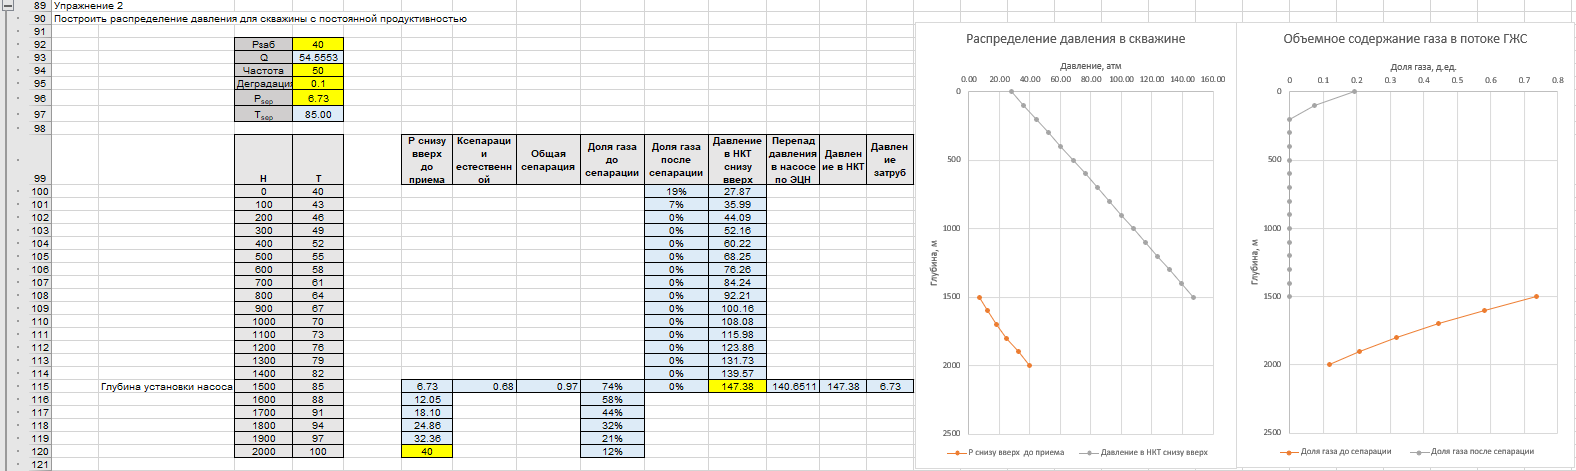
\includegraphics[width=1\linewidth]{Ex100_3}}
	\caption{Распределение давления в скважине с постоянной продуктивностью}
	\label{ris:Ex100_3}
\end{figure}

С помощью дополнительных исследований (при необходимости) ответьте на вопросы

\begin{enumerate}
	\item Как влияет сепарация, естественная и искусственная, на работу скважины?
	\item Что позволяет учесть коэффициент деградации напорной характеристики ЭЦН?
	\item Какое минимальное забойное давление можно считать оптимальным?
\end{enumerate}


\section{Анализ работы скважины, оснащенной ЭЦН, фонтанирующей через затрубное пространство}

Общая теория 

При спуске погружного оборудования в фонтанирующую скважину с большим газовым фактором газожидкостный поток у приема может разделяться на 2 составляющие: поток с низким газосодержанием после сепарации естественной и искусственной в НКТ и поток с большой долей свободного газа в затрубное пространство. 

При этом ЭЦН за счет энергии движения ГЖС работает практически на холостом ходу, развивая обычный перепад давления по напорной характеристике. Также при дебите большем, чем максимально возможный перепад давления  насоса, может происходить турбинное вращение, насос будет работать как гидравлическое сопротивление. Перегрев электродвигателя не происходит, т.к. он непрерывно охлаждается общим газожидкостным потоком.

В затрубном пространстве за счет большого количество газа будет происходить фонтанирование. Давление в затрубном пространстве будет большим, чем буферное, потому как обратный клапан в затрубе, предназначеныый для сброса газа, с жидкостью будет функционировать как штуцер, дросселируя давление. Без обратного клапана можно сделать  логичное предположение о том, что давления будут равными - газлифтный эффект в затрубном пространстве (подъем газожидкостной смеси за счет снижения плотности) будет равен перепаду давления, который создает ЭЦН.

Отсюда возникает вопрос, рационально ли устанавливать ЭЦН в фонтанирующую скважину с большим газовым фактором?

В данном упражнении предлагается смоделировать данный процесс. Но Вы также можете просмотреть расширенный расчет реальной скважины в папке "аpp".

\begin{figure}[h!]
	\center{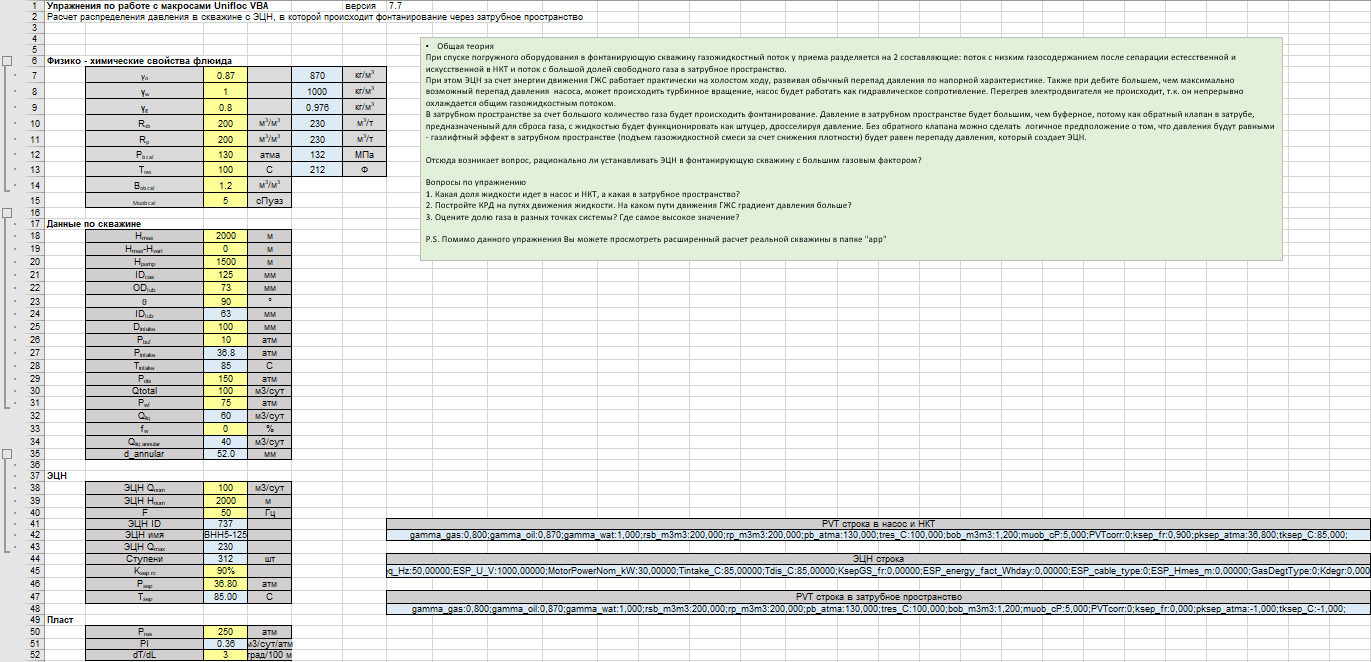
\includegraphics[width=1\linewidth]{Ex110_1}}
	\caption{Набор исходных данных, для расчета фонтанирования через затрубное пространство}
	\label{ris:Ex110_1}
\end{figure}

Процесс моделирования добывающей системы осложняется тем, что неизвестны доли жидкости: поступающая в насос и НКТ и поднимающаяся по затрубному пространству. Для этого введем коэффициент деления потока ГЖС, обозначающий долю жидкости, поступающую в насос и НКТ, в ячейке $N63$. Расчет распределения давления в НКТ и затрубном пространстве будем вести стандартным образом с помощью гидравлических корреляций. Отличия в определении давления будет выражаться в применении двух PVT строк: в ячейке $G42$ будет флюид, учитывающий сепарацию на приеме погружного оборудования, он будет описывать поведение ГЖС в НКТ, а в ячейке $G48$ будет флюид без сепарации - весь газ будет оставаться в потоке в затрубном пространстве; с помощью коэффициента деления потока из общего дебита $Q_{total}$ рассчитывается расход по НКТ $Q_{liq}$ и по затрубному  пространству $Q_{liq annular}$

К формулам, используемым в предыдущем упражнении, добавляется расчет давления в затрубном пространстве (с $Q80$)

{ \small  \texttt{=MF\_p\_pipe\_atma(Q\_annular\_; fw\_; C81;C80; Q81; PVT\_str\_annular\_; theta\_; d\_annular\_pr; 1;D81;D80)
}}

И соответственно доля газа в ГЖС затрубного пространства (с $J81$) 

{ \small  \texttt{=MF\_gas\_fraction\_d(Q81; D81; fw\_; PVT\_str\_annular\_)
}}

Также напомним о важности правильно определения давления сепарации (описано выше). 

Таким образом, с помощью КРД в затрубном пространстве и НКТ предлагается найти такие параметры системы (изменяя коэффициент деления потока, коэффициент деградации напорной характеристики насоса и т.д.) при котором давление в затрубном пространстве будет равным или большим, чем буферное давление.

\begin{figure}[h!]
	\center{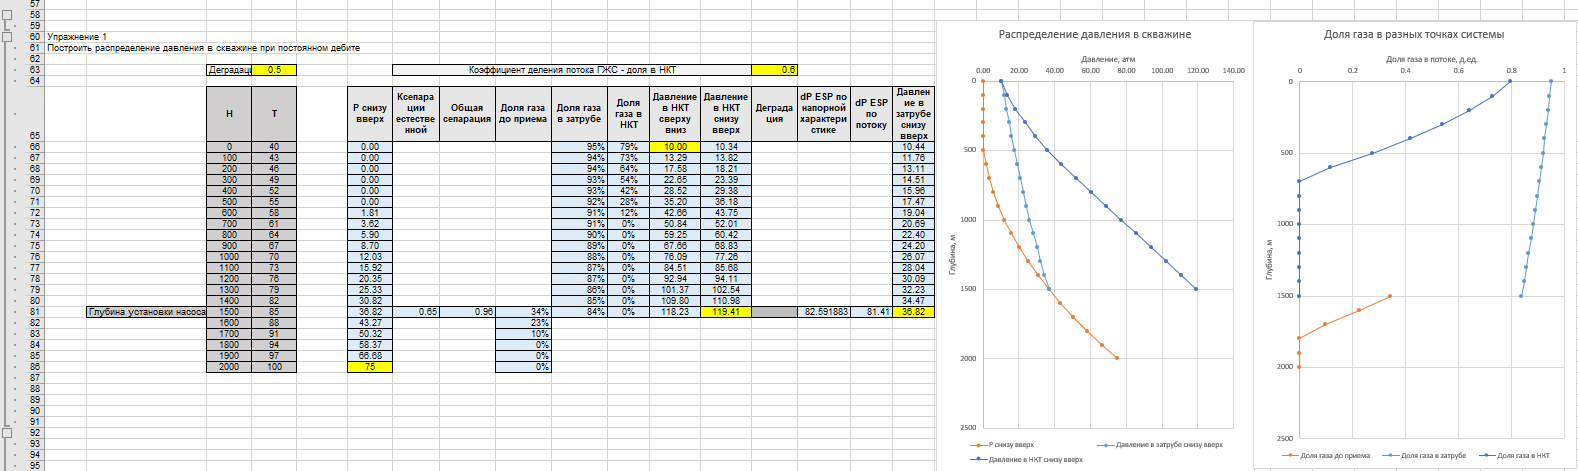
\includegraphics[width=1\linewidth]{Ex110_2}}
	\caption{Настроенная модель скважины с равными давлениями на устье}
	\label{ris:Ex110_2}
\end{figure}

Вопросы по упражнению
\begin{enumerate}
	\item  Какая доля жидкости идет в насос и НКТ, а какая в затрубное пространство?
	\item  Постройте КРД на путях движения жидкости. На каком пути движения ГЖС градиент давления больше?
	\item Оцените долю газа в разных точках системы? Где самое высокое значение?
	\item Оптимальнее ли будет эксплуатировать скважину с помощью чисто фонтанного способа добычи?
\end{enumerate} % Глава описание упражнений про скважину











\section{Набор расчетных модулей анализа скважины}
Пример использования алгоритмов \unf   приведен в файле \texttt{UF7\_calc\_well.xlsm}.

Файл содержит набор расчетных модулей позволяющих провести анализ данных описывающих работу скважины с применением различных методов добычи.

\subsection{Расчетный модуль анализа и настройки PVT свойств}

 % Глава описание упражнений
%	\chapter*{Заключение}                       % Заголовок

Заключение возможно будет тут когда то      % Заключение
%	\chapter*{Единицы измерений} % Заголовок
\addcontentsline{toc}{chapter}{Единицы измерений}  % Добавляем его в оглавление
\noindent

\section*{Давление}
 
 atm, атм "--- физическая атмосфера 
 
 atma, атма "--- абсолютное значение величины в атмосферах
 
 atmg, атми "--- избыточное (измеренное) значение величины в атмосферах. отличается от абсолютной на величину атмосферного давления (1.01325 атма)

\chapter*{Список сокращений и условных обозначений} % Заголовок
\addcontentsline{toc}{chapter}{Список сокращений и условных обозначений}  % Добавляем его в оглавление
\noindent

$\gamma_g$  - \mintinline{vb.net}{gamma_gas} - удельная плотность газа, по воздуху. 

$\gamma_o$  - \mintinline{vb.net}{gamma_oil} - удельная плотность нефти, по воде.

$\gamma_w$  - \mintinline{vb.net}{gamma_wat}- удельная плотность воды, по воде. 

$R_{sb}$ - \mintinline{vb.net}{Rsb_m3m3} газосодержание при давлении насыщения,  $\text{м}^3/\text{м}^3$. 

$R_p$ - \mintinline{vb.net}{Rp_m3m3}. замерной газовый фактор, $\text{м}^3/\text{м}^3$.

$P_b$ - \mintinline{vb.net}{Pb_atma}. давление насыщения, атма.  

$T_{res}$ - \mintinline{vb.net}{Tres_C} пластовая температура, \textcelsius. 

$B_{ob}$ - \mintinline{vb.net}{Bob_m3m3} объёмный коэффициент нефти,  $\text{м}^3/\text{м}^3$. 

$\mu_{ob}$ - \mintinline{vb.net}{Muob_cP}. вязкость нефти при давлении насыщения, сП. 

$Q_{liq}$ - \mintinline{vb.net}{Qliq_scm3day}. дебит жидкости измеренный на поверхности (приведенный к стандартным условиям), м3/сут. 

$f_{w}$ - \mintinline{vb.net}{fw_perc, fw_fr} объёмная обводненность (fraction of water), проценты или доли единиц. 

$f_{g}$ - \mintinline{vb.net}{fg_perc, fg_fr} объёмная доля газа в потоке (fraction of gas), проценты или доли единиц. 

$PI$ - \mintinline{vb.net}{pi_sm3dayatm} - коэффициент продуктивности скважины, $\text{м}^3$/сут/атм

$\rho_{air}$ - \mintinline{vb.net}{rho_air} - плотность воздуха, относительная плотность газа $\gamma_g$ считается по воздуху $\rho_{air} = 1.22$ кг/$\text{м}^3$        % Список сокращений и условных обозначений
%	\chapter*{Словарь терминов}             % Заголовок
\addcontentsline{toc}{chapter}{Словарь терминов}  % Добавляем его в оглавление

Словарь описывает термины и сокращения широко используемые в описании и в системе \unf.


\textbf{VBA} "--- Visual Basic for Application язык программрования встроенный в Excel и использованный для написания макросов \unf.

\textbf{VBE} "--- Среда разработки для языка VBA. Встроена в Excel.

\textbf{BHP, Pwf} "--- Bottom hole pressure. Well flowing pressure. Забойное давление

\textbf{BHT, TBH} "--- Bottom hole temperature. Забойная температура

\textbf{WHP, PWH} "--- Well head pressure. Устьевое давление. Как правило, соответствует буферному давлению.

\textbf{WHT, TWH} "--- Well head temperature. Устьевая температура. Температура флюида на устье скважины. Температура в точке замера буферного давления.

\textbf{IPR} "--- Inflow performance relationship. Индикаторная кривая. Зависимость забойного давления от дебита для пласта. Широко используется в узловом анализе.

\textbf{VLP, VFP} "--- Vertical lift performance, vertical flow performance, outflow curve. Кривая лифта, кривая оттока. Зависимость забойного давления от дебита для скважины. Широко используется в узловом анализе.

\textbf{ESP} "--- Electrical submersible pump. Электрический центробежный насос.

\textbf{GL} "--- Gas Lift. Газлифтный способ эксплуатации добывающих скважин. 

\textbf{РНХ ЭЦН} "--- Расходно напорная характеристика электрического центробежного насоса. Ключевая характеристика ЭЦН. Дается производителем в каталоге ЭЦН для новых насосов или определяется на стенде для ремонтных ЭЦН. 

\textbf{PVT} "--- Pressure Volume Temperature. Общепринятое обозначение для физико-химических свойств пластовых флюидов - нефти, газа и воды.

\textbf{MF} "--- MultiPhase. Много Фазный поток. Префикс для функций имеющих дело с расчетом многофазного потока в трубах и скважине.

\textbf{НКТ} "--- Насосно компрессорная труба. Часть конструкции скважины. по колонне НКТ добывается скважинная продукция или закачивается вода. Может быть заменена в процессе эксплуатации при ремонте скважины. 

\textbf{ЭК} "--- Эксплуатационная колонна. Часть конструкции скважины.  Не может быть заменена в процессе эксплуатации при ремонте скважины. 

\textbf{ГЖС} "--- Газо жидкостная смесь. Часто используется для обозначения совместно двигающихся флюидов в многофазном потоке - нефти, газа, воды.

\textbf{Барботаж, ZNLF} "--- Движение газа через неподвижный столб жидкости. ZNLF - zero net liquid flow. Встречается в скважинах с насосами - в межтрубном пространстве газ движется через неподвижный столб жидкости. Влияет на динамический уровень в скважине.

\textbf{ЭЦН} "--- Электрический центробежный насос.

\textbf{УЭЦН} "--- Установка электрического центробежного насоса. Включает весь комплекс погружного и поверхностного оборудования необходимого для работы насоса - насос (ЭЦН), погружной электрический двигатель (ПЭД), гидрозащита (ГЗ), входной модуль (ВМ) и газосепаратор (ГС), электрический кабель, станция управления (СУ) и другие элементы

\textbf{ЧРП} "--- Частотно регулируемый привод. Элемент УЭЦН обеспечивающий возможность вращения вала УЭЦН с различными частотами.      % Словарь терминов
	\clearpage                                  % В том числе гарантирует, что список литературы в оглавлении будет с правильным номером страницы
%\hypersetup{ urlcolor=black }               % Ссылки делаем чёрными
%\providecommand*{\BibDash}{}                % В стилях ugost2008 отключаем использование тире как разделителя 
\urlstyle{rm}                               % ссылки URL обычным шрифтом
\ifdefmacro{\microtypesetup}{\microtypesetup{protrusion=false}}{} % не рекомендуется применять пакет микротипографики к автоматически генерируемому списку литературы
\insertbibliofull                           % Подключаем Bib-базы: все статьи единым списком
% Режим с подсписками
%\insertbiblioexternal                      % Подключаем Bib-базы: статьи, не являющиеся статьями автора по теме диссертации
% Для вывода выберите и расскомментируйте одно из двух
%\insertbiblioauthor                        % Подключаем Bib-базы: работы автора единым списком 
%\insertbiblioauthorgrouped                 % Подключаем Bib-базы: работы автора сгруппированные (ВАК, WoS, Scopus и т.д.)
\ifdefmacro{\microtypesetup}{\microtypesetup{protrusion=true}}{}
\urlstyle{tt}                               % возвращаем установки шрифта ссылок URL
%\hypersetup{ urlcolor={urlcolor} }          % Восстанавливаем цвет ссылок      % Список литературы
	
	
	%%% Настройки для приложений
%	\appendix
	% Оформление заголовков приложений ближе к ГОСТ:
%	\setlength{\midchapskip}{20pt}
%	\renewcommand*{\afterchapternum}{\par\nobreak\vskip \midchapskip}
%	\renewcommand\thechapter{\Asbuk{chapter}} % Чтобы приложения русскими буквами нумеровались
	
	 % Автоматически сгенерированные листинги программ
%	\chapter{Автоматически сгенерированное описание}

Далее следует описание расчётных функций \unf{} автоматически сгенерированное из исходного кода.
Подробности по ключевым пользовательским функциям можно найти в описании выше. Автоматическое описание возможно будет более полным и актуальным пока продолжается разработка.
%	\section{AmbientFormation\_encode\_string}
\putlisting{listings/AmbientFormation_encode_string.lst}
\section{crv\_encode\_string}
\putlisting{listings/crv_encode_string.lst}
\section{crv\_fit\_linear}
\putlisting{listings/crv_fit_linear.lst}
\section{crv\_fit\_poly}
\putlisting{listings/crv_fit_poly.lst}
\section{crv\_fit\_spline\_1D}
\putlisting{listings/crv_fit_spline_1D.lst}
\section{crv\_interpolation}
\putlisting{listings/crv_interpolation.lst}
\section{crv\_interpolation\_2D}
\putlisting{listings/crv_interpolation_2D.lst}
\section{crv\_intersection}
\putlisting{listings/crv_intersection.lst}
\section{crv\_parametric\_interpolation}
\putlisting{listings/crv_parametric_interpolation.lst}
\section{crv\_solve}
\putlisting{listings/crv_solve.lst}
\section{decode\_json}
\putlisting{listings/decode_json.lst}
\section{decode\_json\_string}
\putlisting{listings/decode_json_string.lst}
\section{Ei}
\putlisting{listings/Ei.lst}
\section{encode\_ambient\_formation\_string}
\putlisting{listings/encode_ambient_formation_string.lst}
\section{encode\_ESP\_cable\_string}
\putlisting{listings/encode_ESP_cable_string.lst}
\section{encode\_ESP\_motor\_string}
\putlisting{listings/encode_ESP_motor_string.lst}
\section{encode\_ESP\_pump\_string}
\putlisting{listings/encode_ESP_pump_string.lst}
\section{encode\_ESP\_separation\_string}
\putlisting{listings/encode_ESP_separation_string.lst}
\section{encode\_json}
\putlisting{listings/encode_json.lst}
\section{encode\_PVT\_prop}
\putlisting{listings/encode_PVT_prop.lst}
\section{encode\_well\_construction\_string}
\putlisting{listings/encode_well_construction_string.lst}
\section{ESP\_cable\_encode\_string}
\putlisting{listings/ESP_cable_encode_string.lst}
\section{ESP\_calibr\_pump}
\putlisting{listings/ESP_calibr_pump.lst}
\section{ESP\_eff\_fr}
\putlisting{listings/ESP_eff_fr.lst}
\section{ESP\_gassep\_ksep\_d}
\putlisting{listings/ESP_gassep_ksep_d.lst}
\section{ESP\_gassep\_name}
\putlisting{listings/ESP_gassep_name.lst}
\section{ESP\_head\_m}
\putlisting{listings/ESP_head_m.lst}
\section{ESP\_id\_by\_rate}
\putlisting{listings/ESP_id_by_rate.lst}
\section{ESP\_motor\_calc\_mom}
\putlisting{listings/ESP_motor_calc_mom.lst}
\section{ESP\_motor\_calc\_slip}
\putlisting{listings/ESP_motor_calc_slip.lst}
\section{ESP\_motor\_encode\_string}
\putlisting{listings/ESP_motor_encode_string.lst}
\section{ESP\_motor\_nameplate}
\putlisting{listings/ESP_motor_nameplate.lst}
\section{ESP\_name}
\putlisting{listings/ESP_name.lst}
\section{ESP\_optRate\_m3day}
\putlisting{listings/ESP_optRate_m3day.lst}
\section{ESP\_Power\_W}
\putlisting{listings/ESP_Power_W.lst}
\section{ESP\_pump\_encode\_string}
\putlisting{listings/ESP_pump_encode_string.lst}
\section{ESP\_p\_atma}
\putlisting{listings/ESP_p_atma.lst}
\section{ESP\_rate\_max\_sm3day}
\putlisting{listings/ESP_rate_max_sm3day.lst}
\section{ESP\_separation\_encode\_string}
\putlisting{listings/ESP_separation_encode_string.lst}
\section{ESP\_system\_calc}
\putlisting{listings/ESP_system_calc.lst}
\section{E\_1}
\putlisting{listings/E_1.lst}
\section{GLV\_d\_choke\_mm}
\putlisting{listings/GLV_d_choke_mm.lst}
\section{GLV\_IPO\_p\_atma}
\putlisting{listings/GLV_IPO_p_atma.lst}
\section{GLV\_IPO\_p\_close}
\putlisting{listings/GLV_IPO_p_close.lst}
\section{GLV\_IPO\_p\_open}
\putlisting{listings/GLV_IPO_p_open.lst}
\section{GLV\_p\_atma}
\putlisting{listings/GLV_p_atma.lst}
\section{GLV\_p\_bellow\_atma}
\putlisting{listings/GLV_p_bellow_atma.lst}
\section{GLV\_p\_close\_atma}
\putlisting{listings/GLV_p_close_atma.lst}
\section{GLV\_p\_vkr\_atma}
\putlisting{listings/GLV_p_vkr_atma.lst}
\section{GLV\_q\_gas\_sm3day}
\putlisting{listings/GLV_q_gas_sm3day.lst}
\section{GLV\_q\_gas\_vkr\_sm3day}
\putlisting{listings/GLV_q_gas_vkr_sm3day.lst}
\section{GL\_decode\_string}
\putlisting{listings/GL_decode_string.lst}
\section{GL\_encode\_string}
\putlisting{listings/GL_encode_string.lst}
\section{IPR\_PI\_sm3dayatm}
\putlisting{listings/IPR_PI_sm3dayatm.lst}
\section{IPR\_Pwf\_atma}
\putlisting{listings/IPR_Pwf_atma.lst}
\section{IPR\_Qliq\_sm3Day}
\putlisting{listings/IPR_Qliq_sm3Day.lst}
\section{IPR\_q\_liq\_sm3day}
\putlisting{listings/IPR_q_liq_sm3day.lst}
\section{MF\_calibr\_choke}
\putlisting{listings/MF_calibr_choke.lst}
\section{MF\_calibr\_choke\_fast}
\putlisting{listings/MF_calibr_choke_fast.lst}
\section{MF\_calibr\_pipe}
\putlisting{listings/MF_calibr_pipe.lst}
\section{MF\_calibr\_pipeline}
\putlisting{listings/MF_calibr_pipeline.lst}
\section{MF\_choke\_p\_atma}
\putlisting{listings/MF_choke_p_atma.lst}
\section{MF\_CJT\_Katm}
\putlisting{listings/MF_CJT_Katm.lst}
\section{MF\_dpdl\_atmm}
\putlisting{listings/MF_dpdl_atmm.lst}
\section{MF\_gas\_fraction\_d}
\putlisting{listings/MF_gas_fraction_d.lst}
\section{MF\_ksep\_natural\_d}
\putlisting{listings/MF_ksep_natural_d.lst}
\section{MF\_ksep\_total\_d}
\putlisting{listings/MF_ksep_total_d.lst}
\section{MF\_mu\_mix\_cP}
\putlisting{listings/MF_mu_mix_cP.lst}
\section{MF\_p\_choke\_atma}
\putlisting{listings/MF_p_choke_atma.lst}
\section{MF\_p\_gas\_fraction\_atma}
\putlisting{listings/MF_p_gas_fraction_atma.lst}
\section{MF\_p\_pipeline\_atma}
\putlisting{listings/MF_p_pipeline_atma.lst}
\section{MF\_p\_pipe\_atma}
\putlisting{listings/MF_p_pipe_atma.lst}
\section{MF\_q\_choke\_sm3day}
\putlisting{listings/MF_q_choke_sm3day.lst}
\section{MF\_q\_mix\_rc\_m3day}
\putlisting{listings/MF_q_mix_rc_m3day.lst}
\section{MF\_rho\_mix\_kgm3}
\putlisting{listings/MF_rho_mix_kgm3.lst}
\section{MF\_rp\_gas\_fraction\_m3m3}
\putlisting{listings/MF_rp_gas_fraction_m3m3.lst}
\section{nodal\_pwf\_atma}
\putlisting{listings/nodal_pwf_atma.lst}
\section{PVT\_Bg\_m3m3}
\putlisting{listings/PVT_Bg_m3m3.lst}
\section{PVT\_Bo\_m3m3}
\putlisting{listings/PVT_Bo_m3m3.lst}
\section{PVT\_Bw\_m3m3}
\putlisting{listings/PVT_Bw_m3m3.lst}
\section{PVT\_calc}
\putlisting{listings/PVT_calc.lst}
\section{PVT\_compressibility\_gas\_1atm}
\putlisting{listings/PVT_compressibility_gas_1atm.lst}
\section{PVT\_compressibility\_oil\_1atm}
\putlisting{listings/PVT_compressibility_oil_1atm.lst}
\section{PVT\_compressibility\_wat\_1atm}
\putlisting{listings/PVT_compressibility_wat_1atm.lst}
\section{PVT\_cp\_gas\_JkgC}
\putlisting{listings/PVT_cp_gas_JkgC.lst}
\section{PVT\_cp\_oil\_JkgC}
\putlisting{listings/PVT_cp_oil_JkgC.lst}
\section{PVT\_cp\_wat\_JkgC}
\putlisting{listings/PVT_cp_wat_JkgC.lst}
\section{PVT\_cv\_gas\_JkgC}
\putlisting{listings/PVT_cv_gas_JkgC.lst}
\section{PVT\_decode\_string}
\putlisting{listings/PVT_decode_string.lst}
\section{PVT\_encode\_string}
\putlisting{listings/PVT_encode_string.lst}
\section{PVT\_mod\_mix}
\putlisting{listings/PVT_mod_mix.lst}
\section{PVT\_mod\_separate\_gas}
\putlisting{listings/PVT_mod_separate_gas.lst}
\section{PVT\_mod\_split}
\putlisting{listings/PVT_mod_split.lst}
\section{PVT\_mu\_gas\_cP}
\putlisting{listings/PVT_mu_gas_cP.lst}
\section{PVT\_mu\_oil\_cP}
\putlisting{listings/PVT_mu_oil_cP.lst}
\section{PVT\_mu\_wat\_cP}
\putlisting{listings/PVT_mu_wat_cP.lst}
\section{PVT\_Pb\_atma}
\putlisting{listings/PVT_Pb_atma.lst}
\section{PVT\_rho\_gas\_kgm3}
\putlisting{listings/PVT_rho_gas_kgm3.lst}
\section{PVT\_rho\_oil\_kgm3}
\putlisting{listings/PVT_rho_oil_kgm3.lst}
\section{PVT\_rho\_wat\_kgm3}
\putlisting{listings/PVT_rho_wat_kgm3.lst}
\section{PVT\_Rs\_m3m3}
\putlisting{listings/PVT_Rs_m3m3.lst}
\section{PVT\_salinity\_ppm}
\putlisting{listings/PVT_salinity_ppm.lst}
\section{PVT\_stream\_calc}
\putlisting{listings/PVT_stream_calc.lst}
\section{PVT\_stream\_CJT\_Katm}
\putlisting{listings/PVT_stream_CJT_Katm.lst}
\section{PVT\_stream\_gas\_fraction\_d}
\putlisting{listings/PVT_stream_gas_fraction_d.lst}
\section{PVT\_stream\_mu\_mix\_cP}
\putlisting{listings/PVT_stream_mu_mix_cP.lst}
\section{PVT\_stream\_p\_gas\_fraction\_atma}
\putlisting{listings/PVT_stream_p_gas_fraction_atma.lst}
\section{PVT\_stream\_q\_mix\_rc\_m3day}
\putlisting{listings/PVT_stream_q_mix_rc_m3day.lst}
\section{PVT\_stream\_rho\_mix\_kgm3}
\putlisting{listings/PVT_stream_rho_mix_kgm3.lst}
\section{PVT\_stream\_rp\_gas\_fraction\_m3m3}
\putlisting{listings/PVT_stream_rp_gas_fraction_m3m3.lst}
\section{PVT\_ST\_liqgas\_Nm}
\putlisting{listings/PVT_ST_liqgas_Nm.lst}
\section{PVT\_ST\_oilgas\_Nm}
\putlisting{listings/PVT_ST_oilgas_Nm.lst}
\section{PVT\_ST\_watgas\_Nm}
\putlisting{listings/PVT_ST_watgas_Nm.lst}
\section{PVT\_Z}
\putlisting{listings/PVT_Z.lst}
\section{transient\_def\_cd}
\putlisting{listings/transient_def_cd.lst}
\section{transient\_def\_cs\_1atm}
\putlisting{listings/transient_def_cs_1atm.lst}
\section{transient\_def\_pd}
\putlisting{listings/transient_def_pd.lst}
\section{transient\_def\_pwf\_atma}
\putlisting{listings/transient_def_pwf_atma.lst}
\section{transient\_def\_td}
\putlisting{listings/transient_def_td.lst}
\section{transient\_def\_t\_day}
\putlisting{listings/transient_def_t_day.lst}
\section{transient\_pd\_radial}
\putlisting{listings/transient_pd_radial.lst}
\section{transient\_pwf\_radial\_atma}
\putlisting{listings/transient_pwf_radial_atma.lst}
\section{unf\_version}
\putlisting{listings/unf_version.lst}
\section{wellESP\_plin\_pintake\_atma}
\putlisting{listings/wellESP_plin_pintake_atma.lst}
\section{wellESP\_plin\_pwf\_atma}
\putlisting{listings/wellESP_plin_pwf_atma.lst}
\section{well\_construction\_encode\_string}
\putlisting{listings/well_construction_encode_string.lst}
\section{Well\_Pwf\_Plin\_atma}
\putlisting{listings/Well_Pwf_Plin_atma.lst}
     

\end{document}
